\documentclass[12pt,a4paper,oneside]{report}

% Configurazione condivisa per gli appunti di Data Mining (Italiano).
\usepackage[T1]{fontenc}
\usepackage[utf8]{inputenc}
\usepackage[italian]{babel}
\usepackage{lmodern}
\usepackage{microtype}

% Mathematics
\usepackage{amsmath,amssymb,amsthm}
\usepackage{mathtools}

% Algorithms: numbered lines and readable syntax
\usepackage[ruled,vlined,linesnumbered]{algorithm2e}
\SetKwInput{KwInput}{Dati}
\SetKwInput{KwOutput}{Risultato}
\SetKwComment{tcp}{ // }{}
\DontPrintSemicolon

% Graphs and diagrams
\usepackage{graphicx}
\graphicspath{{assets/figures/it/}{assets/figures/}{assets/}}
\usepackage{tikz}
\usetikzlibrary{positioning,arrows.meta,trees,shapes.geometric,calc,decorations.pathreplacing}

% Tables and layout
\usepackage{float}
\usepackage[section]{placeins}
\usepackage{booktabs}
\usepackage{tabularx}
\usepackage{array}
\newcolumntype{Y}{>{\raggedright\arraybackslash}X}

% Lists
\usepackage{enumitem}

% Source code and colors
\usepackage{xcolor}
\definecolor{navy}{HTML}{0A2540}
\definecolor{darkgreen}{HTML}{1E7E34}
\definecolor{crimson}{HTML}{A31515}
\usepackage{listings}
\definecolor{codebackground}{HTML}{F5F6F7}
\definecolor{codecomment}{HTML}{64748B}
\definecolor{codekeyword}{HTML}{1D4ED8}
\lstdefinestyle{code}{
  backgroundcolor=\color{codebackground},
  basicstyle=\ttfamily\small,
  commentstyle=\color{codecomment},
  keywordstyle=\color{codekeyword}\bfseries,
  numbers=left,
  numberstyle=\scriptsize\color{codecomment},
  frame=single,
  breaklines=true,
  showstringspaces=false
}

% Visual callout boxes
\usepackage[most]{tcolorbox}
\newtcolorbox{alertblock}[2][]{
  colback=red!5!white,
  colframe=red!75!black,
  fonttitle=\bfseries\small,
  title={#2},
  boxrule=0.8pt,
  arc=3pt,
  #1
}
\newtcolorbox{noteblock}[2][]{
  colback=blue!5!white,
  colframe=blue!75!black,
  fonttitle=\bfseries\small,
  title={#2},
  boxrule=0.8pt,
  arc=3pt,
  #1
}

% Formal environments in Italian (independent counters, numbered by section)
\theoremstyle{plain}
\newtheorem{theorem}{Teorema}[section]
\newtheorem{lemma}{Lemma}[section]
\newtheorem{property}{Propriet\`a}[section]

\theoremstyle{definition}
\newtheorem{definition}{Definizione}[section]
\newtheorem{example}{Esempio}[section]
\newtheorem{remark}{Nota}[section]

% Hyperref
\usepackage[colorlinks=true,hypertexnames=false,linkcolor=blue!50!black,citecolor=blue!50!black,urlcolor=blue!50!black]{hyperref}
\hypersetup{
  pdftitle={Appunti di Data Mining (IT)},
  bookmarksopen=true
}

% Profondità dell'indice: mostra fino alle sezioni (livello 1: [x] e [x].[y]), escludendo le sottosezioni ([x].[y].[z])
\setcounter{tocdepth}{1}

\newcommand{\BigO}[1]{\mathcal{O}\!\left(#1\right)}
\providecommand{\R}{\mathbb{R}}
\providecommand{\N}{\mathbb{N}}
\providecommand{\Z}{\mathbb{Z}}


\title{\textbf{Appunti di Data Mining}}
\author{}
\date{Anno Accademico 2026/2027}

\begin{document}

\pagenumbering{roman}
\maketitle
\tableofcontents

\clearpage
\pagenumbering{arabic}
\chapter{Introduzione al Data Mining e il Processo KDD}
\label{ch:intro-data-mining}

\section{Fondamenti, Motivazioni e Definizione Formale}

\subsection{Che cos'\`e il Data Mining?}
Il \textbf{Data Mining} (estrazione di conoscenza dai dati) \`e l'applicazione di algoritmi e tecniche computazionali efficienti per l'analisi di collezioni di dati di grandi dimensioni, al fine di scoprire pattern, regolarit\`a, correlazioni e strutture informative finora sconosciute, non banali, valide e potenzialmente utili.

Dal punto di vista concettuale, il Data Mining non si limita alla semplice esecuzione di query su una base di dati (come avverrebbe in un sistema relazionale tramite SQL), n\'e si riduce al calcolo di indicatori statistici descrittivi elementari. L'obiettivo centrale \`e l'estrazione di \textbf{conoscenza nascosta} (\textit{hidden knowledge}): modelli impliciti, strutture di dipendenza latenti e relazioni predittive che non emergerebbero da un'ispezione manuale o tramite analisi tradizionali.

\begin{definition}[Data Mining]
Il \textbf{Data Mining} \`e il processo computazionale di scoperta automatica o semi-automatica di pattern, regolarit\`a, correlazioni o strutture latenti all'interno di moli massive di dati (\textit{Big Data}), producendo modelli validi, inediti, potenzialmente utili e comprensibili per il decisore umano.
\end{definition}

\subsection{Il Contesto Applicativo: Driver Commerciali e Scientifici}
L'esigenza di sviluppare discipline computazionali dedicate all'estrazione di pattern nasce dalla crescita esponenziale della quantit\`a di dati generati, archiviati e gestiti a livello globale:

\begin{itemize}
    \item \textbf{Punto di vista commerciale:} Le transazioni e-commerce, i log di navigazione web, le registrazioni di acquisto della grande distribuzione organizzata (GDO) e i flussi finanziari (pagamenti tramite carte di credito, bonifici, transazioni POS) generano flussi continui di dati nell'ordine dei terabyte o petabyte al giorno. Piattaforme digitali e istituti bancari non possono trarre vantaggio strategico dal semplice stoccaggio passivo; necessitano di trasformare questi log in insight comportamentali per ottimizzare il \textit{Customer Relationship Management} (CRM), personalizzare offerte, prevenire l'abbandono dei clienti (\textit{churn analysis}) e contrastare le frodi finanziarie in tempo reale.
    \item \textbf{Punto di vista scientifico:} La sensoristica remota e la strumentazione moderna producono moli di dati senza precedenti. Sistemi satellitari come il programma \textit{NASA EOSDIS} riversano nei database petabyte di misurazioni ambientali su base annua; le telescopie astronomiche digitali mappano l'universo scansionando miliardi di corpi celesti; la genomica genera sequenze di nucleotidi ad altissima frequenza; simulazioni fisiche, climatiche e biologiche computazionali producono terabyte di output in poche ore. In tale contesto, l'analisi empirica e l'elaborazione di ipotesi scientifiche richiedono processi di automazione avanzata capaci di sintetizzare matrici multidimensionali complesse.
\end{itemize}

\begin{figure}[H]
\centering
\begin{tikzpicture}[
    boxStyle/.style={rectangle, rounded corners=5pt, draw=navy!80!black, fill=navy!6, thick, text width=5.4cm, align=left, font=\footnotesize, inner sep=6pt},
    centerBox/.style={rectangle, rounded corners=5pt, draw=teal!80!black, fill=teal!10, very thick, text width=11.2cm, align=center, font=\small\bfseries, inner sep=6pt},
    miningBox/.style={rectangle, rounded corners=5pt, draw=purple!85!black, fill=purple!10, very thick, text width=11.2cm, align=center, font=\small\bfseries, inner sep=6pt},
    arrowStyle/.style={-Stealth, thick, draw=navy!80!black}
]
    \node[boxStyle] (comm) at (-3.1, 0) {
        \textbf{Ambito Commerciale}\\[3pt]
        $\bullet$ Piattaforme e-commerce\\
        $\bullet$ Transazioni bancarie e POS\\
        $\bullet$ Log di navigazione Web\\
        $\bullet$ Social Network (Meta, X)
    };

    \node[boxStyle] (sci) at (3.1, 0) {
        \textbf{Ambito Scientifico}\\[3pt]
        $\bullet$ Sensori satellitari (NASA EOSDIS)\\
        $\bullet$ Telescopi e sky-surveys digitali\\
        $\bullet$ Sequenziamento genomico\\
        $\bullet$ Neuroimaging (fMRI)
    };

    \node[centerBox, below=0.7cm of $(comm.south)!0.5!(sci.south)$] (infra) {
        Infrastruttura Big Data\\[2pt]
        \footnotesize \normalfont ``Raccogliere qualsiasi informazione, ovunque e in qualunque momento''
    };

    \node[miningBox, below=0.6cm of infra] (mining) {
        Necessit\`a del Data Mining\\[2pt]
        \footnotesize \normalfont Elaborazione scalabile per la scoperta di pattern latenti e insight predittivi
    };

    \draw[arrowStyle] (comm.south) -- (comm.south |- infra.north);
    \draw[arrowStyle] (sci.south) -- (sci.south |- infra.north);
    \draw[arrowStyle] (infra.south) -- (mining.north);
\end{tikzpicture}
\caption{Genesi ed evoluzione della necessit\`a del Data Mining tra contesto commerciale e scientifico.}
\label{fig:driver-data-mining}
\end{figure}

\subsection{Big Data come Proxy della Vita Sociale e Sfide Globali}
Le tracce digitali generate da dispositivi connessi, terminali mobili e ambienti interattivi costituiscono a tutti gli effetti un \textit{proxy quantitativo} dei comportamenti e delle interazioni umane:

\begin{enumerate}
    \item \textbf{Pattern di acquisto e stili di vita:} Lo scontrino della spesa, i registri fedelt\`a e il carrello virtuale tracciano le preferenze alimentari, le risposte ai prezzi e i comportamenti economici.
    \item \textbf{Relazioni e reti sociali:} I grafi di interazione ricavati dalle piattaforme social descrivono la topologia dei contatti interpersonali e le modalit\`a di propagazione delle informazioni e delle opinioni.
    \item \textbf{Desideri, opinioni e sentimenti:} Le query immesse nei motori di ricerca, i post testuali e i contributi a enciclopedie aperte (es. Wikipedia) forniscono una misura in tempo reale degli interessi e dello stato emotivo collettivo.
    \item \textbf{Mobilit\`a e spostamenti:} I dati GPS, le connessioni alle celle telefoniche e i flussi del traffico aereo permettono di ricostruire la mobilit\`a sia a livello locale (analisi della congestione urbana) sia globale (mappatura delle rotte e previsione della diffusione di patogeni pandemici, come studiato tramite piattaforme quali \textit{BioDiaspora}).
\end{enumerate}

Questi strumenti offrono l'opportunit\`a di affrontare problemi complessi di rilevanza sociale: ottimizzazione dei sistemi sanitari, transizione verso fonti di energia rinnovabile tramite reti elettriche intelligenti (\textit{smart grid}), previsione degli effetti del cambiamento climatico e pianificazione della produzione agricola su scala globale.

\FloatBarrier
\section{La Confluenza di Discipline e il Processo KDD}

\subsection{Data Mining: Confluenza Multidisciplinare}
Il Data Mining \`e un'area di ricerca e applicazione intrinsecamente interdisciplinare. Si colloca all'incrocio tra diversi settori:

\begin{itemize}
    \item \textbf{Sistemi di Basi di Dati (Database Systems):} Forniscono l'infrastruttura per l'archiviazione, l'indicizzazione, l'accesso efficiente e il recupero dei dati su memoria secondaria e distribuita.
    \item \textbf{Statistica (Statistics):} Fornisce i fondamenti formali per la quantificazione dell'incertezza, l'inferenza, il campionamento, la verifica delle ipotesi (\textit{hypothesis testing}) e la modellazione probabilistica.
    \item \textbf{Machine Learning (Apprendimento Automatico):} Introduce architetture computazionali e algoritmi ottimizzati capaci di apprendere regole direttamente dai dati per generalizzare su istanze mai osservate.
    \item \textbf{Teoria degli Algoritmi (Algorithms):} Garantisce che le procedure di calcolo siano computazionalmente sostenibili dal punto di vista della complessit\`a spaziale e temporale, gestendo dataset con milioni di righe e migliaia di colonne.
    \item \textbf{Visualizzazione (Visualization):} Permette l'esplorazione percettiva e intuitiva dei dati e la comunicazione dei risultati all'analista o all'esperto di dominio.
\end{itemize}

\begin{figure}[H]
\centering
\begin{tikzpicture}[
    discNode/.style={rectangle, rounded corners=5pt, draw=navy!80!black, fill=navy!8, thick, text width=3.5cm, align=center, font=\footnotesize, inner sep=5pt},
    centerDM/.style={circle, draw=purple!85!black, fill=purple!15, very thick, text width=2.2cm, align=center, font=\bfseries\small, inner sep=4pt}
]
    \node[centerDM] (dm) at (0, 0) {DATA\\MINING};

    \node[discNode] (algo) at (0, 3.3) {\textbf{Algoritmi}\\[2pt]Scalabilit\`a, complessit\`a};
    \node[discNode] (db)   at (-4.5, 1.5) {\textbf{Basi di Dati}\\[2pt]Storage scalabile, query};
    \node[discNode] (stat) at (4.5, 1.5) {\textbf{Statistica}\\[2pt]Inferenza, probabilit\`a};
    \node[discNode] (ml)   at (-3.8, -2.3) {\textbf{Machine Learning}\\[2pt]Modelli predittivi};
    \node[discNode] (vis)  at (3.8, -2.3) {\textbf{Visualizzazione}\\[2pt]Esplorazione visiva};

    \draw[-Stealth, thick, draw=purple!80!black] (db) -- (dm);
    \draw[-Stealth, thick, draw=purple!80!black] (stat) -- (dm);
    \draw[-Stealth, thick, draw=purple!80!black] (ml) -- (dm);
    \draw[-Stealth, thick, draw=purple!80!black] (vis) -- (dm);
    \draw[-Stealth, thick, draw=purple!80!black] (algo) -- (dm);
\end{tikzpicture}
\caption{La natura multidisciplinare del Data Mining alla confluenza di discipline informatiche e matematiche.}
\label{fig:confluenza-discipline}
\end{figure}

\subsection{Il Processo KDD (Knowledge Discovery in Databases)}
Il Data Mining non costituisce un'attivit\`a isolata, bens\`i la fase algoritmica cardine di un processo iterativo, ciclico ed esteso noto come \textbf{KDD} (\textit{Knowledge Discovery in Databases}). L'intero ciclo di vita del dato si articola in sei fasi sequenziali con cicli di retroazione:

\begin{figure}[H]
\centering
\begin{tikzpicture}[
    stepNode/.style={rectangle, rounded corners=5pt, draw=navy!80!black, fill=navy!6, thick, text width=8.6cm, align=left, font=\footnotesize, inner sep=6pt},
    arrowKDD/.style={-Stealth, very thick, draw=navy!85!black}
]
    \node[stepNode] (s1) {
        \textbf{1. Dati Grezzi (Raw Data)}\\[2pt]
        Database operazionali, file di log, sensori e archivi eterogenei.
    };
    \node[stepNode, below=0.55cm of s1] (s2) {
        \textbf{2. Integrazione e Pulizia (Data Cleaning)}\\[2pt]
        Risoluzione inconsistenze, imputazione missing e caricamento in DW.
    };
    \node[stepNode, below=0.55cm of s2] (s3) {
        \textbf{3. Selezione e Trasformazione}\\[2pt]
        Estrazione feature pertinenti, scaling, normalizzazione e discretizzazione.
    };
    \node[stepNode, draw=purple!85!black, fill=purple!12, below=0.55cm of s3] (s4) {
        \textbf{4. Data Mining (Modellazione Algoritmica)}\\[2pt]
        Applicazione di algoritmi (classificazione, clustering, pattern discovery).
    };
    \node[stepNode, below=0.55cm of s4] (s5) {
        \textbf{5. Valutazione dei Pattern (Pattern Evaluation)}\\[2pt]
        Validazione tramite metriche formali (accuratezza, supporto, silhouette).
    };
    \node[stepNode, draw=teal!85!black, fill=teal!10, below=0.55cm of s5] (s6) {
        \textbf{6. Rappresentazione della Conoscenza}\\[2pt]
        Visualizzazione dei pattern, cruscotti decisionali e fruizione operativa.
    };

    \draw[arrowKDD] (s1) -- (s2);
    \draw[arrowKDD] (s2) -- (s3);
    \draw[arrowKDD] (s3) -- (s4);
    \draw[arrowKDD] (s4) -- (s5);
    \draw[arrowKDD] (s5) -- (s6);

    % Feedback destro (Calibrazione parametri / algoritmi)
    \draw[-Stealth, dashed, crimson, thick, rounded corners=5pt] 
        (s5.east) -- ([xshift=1.1cm]s5.east) |- (s4.east);
    \path ([xshift=1.1cm]s5.east) -- ([xshift=1.1cm]s4.east) 
        node[midway, right=2pt, fill=white, draw=crimson!50, rounded corners=2pt, inner sep=2pt, font=\scriptsize\bfseries, text=crimson] {Calibrazione};

    % Feedback sinistro (Riformulazione feature / campionamento)
    \draw[-Stealth, dashed, crimson, thick, rounded corners=5pt] 
        (s5.west) -- ([xshift=-1.1cm]s5.west) |- (s3.west);
    \path ([xshift=-1.1cm]s5.west) -- ([xshift=-1.1cm]s3.west) 
        node[midway, left=2pt, fill=white, draw=crimson!50, rounded corners=2pt, inner sep=2pt, font=\scriptsize\bfseries, text=crimson] {Riformulazione};
\end{tikzpicture}
\caption{Architettura e passaggi sequenziali del processo KDD con percorsi di raffinamento iterativo.}
\label{fig:processo-kdd}
\end{figure}

\paragraph{Dettaglio delle Fasi del Processo KDD:}
\begin{enumerate}
    \item \textbf{Comprensione del Business / Obiettivo (\textit{Business Understanding}):} Formalizzazione del problema aziendale o scientifico, definizione degli indicatori di prestazione (KPI) e comprensione dei vincoli operativi.
    \item \textbf{Integrazione e Pulizia dei Dati (\textit{Data Integration \& Cleaning}):} Le sorgenti informative originali, spesso frammentate, incomplete e piene di rumore, vengono conciliate, ripulite dagli errori di sintassi e caricate in un repository integrato (spesso un \textit{Data Warehouse} strutturato per query analitiche complesse).
    \item \textbf{Selezione e Trasformazione (\textit{Selection \& Transformation}):} Estrazione del sottoinsieme di record e attributi pertinenti al target (\textit{Task-relevant Data}); normalizzazione, aggregazione e discretizzazione delle feature.
    \item \textbf{Data Mining:} Selezione e calibrazione degli algoritmi analitici appropriati (classificazione, clustering, regole associative, rilevamento anomalie) per estrarre regolarit\`a strutturali dai dati.
    \item \textbf{Valutazione dei Pattern (\textit{Pattern Evaluation}):} Validazione dei risultati estratti sulla base di metriche formali (accuratezza, precisione, supporto, confidenza, silhouette score) e valutazione dell'effettiva utilit\`a o novit\`a per il contesto reale.
    \item \textbf{Rappresentazione della Conoscenza (\textit{Knowledge Representation}):} Sintesi e restituzione dei pattern validati tramite report, grafici e cruscotti decisionali, pronti all'uso per i decisori umani o all'integrazione in pipeline automatizzate.
\end{enumerate}

\FloatBarrier
\section{Tassonomia dei Task di Data Mining}

I task di Data Mining si dividono in due macrocategorie principali:
\begin{enumerate}
    \item \textbf{Metodi Predittivi (\textit{Predictive Methods}):} Mirano a costruire un modello statistico/matematico a partire da un insieme di variabili indipendenti (predittori) al fine di prevedere il valore incognito, continuo o discreto, di una specifica variabile dipendente (target).
    \item \textbf{Metodi Descrittivi (\textit{Descriptive Methods}):} Hanno come scopo l'individuazione di schemi, associazioni, raggruppamenti e propriet\`a intrinseche ai dati, senza che esista a priori una variabile target definita; il modello serve a rendere il dato comprensibile all'utente umano.
\end{enumerate}

\subsection{Classificazione (Predictive Modeling)}
La classificazione assegna un record $x \in \mathcal{X}$ a una di un numero finito di classi predeterminate $y \in \mathcal{Y} = \{c_1, c_2, \dots, c_k\}$. L'algoritmo riceve un insieme di addestramento (\textit{Training Set}) formato da coppie ordinate:
\begin{equation}
    \mathcal{D}_{\text{train}} = \{(x_1, y_1), (x_2, y_2), \dots, (x_N, y_N)\}
\end{equation}
L'obiettivo dell'apprendimento \`e derivare una funzione di classificazione (modello o classificatore):
\begin{equation}
    f: \mathcal{X} \to \mathcal{Y}
\end{equation}
che minimizzi l'errore di classificazione atteso su dati non visti (\textit{Test Set}).

\paragraph{Esempio: Valutazione del Merito Creditizio (\textit{Credit Worthiness})}
Si consideri il dataset per la concessione di prestiti bancari:

\begin{table}[H]
\centering
\small
\begin{tabularx}{\textwidth}{c c c c Y}
\toprule
\textbf{TID} & \textbf{Occupato} & \textbf{Livello Istruzione} & \textbf{Anni Residenza} & \textbf{Merito Creditizio ($Y$)} \\
\midrule
1 & S\`i & Laurea & 5 & \textbf{S\`i} \\
2 & S\`i & Diploma & 2 & \textbf{No} \\
3 & No & Triennale & 1 & \textbf{No} \\
4 & S\`i & Diploma & 10 & \textbf{S\`i} \\
\bottomrule
\end{tabularx}
\caption{Dataset giocattolo per l'induzione di un classificatore di merito creditizio.}
\label{tab:credit-worthiness}
\end{table}

Un algoritmo di apprendimento supervisionato induce un albero di decisione strutturato come segue:

\begin{figure}[H]
\centering
\begin{tikzpicture}[
    decisionNode/.style={rectangle, rounded corners=4pt, draw=navy!80!black, fill=navy!8, thick, font=\footnotesize\bfseries, inner sep=5pt},
    classYes/.style={rectangle, rounded corners=4pt, draw=darkgreen!85!black, fill=darkgreen!15, thick, font=\footnotesize\bfseries, inner sep=4pt},
    classNo/.style={rectangle, rounded corners=4pt, draw=crimson!85!black, fill=crimson!15, thick, font=\footnotesize\bfseries, inner sep=4pt},
    edgeLabel/.style={font=\scriptsize\bfseries, text=navy!90!black, fill=white, inner sep=1.5pt, rounded corners=2pt}
]
    \node[decisionNode] (emp) at (-1.0, 3.6) {Occupato?};
    
    \node[classNo]      (no1) at (-4.8, 2.0) {Classe: No};
    \node[decisionNode] (edu) at (1.8, 2.0)  {Livello Istruzione?};

    \node[decisionNode] (y1)  at (-0.6, 0.4) {Anni Residenza?};
    \node[decisionNode] (y2)  at (4.2, 0.4)  {Anni Residenza?};

    \node[classYes]     (yes1) at (-1.8, -1.2) {Classe: S\`i};
    \node[classNo]      (no2)  at (0.6, -1.2)  {Classe: No};
    \node[classYes]     (yes2) at (3.0, -1.2)  {Classe: S\`i};
    \node[classNo]      (no3)  at (5.4, -1.2)  {Classe: No};

    \draw[-Stealth, thick, draw=navy!85!black] (emp) -- (no1) node[edgeLabel, midway] {No};
    \draw[-Stealth, thick, draw=navy!85!black] (emp) -- (edu) node[edgeLabel, midway] {S\`i};

    \draw[-Stealth, thick, draw=navy!85!black] (edu) -- (y1) node[edgeLabel, midway] {Laurea};
    \draw[-Stealth, thick, draw=navy!85!black] (edu) -- (y2) node[edgeLabel, midway] {Diploma};

    \draw[-Stealth, thick, draw=navy!85!black] (y1) -- (yes1) node[edgeLabel, midway] {$>3$};
    \draw[-Stealth, thick, draw=navy!85!black] (y1) -- (no2)  node[edgeLabel, midway] {$\le 3$};

    \draw[-Stealth, thick, draw=navy!85!black] (y2) -- (yes2) node[edgeLabel, midway] {$>7$};
    \draw[-Stealth, thick, draw=navy!85!black] (y2) -- (no3)  node[edgeLabel, midway] {$\le 7$};
\end{tikzpicture}
\caption{Albero di decisione dedotto dal dataset di merito creditizio.}
\label{fig:decision-tree-credit}
\end{figure}

\paragraph{Applicazioni Tipiche della Classificazione:}
\begin{itemize}
    \item \textit{Credit Card Fraud Detection:} identificazione di transazioni fraudolente tramite feature quali importo, posizione, timestamp e frequenza.
    \item \textit{Churn Prediction:} predizione della probabilit\`a che un cliente passi alla concorrenza.
    \item \textit{Classificazione Biomedica:} distinzione istologica tra neoplasie benigne e maligne a partire da biopsie.
    \item \textit{Categorizzazione Testuale:} smistamento automatico di documenti e notizie in categorie tematiche.
\end{itemize}

\subsection{Raggruppamento (Clustering)}
Il clustering consiste nel ripartire un insieme di oggetti non etichettati $\mathcal{D} = \{x_1, x_2, \dots, x_N\}$ in un numero $k$ di gruppi o partizioni disgiunte $\mathcal{C} = \{C_1, C_2, \dots, C_k\}$ tali che:
\begin{enumerate}
    \item \textbf{Distanza intra-cluster minimizzata:} Gli oggetti appartenenti allo stesso cluster $C_i$ presentano un'elevata somiglianza reciproca.
    \item \textbf{Distanza inter-cluster massimizzata:} Gli oggetti collocati in cluster distinti $C_i$ e $C_j$ ($i \neq j$) sono tra loro eterogenei o geometricamente distanti nello spazio delle metriche.
\end{enumerate}

\begin{figure}[H]
\centering
\begin{tikzpicture}
    % Cluster 1
    \draw[thick, draw=navy!80!black, fill=navy!6, rounded corners=12pt] (-6.6, -1.6) rectangle (-2.6, 1.5);
    \node[font=\footnotesize\bfseries, text=navy!90!black] at (-4.6, 1.8) {Cluster $C_1$};
    \fill[navy!80!black] (-5.5, 0.6) circle (2.8pt);
    \fill[navy!80!black] (-4.0, 0.6) circle (2.8pt);
    \fill[navy!80!black] (-4.6, 0.1) circle (2.8pt);
    \fill[navy!80!black] (-5.3, -0.4) circle (2.8pt);
    \fill[navy!80!black] (-3.9, -0.4) circle (2.8pt);
    % Freccia intra-cluster
    \draw[{Stealth[length=4pt]}-{Stealth[length=4pt]}, dashed, draw=navy!70!black, thick] (-5.3, -0.4) -- (-3.9, -0.4)
        node[midway, above=2pt, font=\scriptsize\bfseries, text=navy!90!black] {$d_{\text{intra}}$ min};
    \node[font=\footnotesize\bfseries, text=navy!85!black] at (-4.6, -1.1) {Coesione Interna};

    % Cluster 2
    \draw[thick, draw=teal!80!black, fill=teal!6, rounded corners=12pt] (2.6, -1.6) rectangle (6.6, 1.5);
    \node[font=\footnotesize\bfseries, text=teal!90!black] at (4.6, 1.8) {Cluster $C_2$};
    \fill[teal!80!black] (3.9, 0.6) circle (2.8pt);
    \fill[teal!80!black] (5.3, 0.6) circle (2.8pt);
    \fill[teal!80!black] (4.6, 0.1) circle (2.8pt);
    \fill[teal!80!black] (3.9, -0.4) circle (2.8pt);
    \fill[teal!80!black] (5.3, -0.4) circle (2.8pt);
    % Freccia intra-cluster
    \draw[{Stealth[length=4pt]}-{Stealth[length=4pt]}, dashed, draw=teal!70!black, thick] (3.9, -0.4) -- (5.3, -0.4)
        node[midway, above=2pt, font=\scriptsize\bfseries, text=teal!90!black] {$d_{\text{intra}}$ min};
    \node[font=\footnotesize\bfseries, text=teal!85!black] at (4.6, -1.1) {Coesione Interna};

    % Distance arrow ben distanziata al centro (5.2 cm di spazio libero)
    \draw[{Stealth[length=6pt]}-{Stealth[length=6pt]}, very thick, draw=orange!90!black] (-2.5, 0) -- (2.5, 0);
    \node[font=\small\bfseries, text=orange!95!black, fill=white, inner sep=2pt] at (0, 0.45) {Distanza Inter-Cluster};
    \node[font=\footnotesize\bfseries, text=navy!85!black, fill=white, inner sep=2pt] at (0, -0.45) {Massimizzata (Separazione)};
    \node[font=\scriptsize, text=gray!70!black] at (0, -0.95) {$d_{\text{inter}} \gg d_{\text{intra}}$};
\end{tikzpicture}
\caption{Rappresentazione concettuale del clustering: omogeneit\`a interna e separazione esterna.}
\label{fig:clustering-principle}
\end{figure}

\subsection{Estrazione di Regole di Associazione (Association Rules)}
L'estrazione di regole associative individua dipendenze tra insiemi di elementi presenti all'interno di un database transazionale. Sia $\mathcal{I} = \{i_1, i_2, \dots, i_m\}$ l'insieme degli item e $\mathcal{T} = \{t_1, t_2, \dots, t_n\}$ l'insieme delle transazioni, dove ogni transazione $t_j \subseteq \mathcal{I}$.

Una \textbf{regola di associazione} \`e un'espressione logica del tipo:
\begin{equation}
    X \implies Y \quad \text{con } X, Y \subset \mathcal{I} \text{ e } X \cap Y = \emptyset
\end{equation}
Il significato formale indica che, nei record in cui compare l'insieme di elementi $X$ (antecedente), si osserva sistematicamente anche la presenza dell'insieme $Y$ (conseguente).

\begin{table}[H]
\centering
\small
\begin{tabular}{c l}
\toprule
\textbf{TID} & \textbf{Items Acquistati} \\
\midrule
1 & Pane, Coca-Cola, Latte \\
2 & Birra, Pane \\
3 & Birra, Coca-Cola, Pannolini, Latte \\
4 & Birra, Pane, Pannolini, Latte \\
5 & Coca-Cola, Pannolini, Latte \\
\bottomrule
\end{tabular}
\caption{Esempio di database transazionale per Market Basket Analysis.}
\label{tab:market-basket}
\end{table}

Dall'analisi delle co-occorrenze si estraggono regole come:
\begin{equation}
    \{\text{Latte}\} \implies \{\text{Coca-Cola}\}, \qquad \{\text{Pannolini}, \text{Latte}\} \implies \{\text{Birra}\}
\end{equation}

\subsection{Rilevamento delle Anomalie (Anomaly Detection)}
L'identificazione di anomalie consiste nell'individuare oggetti, pattern o sequenze temporali che si discostano marcatamente dalla distribuzione o dal comportamento tipico del resto del dataset. I campi applicativi includono la rilevazione di intrusioni su reti di calcolatori (\textit{Network Intrusion Detection}), il blocco di frodi su carte di credito, l'individuazione di avarie nei sensori industriali e il monitoraggio del disboscamento tramite serie temporali satellitari.

\FloatBarrier
\section{Sfide Aperte del Data Mining Moderno}

L'impiego dei metodi tradizionali di statistica e machine learning su dataset complessi incontra vincoli sistemici:

\begin{enumerate}
    \item \textbf{Scalabilit\`a (Scalability):} Molti algoritmi classici hanno una complessit\`a computazionale non lineare ($\BigO{N^2}$ o $\BigO{N^3}$ rispetto al numero di campioni $N$), rendendoli impraticabili su insiemi di miliardi di record senza parallelizzazione o approssimazioni.
    \item \textbf{Alta Dimensionalit\`a (High Dimensionality):} L'incremento del numero di attributi $p$ genera problemi geometrici legati alla densit\`a dello spazio (la cosiddetta \textit{maledizione della dimensionalit\`a}), che rende le distanze uniformi e disperde i dati nello spazio.
    \item \textbf{Eterogeneit\`a e Complessit\`a del Dato:} I dati aziendali e scientifici non sono composti unicamente da tabelle piatte, ma includono grafi, serie temporali, testi liberi, sequenze biologiche, dati georeferenziati e flussi continui in streaming (\textit{data streams}).
    \item \textbf{Distribuzione e Propriet\`a dei Dati:} I dati sono spesso distribuiti su nodi remoti appartenenti a organizzazioni diverse, con vincoli legali di privacy, segreto industriale e disponibilit\`a limitata di banda.
    \item \textbf{Analisi Non Tradizionali:} Esigenza di gestire distribuzioni sbilanciate, derive dei concetti nel tempo (\textit{concept drift}) e flussi informativi asincroni ad altissima frequenza.
\end{enumerate}

\chapter{Data Understanding I: Tipologie di Dati, Attributi e Statistica Descrittiva}
\label{ch:data-understanding-types-statistics}

\section{Conoscere i Dati e Tassonomia dei Dataset}

Il \textbf{Data Understanding} \`e la fase in cui l'analista esamina a fondo i dati a disposizione per determinare la qualit\`a delle misurazioni, comprendere il significato applicativo delle feature e individuare preliminarmente la presenza di rumore, outlier o valori mancanti.

\begin{noteblock}{Obiettivi Fondamentali del Data Understanding}
\begin{itemize}
    \item Quali tipologie di attributi compongono il dataset?
    \item Qual \`e la qualit\`a generale del dato e quali errori sintattici/semantici sono presenti?
    \item Sono presenti outlier o misurazioni anomale univariata e multivariata?
    \item Esistono correlazioni e dipendenze tra coppie di attributi?
    \item Come si distribuiscono i valori mancanti e quale meccanismo li genera?
    \item \`E necessario trasformare o ingegnerizzare nuove feature prima del mining?
\end{itemize}
\end{noteblock}

\subsection{Struttura Fondamentale: Oggetti e Attributi}
Un dataset \`e una collezione formale di \textbf{oggetti di dati} (noti anche come \textit{record, punti, campioni, entit\`a, istanze o casi}) descritti da un insieme di \textbf{attributi} (noti anche come \textit{variabili, feature, campi, caratteristiche o dimensioni}).
\begin{itemize}
    \item Un \textbf{oggetto} rappresenta una singola entit\`a del mondo reale (un cliente, una transazione, una lettura di un sensore).
    \item Un \textbf{attributo} denota una propriet\`a o caratteristica misurabile di tale oggetto (l'altezza, il prezzo, la temperatura, la categoria).
\end{itemize}

\subsection{Classificazione delle Strutture Dati}
I dataset si differenziano per la loro conformazione strutturale:

\begin{figure}[H]
\centering
\begin{tikzpicture}[
    catNode/.style={rectangle, rounded corners=6pt, draw=navy!80!black, fill=navy!6, thick, text width=3.5cm, minimum height=3.0cm, align=left, font=\footnotesize, inner sep=6pt},
    arrowTax/.style={-Stealth, thick, draw=navy!85!black}
]
    \node[rectangle, rounded corners=6pt, draw=purple!85!black, fill=purple!12, very thick, font=\small\bfseries, align=center, text width=6.6cm, inner sep=7pt] (root) at (0, 2.5) {TIPOLOGIE DI DATASET};

    \node[catNode, anchor=north] (rec) at (-4.7, 1.1) {
        \textbf{Dati Record}\\[3pt]
        $\bullet$ Matrice $m \times n$\\
        $\bullet$ Testo (BoW)\\
        $\bullet$ Transazioni
    };

    \node[catNode, anchor=north] (graph) at (0, 1.1) {
        \textbf{Dati a Grafo}\\[3pt]
        $\bullet$ Web e Hyperlink\\
        $\bullet$ Reti Molecolari\\
        $\bullet$ Reti Sociali
    };

    \node[catNode, anchor=north] (ord) at (4.7, 1.1) {
        \textbf{Dati Ordinati}\\[3pt]
        $\bullet$ Serie Temporali\\
        $\bullet$ Sequenze\\
        $\bullet$ Dati Genetici\\
        $\bullet$ Spazio-Temporali
    };

    \coordinate (split) at (0, 1.6);
    \draw[thick, draw=navy!85!black] (root.south) -- (split);
    \draw[arrowTax] (split) -| (rec.north);
    \draw[arrowTax] (split) -- (graph.north);
    \draw[arrowTax] (split) -| (ord.north);
\end{tikzpicture}
\caption{Tassonomia strutturale delle macro-tipologie di dataset.}
\label{fig:dataset-taxonomy}
\end{figure}

\subsubsection{1. Dati di tipo Record}
\begin{itemize}
    \item \textbf{Matrice Dati (\textit{Data Matrix}):} Se tutti gli $m$ oggetti sono descritti dallo stesso insieme fisso di $n$ attributi numerici continui, il dataset si modella come una matrice di dimensione $m \times n$:
    \begin{equation}
        D = \begin{bmatrix}
        x_{11} & x_{12} & \cdots & x_{1n} \\
        x_{21} & x_{22} & \cdots & x_{2n} \\
        \vdots & \vdots & \ddots & \vdots \\
        x_{m1} & x_{m2} & \cdots & x_{mn}
        \end{bmatrix} \in \mathbb{R}^{m \times n}
    \end{equation}
    Ogni riga $i$ corrisponde a un punto immerso nello spazio vettoriale continuo $\mathbb{R}^n$, dove ogni colonna rappresenta un asse coordinato.
    \item \textbf{Dati di tipo Documento (\textit{Document-Term Matrix}):} Ogni testo viene rappresentato con il modello vettoriale \textit{Bag-of-Words}. Le colonne corrispondono al vocabolario dei termini distinti e i valori registrano la frequenza:
    \begin{table}[H]
    \centering
    \resizebox{\linewidth}{!}{%
    \begin{tabular}{l *{10}{c}}
    \toprule
    \textbf{Documento} & \textbf{team} & \textbf{coach} & \textbf{play} & \textbf{ball} & \textbf{score} & \textbf{game} & \textbf{win} & \textbf{lost} & \textbf{timeout} & \textbf{season} \\
    \midrule
    Doc 1 & 3 & 0 & 5 & 0 & 2 & 6 & 0 & 2 & 0 & 2 \\
    Doc 2 & 0 & 7 & 0 & 2 & 1 & 0 & 0 & 3 & 0 & 0 \\
    Doc 3 & 0 & 1 & 0 & 0 & 1 & 2 & 2 & 0 & 3 & 0 \\
    \bottomrule
    \end{tabular}%
    }
    \caption{Rappresentazione Document-Term Matrix per testi non strutturati.}
    \label{tab:doc-term-matrix}
    \end{table}
    \item \textbf{Dati Transazionali (\textit{Transaction Data}):} Ogni riga \`e identificata da un TID ed \`e formata da un insieme a cardinalit\`a variabile di item discreti (articoli del carrello della spesa).
\end{itemize}

\subsubsection{2. Dati a Grafo (\textit{Graph Data})}
Modellano esplicitamente le relazioni tra entit\`a: la topologia del Web (nodi = pagine, archi = collegamenti ipertestuali), molecole chimiche (es. benzene $C_6H_6$ con atomi e legami covalenti) e grafi di citazione bibliografica.

\subsubsection{3. Dati Ordinati (\textit{Ordered Data})}
Le relazioni di ordinamento determinano il significato del dato:
\begin{itemize}
    \item \textbf{Serie Storiche:} Misurazioni indicizzate dal tempo con forte autocorrelazione.
    \item \textbf{Dati Sequenziali:} Sequenze ordinate di eventi (es. carrelli temporali: $(A, B) \to (D) \to (C, E)$).
    \item \textbf{Sequenze Genomiche:} Catene di basi nucleotidiche (`A`, `C`, `G`, `T`).
    \item \textbf{Dati Spazio-Temporali:} Misurazioni indicizzate congiuntamente da coordinate geografiche e tempo (es. mappe globali delle temperature marine e terrestri).
\end{itemize}

\FloatBarrier
\section{Tipologie di Attributi e Propriet\`a di Scala}

Le propriet\`a matematiche di un attributo dipendono dalle operazioni formali lecite sui valori del suo dominio:
\begin{itemize}
    \item \textbf{Distinzione ($=$ o $\neq$):} Confronto di uguaglianza/disuguaglianza tra valori.
    \item \textbf{Ordinamento ($<$ o $>$):} Relazione d'ordine naturale totale o parziale.
    \item \textbf{Differenza ($+$ o $-$):} Intervalli quantificabili con metrica costante.
    \item \textbf{Rapporto ($*$ o $/$):} Zero assoluto naturale (totale assenza della quantit\`a misurata).
\end{itemize}

\begin{table}[H]
\centering
\small
\begin{tabularx}{\linewidth}{l c c c c Y}
\toprule
\textbf{Scala} & \textbf{Dist.} & \textbf{Ord.} & \textbf{Diff.} & \textbf{Rapp.} & \textbf{Operatori Statistici Ammessi} \\
\midrule
\textbf{Nominale}   & \checkmark & --         & --         & --         & Moda, entropia, test $\chi^2$ \\
\textbf{Ordinale}   & \checkmark & \checkmark & --         & --         & Mediana, quantili, Spearman $\rho$ \\
\textbf{Intervallo} & \checkmark & \checkmark & \checkmark & --         & Media, dev.std, correlazione Pearson \\
\textbf{Rapporto}   & \checkmark & \checkmark & \checkmark & \checkmark & Media geometrica, coeff. variazione \\
\bottomrule
\end{tabularx}
\caption{Gerarchia e propriet\`a formali delle scale di misurazione statistica.}
\label{tab:scale-misura}
\end{table}

\subsection{Attributi Categorici (Qualitativi)}
\begin{enumerate}
    \item \textbf{Nominali:} Permettono solo il test di uguaglianza ($=, \neq$). Esempi: colore degli occhi, CAP, codice fiscale, ID.
    \item \textbf{Binari:} Casi particolari di attributi nominali con esattamente due stati $\{0, 1\}$.
    \begin{itemize}
        \item \textit{Binari Simmetrici:} Entrambi gli esiti hanno pari importanza (es. genere Maschio/Femmina).
        \item \textit{Binari Asimmetrici:} Uno dei due esiti \`e raro o di interesse primario ($1 = \text{positivo a malattia rara}$, $0 = \text{negativo}$).
    \end{itemize}
    \item \textbf{Ordinali:} Possiedono un ordinamento intrinseco ($<, >$), ma l'intervallo tra valori contigui non \`e costante numericamente. Esempi: scala di durezza di Mohs, giudizi $\{\text{scarso}, \text{medio}, \text{buono}\}$, voti in lettere $\{A, B, C, D, F\}$.
\end{enumerate}

\subsection{Attributi Numerici (Quantitativi)}
\begin{enumerate}
    \item \textbf{A Intervallo (\textit{Interval-Scaled}):} La differenza tra due valori \`e costante, ma la scala **non possiede uno zero assoluto**. Esempi: temperatura in gradi Celsius o Fahrenheit ($20^\circ\text{C}$ non \`e ``il doppio'' di $10^\circ\text{C}$, poich\'e in Kelvin $293.15\,\text{K} \neq 2 \cdot 283.15\,\text{K}$); date di calendario.
    \item \textbf{A Rapporto (\textit{Ratio-Scaled}):} Possiedono uno **zero assoluto naturale** indicante l'assenza della grandezza. Esempi: lunghezza, peso, et\`a, temperatura in Kelvin ($0\,\text{K}$ assenza di energia termica), importi monetari, tempo trascorso. Ha senso affermare che una partita durata 3 ore \`e il 50\% pi\`u lunga di una durata 2 ore ($3/2 = 1.5$).
\end{enumerate}

\subsection{Variabili Discrete vs Continue}
\begin{itemize}
    \item \textbf{Attributo Discreto:} Possiede un insieme finito o numerabile di valori possibili, tipicamente rappresentato da numeri interi (CAP, conteggi di frequenza, parole).
    \item \textbf{Attributo Continuo:} Possiede un dominio coincidente con i numeri reali $\mathbb{R}$, rappresentato in virgola mobile.
\end{itemize}

\FloatBarrier
\section{Problemi di Qualit\`a del Dato}

L'impiego di dati degradati inficia qualunque algoritmo analitico (principio \textit{Garbage In, Garbage Out}). Studi industriali (Redman, 2004) evidenziano che la scarsa qualit\`a incide per il $10\%\div 20\%$ del fatturato aziendale complessivo.

\begin{figure}[H]
\centering
\begin{tikzpicture}[
    dimCard/.style={rectangle, rounded corners=6pt, draw=navy!80!black, fill=navy!6, thick, text width=6.0cm, minimum height=2.8cm, align=left, font=\footnotesize, inner sep=6pt},
    arrowStyle/.style={-Stealth, thick, draw=navy!85!black}
]
    \node[rectangle, rounded corners=6pt, draw=purple!85!black, fill=purple!12, very thick, font=\small\bfseries, align=center, text width=8.6cm, inner sep=6pt] (root) at (0, 2.7) {
        DIMENSIONI DELLA QUALIT\`A DEL DATO\\[2pt]
        \footnotesize \normalfont Fattori critici per l'affidabilit\`a dell'analisi
    };

    % Colonna Sinistra
    \node[dimCard, anchor=north] (leftCol) at (-3.6, 1.1) {
        \textbf{Accuratezza e Completezza}\\[4pt]
        $\bullet$ \textbf{Sintattica}: Violazioni di dominio\\[3pt]
        $\bullet$ \textbf{Semantica}: Dato non veritiero\\[3pt]
        $\bullet$ \textbf{Completezza}: Valori nulli (\texttt{NaN})
    };

    % Colonna Destra
    \node[dimCard, anchor=north] (rightCol) at (3.6, 1.1) {
        \textbf{Dinamica e Integrit\`a}\\[4pt]
        $\bullet$ \textbf{Sbilanciamento}: Classi rare\\[3pt]
        $\bullet$ \textbf{Tempestivit\`a}: Record obsoleti\\[3pt]
        $\bullet$ \textbf{Unicit\`a}: Record duplicati
    };

    \coordinate (split) at (0, 1.65);
    \draw[thick, draw=navy!85!black] (root.south) -- (split);
    \draw[arrowStyle] (split) -| (leftCol.north);
    \draw[arrowStyle] (split) -| (rightCol.north);
\end{tikzpicture}
\caption{Dimensioni fondamentali della qualit\`a dei dati.}
\label{fig:qualita-dato}
\end{figure}

\FloatBarrier
\section{Ispezione delle Distribuzioni Monovariate}

\subsection{Asimmetria e Multimodalit\`a}
La forma della densit\`a di frequenza di un attributo continuo rivela le propriet\`a intrinseche del fenomeno indagato:

\begin{figure}[H]
\centering
\begin{tikzpicture}[scale=0.85]
    % 1. Simmetrica
    \begin{scope}[xshift=-5.5cm]
        \node[font=\footnotesize\bfseries, text=blue!90!black] at (0, 2.8) {Simmetrica (Gaussiana)};
        \node[font=\tiny, text=gray!80!black] at (0, 2.4) {Media = Mediana = Moda};
        \draw[-Stealth, draw=gray!70] (-2.2, 0) -- (2.2, 0);
        \draw[very thick, draw=blue!80!black] (-2, 0) .. controls (-1, 0.1) and (-0.8, 1.8) .. (0, 2.0)
                                                    .. controls (0.8, 1.8) and (1, 0.1) .. (2, 0);
        \draw[dashed, red!80!black] (0, 0) -- (0, 2.0);
    \end{scope}

    % 2. Asimmetrica Positiva (Right-Skewed)
    \begin{scope}[xshift=0cm]
        \node[font=\footnotesize\bfseries, text=orange!90!black] at (0, 2.8) {Asimmetrica Positiva};
        \node[font=\tiny, text=gray!80!black] at (0, 2.4) {Moda $<$ Mediana $<$ Media};
        \draw[-Stealth, draw=gray!70] (-2.2, 0) -- (2.2, 0);
        \draw[very thick, draw=orange!85!black] (-2, 0) .. controls (-1.6, 0.3) and (-1.2, 1.9) .. (-0.8, 2.0)
                                                        .. controls (-0.4, 2.1) and (0.2, 0.7) .. (1.0, 0.3)
                                                        .. controls (1.5, 0.1) and (1.9, 0.05) .. (2.2, 0);
        \draw[dashed, red!80!black] (-0.8, 0) -- (-0.8, 2.0) node[below, font=\tiny] {Moda};
        \draw[dashed, teal!80!black] (-0.3, 0) -- (-0.3, 1.4) node[below, font=\tiny] {Med.};
        \draw[dashed, purple!80!black] (0.4, 0) -- (0.4, 0.6) node[below, font=\tiny] {Media};
    \end{scope}

    % 3. Bimodale
    \begin{scope}[xshift=5.5cm]
        \node[font=\footnotesize\bfseries, text=teal!90!black] at (0, 2.8) {Bimodale (Due Picchi)};
        \node[font=\tiny, text=gray!80!black] at (0, 2.4) {Sottopopolazioni latenti};
        \draw[-Stealth, draw=gray!70] (-2.2, 0) -- (2.2, 0);
        \draw[very thick, draw=teal!85!black] (-2, 0) .. controls (-1.5, 0.2) and (-1.3, 1.8) .. (-1.0, 1.8)
                                                      .. controls (-0.7, 1.8) and (-0.4, 0.6) .. (0, 0.6)
                                                      .. controls (0.4, 0.6) and (0.7, 1.8) .. (1.0, 1.8)
                                                      .. controls (1.3, 1.8) and (1.5, 0.2) .. (2, 0);
    \end{scope}
\end{tikzpicture}
\caption{Forme caratteristiche delle distribuzioni univariata: simmetria, asimmetria e multimodalit\`a.}
\label{fig:forme-distributive}
\end{figure}

\begin{itemize}
    \item \textbf{Distribuzione Simmetrica:} Densit\`a speculare attorno al centro. Coincidono $\text{Media} = \text{Mediana} = \text{Moda}$.
    \item \textbf{Asimmetrica Positiva (\textit{Right-Skewed}):} Coda allungata verso valori alti (es. reddito pro capite). Pochi valori elevati spostano la media:
    \begin{equation}
        \text{Moda} < \text{Mediana} < \text{Media}
    \end{equation}
    \item \textbf{Asimmetrica Negativa (\textit{Left-Skewed}):} Coda allungata verso valori bassi:
    \begin{equation}
        \text{Media} < \text{Mediana} < \text{Moda}
    \end{equation}
    \item \textbf{Bimodale o Multimodale:} Segnala la sovrapposizione di sottopopolazioni disgiunte non ancora separate da variabili latenti (es. peso corporeo aggregato senza distinzione di genere).
\end{itemize}

\subsection{Strumenti Visuali: Bar Chart vs Istogrammi}
\begin{itemize}
    \item \textbf{Grafico a Barre (\textit{Bar Chart}):} Utilizzato per variabili \textbf{categoriche/discrete}. Le barre sono visivamente separate per evidenziare l'assenza di continuit\`a metrica sull'asse orizzontale.
    \item \textbf{Istogramma (\textit{Histogram}):} Utilizzato per variabili \textbf{continue}. Il dominio viene partizionato in intervalli contigui (\textit{bin}) e l'area di ciascun rettangolo \`e proporzionale al numero di osservazioni.
\end{itemize}

\paragraph{Scelta del Numero di Bin e Regola di Sturges:}
Un numero insufficiente di bin appiattisce la distribuzione nascondendo la bimodalit\`a; un numero eccessivo introduce oscillazioni casuali. Per distribuzioni approssimativamente normali si adotta la \textbf{Regola di Sturges}:
\begin{equation}
    k = \lceil \log_2(n) + 1 \rceil
\end{equation}
dove $n$ \`e la dimensione campionaria e $\lceil \cdot \rceil$ \`e l'arrotondamento all'intero superiore.

\FloatBarrier
\section{Misure di Tendenza Centrale e Dispersione}

\subsection{Misure di Tendenza Centrale}
\begin{itemize}
    \item \textbf{Media Aritmetica Campionaria:}
    \begin{equation}
        \bar{x} = \frac{1}{m} \sum_{i=1}^m x_i
    \end{equation}
    \`E estremamente sensibile agli outlier: una singola osservazione estrema falsa il valore medio.
    \item \textbf{Mediana:} Valore che occupa la posizione centrale nel campione ordinato:
    \begin{equation}
        \text{mediana} = \begin{cases}
        x_{\left(\frac{m+1}{2}\right)} & \text{se } m \text{ \`e dispari} \\[6pt]
        \dfrac{x_{\left(\frac{m}{2}\right)} + x_{\left(\frac{m}{2} + 1\right)}}{2} & \text{se } m \text{ \`e pari}
        \end{cases}
    \end{equation}
    \`E una misura **robusta**, invariante rispetto all'entit\`a numerica dei valori estremi.
    \item \textbf{Moda:} Il valore a frequenza empirica massima. \`E l'unica misura applicabile anche ad attributi nominali.
    \item \textbf{Media Troncata (\textit{Trimmed Mean}):} Calcolata escludendo una percentuale $\alpha$ di campioni minimi e massimi per combinare efficienza e robustezza.
\end{itemize}

\subsection{Misure di Dispersione dei Dati}
\begin{itemize}
    \item \textbf{Range (Campo di Variazione):} $\text{Range} = x_{\max} - x_{\min}$.
    \item \textbf{Varianza Campionaria ($s^2$):}
    \begin{equation}
        s^2 = \frac{1}{m-1} \sum_{i=1}^m (x_i - \bar{x})^2
    \end{equation}
    con correzione di Bessel a denominatore ($m-1$) per garantire uno stimatore non distorto.
    \item \textbf{Deviazione Standard Campionaria ($s$):} $s = \sqrt{s^2}$, espressa nella medesima unit\`a di misura della variabile originaria.
\end{itemize}

\paragraph{Misure di Dispersione Robuste:}
\begin{itemize}
    \item \textbf{Deviazione Assoluta Media (\textit{Absolute Average Deviation - AAD}):}
    \begin{equation}
        \text{AAD}(x) = \frac{1}{m} \sum_{i=1}^m |x_i - \bar{x}|
    \end{equation}
    \item \textbf{Mediana degli Scostamenti Assoluti (\textit{Median Absolute Deviation - MAD}):}
    \begin{equation}
        \text{MAD}(x) = \text{mediana}\left(\Big\{|x_i - \text{mediana}(x)|\Big\}_{i=1}^m\right)
    \end{equation}
\end{itemize}

\FloatBarrier
\section{Five-Number Summary, Quartili e Box Plot}

\subsection{Il Five-Number Summary}
Il \textbf{Five-Number Summary} sintetizza la distribuzione statistica tramite cinque parametri posizionali:
\begin{equation}
    \Big\{x_{\min},\, Q_1,\, \text{Mediana } (Q_2),\, Q_3,\, x_{\max}\Big\}
\end{equation}
\begin{itemize}
    \item $Q_1$ (Primo Quartile): 25\% delle osservazioni sono inferiori o uguali a esso.
    \item $Q_2$ (Mediana): 50\% delle osservazioni.
    \item $Q_3$ (Terzo Quartile): 75\% delle osservazioni.
    \item \textbf{Range Interquartilico (IQR):} $\text{IQR} = Q_3 - Q_1$.
\end{itemize}

\subsection{Anatomia del Box Plot}
Il **Box Plot** traduce visivamente la sintesi a cinque numeri:

\begin{figure}[H]
\centering
\begin{tikzpicture}[scale=0.95]
    % Asse orizzontale
    \draw[-Stealth, thick, draw=gray!70] (-5.5, 0) -- (6.5, 0) node[right, font=\small] {$x$};

    % Scatola (Box) da Q1 (-1.2) a Q3 (2.2)
    \fill[navy!12, draw=navy!85!black, thick] (-1.2, 0.7) rectangle (2.2, 2.3);
    
    % Linea Mediana (Q2) a 0.3
    \draw[line width=2pt, draw=navy!95!black] (0.3, 0.7) -- (0.3, 2.3);
    \draw[dotted, navy!60] (0.3, 0.7) -- (0.3, 0.15);

    % Staffa IQR sopra
    \draw[decorate, decoration={brace, amplitude=6pt}, thick, draw=navy!85!black] (-1.2, 2.5) -- (2.2, 2.5)
        node[midway, above=6pt, font=\small\bfseries, text=navy] {$\text{IQR} = Q_3 - Q_1$};

    % Baffo Sinistro
    \draw[thick, draw=navy!85!black] (-1.2, 1.5) -- (-3.5, 1.5);
    \draw[thick, draw=navy!85!black] (-3.5, 1.1) -- (-3.5, 1.9);

    % Baffo Destro
    \draw[thick, draw=navy!85!black] (2.2, 1.5) -- (4.8, 1.5);
    \draw[thick, draw=navy!85!black] (4.8, 1.1) -- (4.8, 1.9);

    % Tacche asse
    \draw[gray!80!black, thick] (-3.5, -0.15) -- (-3.5, 0.15) node[below=3pt, font=\scriptsize\bfseries, align=center, text=crimson] {$L$\\[1pt]\tiny $Q_1 - 1.5\,\text{IQR}$};
    \draw[gray!80!black, thick] (-1.2, -0.15) -- (-1.2, 0.15) node[below=3pt, font=\scriptsize\bfseries] {$Q_1$};
    \draw[navy!80!black, thick] (0.3, -0.15) -- (0.3, 0.15) node[below=3pt, font=\scriptsize\bfseries, align=center, text=navy] {Mediana\\($Q_2$)};
    \draw[gray!80!black, thick] (2.2, -0.15) -- (2.2, 0.15) node[below=3pt, font=\scriptsize\bfseries] {$Q_3$};
    \draw[gray!80!black, thick] (4.8, -0.15) -- (4.8, 0.15) node[below=3pt, font=\scriptsize\bfseries, align=center, text=crimson] {$U$\\[1pt]\tiny $Q_3 + 1.5\,\text{IQR}$};

    % Outlier
    \fill[crimson] (-4.5, 1.5) circle (3pt) node[above=4pt, font=\scriptsize\bfseries, text=crimson] {Outlier};
    \fill[crimson] (5.6, 1.5) circle (3pt) node[above=4pt, font=\scriptsize\bfseries, text=crimson] {Outlier};
    \fill[crimson] (6.1, 1.5) circle (3pt);
\end{tikzpicture}
\caption{Anatomia formale del Box Plot con recinzioni di Tukey per l'identificazione degli outlier.}
\label{fig:anatomia-boxplot}
\end{figure}

\begin{figure}[H]
\centering
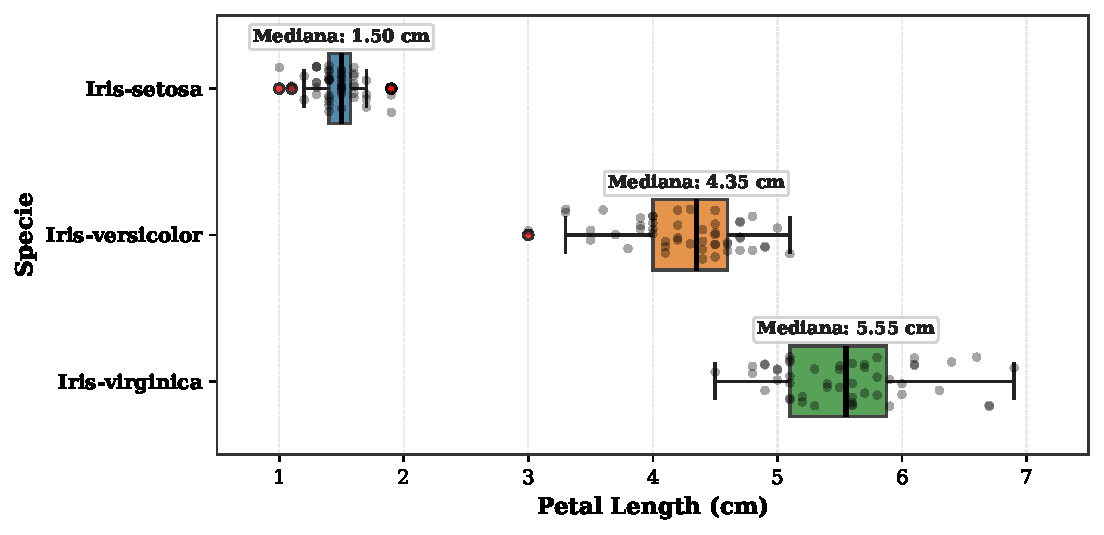
\includegraphics[width=0.88\textwidth]{iris_conditional_boxplot.pdf}
\caption{Box Plot condizionale calcolato sui dati reali del dataset Iris: distribuzione empirica della lunghezza del petalo (\textit{Petal Length}) stratificata sulle tre specie, con evidenza della mediana, dei quartili e dei singoli campioni osservati.}
\label{fig:iris-conditional-boxplot}
\end{figure}

\paragraph{Limiti del Box Plot rispetto agli Istogrammi:}
Sebbene il box plot sintetizzi efficacemente posizione e dispersione, **non permette di identificare la multimodalit\`a**. Due distribuzioni, una marcatamente bimodale e una unimodale simmetrica, possono presentare lo stesso Five-Number Summary ($x_{\min}, Q_1, Q_2, Q_3, x_{\max}$) generando lo stesso identico box plot; solo l'istogramma consente di visualizzare la presenza di una concavit\`a o di picchi multipli tra i quartili.

\chapter{Data Understanding II -- Analisi Multivariata, Correlazione e Rilevamento Outliers}
\label{chap:dm-data-understanding-multivariate-outliers}

L'analisi multivariata studia le relazioni simultanee tra due o più attributi del dataset, superando i limiti delle descrizioni univariata isolate. In questo capitolo si approfondiscono le tecniche di visualizzazione per dati a più dimensioni, gli indici formali di associazione e correlazione lineare e non lineare, i criteri metodologici per la diagnosi degli outlier e una checklist operativa conclusiva per completare la fase di Data Understanding.

Il caso di studio impiegato come riferimento applicativo è il benchmark \textbf{Iris} (introdotto dal botanico Edgar Anderson e reso celebre da Ronald Fisher nel 1936), composto da $150$ osservazioni distribuite in modo bilanciato su $3$ classi da $50$ campioni ciascuna (\textit{Iris setosa}, \textit{Iris versicolor}, \textit{Iris virginica}) e descritto da $4$ feature continue espresse in centimetri:
\begin{itemize}[noitemsep]
    \item Lunghezza del sepalo (\textit{Sepal Length})
    \item Larghezza del sepalo (\textit{Sepal Width})
    \item Lunghezza del petalo (\textit{Petal Length})
    \item Larghezza del petalo (\textit{Petal Width})
\end{itemize}

% ====================================================================
% SEZIONE 3.1: TECNICHE DI VISUALIZZAZIONE MULTIDIMENSIONALE
% ====================================================================
\section{Tecniche di Visualizzazione Multidimensionale}
\label{sec:dm-multivariate-visualization}

Quando l'analisi si estende a configurazioni bivariate e multivariate, la rappresentazione grafica deve consentire la percezione immediata della separabilità geometrica tra classi, dell'addensamento in cluster naturali e della presenza di anomalie strutturali.

\subsection{Scatter Plot e Scatter Matrix}

Lo \textbf{Scatter Plot (Grafico a Dispersione)} traccia ogni coppia di attributi continui $(X, Y)$ proiettando le osservazioni come punti con coordinate cartesiane $(x_i, y_i) \in \mathbb{R}^2$.
\begin{itemize}
    \item \textbf{Caratteristiche}: Permette di evidenziare visivamente cluster, tendenze di correlazione diretta o inversa e la presenza di outlier bivariati che risultano invisibili dall'analisi dei singoli istogrammi.
    \item \textbf{Codifica cromatico-categoriale}: Assegnando a ciascun punto un colore o un simbolo corrispondente alla classe di appartenenza, l'analista può valutare la separabilità geometrica indotta dalla coppia di feature.
    \item \textbf{Evidenza sul dataset Iris}: Incrociando \textit{Petal Length} e \textit{Petal Width}, le classi mostrano un elevato grado di separabilità: la classe \textit{Setosa} forma un cluster compatto e isolato, mentre \textit{Versicolor} e \textit{Virginica} presentano solo una ridotta sovrapposizione marginale (Figura~\ref{fig:dm-iris-scatter}). Al contrario, il piano formato da \textit{Sepal Length} e \textit{Sepal Width} mostra una forte sovrapposizione tra \textit{Versicolor} e \textit{Virginica}.
\end{itemize}

\begin{figure}[htbp]
    \centering
    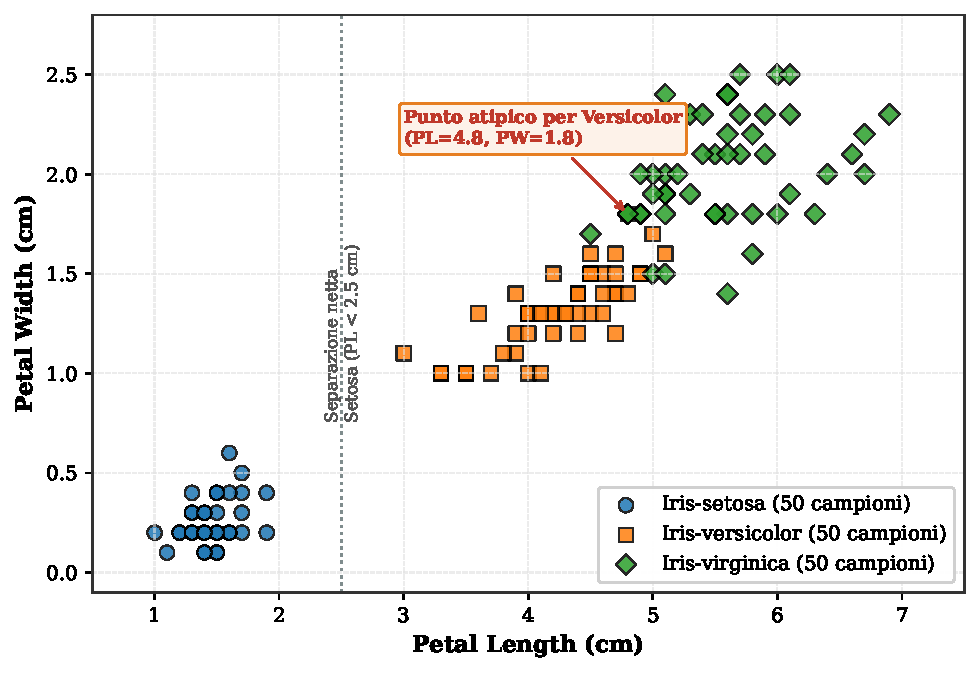
\includegraphics[width=0.88\textwidth]{iris_scatterplot_real.pdf}
    \caption{Scatter plot bivariati sul dataset Iris: confronto tra la separabilità generata da sepalo e petalo.}
    \label{fig:dm-iris-scatter}
\end{figure}

Quando il numero di attributi numerici $p$ è moderato ($3 \le p \le 10$), si ricorre alla \textbf{Scatter Matrix (Scatter Plot Matrix - SPLOM)}: una griglia simmetrica di dimensione $p \times p$ contenente tutti i $\frac{p(p-1)}{2}$ grafici a dispersione a coppie distinte.
Sulla diagonale principale vengono tipicamente inseriti gli istogrammi univariati o le stime di densità (KDE) della singola variabile, consentendo una diagnosi simultanea di forma e correlazione (Figura~\ref{fig:dm-iris-splom}).

\begin{figure}[htbp]
    \centering
    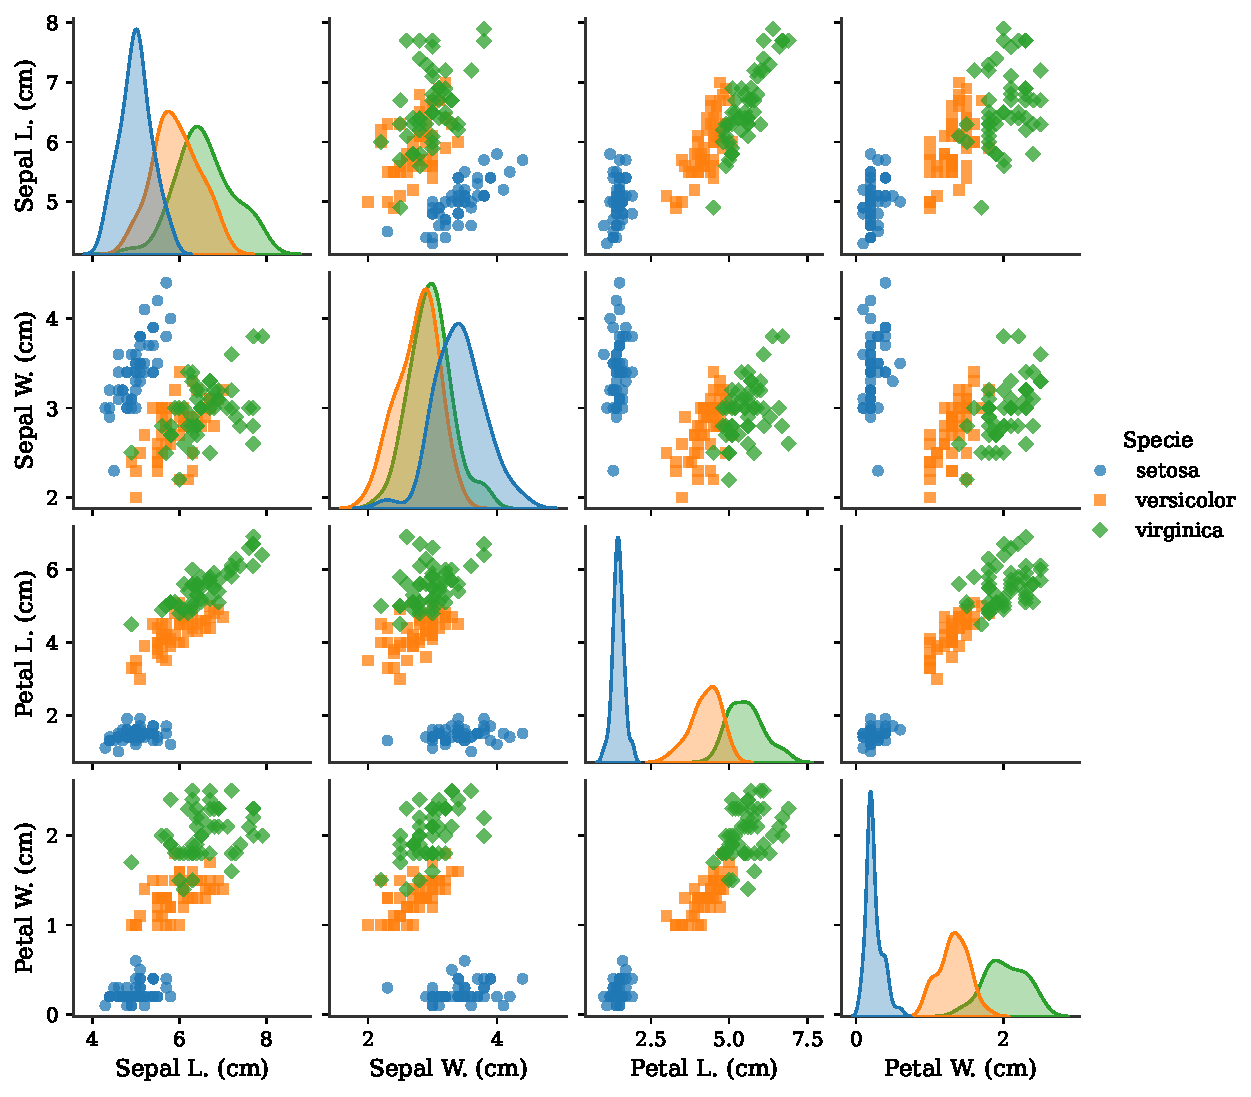
\includegraphics[width=0.88\textwidth]{iris_splom_real.pdf}
    \caption{Scatter Plot Matrix (SPLOM) completa per le quattro feature del dataset Iris.}
    \label{fig:dm-iris-splom}
\end{figure}

Lo \textbf{Scatter Plot Tridimensionale (3D)} estende la proiezione a tre coordinate cartesiane simultanee $(X_1, X_2, X_3)$. Consente di identificare outlier tridimensionali non rilevabili nelle proiezioni bidimensionali marginali, sebbene la fruizione su supporto bidimensionale risenta delle occlusioni e dell'angolazione di visuale.

\subsection{Visualizzazione di Spazi ad Alta Dimensionalità}

Negli spazi a dimensione elevata ($p > 3$), la geometria euclidea cartesiana classica non consente proiezioni dirette esaustive. Si adottano schemi grafici alternativi basati su geometrie coordinate non ortogonali.

\subsubsection{Coordinate Parallele (Parallel Coordinates)}
Nelle coordinate parallele gli assi non sono mutuamente perpendicolari, ma disposti come $p$ rette verticali equi-spaziate e parallele, ciascuna tarata sull'intervallo di valori dell'attributo corrispondente.

\begin{itemize}
    \item \textbf{Mappatura geometrica}: Un'osservazione $p$-dimensionale $\mathbf{x}_i = (x_{i1}, x_{i2}, \dots, x_{ip}) \in \mathbb{R}^p$ viene rappresentata non come un punto, ma come una \textbf{polilinea (linea spezzata)} che attraversa tutti gli assi, intersecando l'asse $j$-esimo esattamente alla quota $x_{ij}$.
    \item \textbf{Proprietà diagnostiche}: I record appartenenti alla stessa classe formano fasci compatti con andamento coerente. Una polilinea isolata con traiettoria discordante segnala un potenziale outlier multivariato.
    \item \textbf{Rilevanza dell'ordinamento degli assi}: La percezione dei legami statistici dipende dall'ordinamento orizzontale degli assi. Collocando attributi fortemente correlati su assi contigui, fasci di segmenti paralleli indicano correlazione positiva, mentre fasci che si incrociano a X indicano correlazione negativa (Figura~\ref{fig:dm-iris-parallel}).
\end{itemize}

\begin{figure}[htbp]
    \centering
    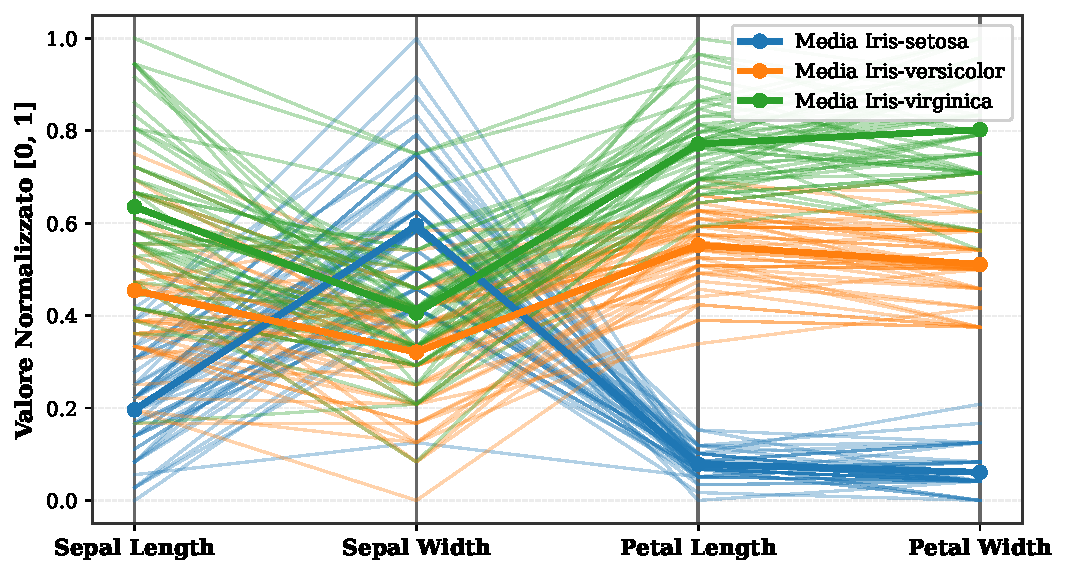
\includegraphics[width=0.88\textwidth]{iris_parallel_coordinates.pdf}
    \caption{Coordinate parallele per il dataset Iris con curve differenziate per classe.}
    \label{fig:dm-iris-parallel}
\end{figure}

\subsubsection{Radar Plot (Grafico Radar o Diagramma a Stella)}
Il \textbf{Radar Plot} condivide il principio delle coordinate parallele, con la variante che gli assi dimensionali non sono disposti linearmente, ma \textbf{irradiano a raggiera da un polo centrale comune}, distanziati da angoli equi-spaziati:
\begin{equation}
    \theta_j = \frac{2\pi (j-1)}{p}, \quad j = 1, \dots, p
\end{equation}

Per ciascun record, il valore assunto dalla variabile definisce la distanza del vertice dal centro lungo il corrispondente raggio; congiungendo i vertici si genera un poligono chiuso.
Quando il radar plot viene replicato in piccoli riquadri separati per ciascuna osservazione, prende il nome di \textbf{Star Plot}, agevolando il confronto visivo di profili complessi (Figura~\ref{fig:dm-iris-radar}).

\begin{figure}[htbp]
    \centering
    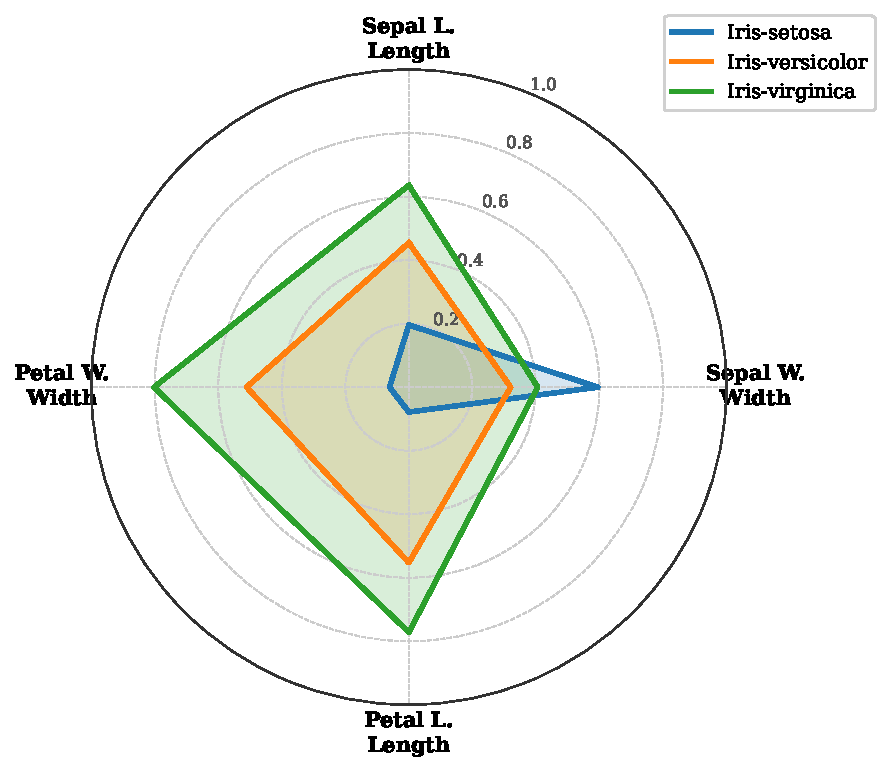
\includegraphics[width=0.82\textwidth]{iris_radar_plot.pdf}
    \caption{Profili medi delle classi del dataset Iris visualizzati tramite Radar Plot.}
    \label{fig:dm-iris-radar}
\end{figure}

% ====================================================================
% SEZIONE 3.2: COVARIANZA E CORRELAZIONE
% ====================================================================
\section{Analisi di Dipendenza Bivariata: Covarianza e Correlazione}
\label{sec:dm-covariance-correlation}

L'analisi quantitativa della dipendenza studia l'intensità e la direzione con cui due variabili casuali variano congiuntamente.

\subsection{Da Varianza a Covarianza}

Mentre la varianza misura la dispersione di una singola variabile rispetto al proprio baricentro, la \textbf{Covarianza Campionaria} quantifica la tendenza di due variabili numeriche $X$ e $Y$ a manifestare scarti concordi o discordi rispetto alle rispettive medie:
\begin{equation}
    \text{Cov}(X, Y) = s_{xy} = \frac{1}{n-1} \sum_{i=1}^n (x_i - \bar{x})(y_i - \bar{y})
\end{equation}

Nel caso speciale $X = Y$, la covarianza coincide con la varianza campionaria:
\begin{equation}
    \text{Cov}(X, X) = \frac{1}{n-1} \sum_{i=1}^n (x_i - \bar{x})^2 = s_x^2
\end{equation}

\subsubsection{Matrice di Covarianza}
Per un insieme di $p$ attributi continui, la struttura complessiva di variabilità congiunta è sintetizzata dalla \textbf{Matrice di Covarianza} $V \in \mathbb{R}^{p \times p}$:
\begin{equation}
    V = \begin{bmatrix}
        \text{Cov}(X_1, X_1) & \text{Cov}(X_1, X_2) & \cdots & \text{Cov}(X_1, X_p) \\
        \text{Cov}(X_2, X_1) & \text{Cov}(X_2, X_2) & \cdots & \text{Cov}(X_2, X_p) \\
        \vdots & \vdots & \ddots & \vdots \\
        \text{Cov}(X_p, X_1) & \text{Cov}(X_p, X_2) & \cdots & \text{Cov}(X_p, X_p)
    \end{bmatrix}
\end{equation}
\begin{itemize}[noitemsep]
    \item Gli elementi diagonali $V_{jj} = \text{Var}(X_j) = s_j^2$ rappresentano le varianze marginali.
    \item Gli elementi extra-diagonali $V_{jk} = \text{Cov}(X_j, X_k)$ rappresentano le covarianze a coppie.
    \item Poiché $\text{Cov}(X_j, X_k) = \text{Cov}(X_k, X_j)$, la matrice $V$ è \textbf{simmetrica} ($V = V^T$) e semi-definita positiva ($V \succeq 0$).
\end{itemize}

\subsubsection{Interpretazione Geometrica dei Prodotti degli Scarti}
Il segno della covarianza dipende dalla posizione delle osservazioni rispetto al baricentro $(\bar{x}, \bar{y})$ nel piano cartesiano, che divide lo spazio in quattro quadranti:

\begin{figure}[htbp]
    \centering
    \begin{tikzpicture}[scale=0.95]
        \draw[thick, -Stealth, color=gray!80!black] (-3.8, 0) -- (4.2, 0) node[right, font=\small] {$X$};
        \draw[thick, -Stealth, color=gray!80!black] (0, -3.2) -- (0, 3.5) node[above, font=\small] {$Y$};
        
        \draw[dashed, thick, color=navy!70] (0.5, -3.0) -- (0.5, 3.2);
        \draw[dashed, thick, color=navy!70] (-3.5, 0.4) -- (3.8, 0.4);
        
        \node[below right, font=\footnotesize\bfseries, color=navy] at (0.5, 0) {$\bar{x}$};
        \node[above left, font=\footnotesize\bfseries, color=navy] at (0, 0.4) {$\bar{y}$};
        
        % Quadrante I
        \node[draw=navy!30, fill=navy!4, rounded corners=3pt, align=center, font=\scriptsize, inner sep=4pt] at (2.5, 2.6) {
            \textbf{Quadrante I}\\
            $(x_i > \bar{x}) \land (y_i > \bar{y})$\\
            Scarto: $(+) \cdot (+) = \mathbf{(+)}$
        };
        \fill[crimson] (1.2, 0.9) circle (2.2pt);
        \fill[crimson] (1.7, 1.3) circle (2.2pt);
        \fill[crimson] (2.2, 1.7) circle (2.2pt);
        
        % Quadrante II
        \node[draw=navy!30, fill=navy!4, rounded corners=3pt, align=center, font=\scriptsize, inner sep=4pt] at (-2.0, 2.6) {
            \textbf{Quadrante II}\\
            $(x_i < \bar{x}) \land (y_i > \bar{y})$\\
            Scarto: $(-) \cdot (+) = \mathbf{(-)}$
        };
        \fill[darkgreen] (-1.2, 1.2) circle (2.2pt);
        
        % Quadrante III
        \node[draw=navy!30, fill=navy!4, rounded corners=3pt, align=center, font=\scriptsize, inner sep=4pt] at (-2.0, -2.4) {
            \textbf{Quadrante III}\\
            $(x_i < \bar{x}) \land (y_i < \bar{y})$\\
            Scarto: $(-) \cdot (-) = \mathbf{(+)}$
        };
        \fill[crimson] (-0.8, -0.4) circle (2.2pt);
        \fill[crimson] (-1.4, -0.9) circle (2.2pt);
        \fill[crimson] (-2.1, -1.3) circle (2.2pt);
        
        % Quadrante IV
        \node[draw=navy!30, fill=navy!4, rounded corners=3pt, align=center, font=\scriptsize, inner sep=4pt] at (2.5, -2.4) {
            \textbf{Quadrante IV}\\
            $(x_i > \bar{x}) \land (y_i < \bar{y})$\\
            Scarto: $(+) \cdot (-) = \mathbf{(-)}$
        };
        \fill[darkgreen] (1.6, -0.9) circle (2.2pt);
    \end{tikzpicture}
    \caption{Scomposizione geometrica degli scarti in quattro quadranti centrati sul baricentro $(\bar{x}, \bar{y})$.}
    \label{fig:dm-covariance-quadrants}
\end{figure}

\begin{itemize}
    \item Punti nei quadranti I e III apportano contributi positivi: le deviazioni sono concordi $\implies \text{Cov}(X, Y) > 0$.
    \item Punti nei quadranti II e IV apportano contributi negativi: le deviazioni sono discordi $\implies \text{Cov}(X, Y) < 0$.
    \item Se le osservazioni si disperdono uniformemente nei quattro quadranti, i termini positivi e negativi si bilanciano, portando a $\text{Cov}(X, Y) \approx 0$.
\end{itemize}

\subsubsection{Limite Strutturale: Dipendenza dall'Unità di Misura}
La covarianza non è invariante per trasformazioni di scala. Se la variabile $X$ esprime un reddito in euro e viene convertita in migliaia di euro ($X' = X / 1000$), la covarianza si riduce di un fattore $1000$, nonostante la correlazione statistica rimanga immutata. Essa non consente quindi di confrontare coppie di attributi aventi ordini di grandezza o unità differenti.

\subsection{Coefficiente di Correlazione Lineare di Pearson}

Il \textbf{Coefficiente di Correlazione Lineare di Pearson ($r_{xy}$)} normalizza la covarianza dividendola per il prodotto delle deviazioni standard campionarie:
\begin{equation}
    r_{xy} = \frac{\text{Cov}(X, Y)}{s_x s_y} = \frac{\sum_{i=1}^n (x_i - \bar{x})(y_i - \bar{y})}{\sqrt{\sum_{i=1}^n (x_i - \bar{x})^2} \sqrt{\sum_{i=1}^n (y_i - \bar{y})^2}}
\end{equation}

\subsubsection{Proprietà Matematiche del Coefficiente $r_{xy}$}
\begin{enumerate}
    \item \textbf{Limitazione dell'intervallo}: Per la disuguaglianza di Cauchy-Schwarz nello spazio dei vettori centrati, il coefficiente è rigorosamente limitato nell'intervallo:
    \begin{equation}
        -1 \le r_{xy} \le +1
    \end{equation}
    \item \textbf{Invarianza di scala}: È un indice adimensionale, invariante rispetto a qualunque trasformazione lineare affine positiva ($X' = aX + b, Y' = cY + d$ con $a, c > 0$).
    \item \textbf{Correlazione lineare perfetta}:
    \begin{itemize}
        \item $r_{xy} = +1$: indica una perfetta relazione lineare positiva crescente; tutti i punti giacciono su una retta a pendenza positiva ($y = ax + b$, con $a > 0$).
        \item $r_{xy} = -1$: indica una perfetta relazione lineare negativa decrescente ($a < 0$).
    \end{itemize}
    \item \textbf{Assenza di relazione lineare}: Un valore $r_{xy} \approx 0$ denota \textbf{assenza di associazione lineare}, ma non implica l'indipendenza stocastica. Relazioni funzionali non lineari deterministiche (es. $Y = X^2$ con $X$ distribuita simmetricamente attorno all'origine) generano $r_{xy} = 0$, pur in presenza di una totale dipendenza.
\end{enumerate}

\begin{figure}[htbp]
    \centering
    \begin{tikzpicture}[scale=0.88]
        % Panel 1: r = +1.0
        \begin{scope}[shift={(0,0)}]
            \draw[->] (0,0) -- (2.5,0) node[below] {$X$};
            \draw[->] (0,0) -- (0,2.3) node[left] {$Y$};
            \draw[thick, color=crimson] (0.3,0.3) -- (2.2,2.0);
            \fill (0.5,0.48) circle (1.5pt);
            \fill (1.0,0.92) circle (1.5pt);
            \fill (1.5,1.38) circle (1.5pt);
            \fill (2.0,1.82) circle (1.5pt);
            \node[below, font=\scriptsize] at (1.25,-0.2) {$r = +1.0$};
            \node[below, font=\tiny, align=center] at (1.25,-0.6) {Lineare Positiva\\Perfetta};
        \end{scope}

        % Panel 2: r = -0.8
        \begin{scope}[shift={(3.8,0)}]
            \draw[->] (0,0) -- (2.5,0) node[below] {$X$};
            \draw[->] (0,0) -- (0,2.3) node[left] {$Y$};
            \draw[thick, dashed, color=navy] (0.3,2.0) -- (2.2,0.4);
            \fill (0.4,1.8) circle (1.5pt);
            \fill (0.7,1.7) circle (1.5pt);
            \fill (1.0,1.2) circle (1.5pt);
            \fill (1.3,1.4) circle (1.5pt);
            \fill (1.6,0.9) circle (1.5pt);
            \fill (1.9,0.5) circle (1.5pt);
            \node[below, font=\scriptsize] at (1.25,-0.2) {$r = -0.80$};
            \node[below, font=\tiny, align=center] at (1.25,-0.6) {Forte Associazione\\Lineare Negativa};
        \end{scope}

        % Panel 3: r = 0.0
        \begin{scope}[shift={(7.6,0)}]
            \draw[->] (0,0) -- (2.5,0) node[below] {$X$};
            \draw[->] (0,0) -- (0,2.3) node[left] {$Y$};
            \fill (0.5,0.5) circle (1.5pt); \fill (0.7,1.8) circle (1.5pt);
            \fill (1.2,1.1) circle (1.5pt); \fill (1.4,0.4) circle (1.5pt);
            \fill (1.8,1.7) circle (1.5pt); \fill (2.0,0.8) circle (1.5pt);
            \node[below, font=\scriptsize] at (1.25,-0.2) {$r \approx 0.0$};
            \node[below, font=\tiny, align=center] at (1.25,-0.6) {Nessun Legame\\Lineare};
        \end{scope}

        % Panel 4: r = 0.0 Non-lineare
        \begin{scope}[shift={(11.4,0)}]
            \draw[->] (0,0) -- (2.5,0) node[below] {$X$};
            \draw[->] (0,0) -- (0,2.3) node[left] {$Y$};
            \draw[thick, color=darkgreen, domain=0.3:2.2, samples=30] plot (\x, {2.0 - 1.8*(\x-1.25)*(\x-1.25)});
            \fill (0.4,0.7) circle (1.5pt); \fill (0.8,1.6) circle (1.5pt);
            \fill (1.25,2.0) circle (1.5pt); \fill (1.7,1.6) circle (1.5pt);
            \fill (2.1,0.7) circle (1.5pt);
            \node[below, font=\scriptsize] at (1.25,-0.2) {$r = 0.0$};
            \node[below, font=\tiny, align=center] at (1.25,-0.6) {Dipendenza\\Quadratica Curva};
        \end{scope}
    \end{tikzpicture}
    \caption{Configurazioni tipiche di dispersione bivariata e corrispondenti coefficienti $r$ di Pearson.}
    \label{fig:dm-pearson-scenarios}
\end{figure}

\begin{figure}[htbp]
    \centering
    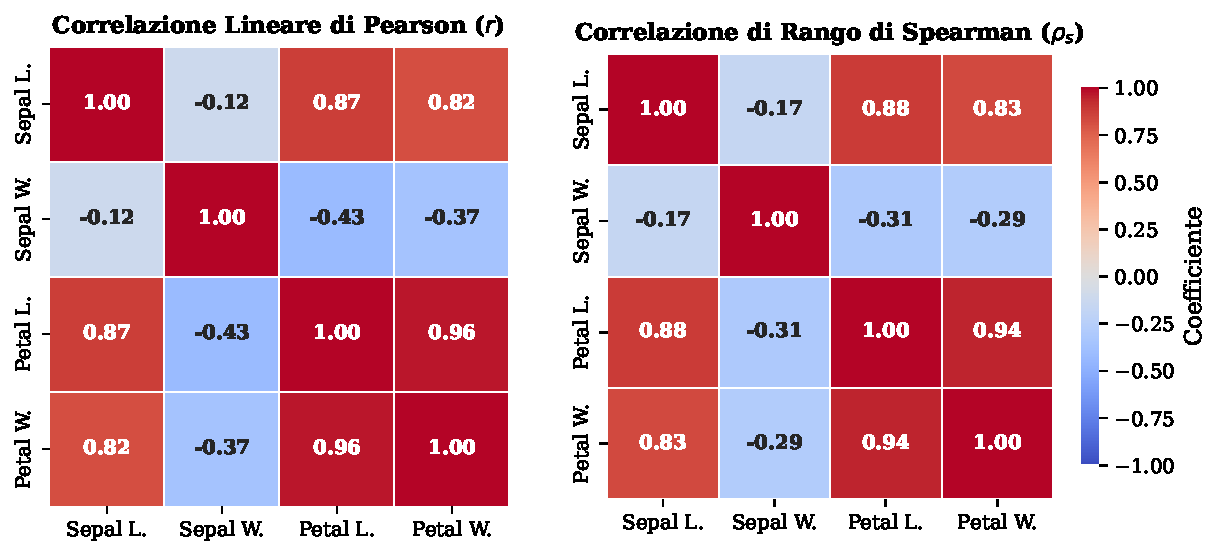
\includegraphics[width=0.88\textwidth]{iris_correlation_heatmaps.pdf}
    \caption{Heatmap di correlazione per il dataset Iris complessivo e disaggregato per singola specie.}
    \label{fig:dm-iris-heatmaps}
\end{figure}

\subsection{Fallacia Causale e Variabili Concomitanti}

Un principio fondante dell'analisi dati stabilisce che \textbf{la correlazione statistica non implica causalità} (\textit{correlation does not imply causation}). Un valore elevato di $|r_{xy}|$ può originare da tre dinamiche:
\begin{enumerate}
    \item $X$ è causa diretta di $Y$.
    \item $Y$ è causa diretta di $X$.
    \item $X$ e $Y$ sono entrambe causate da una terza variabile non osservata o latente, definita \textbf{variabile di confondimento (confounding factor)}.
\end{enumerate}

\begin{noteblock}{Esempio Classico: Vendita di Gelati e Annegamenti}
Durante i mesi estivi si registra una forte correlazione lineare positiva ($r > 0.85$) tra le vendite di gelati ($X$) e il numero di decessi per annegamento ($Y$). Dedurre che l'assunzione di gelati aumenti il rischio di annegamento costituisce una fallacia causale: entrambe le grandezze sono influenzate da un fattore di confondimento esogeno, la temperatura ambientale (\textit{hot weather}), che incentiva simultaneamente il consumo di gelati e l'afflusso di bagnanti in mare e nei fiumi.
\end{noteblock}

\subsection{Coefficiente di Correlazione per Ranghi di Spearman}

Quando i dati violano l'ipotesi di normalità bivariata o presentano relazioni non lineari ma strettamente monotone, si impiega il \textbf{Coefficiente di Correlazione per Ranghi di Spearman ($\rho$)}.

La procedura converte ciascun valore continuo $x_i$ e $y_i$ nella rispettiva posizione d'ordine o rango ordinale $r(x_i), r(y_i) \in \{1, \dots, n\}$. In assenza di valori paritari (\textit{ties}), la formulazione algebrica esplicita risulta:
\begin{equation}
    \rho = 1 - \frac{6 \sum_{i=1}^n \big(r(x_i) - r(y_i)\big)^2}{n(n^2 - 1)}
\end{equation}

\begin{itemize}[noitemsep]
    \item $\rho = +1$: indica una perfetta relazione monotona crescente (al crescere di $X$, $Y$ cresce strettamente, anche secondo andamenti esponenziali o sigmoidei).
    \item $\rho = -1$: indica una perfetta relazione monotona decrescente.
    \item \textbf{Robustezza}: Essendo basato sui ranghi ordinali anziché sui valori metrici effettivi, Spearman è molto meno sensibile a valori anomali isolati situati nelle code.
\end{itemize}

% ====================================================================
% SEZIONE 3.3: OUTLIER DETECTION
% ====================================================================
\section{Tassonomia e Rilevamento degli Outlier}
\label{sec:dm-outlier-detection-taxonomy}

Un \textbf{outlier} (valore anomalo) è definito come un'istanza che devia marcatamente dalla distribuzione della maggior parte delle osservazioni, suggerendo che sia stata generata da un meccanismo generatore differente o affetta da distorsioni di misura.

\subsection{Ruolo degli Outlier: Rumore vs Target di Analisi}
\begin{itemize}
    \item \textbf{Outlier come Rumore (Noise)}: L'anomalia è conseguenza di un errore materiale di digitazione, di un malfunzionamento momentaneo della sensoristica o di un'alterazione spuria. In questa veste, l'outlier degrada gli stimatori e deve essere isolato, corretto o rimosso in fase di pre-processing.
    \item \textbf{Outlier come Obiettivo Primario (Analysis Goal)}: L'indagine analitica è finalizzata precisamente all'identificazione di eventi eccezionali, che veicolano il massimo valore informativo.
    \begin{itemize}[noitemsep]
        \item Rilevamento di intrusioni informatiche (\textit{Intrusion Detection}).
        \item Identificazione di frodi finanziarie o transazioni bancarie illecite.
        \item Manutenzione predittiva su macchinari industriali tramite rilievo di micro-vibrazioni anomale.
    \end{itemize}
\end{itemize}

\subsection{Metodologie di Identificazione degli Outlier}

La tassonomia degli approcci di identificazione distingue tra indagini su singola feature e indagini congiunte multidimensionali:

\begin{figure}[htbp]
    \centering
    \begin{tikzpicture}[
        outlierCard/.style={draw=navy!80!black, fill=navy!6, rounded corners=6pt, thick, font=\footnotesize, align=left, text width=6.0cm, minimum height=2.8cm, inner sep=6pt},
        arrowStyle/.style={-Stealth, thick, draw=navy!85!black}
    ]
        % Root
        \node[rectangle, rounded corners=6pt, draw=purple!85!black, fill=purple!12, very thick, font=\small\bfseries, align=center, text width=10.2cm, inner sep=6pt] (root) at (0, 2.7) {
            TASSONOMIA DEL RILEVAMENTO OUTLIER\\[2pt]
            \footnotesize \normalfont Criteri per feature singole e spazi multidimensionali
        };

        % Ramo Sinistro: Univariati
        \node[outlierCard, anchor=north] (uniCol) at (-3.6, 1.1) {
            \textbf{Metodi Univariati}\\[4pt]
            $\bullet$ \textbf{IQR (Tukey)}: Boxplot $[L, U]$\\[3pt]
            $\bullet$ \textbf{Z-Score}: Soglia $|z| > 3.29$\\[3pt]
            $\bullet$ \textbf{Frequenza}: Valori rari ($< 0.1\%$)
        };

        % Ramo Destro: Multidimensionali
        \node[outlierCard, anchor=north] (multiCol) at (3.6, 1.1) {
            \textbf{Metodi Multidimensionali}\\[4pt]
            $\bullet$ \textbf{Scatter / SPLOM}: Punti dispersi\\[3pt]
            $\bullet$ \textbf{PCA}: Varianza residua anomala\\[3pt]
            $\bullet$ \textbf{Clustering / LOF}: Bassa densit\`a
        };

        \coordinate (split) at (0, 1.65);
        \draw[thick, draw=navy!85!black] (root.south) -- (split);
        \draw[arrowStyle] (split) -| (uniCol.north);
        \draw[arrowStyle] (split) -| (multiCol.north);
    \end{tikzpicture}
    \caption{Tassonomia delle metodologie di rilevamento delle anomalie.}
    \label{fig:dm-outlier-taxonomy}
\end{figure}

\begin{itemize}
    \item \textbf{Attributi Categorici}: Un'osservazione anomala presenta una categoria associata a una frequenza empirica prossima allo zero ($< 0.1\%$).
    \item \textbf{Attributi Numerici Univariati}:
    \begin{itemize}[noitemsep]
        \item \textit{Regola di Tukey}: Valori esterni all'intervallo $[Q_1 - 1.5\,\text{IQR},\, Q_3 + 1.5\,\text{IQR}]$.
        \item \textit{Criterio Z-Score}: Valori con scostamento standardizzato $|z| > 3.29$ (code estreme della normale).
    \end{itemize}
    \item \textbf{Spazi Multidimensionali}:
    \begin{itemize}[noitemsep]
        \item \textit{Scatter Plot bivariati}: Identificazione ottica di punti lontani dal corpo centrale della nube.
        \item \textit{Proiezioni PCA}: Punti che presentano valori anomali lungo le componenti principali secondarie.
        \item \textit{Clustering e Local Outlier Factor (LOF)}: Riconoscimento di punti isolati a bassa densità locale rispetto al vicinato di $k$ elementi.
    \end{itemize}
\end{itemize}

% ====================================================================
% SEZIONE 3.4: GESTIONE DEI VALORI MANCANTI
% ====================================================================
\section{Gestione dei Valori Mancanti}
\label{sec:dm-missing-values-intro}

Un record manifesta \textbf{valori mancanti (Missing Values)} quando per una o più feature non è presente alcuna informazione registrata (formalmente denotata con simboli nulli come \texttt{NaN}, \texttt{NULL}, \texttt{?} o mediante valori convenzionali impliciti come \texttt{999} o \texttt{0}).

\subsection{Cause di Insorgenza}
\begin{enumerate}
    \item \textbf{Omissione volontaria per riservatezza}: L'intervistato si rifiuta di comunicare attributi sensibili (es. reddito personale, orientamento politico o religioso, abitudini sanitarie).
    \item \textbf{Inapplicabilità logica del campo}: La variabile non è definita per una specifica sottopopolazione (es. il numero di gravidanze per individui di sesso maschile, o l'anzianità lavorativa per minori in età scolare).
    \item \textbf{Avarie strumentali o caduta di connettività}: Malfunzionamento di sensori di telemetria che generano valori nulli o trasmettono serie fittizie costanti (es. sensore anemometrico bloccato che registra sistematicamente velocità del vento pari a $0\,\text{m/s}$).
\end{enumerate}

\subsection{Checklist Operativa per il Data Understanding}

A completamento della fase di esplorazione preliminare, l'analista deve verificare sistematicamente la seguente checklist:

\begin{table}[htbp]
    \centering
    \small
    \begin{tabularx}{\textwidth}{lX}
        \toprule
        \textbf{Ambito di Controllo} & \textbf{Verifica Diagnostica da Eseguire} \\
        \midrule
        \textbf{Coerenza Sintattica} & Verificare i tipi di dato, la codifica di formati numerici/stringa e i vincoli di dominio. \\
        \textbf{Valori Anomali (Outlier)} & Ispezionare la presenza di valori estremi mediante Boxplot univariati e Scatter Plot bivariati. \\
        \textbf{Valori Mancanti (Missing)} & Rilevare incidenza percentuale dei campi nulli e identificare valori sentinella impliciti (\texttt{0}, \texttt{-1}, \texttt{999}). \\
        \textbf{Associazioni e Ridondanze} & Calcolare le correlazioni di Pearson e Spearman per isolare coppie di attributi collineari o ridondanti. \\
        \textbf{Assunzioni Distributive} & Verificare simmetria, normalità e omoschedasticità prima di impostare la fase di preparazione e pulizia. \\
        \bottomrule
    \end{tabularx}
    \caption{Checklist diagnostica operativa per la chiusura della fase di Data Understanding.}
    \label{tab:dm-du-checklist}
\end{table}

\chapter{Data Preparation \& Cleaning -- Riduzione, Discretizzazione e Trasformazione}
\label{chap:dm-data-preparation-cleaning}

Mentre la fase di Data Understanding si concentra sulla diagnosi delle anomalie e sulla comprensione delle strutture latenti del dataset, la \textbf{Data Preparation} costituisce la componente operativa e trasformativa del ciclo KDD. In questa fase i dati grezzi vengono bonificati, compressi, riscalati e ricodificati per soddisfare i requisiti algebrici e computazionali degli algoritmi di data mining.

% ====================================================================
% SEZIONE 4.1: DIFFERENZE TRA DATA UNDERSTANDING E DATA PREPARATION
% ====================================================================
\section{Differenze tra Data Understanding e Data Preparation}
\label{sec:dm-du-vs-dp}

La transizione tra la fase diagnostica e la fase trasformativa è sintetizzata dal passaggio dalle evidenze empiriche alle azioni di pulizia:

\begin{figure}[htbp]
    \centering
    \begin{tikzpicture}[
        box/.style={draw=navy, rounded corners, fill=navy!8, font=\small, text width=5.2cm, inner sep=6pt},
        arrow/.style={-Stealth, thick, color=navy}
    ]
        \node[box] (du) {
            \centering \textbf{DATA UNDERSTANDING}\\
            \textit{(Fase Diagnostica)}\\[4pt]
            \raggedright
            $\bullet$ Rileva valori mancanti\\
            $\bullet$ Identifica outlier univariati/multivariati\\
            $\bullet$ Misura correlazioni elevate e collinearità\\
            $\bullet$ Diagnostica asimmetrie distributive\\
            $\bullet$ Rileva scale eterogenee
        };
        
        \node[box, right=2.0cm of du] (dp) {
            \centering \textbf{DATA PREPARATION}\\
            \textit{(Fase Interventistica)}\\[4pt]
            \raggedright
            $\bullet$ Imputa o rimuove i missing\\
            $\bullet$ Gestisce/Winsorizza gli outlier\\
            $\bullet$ Rimuove feature ridondanti\\
            $\bullet$ Applica trasformazioni logaritmiche/Box-Cox\\
            $\bullet$ Normalizza (Min-Max, Z-Score)
        };
        
        \draw[arrow] (du.east) -- (dp.west) node[midway, above, font=\footnotesize, color=navy] {Informa};
    \end{tikzpicture}
    \caption{Relazione sequenziale tra Data Understanding (diagnosi) e Data Preparation (intervento).}
    \label{fig:dm-du-vs-dp}
\end{figure}

% ====================================================================
% SEZIONE 4.2: AGGREGAZIONE E CAMPIONAMENTO
% ====================================================================
\section{Aggregazione e Campionamento}
\label{sec:dm-aggregation-sampling}

La riduzione del volume dei dati si persegue mediante la combinazione di osservazioni o attraverso la selezione statistica di sottoinsiemi rappresentativi.

\subsection{Aggregazione dei Dati}

L'aggregazione sintetizza due o più record o attributi in una singola misura aggregata.
\begin{itemize}
    \item \textbf{Obiettivi primari}:
    \begin{enumerate}
        \item \textit{Riduzione dimensionale}: Riduce il numero complessivo di record o attributi, alleggerendo il carico computazionale.
        \item \textit{Riconfigurazione di scala e granularità}: Adatta l'analisi al livello concettuale idoneo (ad esempio, aggregare le transazioni orarie in totali settimanali o i singoli punti vendita a livello regionale).
        \item \textit{Stabilizzazione della varianza}: Le grandezze aggregate mediano il rumore casuale, producendo indicatori a varianza inferiore e relazioni più stabili.
    \end{enumerate}
    \item \textbf{Caso Studio: Precipitazioni in Australia (1982--1993)}: Nelle serie storiche pluviometriche australiane, la deviazione standard delle precipitazioni medie mensili evidenzia un'elevata variabilità con code fino a $15\,\text{cm}$. Al contrario, aggregando i dati su base annua, la deviazione standard si concentra su valori bassi con dispersione contenuta (Figura~\ref{fig:dm-precip-aggregation}). Per l'analisi dei cicli stagionali è necessaria la scala mensile disaggregata, mentre per la comparazione dei regimi climatici regionali la scala annua aggregata risulta più robusta e priva del rumore a breve termine.
\end{itemize}

\begin{figure}[htbp]
    \centering
    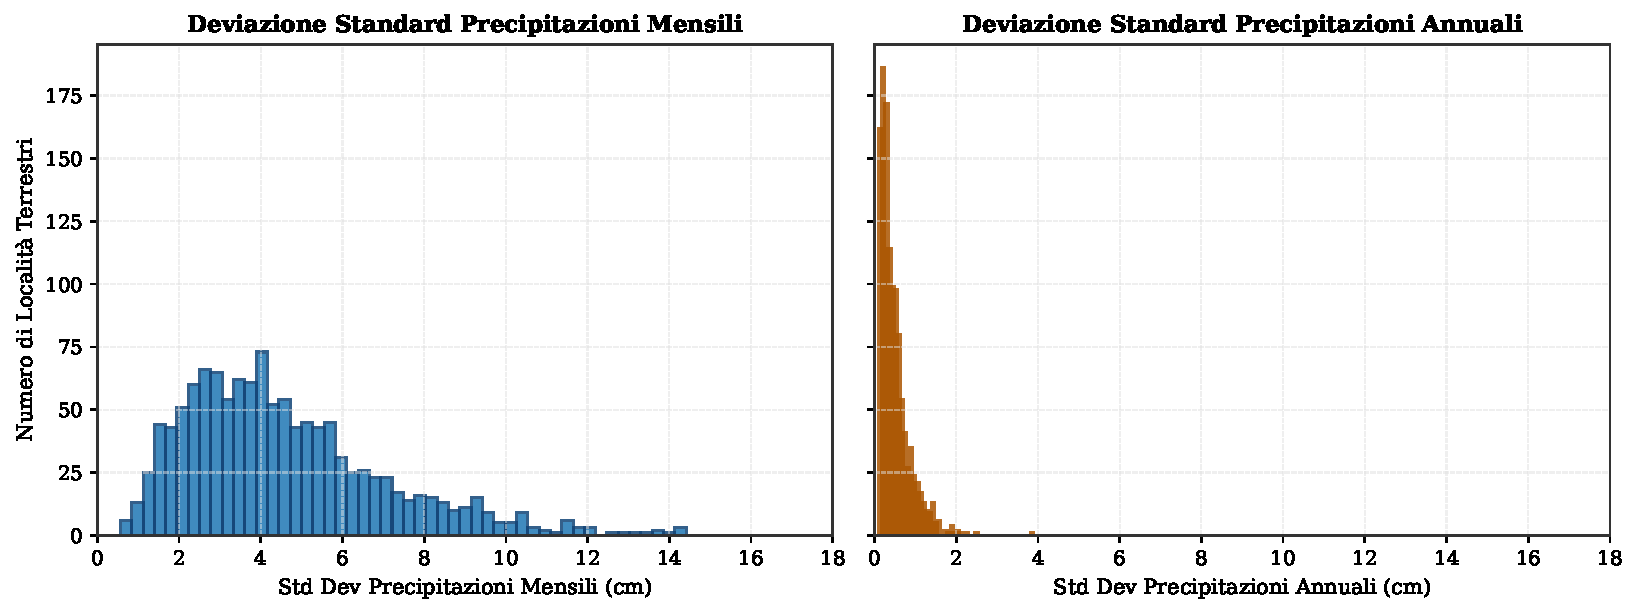
\includegraphics[width=0.88\textwidth]{precipitation_aggregation.pdf}
    \caption{Confronto di dispersione tra precipitazioni medie mensili e precipitazioni medie annue aggregate in Australia.}
    \label{fig:dm-precip-aggregation}
\end{figure}

\subsection{Tecniche di Campionamento (Sampling)}

Il campionamento estrae un sottoinsieme rappresentativo di dimensione $n$ da una popolazione complessiva di cardinalità $N$ ($n \ll N$).
Un campione è \textbf{rappresentativo} se riflette fedelmente le medesime proprietà distributive e statistiche della popolazione sorgente.

\begin{figure}[htbp]
    \centering
    \begin{tikzpicture}[
        sampleCard/.style={draw=navy!80!black, fill=navy!6, rounded corners=6pt, thick, font=\footnotesize, align=left, text width=6.0cm, minimum height=2.8cm, inner sep=6pt},
        arrowStyle/.style={-Stealth, thick, draw=navy!85!black}
    ]
        % Root
        \node[rectangle, rounded corners=6pt, draw=purple!85!black, fill=purple!12, very thick, font=\small\bfseries, align=center, text width=10.0cm, inner sep=6pt] (root) at (0, 2.7) {
            STRATEGIE DI CAMPIONAMENTO\\[2pt]
            \footnotesize \normalfont Tecniche per l'estrazione di sottoinsiemi rappresentativi
        };

        % Left branch: SRS
        \node[sampleCard, anchor=north] (srsCol) at (-3.6, 1.1) {
            \textbf{Casuale Semplice (SRS)}\\[4pt]
            $\bullet$ \textbf{Senza Replica}: Prelievi univoci\\[3pt]
            $\bullet$ \textbf{Con Replica}: Duplicati ammessi\\[3pt]
            $\bullet$ \textbf{Probabilit\`a}: Uniforme ($P = 1/N$)
        };

        % Right branch: Stratified
        \node[sampleCard, anchor=north] (stratCol) at (3.6, 1.1) {
            \textbf{Campionamento Stratificato}\\[4pt]
            $\bullet$ \textbf{Strati}: Gruppi omogenei disgiunti\\[3pt]
            $\bullet$ \textbf{Quote}: Estrazione proporzionale\\[3pt]
            $\bullet$ \textbf{Obiettivo}: Protezione classi rare
        };

        \coordinate (split) at (0, 1.65);
        \draw[thick, draw=navy!85!black] (root.south) -- (split);
        \draw[arrowStyle] (split) -| (srsCol.north);
        \draw[arrowStyle] (split) -| (stratCol.north);
    \end{tikzpicture}
    \caption{Albero delle strategie di campionamento nel data mining.}
    \label{fig:dm-sampling-tree}
\end{figure}

\begin{enumerate}
    \item \textbf{Campionamento Casuale Semplice (Simple Random Sampling)}: Ciascuna istanza possiede la medesima probabilità a priori di selezione:
    \begin{equation}
        P(x_i) = \frac{1}{N}
    \end{equation}
    \begin{itemize}[noitemsep]
        \item \textit{Senza reinserimento (without replacement)}: L'elemento estratto viene rimosso dal pool e non può essere riselezionato.
        \item \textit{Con reinserimento (with replacement)}: L'elemento estratto rimane disponibile per successive estrazioni (stesso record estratto $> 1$ volta).
    \end{itemize}
    \item \textbf{Campionamento Stratificato (Stratified Sampling)}: La popolazione viene suddivisa in strati omogenei disgiunti (ad esempio per etichetta di classe o per percentili). Da ciascun strato viene estratto un campione proporzionale alla sua cardinalità relativa, garantendo che le classi rare non vengano omesse dal campione estratto.
\end{enumerate}

La scelta della dimensione campionaria ottimale impone un compromesso tra costo computazionale e accuratezza statistica, come illustrato nella curva di trade-off di Figura~\ref{fig:dm-sampling-tradeoff}.

\begin{figure}[htbp]
    \centering
    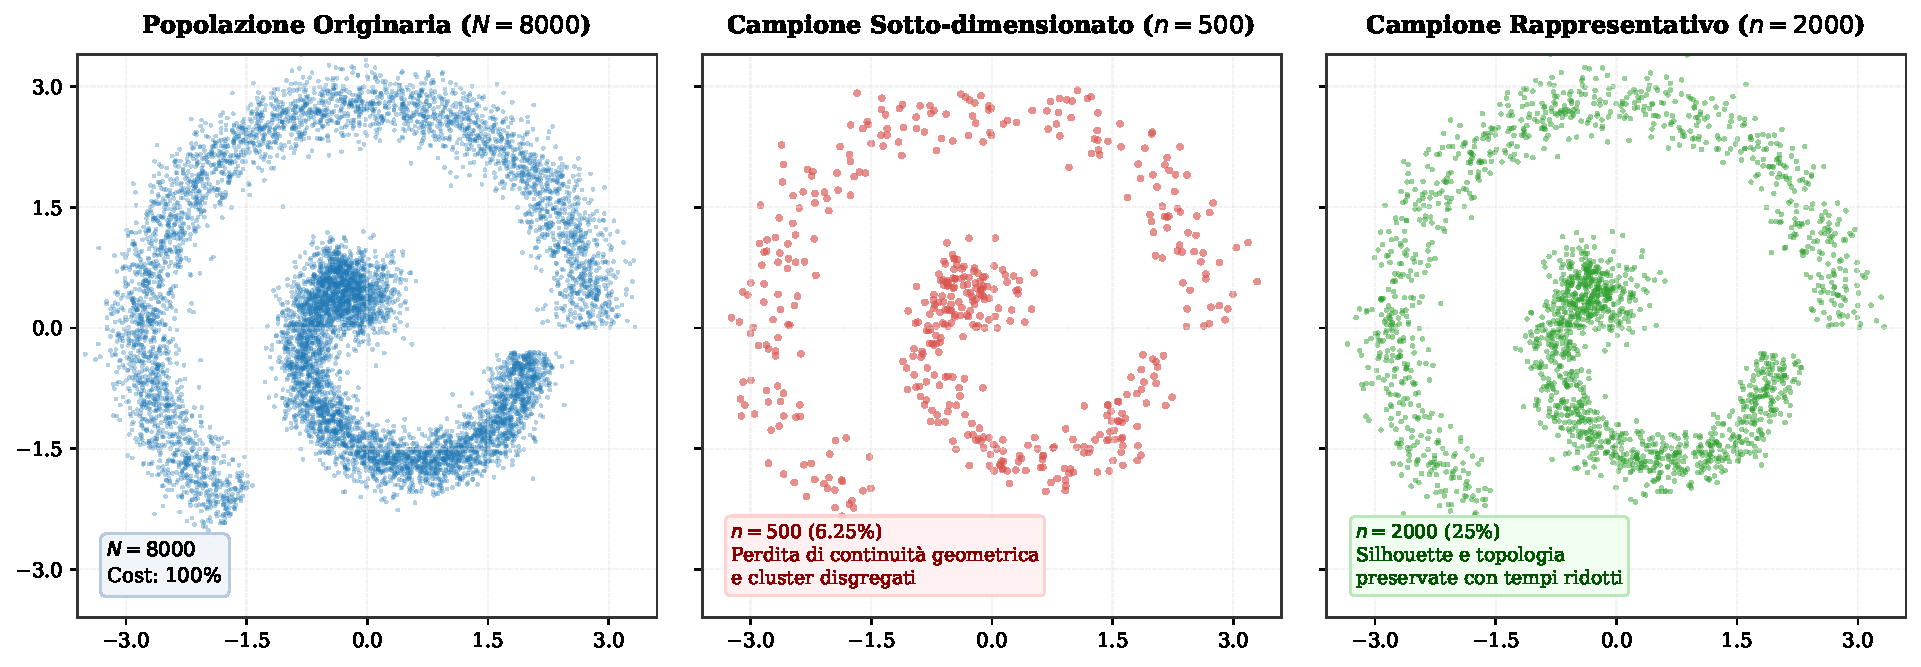
\includegraphics[width=0.82\textwidth]{sampling_tradeoff.pdf}
    \caption{Trade-off tra dimensione campionaria e accuratezza empirica di stima.}
    \label{fig:dm-sampling-tradeoff}
\end{figure}

% ====================================================================
% SEZIONE 4.3: RIDUZIONE DELLA DIMENSIONALITA'
% ====================================================================
\section{Riduzione della Dimensionalità}
\label{sec:dm-dimensionality-reduction}

La presenza di un numero elevato di feature determina rilevanti criticità computazionali e geometriche.

\subsection{La Maledizione della Dimensionalità (\textit{Curse of Dimensionality})}
\label{subsec:dm-curse-of-dimensionality}

All'aumentare della dimensionalità $p$, il volume dello spazio $\mathbb{R}^p$ cresce esponenzialmente rispetto al numero di osservazioni disponibili. Questo fenomeno causa:
\begin{enumerate}
    \item \textbf{Sparsità estrema}: Le osservazioni si disperdono nello spazio multidimensionale; la densità locale tende a zero e lo spazio diventa prevalentemente vuoto.
    \item \textbf{Concentrazione delle distanze}: All'aumentare di $p$, il contrasto relativo tra la distanza minima e la distanza massima rispetto a qualsiasi punto di riferimento tende a vanificarsi:
    \begin{equation}
        \lim_{p \to \infty} \frac{\mathrm{dist}_{\max} - \mathrm{dist}_{\min}}{\mathrm{dist}_{\min}} \to 0
    \end{equation}
    Ciò compromette le prestazioni degli algoritmi metrica-dipendenti ($k$-NN, clustering K-Means).
    \item \textbf{Instabilità delle stime}: La stima della matrice di covarianza $p \times p$ richiede una numerosità campionaria che scala esponenzialmente con $p$ per scongiurare singolarità numeriche.
\end{enumerate}

\begin{figure}[htbp]
    \centering
    \begin{tikzpicture}[scale=0.9]
        % 1D
        \begin{scope}[shift={(0,0)}]
            \draw[thick, <->] (0,0) -- (3,0);
            \foreach \x in {0.3, 0.7, 1.1, 1.5, 1.8, 2.2, 2.7} {
                \fill[crimson] (\x, 0) circle (2pt);
            }
            \node[below, font=\footnotesize] at (1.5,-0.3) {\textbf{1D}: Spazio Denso};
            \node[below, font=\tiny, align=center] at (1.5,-0.7) {7 punti in 1 unità};
        \end{scope}
        
        % 2D
        \begin{scope}[shift={(4.5, -0.8)}]
            \draw[step=0.6, gray!60, very thin] (0,0) grid (2.4, 2.4);
            \draw[thick] (0,0) rectangle (2.4, 2.4);
            \fill[crimson] (0.3, 1.5) circle (2pt);
            \fill[crimson] (1.5, 0.9) circle (2pt);
            \fill[crimson] (2.1, 2.1) circle (2pt);
            \node[below, font=\footnotesize] at (1.2,-0.2) {\textbf{2D}: Densità Ridotta};
            \node[below, font=\tiny, align=center] at (1.2,-0.6) {16 celle (alcune vuote)};
        \end{scope}
        
        % 3D
        \begin{scope}[shift={(9.0, -0.8)}]
            \draw[thick] (0,0) rectangle (2,2);
            \draw[thick] (0.8,0.8) rectangle (2.8,2.8);
            \draw[thick] (0,0) -- (0.8,0.8);
            \draw[thick] (2,0) -- (2.8,0.8);
            \draw[thick] (2,2) -- (2.8,2.8);
            \draw[thick] (0,2) -- (0.8,2.8);
            \fill[crimson] (1.2, 1.4) circle (2pt);
            \node[below, font=\footnotesize] at (1.4,-0.2) {\textbf{3D}: Sparsità Critica};
            \node[below, font=\tiny, align=center] at (1.4,-0.6) {Spazio prevalentemente vuoto};
        \end{scope}
    \end{tikzpicture}
    \caption{Illustrazione della dispersione geometrica dei campioni all'aumentare delle dimensioni (Curse of Dimensionality).}
    \label{fig:dm-curse-dimensionality}
\end{figure}

\subsection{Selezione delle Feature (Feature Selection)}

La \textbf{Feature Selection} seleziona un sottoinsieme ottimale di feature originali, eliminando gli attributi irrilevanti (non informativi) e ridondanti (duplicati di informazione già presente). I metodi si suddividono in tre categorie:

\begin{table}[htbp]
    \centering
    \small
    \begin{tabularx}{\textwidth}{lXX}
        \toprule
        \textbf{Paradigma} & \textbf{Meccanismo Operativo} & \textbf{Vantaggi / Limiti} \\
        \midrule
        \textbf{Filter} & Valutano la significatività statistica ($t$-test, ANOVA, correlazione di Pearson, $\chi^2$) a priori, indipendentemente dal modello. & Computazionalmente velocissimi; non considerano l'interazione tra feature. \\
        \addlinespace
        \textbf{Wrapper} & Utilizzano il modello predittivo come oracolo di valutazione iterativo (Forward Selection, Backward Elimination). & Ottimizzano l'accuratezza finale; computazionalmente gravosi ($2^p$ combinazioni teoriche). \\
        \addlinespace
        \textbf{Embedded} & La selezione è integrata nel processo di addestramento dell'algoritmo (es. alberi decisionali, regolarizzazione Lasso $L_1$). & Eccellente compromesso tra accuratezza e tempi computazionali. \\
        \bottomrule
    \end{tabularx}
    \caption{Confronto sinottico tra approcci Filter, Wrapper ed Embedded per la Feature Selection.}
    \label{tab:dm-feature-selection-methods}
\end{table}

\subsection{Creazione e Proiezione di Feature}
\begin{itemize}
    \item \textbf{Costruzione di Feature (\textit{Feature Construction})}: Generazione di nuove variabili combinando attributi esistenti tramite conoscenza del dominio (ad esempio, calcolo della densità come $\text{massa}/\text{volume}$ o dell'efficienza come $\text{ore effettive}/\text{ore previste}$).
    \item \textbf{Proiezione di Feature (\textit{Feature Projection})}: Mappatura lineare o non lineare dello spazio originario $\mathbb{R}^p$ in un sottospazio ridotto $\mathbb{R}^k$ ($k \ll p$), massimizzando la varianza conservata o la separabilità tra classi (PCA, SVD, Linear Discriminant Analysis - LDA, Autoencoder).
\end{itemize}

% ====================================================================
% SEZIONE 4.4: PRINCIPAL COMPONENT ANALYSIS (PCA)
% ====================================================================
\section{Analisi delle Componenti Principali (PCA)}
\label{sec:dm-pca}

L'\textbf{Analisi delle Componenti Principali (PCA)} è una tecnica lineare non supervisionata che trasforma un insieme di $p$ variabili originarie correlate in un nuovo insieme di $p$ variabili ortogonali (scorrelate), ordinate in modo decrescente rispetto alla quota di varianza spiegata.

\begin{figure}[htbp]
    \centering
    \begin{tikzpicture}[scale=0.95]
        \draw[->, thick] (-0.5,0) -- (4.5,0) node[right] {$X_1$};
        \draw[->, thick] (0,-0.5) -- (0,4.0) node[above] {$X_2$};
        
        % Scatter cloud oriented diagonally
        \begin{scope}[rotate around={32:(2,1.8)}]
            \draw[color=crimson, very thick, -Stealth] (-1.8, 1.8) -- (2.6, 1.8) node[above right] {$\mathbf{e}_1$ (Componente Principale 1)};
            \draw[color=navy, very thick, -Stealth] (0, 0.8) -- (0, 2.8) node[above left] {$\mathbf{e}_2$ (Componente Principale 2)};
            
            \foreach \x/\y in {-1.4/0.1, -1.0/-0.2, -0.6/0.2, -0.2/-0.1, 0.2/0.15, 0.6/-0.15, 1.1/0.2, 1.6/-0.1, 2.0/0.05} {
                \fill (\x+0.4, \y+1.8) circle (1.8pt);
            }
        \end{scope}
    \end{tikzpicture}
    \caption{Allineamento delle componenti principali ortogonali lungo le direzioni di massima varianza dei dati.}
    \label{fig:dm-pca-axes}
\end{figure}

\subsection{Procedura Dettagliata per il Calcolo della PCA}

La procedura analitica per il calcolo della PCA si articola in cinque passi formali:

\subsubsection{Passo 1: Centratura e Standardizzazione della Matrice Dati}
Data la matrice iniziale $D \in \mathbb{R}^{n \times p}$, si calcola la media campionaria per ciascuna colonna:
\begin{equation}
    \bar{x}_j = \frac{1}{n}\sum_{i=1}^n D_{ij}
\end{equation}

Si genera la \textbf{matrice centrata} $C \in \mathbb{R}^{n \times p}$ sottraendo il vettore delle medie da ciascuna riga:
\begin{equation}
    C_{ij} = D_{ij} - \bar{x}_j
\end{equation}

Qualora le variabili presentino unità o scale eterogenee, si calcola la \textbf{matrice standardizzata} $Z \in \mathbb{R}^{n \times p}$ dividendo ciascuno scarto per la deviazione standard campionaria $s_j$:
\begin{equation}
    Z_{ij} = \frac{D_{ij} - \bar{x}_j}{s_j}
\end{equation}

\subsubsection{Passo 2: Calcolo della Matrice di Covarianza}
Si determina la matrice di covarianza empirica $V \in \mathbb{R}^{p \times p}$ mediante il prodotto matriciale:
\begin{equation}
    V = \frac{1}{n-1} C^T C
\end{equation}

\subsubsection{Passo 3: Decomposizione Spettrale (Autovalori e Autovettori)}
Si risolve il problema agli autovalori per la matrice reale simmetrica $V$:
\begin{equation}
    V \mathbf{e}_j = \lambda_j \mathbf{e}_j, \quad j = 1, \dots, p
\end{equation}
\begin{itemize}[noitemsep]
    \item Ogni \textbf{autovettore} normalizzato ad ampiezza unitaria $\|\mathbf{e}_j\|_2 = 1$ identifica la direzione del $j$-esimo asse principale. Poiché $V$ è simmetrica, autovettori relativi ad autovalori distinti sono mutuamente ortogonali ($\mathbf{e}_j^T \mathbf{e}_k = 0$ per $j \neq k$).
    \item Il corrispondente \textbf{autovalore} $\lambda_j \ge 0$ quantifica la varianza spiegata lungo la direzione dell'asse principale $\mathbf{e}_j$.
\end{itemize}

\subsubsection{Passo 4: Ordinamento e Selezione delle Componenti}
Si ordinano autovalori e autovettori in senso decrescente rispetto alla magnitudo di $\lambda$:
\begin{equation}
    \lambda_1 \ge \lambda_2 \ge \dots \ge \lambda_p \ge 0
\end{equation}

La percentuale di varianza spiegata dalla singola componente $j$ è calcolata come:
\begin{equation}
    \text{Varianza Spiegata } (\%) = \frac{\lambda_j}{\sum_{m=1}^p \lambda_m} \times 100
\end{equation}

Si selezionano le prime $k$ componenti ($k < p$) che garantiscono una soglia cumulativa desiderata (es. $85\%$ o $95\%$), scartando le restanti componenti a bassa varianza (Figura~\ref{fig:dm-pca-scree}). Si assembla la matrice di trasformazione $F \in \mathbb{R}^{p \times k}$:
\begin{equation}
    F = \begin{bmatrix} \mathbf{e}_1 & \mathbf{e}_2 & \cdots & \mathbf{e}_k \end{bmatrix}
\end{equation}

\begin{figure}[htbp]
    \centering
    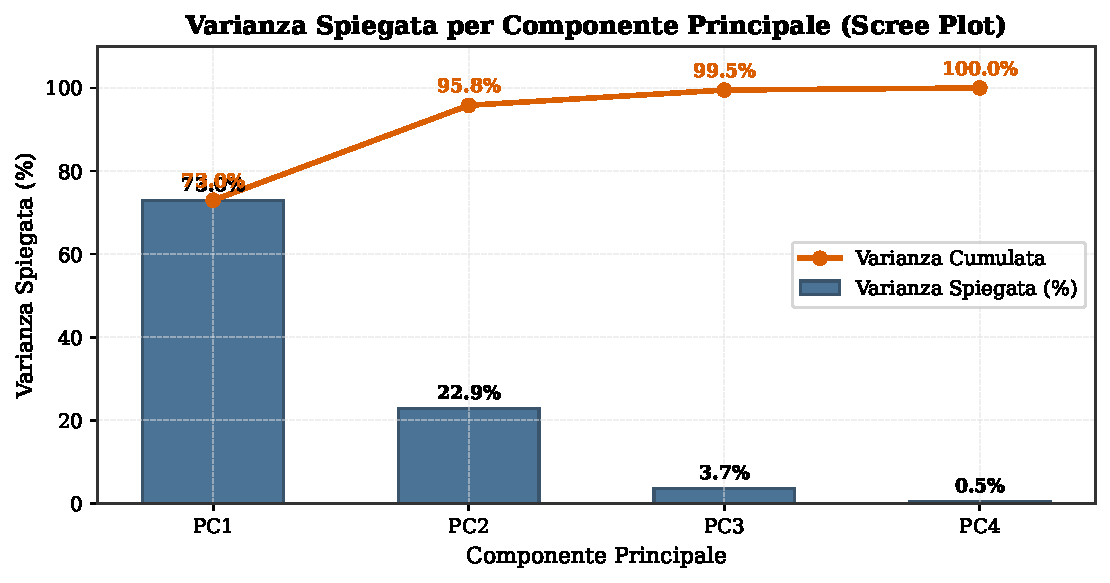
\includegraphics[width=0.82\textwidth]{pca_scree_plot.pdf}
    \caption{Scree plot degli autovalori e curva di varianza cumulativa spiegata.}
    \label{fig:dm-pca-scree}
\end{figure}

\subsubsection{Passo 5: Proiezione nel Nuovo Sottospazio}
La matrice finale proiettata $Z \in \mathbb{R}^{n \times k}$ nello spazio ridotto $k$-dimensionale si calcola mediante moltiplicazione matriciale:
\begin{equation}
    Z = C F
\end{equation}

In Figura~\ref{fig:dm-pca-2d} è visualizzata la proiezione dei campioni del dataset Iris sul piano bidimensionale definito dalle prime due componenti principali (PC1 e PC2), che catturano oltre il $95\%$ della varianza originaria complessiva.

\begin{figure}[htbp]
    \centering
    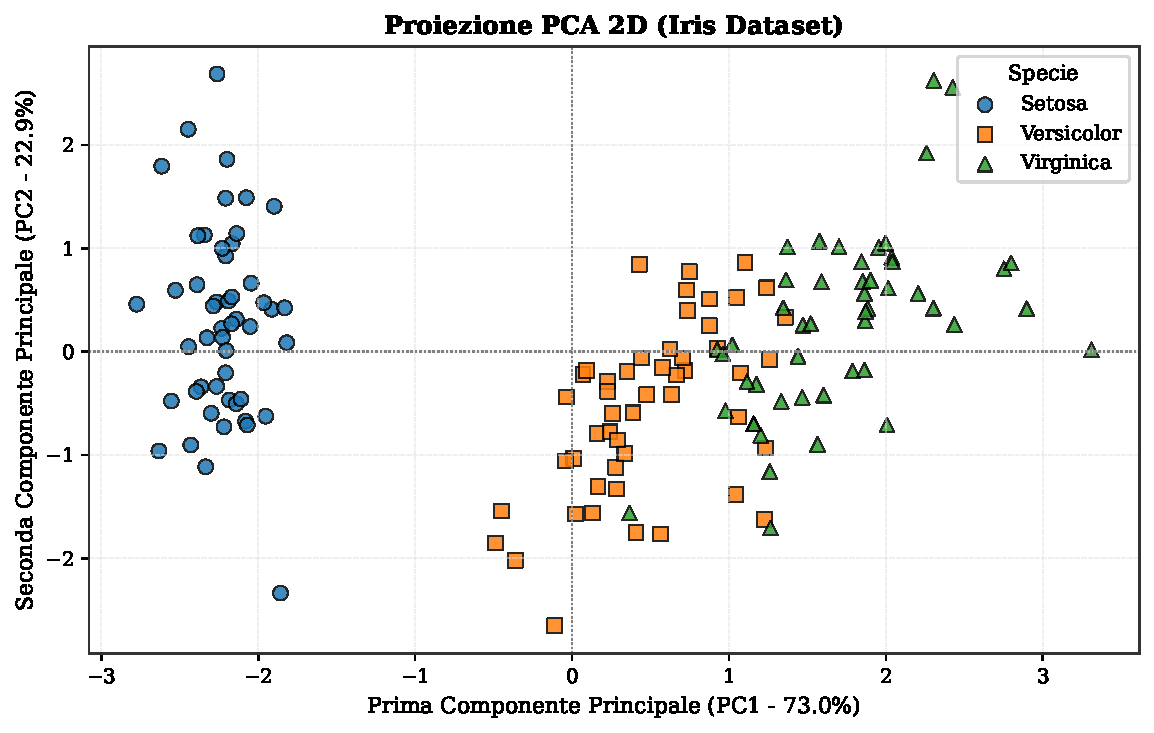
\includegraphics[width=0.88\textwidth]{pca_2d_projection.pdf}
    \caption{Proiezione bidimensionale dei campioni Iris lungo le prime due componenti principali.}
    \label{fig:dm-pca-2d}
\end{figure}

% ====================================================================
% SEZIONE 4.5: GESTIONE DEI VALORI MANCANTI
% ====================================================================
\section{Gestione dei Valori Mancanti}
\label{sec:dm-missing-values-handling}

Le strategie operative per il trattamento dei record incompleti comprendono:

\begin{enumerate}
    \item \textbf{Eliminazione Completa del Record (Listwise Deletion)}: Rimozione integrale di tutte le righe con almeno un campo nullo. Applicabile in sicurezza solo quando l'incidenza dei missing è trascurabile ($< 3-5\%$) e i dati mancano in modo puramente casuale (\textit{Missing Completely at Random - MCAR}); altrimenti introduce gravi distorsioni selettive.
    \item \textbf{Sostituzione con Indici di Tendenza Centrale}:
    \begin{itemize}[noitemsep]
        \item \textit{Media}: Per variabili numeriche simmetriche prive di outlier.
        \item \textit{Mediana}: Per variabili numeriche asimmetriche o in presenza di code pesanti.
        \item \textit{Moda}: Per attributi categorici qualitativi.
        \item \textit{Criticità}: Riduce artificialmente la varianza della feature e attenua l'intensità delle correlazioni con gli altri attributi.
    \end{itemize}
    \item \textbf{Imputazione Condizionale tramite Segmentazione}: Ripartizione dei campioni in cluster o classi omogenee sulla base delle feature complete e imputazione del valore mancante impiegando la media o mediana calcolata esclusivamente all'interno del rispettivo cluster.
    \item \textbf{Imputazione Predittiva Basata su Modelli}: Addestramento di un modello supervisionato (regressione lineare, $k$-NN, Random Forest) dove la variabile da stimare funge da target e gli attributi completi fungono da predittori.
\end{enumerate}

% ====================================================================
% SEZIONE 4.6: DISCRETIZZAZIONE E BINARIZZAZIONE
% ====================================================================
\section{Tecniche di Discretizzazione e Binarizzazione}
\label{sec:dm-discretization-binning}

La \textbf{discretizzazione} trasforma una variabile quantitativa continua in un attributo ordinale discreto, suddividendo il dominio continuo in un insieme finito di intervalli contigui (detti \textit{bin} o \textit{classi}).

\subsection{Discretizzazione Non Supervisionata}

\subsubsection{1. Natural Binning (Equal-Width Binning)}
Suddivide l'intervallo $[x_{\min}, x_{\max}]$ in $k$ classi aventi la medesima \textbf{ampiezza costante}:
\begin{equation}
    \delta = \frac{x_{\max} - x_{\min}}{k}
\end{equation}
L'$i$-esimo intervallo ($i = 0, \dots, k-1$) è delimitato da:
\begin{equation}
    I_i = \big[x_{\min} + i\delta,\, x_{\min} + (i+1)\delta\big)
\end{equation}

\begin{noteblock}{Esempio Numerico: Prezzo di 12 Birre}
Dato l'insieme di $N=12$ prezzi compresi tra $x_{\min}=100$ e $x_{\max}=160$, impostando $k=4$ classi otteniamo ampiezza $\delta = \frac{160-100}{4} = 15$. Gli intervalli risultano:
\begin{itemize}[noitemsep]
    \item Classe 1: $[100, 115) \to \{100, 110, 110\}$ (Conteggio: $3$)
    \item Classe 2: $[115, 130) \to \{120, 120, 125\}$ (Conteggio: $3$)
    \item Classe 3: $[130, 145) \to \{130, 130, 135, 140\}$ (Conteggio: $4$)
    \item Classe 4: $[145, 160] \to \{150, 160\}$ (Conteggio: $2$)
\end{itemize}
\end{noteblock}

\subsubsection{2. Equal-Frequency Binning (Equal-Depth Binning)}
Ordina i campioni in senso crescente e assegna a ciascun intervallo lo \textbf{stesso numero di osservazioni}:
\begin{equation}
    f = \frac{N}{k}
\end{equation}

Sugli stessi $12$ prezzi ordinati $\{100, 110, 110, 120, 120, 125, 130, 130, 135, 140, 150, 160\}$ con $k=4$, la frequenza per classe è $f = 12/4 = 3$:
\begin{itemize}[noitemsep]
    \item Classe 1: $\{100, 110, 110\}$
    \item Classe 2: $\{120, 120, 125\}$
    \item Classe 3: $\{130, 130, 135\}$
    \item Classe 4: $\{140, 150, 160\}$
\end{itemize}
Questo approccio uniforma la densità e mitiga l'impatto degli outlier, sebbene possa collocare valori contigui identici in classi distinte qualora cadano a cavallo della soglia.

\subsubsection{Formule per il Numero e l'Ampiezza Ottimale dei Bin}
Oltre alla Regola di Sturges, si utilizza la formulazione logaritmica decimale:
\begin{equation}
    C = 1 + \frac{10}{3} \log_{10}(N)
\end{equation}
Per ottimizzare direttamente l'ampiezza $h$ combinando variabilità e numerosità campionaria, si applica la \textbf{Regola di Scott (1979)}:
\begin{equation}
    h = \frac{3.5 \times s}{\sqrt[3]{N}}
\end{equation}
dove $s$ è la deviazione standard campionaria e $N$ la numerosità del dataset.

\subsection{Discretizzazione Supervisionata Basata sull'Entropia}

Quando è disponibile una variabile di classe target $Y \in \{c_1, \dots, c_m\}$, le soglie di taglio vengono ottimizzate per massimizzare la purezza informativa.
L'entropia di un insieme di campioni $S$ è data da:
\begin{equation}
    \text{Entropy}(S) = - \sum_{j=1}^m p_j \log_2(p_j)
\end{equation}
dove $p_j$ è la proporzione di istanze in $S$ appartenenti alla classe $c_j$. Se un punto di split $T$ partiziona $S$ nei sottoinsiemi $S_1$ ed $S_2$, l'entropia combinata pesata è:
\begin{equation}
    E(S, T) = \frac{|S_1|}{|S|} \text{Entropy}(S_1) + \frac{|S_2|}{|S|} \text{Entropy}(S_2)
\end{equation}
Il punto di split ottimale $T^*$ massimizza il guadagno informativo $\text{Gain}(S, T) = \text{Entropy}(S) - E(S, T)$.

\subsection{Binarizzazione (Encoding)}

Converte variabili qualitative con $m$ modalità in attributi binari $\{0, 1\}$:

\begin{itemize}
    \item \textbf{Codifica One-Hot (Asymmetric Binary Encoding)}: Alloca un indicatore binario dedicato per ciascuna modalità. Genera $m$ variabili asimmetriche ed evita di introdurre relazioni d'ordine artificiose:
    \begin{table}[htbp]
        \centering
        \small
        \begin{tabular}{lcccccc}
            \toprule
            \textbf{Valore Categorico} & \textbf{Codice Intero} & $x_1$ & $x_2$ & $x_3$ & $x_4$ & $x_5$ \\
            \midrule
            \textbf{awful} & 0 & 1 & 0 & 0 & 0 & 0 \\
            \textbf{poor}  & 1 & 0 & 1 & 0 & 0 & 0 \\
            \textbf{OK}    & 2 & 0 & 0 & 1 & 0 & 0 \\
            \textbf{good}  & 3 & 0 & 0 & 0 & 1 & 0 \\
            \textbf{great} & 4 & 0 & 0 & 0 & 0 & 1 \\
            \bottomrule
        \end{tabular}
        \caption{Esempio di codifica One-Hot per un attributo a 5 livelli qualitativi.}
        \label{tab:dm-one-hot}
    \end{table}

    \item \textbf{Codifica Binaria Compatta}: Mappa ciascuna modalità nella sua rappresentazione binaria posizionale numerica, richiedendo $n = \lceil \log_2(m) \rceil$ bit.
    \begin{table}[htbp]
        \centering
        \small
        \begin{tabular}{lcccc}
            \toprule
            \textbf{Valore Categorico} & \textbf{Codice Intero} & $x_1$ & $x_2$ & $x_3$ \\
            \midrule
            \textbf{awful} & 0 & 0 & 0 & 0 \\
            \textbf{poor}  & 1 & 0 & 0 & 1 \\
            \textbf{OK}    & 2 & 0 & 1 & 0 \\
            \textbf{good}  & 3 & 0 & 1 & 1 \\
            \textbf{great} & 4 & 1 & 0 & 0 \\
            \bottomrule
        \end{tabular}
        \caption{Codifica binaria compatta su 3 bit per 5 livelli categorici.}
        \label{tab:dm-compact-binary}
    \end{table}
    \textit{Criticità}: Induce correlazioni fittizie tra i singoli bit privi di riscontro empirico nel fenomeno reale.
\end{itemize}

% ====================================================================
% SEZIONE 4.7: TRASFORMAZIONI FUNZIONALI
% ====================================================================
\section{Trasformazioni Funzionali di Attributi e Stabilizzazione della Varianza}
\label{sec:dm-functional-transformations}

Una \textbf{trasformazione funzionale} applica una funzione $T$ continua e strettamente monotona a ciascun valore di un attributo $X$: $Y = T(X)$.
\begin{itemize}[noitemsep]
    \item \textbf{Stabilizzazione della varianza}: Rende omogenea la dispersione lungo tutto il dominio (\textit{omoschedasticità}).
    \item \textbf{Normalizzazione della forma}: Riconduce code pesanti o asimmetrie a distribuzioni approssimativamente normali.
    \item \textbf{Linearizzazione delle relazioni}: Rende lineari dipendenze polinomiali o esponenziali.
\end{itemize}

\subsection{Famiglia delle Trasformazioni Esponenziali e Logaritmiche}
La trasformazione parametrica generale è definita come:
\begin{equation}
    T_p(x) = \begin{cases}
        a x^p + b & \text{se } p \neq 0 \\
        c \log(x) + d & \text{se } p = 0
    \end{cases}
\end{equation}
con $x > 0$.
\begin{itemize}
    \item \textbf{Trasformazione Lineare ($p = 1$)}: Modifica unicamente origine e scala (es. euro in lire con $a=1936.27, b=0$; gradi Fahrenheit in Celsius con $a=5/9, b=-160/9$).
    \item \textbf{Trasformazione Logaritmica ($p = 0$)}: $T(x) = c\log(x) + d$. Comprime i valori elevati ed espande la scala dei valori piccoli, contrastando l'asimmetria positiva destra.
\end{itemize}

\begin{table}[htbp]
    \centering
    \small
    \begin{tabular}{llcc}
        \toprule
        \textbf{Bar} & \textbf{Birra} & \textbf{Gain Originario ($X$)} & \textbf{Gain Trasformato $\log_{10}(X)$} \\
        \midrule
        A & Bud   & 20    & 1.3010 \\
        A & Becks & 10000 & 4.0000 \\
        C & Bud   & 300   & 2.4771 \\
        D & Bud   & 400   & 2.6021 \\
        D & Becks & 5     & 0.6990 \\
        E & Becks & 120   & 2.0792 \\
        E & Bud   & 120   & 2.0792 \\
        F & Bud   & 11000 & 4.0414 \\
        G & Bud   & 1300  & 3.1139 \\
        H & Bud   & 3200  & 3.5051 \\
        H & Becks & 1000  & 3.0000 \\
        I & Bud   & 135   & 2.1303 \\
        \bottomrule
    \end{tabular}
    \caption{Campione di 12 osservazioni di profitto (Gain) prima e dopo trasformazione logaritmica.}
    \label{tab:dm-log-transform-sample}
\end{table}

\begin{table}[htbp]
    \centering
    \small
    \begin{tabularx}{\textwidth}{Xcc}
        \toprule
        \textbf{Parametro Statistico} & \textbf{Scala Originaria ($X$)} & \textbf{Scala Logaritmica ($Y = \log_{10} X$)} \\
        \midrule
        \textbf{Media Aritmetica} & 2481.82 & 2.5956 \\
        \textbf{Deviazione Standard} & 4079.02 & 1.0651 \\
        \textbf{Minimo} & 5 & 0.6990 \\
        \textbf{$1^\circ$ Quartile ($Q_1$)} & 120 & 2.0792 \\
        \textbf{Mediana ($Q_2$)} & 400 & 2.6021 \\
        \textbf{$3^\circ$ Quartile ($Q_3$)} & 2250 & 3.3095 \\
        \textbf{Massimo} & 11000 & 4.0414 \\
        \bottomrule
    \end{tabularx}
    \caption{Indicatori statistici descrittivi prima e dopo la trasformazione logaritmica.}
    \label{tab:dm-log-transform-stats}
\end{table}

Nella scala originaria la deviazione standard ($4079.02$) eccede abbondantemente la media ($2481.82$), trascinata dai picchi a $10000$ e $11000$. Dopo la conversione in $\log_{10}$, media ($2.5956$) e mediana ($2.6021$) coincidono quasi perfettamente, ripristinando la simmetria.

\subsection{Altre Trasformazioni di Stabilizzazione}
\begin{itemize}[noitemsep]
    \item \textbf{Radice Quadrata ($p = 1/2$)}: $T(x) = \sqrt{x}$. Stabilizza la varianza nei dati di conteggio poissoniani ($\sigma^2 = \mu$).
    \item \textbf{Reciproca ($p = -1$)}: $T(x) = 1/x$. Utilizzata quando la varianza cresce in modo quadratico o superlineare rispetto alla media.
\end{itemize}

% ====================================================================
% SEZIONE 4.8: ALGORITMI DI NORMALIZZAZIONE
% ====================================================================
\section{Algoritmi di Normalizzazione}
\label{sec:dm-normalization-algorithms}

La normalizzazione riconduce attributi misurati su scale numeriche disomogenee all'interno di intervalli standard comparabili, scongiurando il dominio distorto di feature con valori numerici elevati negli algoritmi basati sulle distanze metriche ($k$-NN, K-Means, SVM, reti neurali).

\subsection{Normalizzazione Min-Max}
Mappa linearmente l'intervallo originario $[\min_A, \max_A]$ nell'intervallo target $[\text{new\_min}_A, \text{new\_max}_A]$ (frequentemente $[0, 1]$):
\begin{equation}
    v' = \frac{v - \min_A}{\max_A - \min_A} \big(\text{new\_max}_A - \text{new\_min}_A\big) + \text{new\_min}_A
\end{equation}
Preserva esattamente le relazioni lineari originarie, ma risulta sensibile a outlier estremi che possono comprimere i valori ordinari in un sottointervallo minuscolo.

\subsection{Standardizzazione Z-Score}
Riconduce la variabile ad avere \textbf{media nulla e varianza unitaria}:
\begin{equation}
    v' = \frac{v - \bar{x}_A}{s_A}
\end{equation}
dove $\bar{x}_A$ è la media campionaria e $s_A$ la deviazione standard campionaria. È l'approccio raccomandato per distribuzioni approssimativamente normali e resiste meglio alla presenza di valori sparsi nelle code.

\subsection{Normalizzazione per Scalamento Decimale (Decimal Scaling)}
Sposta la virgola decimale dividendo per una potenza di $10$:
\begin{equation}
    v' = \frac{v}{10^j}
\end{equation}
dove $j$ è il minimo intero positivo tale che:
\begin{equation}
    \max(|v'|) < 1 \iff 10^{j-1} \le \max(|v|) < 10^j
\end{equation}

\begin{noteblock}{Esempio Numerico di Decimal Scaling}
Dato il vettore $V = \{-10,\, 201,\, 301,\, -401,\, 501,\, 601,\, 701\}$:
\begin{enumerate}
    \item Il massimo in valore assoluto è $m = \max(|v|) = 701$.
    \item Il minimo intero $j$ tale che $10^j > 701$ è $j=3$ ($10^3 = 1000$).
    \item Dividendo per $1000$ si ottiene:
    \begin{equation}
        V' = \{-0.01,\, 0.201,\, 0.301,\, -0.401,\, 0.501,\, 0.601,\, 0.701\}
    \end{equation}
    Tutti i valori trasformati appartengono rigidamente all'intervallo aperto $(-1, +1)$.
\end{enumerate}
\end{noteblock}

% ====================================================================
% SEZIONE 4.9: TRATTAMENTO UNIVARIATO DEGLI OUTLIER
% ====================================================================
\section{Trattamento Univariato degli Outlier}
\label{sec:dm-univariate-outlier-treatment}

Richiamando i criteri diagnostici fondati su Boxplot, Range Interquartilico (IQR) e Z-Score formalizzati nel Capitolo~\ref{chap:dm-data-understanding-multivariate-outliers} (\autoref{sec:dm-outlier-detection-taxonomy}), la fase di \textit{Data Preparation} definisce le regole operative per neutralizzare l'influenza distorsiva dei valori anomali isolati senza necessariamente scartare l'intero record:

\begin{figure}[htbp]
    \centering
    \begin{tikzpicture}[
        ruleCard/.style={draw=navy!80!black, fill=navy!6, rounded corners=6pt, thick, font=\footnotesize, align=left, text width=6.0cm, minimum height=3.2cm, inner sep=6pt},
        arrowStyle/.style={-Stealth, thick, draw=navy!85!black}
    ]
        % Root
        \node[rectangle, rounded corners=6pt, draw=purple!85!black, fill=purple!12, very thick, font=\small\bfseries, align=center, text width=10.0cm, inner sep=6pt] (root) at (0, 2.7) {
            RILEVAMENTO E SOSTITUZIONE OUTLIER\\[2pt]
            \footnotesize \normalfont Criteri univariati per l'identificazione e il trattamento
        };
        
        % Ramo Sinistro: Tukey
        \node[ruleCard, anchor=north] (tukeyCol) at (-3.6, 1.1) {
            \textbf{Criterio IQR (Tukey)}\\[3pt]
            $L = Q_1 - 1.5\,\text{IQR},\quad U = Q_3 + 1.5\,\text{IQR}$\\[2pt]
            Outlier se: $x < L \lor x > U$\\[4pt]
            \textbf{Strategie di Sostituzione}:\\[2pt]
            1. \textbf{Winsorizzazione}: Assegna $L$ o $U$\\
            2. \textbf{Imputazione}: Assegna Mediana
        };
        
        % Ramo Destro: Z-score
        \node[ruleCard, anchor=north] (zscoreCol) at (3.6, 1.1) {
            \textbf{Criterio Z-Score}\\[3pt]
            Standardizzazione: $z = (x - \bar{x}) / s$\\[2pt]
            Outlier se: $|z| > 3.29$ (coda $0.1\%$)\\[4pt]
            \textbf{Strategie di Sostituzione}:\\[2pt]
            1. \textbf{Troncamento}: Soglia $z = \pm 3.0$\\
            2. \textbf{Imputazione}: Assegna Media ($z = 0$)
        };
        
        \coordinate (split) at (0, 1.65);
        \draw[thick, draw=navy!85!black] (root.south) -- (split);
        \draw[arrowStyle] (split) -| (tukeyCol.north);
        \draw[arrowStyle] (split) -| (zscoreCol.north);
    \end{tikzpicture}
    \caption{Quadro decisionale per l'identificazione e la sostituzione univariata degli outlier.}
    \label{fig:dm-outlier-replacement-rules}
\end{figure}

\subsection{Trattamento Basato sul Range Interquartilico (Tukey)}
Individuate le recinzioni di Tukey $[L, U] = [Q_1 - 1.5\,\text{IQR}, \, Q_3 + 1.5\,\text{IQR}]$, le opzioni di bonifica per i valori esterni $x \notin [L, U]$ prevedono:
\begin{itemize}
    \item \textbf{Winsorizzazione (Sostituzione al bordo)}: Si imposta $x' = L$ se $x < L$, e $x' = U$ se $x > U$. Questa trasformazione preserva la monotonicità ordinale e la numerosità campionaria originale, annullando la magnitudo distorsiva del picco estremo;
    \item \textbf{Imputazione con la Mediana}: Si rimpiazza il valore estremo con la mediana calcolata sul sottoinsieme dei dati regolari interni all'intervallo $[L, U]$.
\end{itemize}

\subsection{Trattamento Basato sullo Z-Score}
Per attributi a distribuzione approssimativamente normale con anomalie identificate dalla condizione $|z| > 3.29$, si adottano due strategie di sostituzione:
\begin{enumerate}
    \item \textbf{Troncamento a $3\sigma$ (Clamping)}: Il valore estremo viene convertito nel valore corrispondente al punto di soglia $z = \pm 3.0$ ($x' = \bar{x} \pm 3.0\,s$). Questa scelta riconduce il record entro un intervallo plausibile senza cancellare l'informazione che l'osservazione apparteneva all'estremo della coda;
    \item \textbf{Imputazione con la Media Campionaria}: Il valore anomalo viene rimpiazzato con il baricentro $z = 0$, corrispondente alla media campionaria originaria $\bar{x}$.
\end{enumerate}

\chapter{Laboratorio Python: Data Understanding e Data Preparation}
\label{chap:dm-python-lab-du-dp}

In questo capitolo viene presentata la trasposizione computazionale delle metodologie teoriche di Data Understanding (DU) e Data Preparation (DP), facendo riferimento all'attività di laboratorio svolta con lo stack scientifico di Python (\texttt{numpy}, \texttt{pandas}, \texttt{scipy}, \texttt{matplotlib}, \texttt{seaborn} e \texttt{scikit-learn}).

Il laboratorio impiega il dataset \textbf{Tips} (arricchito con la tabella \textbf{Tips\_Age}), relativo alle abitudini di spesa e di mancia dei clienti di un ristorante, per illustrare l'intero flusso operativo: dall'ingestione e integrazione dei dati, alla diagnosi e imputazione dei valori mancanti, fino all'ingegnerizzazione delle feature, normalizzazione e riduzione dimensionale con PCA e $t$-SNE.

\begin{noteblock}{Ambiente Interattivo e Riproducibilità del Laboratorio}
    Tutti gli esempi, le pipeline di trasformazione e i grafici presentati in questo capitolo sono riproducibili ed eseguibili interattivamente tramite i notebook Jupyter inclusi nella cartella \texttt{Data-Mining/notebooks/}.
    
    \textbf{Avvio rapido con Docker}:
    \begin{itemize}[noitemsep]
        \item Da terminale (nella radice del progetto): \texttt{docker compose up jupyter}
        \item Oppure con doppio clic su Windows: \texttt{scripts/start-jupyter.cmd}
        \item Interfaccia web: \href{http://localhost:8888/lab}{\texttt{http://localhost:8888/lab}} (senza password né token).
    \end{itemize}
    Per eseguire direttamente gli script senza interfaccia grafica da riga di comando:
    \begin{itemize}[noitemsep]
        \item \texttt{docker compose run --rm app python3 Data-Mining/notebooks/generate\_dispensa\_figures.py}
    \end{itemize}
\end{noteblock}

% ====================================================================
% SEZIONE 5.1: AMBIENTE, INGESTIONE E DATA INTEGRATION
% ====================================================================
\section{Ambiente di Lavoro, Ingestione e Data Integration}
\label{sec:dm-lab-ingestion-integration}

\begin{remark}[Riferimento al Notebook Interattivo]
    Il codice delle sezioni \ref{sec:dm-lab-ingestion-integration}, \ref{sec:dm-lab-missing-values} e \ref{sec:dm-lab-multivariate-exploration} corrisponde al notebook Jupyter interattivo \href{http://localhost:8888/lab/tree/notebooks/1_basics_and_understanding.ipynb}{\textbf{Notebook 1 (Data Understanding)}} (file \texttt{1\_basics\_and\_} \texttt{understanding.ipynb}).
\end{remark}

Lo stack software fondamentale per l'analisi esplorativa dei dati in Python comprende le seguenti librerie:

\begin{lstlisting}[language=Python, style=code]
import numpy as np
import pandas as pd
import scipy.stats as stats
import matplotlib.pyplot as plt
import seaborn as sns
from sklearn.impute import SimpleImputer, KNNImputer
from sklearn.preprocessing import StandardScaler, MinMaxScaler, KBinsDiscretizer, OneHotEncoder, TargetEncoder
from sklearn.decomposition import PCA
from sklearn.manifold import TSNE
\end{lstlisting}

\subsection{Caricamento e Ispezione Strutturale}

Il dataset principale viene acquisito tramite file delimitato da tabulazione (\texttt{tsv}) impostando l'indice sulla prima colonna:

\begin{lstlisting}[language=Python, style=code]
tips = pd.read_csv('tips.csv', sep='\t', index_col=0)
print(tips.head())
tips.info()
\end{lstlisting}

Il dataset contiene inizialmente $244$ osservazioni e $7$ colonne: \texttt{total\_bill} (importo totale del conto), \texttt{tip} (mancia), \texttt{sex} (genere del pagante), \texttt{smoker} (presenza di fumatori al tavolo), \texttt{day} (giorno della settimana), \texttt{time} (pranzo o cena), \texttt{size} (numero di coperti al tavolo).

\subsection{Data Integration e Join Relazionale}

Nel laboratorio, l'età dei clienti è memorizzata in una sorgente secondaria (\texttt{tips\_age.csv}). L'integrazione delle due tabelle avviene tramite una join sull'identificativo primario \texttt{ID}:

\begin{lstlisting}[language=Python, style=code]
tips_age = pd.read_csv('tips_age.csv', sep='\t', index_col=0)
df = tips.join(tips_age, on='ID')
# Rimozione di eventuali colonne ridondanti generate dalla sorgente
df = df.drop(columns=['gender'], errors='ignore')
\end{lstlisting}

\subsection{Rilevamento e Rimozione di Record Duplicati}

L'ispezione delle righe duplicate richiede la verifica dell'uguaglianza tra tutti gli attributi del record:

\begin{lstlisting}[language=Python, style=code]
# Visualizzazione di tutti i duplicati (tutte le copie)
duplicated_rows = df[df.duplicated(keep=False)]
print(f"Righe duplicate rilevate: {len(duplicated_rows)}")

# Rimozione mantenendo la prima occorrenza
df = df.drop_duplicates()
\end{lstlisting}

\subsection{Bonifica di Valori Non Validi e Cast di Tipo}

Spesso i dati contengono errori di trascrizione o stringhe non valide inserite al posto di campi numerici (ad esempio il valore fittizio \texttt{'aaaaa'} nella colonna \texttt{total\_bill}). Ciò costringe Pandas a tipizzare la colonna come generico tipo \texttt{object}. La bonifica avviene mediante sostituzione puntuale e conversione esplicita di tipo:

\begin{lstlisting}[language=Python, style=code]
# Sostituzione della stringa anomala con zero o NaN
df["total_bill"] = df["total_bill"].replace("aaaaa", np.nan)

# Cast esplicito a float numerico
df["total_bill"] = pd.to_numeric(df["total_bill"])
\end{lstlisting}

% ====================================================================
% SEZIONE 5.2: DIAGNOSI E IMPUTAZIONE DEI VALORI MANCANTI
% ====================================================================
\section{Diagnosi e Imputazione dei Valori Mancanti}
\label{sec:dm-lab-missing-values}

\subsection{Audit dei Missing Values}

Il conteggio dei valori mancanti (\texttt{NaN}) per ciascun attributo si ottiene combinando \texttt{isnull()} e \texttt{sum()}:

\begin{lstlisting}[language=Python, style=code]
# Riepilogo dei valori nulli per colonna
null_counts = df.isnull().sum()
print(null_counts[null_counts > 0])

# Selezione dei soli record incompleti
incomplete_records = df[df.isnull().any(axis=1)]
\end{lstlisting}

\subsection{Strategie di Rimozione vs Imputazione Statistica}

\begin{itemize}
    \item \textbf{Listwise Deletion}: Eliminazione integrale di tutti i record con almeno un valore nullo:
\begin{lstlisting}[language=Python, style=code]
df_cleaned = df.dropna()
\end{lstlisting}
    \item \textbf{Imputazione con la Mediana Condizionale}: Quando l'attributo \texttt{age} presenta valori mancanti o codificati con la convenzione sentinella $0$, l'imputazione mediante la mediana calcolata sull'intero dataset potrebbe appiattire la variabilità tra fasce orarie distinte (\textit{Lunch} vs \textit{Dinner}). Si esegue pertanto un'imputazione stratificata:
\begin{lstlisting}[language=Python, style=code]
df['age'] = df['age'].replace(0, np.nan)
# Imputa con la mediana di gruppo calcolata sulla fascia oraria (time)
df['age'] = df['age'].fillna(df.groupby('time')['age'].transform('median'))
\end{lstlisting}
\end{itemize}

\subsection{Imputazione Avanzata con Scikit-Learn}

Il modulo \texttt{sklearn.impute} mette a disposizione trasformatori integrabili nelle pipeline di machine learning:

\begin{lstlisting}[language=Python, style=code]
# 1. SimpleImputer per feature numeriche (media o mediana)
imp_mean = SimpleImputer(strategy='mean')
df['tip'] = imp_mean.fit_transform(df[['tip']])

# 2. SimpleImputer per feature categoriche (moda/frequenza massima)
imp_mode = SimpleImputer(strategy='most_frequent')
df['smoker'] = imp_mode.fit_transform(df[['smoker']]).ravel()

# 3. KNNImputer (imputazione multivariata basata su k-Nearest Neighbors)
knn_imp = KNNImputer(n_neighbors=2, weights='distance')
num_cols = ['total_bill', 'tip', 'size', 'age']
df[num_cols] = knn_imp.fit_transform(df[num_cols])
\end{lstlisting}

% ====================================================================
% SEZIONE 5.3: ESPLORAZIONE MULTIVARIATA E CORRELAZIONE
% ====================================================================
\section{Esplorazione Multivariata e Analisi di Correlazione}
\label{sec:dm-lab-multivariate-exploration}

\subsection{Tabelle di Contingenza e Distribuzioni Condizionate}

Per studiare le associazioni tra variabili categoriche si utilizzano tabelle di contingenza normalizzate (\textit{cross-tabulation}):

\begin{lstlisting}[language=Python, style=code]
# Tabella di frequenza congiunta tra genere e abitudine al fumo
smoker_xt = pd.crosstab(df['smoker'], df['sex'])

# Normalizzazione per riga (proporzioni percentuali)
smoker_pct = smoker_xt.div(smoker_xt.sum(1).astype(float), axis=0)
smoker_pct.plot(kind='bar', stacked=False, title='Genere per Categoria Fumatore')
plt.ylabel('Frequenza Relativa')
plt.show()
\end{lstlisting}

\subsection{Matrici di Correlazione e Heatmap}

Pandas consente di stimare simultaneamente i coefficienti di correlazione lineare (Pearson) e di rango (Spearman, Kendall) sui soli attributi numerici:

\begin{lstlisting}[language=Python, style=code]
# Calcolo della matrice di correlazione di Pearson
corr_pearson = df.corr(numeric_only=True, method='pearson')

# Calcolo con il coefficiente di Spearman (monotonia robusta)
corr_spearman = df.corr(numeric_only=True, method='spearman')

# Visualizzazione grafica tramite heatmap con annotazioni numeriche
plt.figure(figsize=(8, 6))
sns.heatmap(corr_pearson, annot=True, cmap='coolwarm', fmt='.2f', vmin=-1, vmax=1)
plt.title('Matrice di Correlazione di Pearson (Dataset Tips)')
plt.show()
\end{lstlisting}

\subsection{Scatter Matrix e Pairplot}

L'ispezione visiva incrociata delle relazioni bivariate si realizza tramite \texttt{scatter\_matrix} o Seaborn \texttt{pairplot}:

\begin{lstlisting}[language=Python, style=code]
# Scatter Matrix di Pandas
pd.plotting.scatter_matrix(df[['total_bill', 'tip', 'size', 'age']], figsize=(9, 9), diagonal='kde')
plt.show()

# Pairplot con codice colore basato sul momento del pasto (time)
sns.pairplot(df, vars=['total_bill', 'tip', 'size'], hue='time', palette='Dark2')
plt.show()
\end{lstlisting}

\subsection{Feature Engineering: Costruzione di Indicatori di Dominio}

La conoscenza del dominio consente di combinare variabili grezze per sintetizzare nuovi attributi ad alto valore interpretativo:

\begin{lstlisting}[language=Python, style=code]
# 1. Percentuale effettiva di mancia rispetto al conto
df['tip_ratio'] = df['tip'] / df['total_bill']

# 2. Spesa media per persona (Bill Per Person - BPP)
df['bpp'] = df['total_bill'] / df['size']

# Ispezione con Boxplot condizionato per genere
df.boxplot(column=['bpp'], by='sex')
plt.title('Spesa Media per Persona per Genere')
plt.suptitle('')
plt.show()
\end{lstlisting}

% ====================================================================
% SEZIONE 5.4: FEATURE TRANSFORMATION E ENCODING
% ====================================================================
\section{Feature Transformation, Discretizzazione e Encoding}
\label{sec:dm-lab-transformation-encoding}

\begin{remark}[Riferimento al Notebook Interattivo]
    Il codice delle sezioni \ref{sec:dm-lab-transformation-encoding} e \ref{sec:dm-lab-dimensionality-reduction} corrisponde al notebook Jupyter interattivo \href{http://localhost:8888/lab/tree/notebooks/2_feature_engineering_and_data_representation.ipynb}{\textbf{Notebook 2 (Feature Engineering)}}:
    \begin{center}
        \small \href{http://localhost:8888/lab/tree/notebooks/2_feature_engineering_and_data_representation.ipynb}{\texttt{2\_feature\_engineering\_and\_data\_representation.ipynb}}
    \end{center}
\end{remark}

\subsection{Discretizzazione con KBinsDiscretizer}

La libreria Scikit-Learn fornisce \texttt{KBinsDiscretizer} per convertire variabili continue in classi ordinali discrete secondo tre strategie:

\begin{lstlisting}[language=Python, style=code]
# Discretizzazione a 4 intervalli con strategie diverse
disc_uniform = KBinsDiscretizer(n_bins=4, encode='ordinal', strategy='uniform')    # Equal-Width
disc_quantile = KBinsDiscretizer(n_bins=4, encode='ordinal', strategy='quantile')  # Equal-Frequency
disc_kmeans = KBinsDiscretizer(n_bins=4, encode='ordinal', strategy='kmeans')      # Basata su Cluster

df['total_bill_bins'] = disc_uniform.fit_transform(df[['total_bill']])
print(df['total_bill_bins'].value_counts())
\end{lstlisting}

\subsection{Normalizzazione dei Dati: StandardScaler vs MinMaxScaler}

\begin{itemize}
    \item \textbf{StandardScaler}: Trasforma la feature per avere media zero e deviazione standard unitaria ($\mu = 0, \sigma = 1$).
    \item \textbf{MinMaxScaler}: Riscala linearmente l'intervallo originario entro $[0, 1]$.
\end{itemize}

\begin{lstlisting}[language=Python, style=code]
num_cols = ['total_bill', 'tip', 'age']

# Standardizzazione Z-Score
scaler_std = StandardScaler()
df_standardized = df.copy()
df_standardized[num_cols] = scaler_std.fit_transform(df[num_cols])

# Normalizzazione Min-Max
scaler_minmax = MinMaxScaler()
df_normalized = df.copy()
df_normalized[num_cols] = scaler_minmax.fit_transform(df[num_cols])

# Ripristino dei valori originari tramite trasformazione inversa
df_recovered = scaler_minmax.inverse_transform(df_normalized[num_cols])
\end{lstlisting}

\subsection{Codifica di Variabili Categoriche: One-Hot vs Target Encoding}

\begin{lstlisting}[language=Python, style=code]
# 1. One-Hot Encoding (evita di creare ordinalita fittizia)
ohe = OneHotEncoder(handle_unknown='ignore', sparse_output=False)
encoded_days = ohe.fit_transform(df[['day']])
encoded_df = pd.DataFrame(encoded_days, columns=ohe.get_feature_names_out(['day']))

# 2. Target Encoding (sostituisce la categoria con la media della target)
target_enc = TargetEncoder(smooth='auto')
# Codifica 'day' in base all'importo medio della mancia 'tip'
df['day_target_encoded'] = target_enc.fit_transform(df[['day']], df['tip'])
\end{lstlisting}

% ====================================================================
% SEZIONE 5.5: RIDUZIONE DIMENSIONALE: PCA E T-SNE
% ====================================================================
\section{Riduzione Dimensionale: PCA e $t$-SNE}
\label{sec:dm-lab-dimensionality-reduction}

\subsection{Principal Component Analysis (PCA)}

Prima di applicare la PCA è indispensabile standardizzare le feature continue affinché attributi con varianze ampie non dominino la decomposizione spettrale:

\begin{lstlisting}[language=Python, style=code]
# Selezione attributi quantitativi
X = df[['total_bill', 'tip', 'size', 'age', 'tip_ratio', 'bpp']].dropna()
X_scaled = StandardScaler().fit_transform(X)

# Esecuzione della PCA
pca = PCA()
X_pca = pca.fit_transform(X_scaled)

# Autovalori (quota di varianza spiegata per componente)
eigenvalues = pca.explained_variance_
# Percentuale di varianza spiegata
explained_var_ratio = pca.explained_variance_ratio_
# Varianza cumulata
cumulative_var = np.cumsum(explained_var_ratio)
\end{lstlisting}

\subsubsection{Costruzione dello Scree Plot}
Lo Scree Plot consente di individuare visivamente il "gomito" (\textit{elbow}) oltre il quale le componenti spiegano quote trascurabili di varianza:

\begin{lstlisting}[language=Python, style=code]
plt.figure(figsize=(8, 4))
plt.plot(range(1, len(eigenvalues) + 1), eigenvalues, 'o-', color='navy', label='Autovalori singoli')
plt.title('Scree Plot degli Autovalori (PCA)')
plt.xlabel('Numero Componente Principale')
plt.ylabel('Autovalore (Varianza spiegata)')
plt.grid(True, linestyle='--', alpha=0.5)
plt.legend()
plt.show()
\end{lstlisting}

\subsection{Proiezione Non Lineare con $t$-SNE}

Il \textbf{$t$-Distributed Stochastic Neighbor Embedding ($t$-SNE)} è una tecnica non supervisionata non lineare specificamente progettata per preservare le strutture di vicinato locale nei dati ad alta dimensionalità:

\begin{lstlisting}[language=Python, style=code]
tsne = TSNE(
    n_components=2,
    perplexity=30,      # Equilibrio tra granularita locale e globale (tipicamente 5-50)
    learning_rate=200,  # Passo di ottimizzazione della discesa del gradiente
    max_iter=1000,      # Iterazioni di minimizzazione della divergenza KL
    random_state=42
)
X_tsne = tsne.fit_transform(X_scaled)
\end{lstlisting}

\subsection{Confronto Metodologico tra PCA e $t$-SNE}

\begin{table}[htbp]
    \centering
    \small
    \begin{tabularx}{\textwidth}{lXX}
        \toprule
        \textbf{Caratteristica} & \textbf{PCA (Principal Component Analysis)} & \textbf{$t$-SNE ($t$-Distributed SNE)} \\
        \midrule
        \textbf{Tipologia} & Lineare, globale, deterministica. & Non lineare, locale, probabilistica/stocastica. \\
        \addlinespace
        \textbf{Funzione Obiettivo} & Massimizza la varianza globale proiettata (decomposizione agli autovalori). & Minimizza la divergenza di Kullback-Leibler tra distribuzioni di probabilità di vicinato. \\
        \addlinespace
        \textbf{Interpretabilità} & Gli assi rappresentano combinazioni lineari degli attributi (pesi/loading noti). & Gli assi non hanno significato fisico; contano solo le distanze relative tra punti. \\
        \addlinespace
        \textbf{Distanze Lontane} & Preserva fedelmente le distanze euclidee su larga scala. & Non preserva le distanze globali tra cluster distanti (la grandezza dei cluster non riflette la densità originaria). \\
        \addlinespace
        \textbf{Uso Tipico} & Riduzione preliminare di feature per modelli predittivi, compressione, eliminazione di collinearità. & Visualizzazione esplorativa avanzata e separazione visiva di cluster complessi (2D/3D). \\
        \bottomrule
    \end{tabularx}
    \caption{Confronto metodologico tra PCA e $t$-SNE nell'analisi dei dati.}
    \label{tab:dm-pca-vs-tsne}
\end{table}

\begin{lstlisting}[language=Python, style=code]
# Visualizzazione comparata delle due proiezioni bidimensionali
fig, (ax1, ax2) = plt.subplots(1, 2, figsize=(14, 5))

# Scatter PCA
ax1.scatter(X_pca[:, 0], X_pca[:, 1], c='navy', alpha=0.7, edgecolors='k')
ax1.set_title('Proiezione Lineare PCA (PC1 vs PC2)')
ax1.set_xlabel('Prima Componente Principale')
ax1.set_ylabel('Seconda Componente Principale')
ax1.grid(True, linestyle='--', alpha=0.5)

# Scatter t-SNE
ax2.scatter(X_tsne[:, 0], X_tsne[:, 1], c='crimson', alpha=0.7, edgecolors='k')
ax2.set_title('Proiezione Non Lineare t-SNE')
ax2.set_xlabel('Dimensione t-SNE 1')
ax2.set_ylabel('Dimensione t-SNE 2')
ax2.grid(True, linestyle='--', alpha=0.5)

plt.tight_layout()
plt.show()
\end{lstlisting}

\chapter{Misure di Prossimità, Teoria dell'Informazione e Cluster Analysis}
\label{chap:dm-similarity-clustering-foundations}

In questo capitolo vengono presentati i fondamenti matematici e concettuali su cui poggiano le discipline di apprendimento non supervisionato e basato su istanze nel Data Mining:
\begin{enumerate}[noitemsep]
    \item La quantificazione analitica della \textbf{vicinanza, distanza e similarità} tra oggetti descritti da attributi eterogenei e continui;
    \item Gli strumenti formali della \textbf{Teoria dell'Informazione di Shannon} (entropia ed informazione mutua) per valutare l'incertezza e la dipendenza non lineare;
    \item I principi generali, le tassonomie e le formulazioni geometriche della \textbf{Cluster Analysis}.
\end{enumerate}

% ====================================================================
% SEZIONE 6.1: FONDAMENTI DI PROSSIMITÀ, SIMILARITÀ E DISSIMILARITÀ
% ====================================================================
\section{Fondamenti di Similarità, Dissimilarità e Prossimità}
\label{sec:dm-foundations-proximity}

Nelle discipline di Data Mining, Machine Learning e Information Retrieval, il confronto tra coppie di entità informative costituisce il nucleo operativo di molteplici paradigmi analitici: dalla classificazione supervisionata mediante istanze vicine ($k$-Nearest Neighbors), all'estrazione di cluster naturali, fino alla stima di densità e anomalie.

\begin{figure}[htbp]
\centering
\begin{tikzpicture}[
    conceptBox/.style={rectangle, rounded corners=5pt, draw=navy!85!black, fill=navy!8, thick, font=\footnotesize, align=center, text width=5.6cm, inner sep=6pt},
    rootBox/.style={rectangle, rounded corners=6pt, draw=purple!85!black, fill=purple!12, very thick, font=\small\bfseries, align=center, text width=10.0cm, inner sep=6pt},
    arrowStyle/.style={-Stealth, thick, draw=navy!85!black}
]
    \node[rootBox] (root) at (0, 2.5) {
        SPAZIO DEGLI OGGETTI (DATA OBJECTS)\\[2pt]
        \footnotesize \normalfont Relazioni binarie tra istanze $\mathbf{x}, \mathbf{y} \in \mathcal{D}$
    };

    \node[conceptBox, anchor=north] (sim) at (-3.4, 0.9) {
        \textbf{Misura di Similarità $s(\mathbf{x}, \mathbf{y})$}\\[3pt]
        $\bullet$ Crescente con la vicinanza\\
        $\bullet$ Valore massimo per $\mathbf{x} = \mathbf{y}$\\
        $\bullet$ Scala canonica: $[0, 1]$
    };

    \node[conceptBox, anchor=north] (dissim) at (3.4, 0.9) {
        \textbf{Misura di Dissimilarità $d(\mathbf{x}, \mathbf{y})$}\\[3pt]
        $\bullet$ Decrescente con la vicinanza\\
        $\bullet$ Minimo teorico nullo: $d(\mathbf{x}, \mathbf{y}) = 0$\\
        $\bullet$ Limite superiore finito o $+\infty$
    };

    \coordinate (split) at (0, 1.55);
    \draw[thick, draw=navy!85!black] (root.south) -- (split);
    \draw[arrowStyle] (split) -| (sim.north);
    \draw[arrowStyle] (split) -| (dissim.north);
\end{tikzpicture}
\caption{Quadro concettuale delle misure di prossimità nello spazio dei dati.}
\label{fig:dm-proximity-taxonomy}
\end{figure}

\begin{definition}[Misura di Similarità]
Una \textbf{misura di similarità} è una funzione reale $s: \mathcal{D} \times \mathcal{D} \to \mathbb{R}$ che quantifica il grado di affinità tra due oggetti $\mathbf{x}$ e $\mathbf{y}$. Tale valore è monotonicamente crescente all'aumentare della vicinanza tra gli oggetti: assume il suo valore massimo quando i due oggetti sono identici e decresce man mano che divergono. Nella maggior parte dei domini, la funzione è normalizzata nell'intervallo $[0, 1]$, in cui $1$ denota coincidenza assoluta e $0$ disgiunzione totale.
\end{definition}

\begin{definition}[Misura di Dissimilarità]
Una \textbf{misura di dissimilarità} è una funzione reale $d: \mathcal{D} \times \mathcal{D} \to \mathbb{R}$ che quantifica la differenza o discrepanza tra due oggetti $\mathbf{x}$ e $\mathbf{y}$. Assume valori più bassi quando gli oggetti sono tra loro affini o identici, e cresce monotonicamente all'aumentare della loro diversità. Il limite inferiore è convenzionalmente fissato a $d(\mathbf{x}, \mathbf{y}) = 0$ quando $\mathbf{x} = \mathbf{y}$, mentre il limite superiore può essere limitato ($1$) oppure illimitato ($+\infty$).
\end{definition}

Il termine ombrello \textbf{prossimità} (\textit{proximity}) è impiegato nella letteratura per riferirsi indistintamente a una funzione di similarità o di dissimilarità.

% ====================================================================
% SEZIONE 6.2: PROSSIMITÀ UNIDIMENSIONALI PER SINGOLO ATTRIBUTO
% ====================================================================
\section{Prossimità Unidimensionali per Singolo Attributo}
\label{sec:dm-single-attribute-proximity}

Dati due oggetti $\mathbf{x}$ e $\mathbf{y}$, sia $p$ il valore assunto da $\mathbf{x}$ su un dato attributo e $q$ il valore assunto da $\mathbf{y}$ sul medesimo attributo. Il calcolo della dissimilarità elementare $d(p, q)$ e della duale similarità $s(p, q)$ dipende dalla scala di misurazione dell'attributo.

\begin{table}[htbp]
\centering
\small
\begin{tabularx}{\textwidth}{lYY}
\toprule
\textbf{Scala Attributo} & \textbf{Dissimilarità $d(p, q)$} & \textbf{Similarità Duale $s(p, q)$} \\
\midrule
\textbf{Nominale} & $d = 0$ se $p = q$; \quad $d = 1$ se $p \neq q$ & $s = 1$ se $p = q$; \quad $s = 0$ se $p \neq q$ \\
\addlinespace
\textbf{Ordinale} & $d = \dfrac{|p - q|}{n - 1}$ & $s = 1 - d = 1 - \dfrac{|p - q|}{n - 1}$ \\
& {\scriptsize (con stati mappati in $\{0, \dots, n-1\}$)} & \\
\addlinespace
\textbf{Intervallo o Rapporto} & $d = |p - q|$ & $s = -d$, \quad $s = \dfrac{1}{1 + d}$, \\
& & oppure $s = 1 - \dfrac{d - d_{\min}}{d_{\max} - d_{\min}}$ \\
\bottomrule
\end{tabularx}
\caption{Regole di calcolo della prossimità elementare per singoli attributi.}
\label{tab:dm-single-attribute-proximity}
\end{table}

\subsection{Attributi Nominali}
Poiché gli attributi qualitativi nominali (es. colore, tipologia di conto bancario) non presentano relazioni di ordinamento o metrica intrinseca, le uniche operazioni lecite sono il test di identità e diversità:
\begin{equation}
    d(p, q) = \begin{cases} 0 & \text{se } p = q \\ 1 & \text{se } p \neq q \end{cases}, \qquad
    s(p, q) = \begin{cases} 1 & \text{se } p = q \\ 0 & \text{se } p \neq q \end{cases}
\end{equation}

\subsection{Attributi Ordinali}
Gli attributi ordinali presentano un ordinamento intrinseco composto da $n$ livelli discreti. Per calcolare distanze coerenti, si esegue preliminarmente la \textbf{mappatura posizionale} degli stati discreti nell'insieme degli interi $\{0, 1, \dots, n-1\}$.

La differenza assoluta $|p - q|$ varia da $0$ a un massimo di $n-1$. Normalizzando sullo scarto massimo ammissibile, si ottiene:
\begin{equation}
    d(p, q) = \frac{|p - q|}{n - 1}, \qquad s(p, q) = 1 - d(p, q) = 1 - \frac{|p - q|}{n - 1}
\end{equation}

\begin{example}[Similarità tra Giudizi Ordinali]
Si consideri una scala di valutazione a $n = 5$ livelli:
\begin{equation}
    \{\text{insufficiente} = 0,\, \text{sufficiente} = 1,\, \text{buono} = 2,\, \text{distinto} = 3,\, \text{ottimo} = 4\}
\end{equation}
Dati due individui con valutazioni $p = 1$ (\textit{sufficiente}) e $q = 4$ (\textit{ottimo}):
\begin{equation}
    d(1, 4) = \frac{|1 - 4|}{5 - 1} = \frac{3}{4} = 0.75 \implies s(1, 4) = 1 - 0.75 = 0.25
\end{equation}
\end{example}

\subsection{Attributi ad Intervallo e a Rapporto}
Per gli attributi numerici continui o discreti, la metrica elementare coincide con lo scarto assoluto lineare $d(p, q) = |p - q|$. La riconduzione a una misura di similarità normalizzata può seguire tre approcci:
\begin{enumerate}
    \item \textbf{Opposto Aritmetico} (illimitato superiormente): $s(p, q) = -|p - q|$;
    \item \textbf{Inversione Asintotica}: $s(p, q) = \dfrac{1}{1 + |p - q|}$, con $s \to 1$ quando $d \to 0$, e $s \to 0$ quando $d \to \infty$;
    \item \textbf{Normalizzazione Min-Max Lineare}: $s(p, q) = 1 - \dfrac{d(p, q) - d_{\min}}{d_{\max} - d_{\min}}$, in cui $d_{\min} = 0$ e $d_{\max}$ denota la massima estensione osservata.
\end{enumerate}

% ====================================================================
% SEZIONE 6.3: DISTANZE VETTORIALI E METRICHE DI MINKOWSKI
% ====================================================================
\section{Distanze Vettoriali e Metriche di Minkowski}
\label{sec:dm-vector-minkowski-distances}

Quando gli oggetti sono descritti da vettori multidimensionali $\mathbf{x}, \mathbf{y} \in \mathbb{R}^n$, la dissimilarità viene calcolata aggregando gli scarti dimensionali lungo le $n$ coordinate ortogonali.

\begin{definition}[Distanza di Minkowski (Norma $L_r$)]
Dati due vettori $\mathbf{x} = (x_1, \dots, x_n)$ e $\mathbf{y} = (y_1, \dots, y_n)$ in $\mathbb{R}^n$, la \textbf{distanza di Minkowski} con parametro $r \ge 1$ è definita come:
\begin{equation}
    d(\mathbf{x}, \mathbf{y}) = \|\mathbf{x} - \mathbf{y}\|_r = \left( \sum_{k=1}^n |x_k - y_k|^r \right)^{1/r}
    \label{eq:dm-minkowski}
\end{equation}
\end{definition}

\begin{figure}[htbp]
\centering
\begin{tikzpicture}[
    minkCard/.style={draw=navy!80!black, fill=navy!6, rounded corners=6pt, thick, font=\footnotesize, align=center, text width=3.8cm, minimum height=2.9cm, inner sep=5pt},
    arrowStyle/.style={-Stealth, thick, draw=navy!85!black}
]
    % Titolo Radice
    \node[rectangle, rounded corners=6pt, draw=purple!85!black, fill=purple!12, very thick, font=\small\bfseries, align=center, text width=10.0cm, inner sep=6pt] (root) at (0, 2.7) {
        FAMIGLIA DELLE METRICHE DI MINKOWSKI\\[2pt]
        \footnotesize \normalfont Formulazione parametrica per la distanza vettoriale in $\mathbb{R}^n$
    };

    % 3 Card
    \node[minkCard, anchor=north] (l1) at (-4.2, 1.1) {
        \textbf{Parametro $r = 1$}\\[2pt]
        \textbf{Norma $L_1$ (Manhattan)}\\[3pt]
        $d = \sum_{k=1}^n |x_k - y_k|$\\[4pt]
        \scriptsize Distanza a reticolo (City Block);\\
        \scriptsize coincide con Hamming su dati binari.
    };

    \node[minkCard, anchor=north] (l2) at (0, 1.1) {
        \textbf{Parametro $r = 2$}\\[2pt]
        \textbf{Norma $L_2$ (Euclidea)}\\[3pt]
        $d = \sqrt{\sum_{k=1}^n (x_k - y_k)^2}$\\[4pt]
        \scriptsize Distanza geometrica ordinaria;\\
        \scriptsize sensibile a scaling eterogenei.
    };

    \node[minkCard, anchor=north] (linf) at (4.2, 1.1) {
        \textbf{Parametro $r \to \infty$}\\[2pt]
        \textbf{Norma $L_\infty$ (Chebyshev)}\\[3pt]
        $d = \max_{1 \le k \le n} |x_k - y_k|$\\[4pt]
        \scriptsize Distanza del supremo;\\
        \scriptsize dominata dal massimo scarto singolo.
    };

    \coordinate (split) at (0, 1.65);
    \draw[thick, draw=navy!85!black] (root.south) -- (split);
    \draw[arrowStyle] (split) -| (l1.north);
    \draw[arrowStyle] (split) -- (l2.north);
    \draw[arrowStyle] (split) -| (linf.north);
\end{tikzpicture}
\caption{Struttura della famiglia delle metriche di Minkowski al variare del parametro $r$.}
\label{fig:dm-minkowski-family}
\end{figure}

\begin{enumerate}
    \item \textbf{Distanza di Manhattan ($r = 1$, Norma $L_1$, City Block)}:
    \begin{equation}
        d_{L_1}(\mathbf{x}, \mathbf{y}) = \sum_{k=1}^n |x_k - y_k|
    \end{equation}
    Modella il tragitto percorso lungo percorsi ortogonali. Su vettori binari coincide rigorosamente con la \textbf{distanza di Hamming}.
    \item \textbf{Distanza Euclidea ($r = 2$, Norma $L_2$)}:
    \begin{equation}
        d_{L_2}(\mathbf{x}, \mathbf{y}) = \sqrt{\sum_{k=1}^n (x_k - y_k)^2}
    \end{equation}
    Corrisponde alla lunghezza del segmento retto nello spazio euclideo. Se le variabili presentano ordini di grandezza eterogenei, è essenziale standardizzarle preventivamente con $z$-score per evitare la dominanza delle feature ad alta varianza.
    \item \textbf{Distanza del Supremo ($r \to \infty$, Norma $L_\infty$, Distanza di Chebyshev)}:
    \begin{equation}
        d_{L_\infty}(\mathbf{x}, \mathbf{y}) = \lim_{r \to \infty} \left( \sum_{k=1}^n |x_k - y_k|^r \right)^{1/r} = \max_{1 \le k \le n} |x_k - y_k|
    \end{equation}
    Estrae la massima deviazione osservata lungo una singola componente.
\end{enumerate}

% ====================================================================
% SEZIONE 6.4: ESEMPIO ANALITICO DI CALCOLO DELLE MATRICI DI DISTANZA
% ====================================================================
\section{Esempio di Calcolo delle Matrici di Distanza}
\label{sec:dm-distance-matrix-example}

Si consideri l'insieme di $4$ punti bidimensionali analizzato didatticamente:
\begin{equation}
    \mathbf{p}_1 = (0, 2), \quad \mathbf{p}_2 = (2, 0), \quad \mathbf{p}_3 = (3, 1), \quad \mathbf{p}_4 = (5, 1)
\end{equation}

\begin{figure}[htbp]
\centering
\begin{tikzpicture}[scale=1.1]
    \draw[->, thick, draw=navy!70!black] (-0.5, 0) -- (6.0, 0) node[right, font=\footnotesize] {$x$};
    \draw[->, thick, draw=navy!70!black] (0, -0.5) -- (0, 3.2) node[above, font=\footnotesize] {$y$};
    \draw[step=1.0cm, gray!30, very thin] (-0.5, -0.5) grid (5.8, 3.0);

    \foreach \x in {0, 1, 2, 3, 4, 5}
        \draw (\x, 0.05) -- (\x, -0.05) node[below, font=\scriptsize] {\x};
    \foreach \y in {0, 1, 2, 3}
        \draw (0.05, \y) -- (-0.05, \y) node[left, font=\scriptsize] {\y};

    \node[circle, fill=crimson!85!black, inner sep=2.5pt, label={above right:\footnotesize $\mathbf{p}_1(0, 2)$}] at (0, 2) {};
    \node[circle, fill=crimson!85!black, inner sep=2.5pt, label={below right:\footnotesize $\mathbf{p}_2(2, 0)$}] at (2, 0) {};
    \node[circle, fill=crimson!85!black, inner sep=2.5pt, label={above:\footnotesize $\mathbf{p}_3(3, 1)$}] at (3, 1) {};
    \node[circle, fill=crimson!85!black, inner sep=2.5pt, label={above right:\footnotesize $\mathbf{p}_4(5, 1)$}] at (5, 1) {};

    \draw[densely dashed, navy!60!black] (0, 2) -- (2, 0);
    \draw[densely dashed, navy!60!black] (2, 0) -- (3, 1);
    \draw[densely dashed, navy!60!black] (3, 1) -- (5, 1);
\end{tikzpicture}
\caption{Disposizione geometrica dei quattro punti campione nel piano cartesiano.}
\label{fig:dm-points-plane}
\end{figure}

Il calcolo delle distanze analitiche per tutte le coppie distinte genera i seguenti valori:
\begin{itemize}[noitemsep]
    \item $(\mathbf{p}_1, \mathbf{p}_2)$: $\Delta x = 2$, $\Delta y = 2 \implies L_1 = 4$, $L_2 = \sqrt{8} \approx 2.828$, $L_\infty = 2$;
    \item $(\mathbf{p}_1, \mathbf{p}_3)$: $\Delta x = 3$, $\Delta y = 1 \implies L_1 = 4$, $L_2 = \sqrt{10} \approx 3.162$, $L_\infty = 3$;
    \item $(\mathbf{p}_1, \mathbf{p}_4)$: $\Delta x = 5$, $\Delta y = 1 \implies L_1 = 6$, $L_2 = \sqrt{26} \approx 5.099$, $L_\infty = 5$;
    \item $(\mathbf{p}_2, \mathbf{p}_3)$: $\Delta x = 1$, $\Delta y = 1 \implies L_1 = 2$, $L_2 = \sqrt{2} \approx 1.414$, $L_\infty = 1$;
    \item $(\mathbf{p}_2, \mathbf{p}_4)$: $\Delta x = 3$, $\Delta y = 1 \implies L_1 = 4$, $L_2 = \sqrt{10} \approx 3.162$, $L_\infty = 3$;
    \item $(\mathbf{p}_3, \mathbf{p}_4)$: $\Delta x = 2$, $\Delta y = 0 \implies L_1 = 2$, $L_2 = \sqrt{4} = 2.000$, $L_\infty = 2$.
\end{itemize}

Poiché ogni metrica soddisfa riflessività ($d(\mathbf{p}_i, \mathbf{p}_i) = 0$) e simmetria ($d(\mathbf{p}_i, \mathbf{p}_j) = d(\mathbf{p}_j, \mathbf{p}_i)$), le matrici risultanti assumono forma simmetrica a diagonale principale nulla:
\begin{align}
\mathbf{D}_{L_1} &= \begin{bmatrix}
0 & 4 & 4 & 6 \\
4 & 0 & 2 & 4 \\
4 & 2 & 0 & 2 \\
6 & 4 & 2 & 0
\end{bmatrix}, \quad
\mathbf{D}_{L_\infty} = \begin{bmatrix}
0 & 2 & 3 & 5 \\
2 & 0 & 1 & 3 \\
3 & 1 & 0 & 2 \\
5 & 3 & 2 & 0
\end{bmatrix}, \\[6pt]
\mathbf{D}_{L_2} &= \begin{bmatrix}
0 & 2.828 & 3.162 & 5.099 \\
2.828 & 0 & 1.414 & 3.162 \\
3.162 & 1.414 & 0 & 2.000 \\
5.099 & 3.162 & 2.000 & 0
\end{bmatrix}
\end{align}

% ====================================================================
% SEZIONE 6.5: PROPRIETÀ MATEMATICHE DELLE METRICHE
% ====================================================================
\section{Proprietà Matematiche di Metriche e Similarità}
\label{sec:dm-metric-axioms}

\begin{definition}[Assiomi di una Metrica di Distanza]
Una funzione di dissimilarità $d: \mathcal{D} \times \mathcal{D} \to \mathbb{R}$ è qualificata formalmente come \textbf{metrica} se e solo se soddisfa tre assiomi per ogni terna di punti $\mathbf{x}, \mathbf{y}, \mathbf{z} \in \mathcal{D}$:
\begin{enumerate}
    \item \textbf{Definitezza Positiva}:
    \begin{equation}
        d(\mathbf{x}, \mathbf{y}) \ge 0 \quad \forall \mathbf{x}, \mathbf{y}; \qquad d(\mathbf{x}, \mathbf{y}) = 0 \iff \mathbf{x} = \mathbf{y}
    \end{equation}
    \item \textbf{Simmetria}:
    \begin{equation}
        d(\mathbf{x}, \mathbf{y}) = d(\mathbf{y}, \mathbf{x}) \quad \forall \mathbf{x}, \mathbf{y}
    \end{equation}
    \item \textbf{Disuguaglianza Triangolare}:
    \begin{equation}
        d(\mathbf{x}, \mathbf{z}) \le d(\mathbf{x}, \mathbf{y}) + d(\mathbf{y}, \mathbf{z}) \quad \forall \mathbf{x}, \mathbf{y}, \mathbf{z}
    \end{equation}
\end{enumerate}
\end{definition}

Tutte le metriche di Minkowski ($r \ge 1$) soddisfano rigorosamente i tre assiomi (la disuguaglianza triangolare discende direttamente dalla disuguaglianza di Minkowski per integrali e sommatorie).

Analogamente, una funzione di similarità $s: \mathcal{D} \times \mathcal{D} \to \mathbb{R}$ soddisfa:
\begin{enumerate}[noitemsep]
    \item \textbf{Identità del Massimo}: $s(\mathbf{x}, \mathbf{y}) = 1$ (o valore massimo ammesso) se e solo se $\mathbf{x} = \mathbf{y}$;
    \item \textbf{Simmetria}: $s(\mathbf{x}, \mathbf{y}) = s(\mathbf{y}, \mathbf{x})$ per ogni coppia $\mathbf{x}, \mathbf{y}$.
\end{enumerate}

% ====================================================================
% SEZIONE 6.6: PROSSIMITÀ BINARIA: SMC VS INDICE DI JACCARD
% ====================================================================
\section{Prossimità tra Vettori Binari: SMC vs Indice di Jaccard}
\label{sec:dm-binary-proximity-jaccard}

Negli spazi descritti da vettori binari asimmetrici (come le transazioni di acquisto o la presenza di vocaboli in documenti), la quantificazione della concordanza richiede la distinzione tra la presenza ($1$) e l'assenza ($0$) di attributi.

Dati due vettori binari $\mathbf{p}$ e $\mathbf{q}$, le frequenze congiunte delle configurazioni di bit definiscono la tabella di contingenza $2 \times 2$:
\begin{table}[htbp]
\centering
\small
\begin{tabular}{cc|cc}
\toprule
& & \multicolumn{2}{c}{\textbf{Oggetto $\mathbf{q}$}} \\
& & $1$ & $0$ \\
\midrule
\multirow{2}{*}{\textbf{Oggetto $\mathbf{p}$}} & $1$ & $M_{11}$ (presenza congiunta) & $M_{10}$ (presente solo in $\mathbf{p}$) \\
& $0$ & $M_{01}$ (presente solo in $\mathbf{q}$) & $M_{00}$ (assenza congiunta) \\
\bottomrule
\end{tabular}
\caption{Tabella di contingenza per vettori di attributi binari.}
\label{tab:dm-contingency-binary}
\end{table}

Il numero totale di attributi binari considerati coincide con la cardinalità:
\begin{equation}
    n = M_{11} + M_{10} + M_{01} + M_{00}
\end{equation}

\subsection{Definizione dei Coefficienti}
\begin{enumerate}
    \item \textbf{Simple Matching Coefficient (SMC)}:
    \begin{equation}
        \text{SMC} = \frac{M_{11} + M_{00}}{M_{01} + M_{10} + M_{11} + M_{00}}
    \end{equation}
    Assegna pari dignità informativa alle concordanze positive ($M_{11}$) e a quelle negative ($M_{00}$). È appropriato per attributi simmetrici (ad es. sesso biologico o risposte binarie bilanciate).
    \item \textbf{Coefficiente di Jaccard ($J$)}:
    \begin{equation}
        J = \frac{M_{11}}{M_{01} + M_{10} + M_{11}}
    \end{equation}
    Tratta l'attributo come asimmetrico: ignora deliberatamente le concordanze negative ($M_{00}$).
\end{enumerate}

\begin{noteblock}{Perché l'Indice di Jaccard è Indispensabile nei Dati Sparsi}
Nei problemi ad elevata dimensionalità e forte sparsità (come l'analisi dei carrelli della spesa o il recupero testuale), due transazioni condividono l'assenza di decine di migliaia di articoli o vocaboli. Se si impiegasse il coefficiente SMC, il termine $M_{00}$ dominerebbe numericamente la frazione, portando a stimare una similarità artificiosamente elevata ($\text{SMC} \to 1$) per il solo fatto che i due profili non presentano la quasi totalità degli item. L'indice di Jaccard evita questa distorsione vincolando l'analisi agli attributi effettivamente attivi.
\end{noteblock}

\begin{example}[Confronto SMC vs Jaccard su Vettori Sparsi]
Siano dati due vettori binari con $n = 10$ attributi:
\begin{align}
    \mathbf{p} &= [1, 0, 0, 0, 0, 0, 0, 0, 0, 0] \\
    \mathbf{q} &= [0, 0, 0, 0, 0, 0, 1, 0, 0, 1]
\end{align}
Dall'ispezione delle posizioni si ottiene:
\begin{equation}
    M_{11} = 0, \quad M_{10} = 1, \quad M_{01} = 2, \quad M_{00} = 7
\end{equation}
I coefficienti risultano rispettivamente:
\begin{equation}
    \text{SMC} = \frac{0 + 7}{2 + 1 + 0 + 7} = \frac{7}{10} = 0.70, \qquad
    J = \frac{0}{2 + 1 + 0} = \frac{0}{3} = 0.00
\end{equation}
L'SMC riporta un'elevata affinità ($70\%$) dovuta alla sola condivisione di zeri, mentre Jaccard certifica l'assoluta assenza di elementi comuni ($J = 0$).
\end{example}

% ====================================================================
% SEZIONE 6.7: SIMILARITÀ COSENO PER DATI DOCUMENTALI
% ====================================================================
\section{Similarità Coseno per Dati Documentali}
\label{sec:dm-cosine-similarity}

Nel modello a spazio vettoriale (\textit{Vector Space Model}) tipico dell'Information Retrieval, i documenti vengono rappresentati come vettori multidimensionali di conteggio o pesi TF-IDF nello spazio lessicale dei termini.

In tale scenario, testi di lunghezze eterogenee che affrontano il medesimo tema risulterebbero distanti se valutati con la metrica Euclidea, a causa della diversa norma dei vettori. La \textbf{Similarità Coseno} isola l'orientamento angolare reciproco, prescindendo dalla magnitudine:
\begin{equation}
    \cos(\mathbf{d}_1, \mathbf{d}_2) = \frac{\mathbf{d}_1 \cdot \mathbf{d}_2}{\|\mathbf{d}_1\|_2 \|\mathbf{d}_2\|_2} = \frac{\sum_{k=1}^n d_{1,k} d_{2,k}}{\sqrt{\sum_{k=1}^n d_{1,k}^2} \sqrt{\sum_{k=1}^n d_{2,k}^2}}
    \label{eq:dm-cosine}
\end{equation}

\begin{example}[Calcolo Guidato su Vettori Documentali]
Siano dati i vettori dei termini:
\begin{align}
    \mathbf{d}_1 &= [3, 2, 0, 5, 0, 0, 0, 2, 0, 0] \\
    \mathbf{d}_2 &= [1, 0, 0, 0, 0, 0, 0, 1, 0, 2]
\end{align}
\begin{enumerate}
    \item \textbf{Prodotto Scalare}:
    \begin{equation}
        \mathbf{d}_1 \cdot \mathbf{d}_2 = (3 \times 1) + (2 \times 0) + (5 \times 0) + (2 \times 1) + (0 \times 2) = 3 + 2 = 5
    \end{equation}
    \item \textbf{Norme Euclidee}:
    \begin{align}
        \|\mathbf{d}_1\|_2 &= \sqrt{3^2 + 2^2 + 5^2 + 2^2} = \sqrt{9 + 4 + 25 + 4} = \sqrt{42} \approx 6.4807 \\
        \|\mathbf{d}_2\|_2 &= \sqrt{1^2 + 1^2 + 2^2} = \sqrt{1 + 1 + 4} = \sqrt{6} \approx 2.4495
    \end{align}
    \item \textbf{Similarità Coseno}:
    \begin{equation}
        \cos(\mathbf{d}_1, \mathbf{d}_2) = \frac{5}{\sqrt{42} \times \sqrt{6}} = \frac{5}{\sqrt{252}} = \frac{5}{15.8745} \approx 0.3150
    \end{equation}
\end{enumerate}
I documenti condividono il $31.5\%$ di orientamento tematico congiunto.
\end{example}

% ====================================================================
% SEZIONE 6.8: PONDERAZIONE, DATI MANCANTI E CORRELAZIONE
% ====================================================================
\section{Ponderazione, Dati Mancanti e Correlazione tra Oggetti}
\label{sec:dm-weighting-correlation}

\subsection{Similarità Ponderata con Gestione di Dati Mancanti}
Qualora le feature posseggano rilevanze differenziate o contengano valori nulli, si introduce un vettore di pesi non negativi $\{\omega_k\}_{k=1}^n$ e una variabile indicatrice binaria $\delta_k \in \{0, 1\}$ che vale $1$ se e solo se la coordinata $k$-esima è definita sia per $\mathbf{x}$ sia per $\mathbf{y}$:
\begin{equation}
    \text{similarity}(\mathbf{x}, \mathbf{y}) = \frac{\sum_{k=1}^n \omega_k \delta_k s_k(\mathbf{x}, \mathbf{y})}{\sum_{k=1}^n \omega_k \delta_k}
\end{equation}
In modo analogo, la \textbf{distanza di Minkowski ponderata} è espressa da:
\begin{equation}
    d(\mathbf{x}, \mathbf{y}) = \left( \sum_{k=1}^n \omega_k |x_k - y_k|^r \right)^{1/r}
\end{equation}

\subsection{Coefficiente di Correlazione tra Oggetti}
Il coefficiente di Pearson può essere applicato trasversalmente per quantificare la prossimità tra coppie di vettori profilo $\mathbf{p}$ e $\mathbf{q}$:
\begin{equation}
    \text{corr}(\mathbf{p}, \mathbf{q}) = \frac{\sum_{k=1}^n (p_k - \bar{p})(q_k - \bar{q})}{\sqrt{\sum_{k=1}^n (p_k - \bar{p})^2} \sqrt{\sum_{k=1}^n (q_k - \bar{q})^2}} = \mathbf{p}^* \cdot \mathbf{q}^*
\end{equation}
dove $\mathbf{p}^*$ e $\mathbf{q}^*$ sono i profili standardizzati (a media nulla e varianza unitaria lungo le coordinate).

% ====================================================================
% SEZIONE 6.9: TEORIA DELL'INFORMAZIONE: ENTROPIA E INFORMAZIONE MUTUA
% ====================================================================
\section{Teoria dell'Informazione: Entropia e Informazione Mutua}
\label{sec:dm-information-theory}

La teoria dell'informazione formalizzata da Claude Shannon (1948) offre gli strumenti analitici per quantificare l'incertezza, il disordine e la dipendenza non lineare tra variabili discrete o categoriche.

\subsection{Informazione Propria ed Entropia di Shannon}
L'informazione associata a un evento aleatorio $x_i$ con probabilità $p_i = P(X = x_i)$ corrisponde alla sorpresa legata al suo verificarsi:
\begin{equation}
    I(x_i) = \log_2\left(\frac{1}{p_i}\right) = -\log_2(p_i)
\end{equation}
L'\textbf{Entropia di Shannon} $H(X)$ rappresenta il valore atteso dell'informazione propria:
\begin{equation}
    H(X) = \mathbb{E}[I(X)] = -\sum_{i=1}^n p_i \log_2(p_i)
\end{equation}
con la convenzione di continuità $\lim_{p \to 0^+} p \log_2(p) = 0$.

\begin{figure}[htbp]
\centering
\begin{tikzpicture}[scale=1.1]
    \draw[->, thick, draw=navy!80!black] (-0.2, 0) -- (4.8, 0) node[right, font=\footnotesize] {$p$};
    \draw[->, thick, draw=navy!80!black] (0, -0.2) -- (0, 3.2) node[above, font=\footnotesize] {$H(p)$ [bit]};
    
    \draw[dashed, gray!50] (2.0, 0) -- (2.0, 2.5);
    \draw[dashed, gray!50] (0, 2.5) -- (2.0, 2.5);

    \draw[very thick, crimson!85!black, domain=0.001:0.999, samples=100] 
        plot (\x*4.0, {-( \x*ln(\x) + (1-\x)*ln(1-\x) ) / ln(2) * 2.5});

    \node[below, font=\scriptsize] at (0, 0) {$0.0$};
    \node[below, font=\scriptsize] at (2.0, 0) {$0.5$};
    \node[below, font=\scriptsize] at (4.0, 0) {$1.0$};
    
    \node[left, font=\scriptsize] at (0, 2.5) {$1.0$};
    \node[circle, fill=navy!80!black, inner sep=2pt] at (2.0, 2.5) {};
    \node[above, font=\scriptsize\bfseries, text=navy!85!black] at (2.0, 2.6) {Massima Incertezza ($H=1$)};
\end{tikzpicture}
\caption{Curva dell'entropia di Shannon per una variabile di Bernoulli in funzione della probabilità di successo $p$.}
\label{fig:dm-bernoulli-entropy}
\end{figure}

L'entropia è limitata: $0 \le H(X) \le \log_2(n)$. Si annulla se e solo se la variabile è puramente deterministica ($p_k = 1$), mentre raggiunge il massimo teorico $\log_2(n)$ in presenza di distribuzione uniforme ($p_i = 1/n$).

\subsection{Informazione Mutua (Mutual Information)}
L'\textbf{Informazione Mutua} $I(X; Y)$ quantifica la quota di incertezza condivisa tra due variabili aleatorie (ossia la riduzione dell'incertezza su $X$ derivante dalla conoscenza esatta di $Y$):
\begin{equation}
    I(X; Y) = H(X) + H(Y) - H(X, Y)
\end{equation}
in cui $H(X, Y)$ rappresenta l'entropia congiunta definita sulle probabilità congiunte $p_{ij} = P(X = x_i, Y = y_j)$:
\begin{equation}
    H(X, Y) = -\sum_{i=1}^{n_X} \sum_{j=1}^{n_Y} p_{ij} \log_2(p_{ij})
\end{equation}

Proprietà fondamentali:
\begin{enumerate}[noitemsep]
    \item $I(X; Y) \ge 0$ e $I(X; Y) = I(Y; X)$ (non negatività e simmetria);
    \item $I(X; Y) = 0 \iff P(X, Y) = P(X)P(Y)$ (annullamento sotto indipendenza statistica);
    \item $I(X; Y) \le \min\big(H(X), H(Y)\big) \le \log_2(\min(n_X, n_Y))$.
\end{enumerate}

\subsection{Esempio Numerico di Calcolo dell'Informazione Mutua}
Si consideri il campione di $m = 100$ studenti universitari analizzato didatticamente, in cui si confronta lo \textbf{Status Accademico} ($X \in \{\text{Undergrad}, \text{Grad}\}$) con il \textbf{Voto} conseguito ($Y \in \{A, B, C\}$).

\begin{table}[htbp]
\centering
\small
\begin{tabularx}{\textwidth}{lYYYY}
\toprule
\textbf{Status ($X$)} & \textbf{Voto A} & \textbf{Voto B} & \textbf{Voto C} & \textbf{Totale ($X$)} \\
\midrule
\textbf{Undergrad} & 5 ($0.05$) & 30 ($0.30$) & 10 ($0.10$) & 45 ($0.45$) \\
\textbf{Grad} & 30 ($0.30$) & 20 ($0.20$) & 5 ($0.05$) & 55 ($0.55$) \\
\midrule
\textbf{Totale ($Y$)} & 35 ($0.35$) & 50 ($0.50$) & 15 ($0.15$) & 100 ($1.00$) \\
\bottomrule
\end{tabularx}
\caption{Distribuzione di frequenza congiunta e marginale per lo status e i voti accademici.}
\label{tab:dm-student-contingency}
\end{table}

\begin{enumerate}
    \item \textbf{Entropia Marginale di $X$}:
    \begin{equation}
        H(X) = - 0.45 \log_2(0.45) - 0.55 \log_2(0.55) \approx 0.9928 \text{ bit}
    \end{equation}
    \item \textbf{Entropia Marginale di $Y$}:
    \begin{align}
        H(Y) &= - 0.35 \log_2(0.35) - 0.50 \log_2(0.50) - 0.15 \log_2(0.15) \nonumber \\
        &\approx 0.5301 + 0.5000 + 0.4105 = 1.4406 \text{ bit}
    \end{align}
    \item \textbf{Entropia Congiunta $H(X, Y)$}:
    \begin{align}
        H(X, Y) &= - \sum_{i=1}^2 \sum_{j=1}^3 p_{ij} \log_2(p_{ij}) \nonumber \\
        &\approx 2(0.2161) + 2(0.5211) + 0.3322 + 0.4644 = 2.2710 \text{ bit}
    \end{align}
    \item \textbf{Informazione Mutua}:
    \begin{align}
        I(X; Y) &= H(X) + H(Y) - H(X, Y) \nonumber \\
        &= 0.9928 + 1.4406 - 2.2710 = 0.1624 \text{ bit}
    \end{align}
\end{enumerate}
La conoscenza dello status dello studente apporta una riduzione netta dell'incertezza sulla votazione pari a $0.1624$ bit (l'$11.27\%$ dell'entropia originaria della variabile voto).

% ====================================================================
% SEZIONE 6.10: INTRODUZIONE ALLA CLUSTER ANALYSIS
% ====================================================================
\section{Principi Fondamentali della Cluster Analysis}
\label{sec:dm-cluster-analysis-principles}

La \textbf{Cluster Analysis} (o analisi dei gruppi) è il processo computazionale non supervisionato preposto alla partizione di un dataset $\mathcal{D} = \{\mathbf{x}_1, \dots, \mathbf{x}_N\}$ in sottoinsiemi omogenei (detti \textbf{cluster}) in base a due principi cardine:
\begin{enumerate}
    \item \textbf{Massimizzazione dell'Omogeneità Intra-Cluster}: Gli oggetti allocati nel medesimo raggruppamento devono presentare elevata coesione interna e prossimità reciproca;
    \item \textbf{Massimizzazione della Separazione Inter-Cluster}: Oggetti afferenti a cluster distinti devono presentare massima dissimilarità e separazione metrica.
\end{enumerate}

\begin{figure}[htbp]
\centering
\begin{tikzpicture}[scale=0.95]
    % Cluster 1
    \draw[thick, draw=navy!85!black, fill=navy!6, rounded corners=12pt] (-4.5, -1.8) rectangle (-1.2, 1.8);
    \node[font=\footnotesize\bfseries, text=navy!85!black] at (-2.85, 1.4) {Cluster $C_1$};
    \node[circle, fill=navy!80!black, inner sep=2pt] at (-3.5, 0.5) {};
    \node[circle, fill=navy!80!black, inner sep=2pt] at (-2.5, 0.8) {};
    \node[circle, fill=navy!80!black, inner sep=2pt] at (-3.8, -0.4) {};
    \node[circle, fill=navy!80!black, inner sep=2pt] at (-2.2, -0.2) {};
    \node[circle, fill=navy!80!black, inner sep=2pt] at (-2.9, -1.0) {};
    
    % Intra-cluster arrow
    \draw[<->, thick, draw=navy!80!black] (-3.5, 0.5) -- (-2.5, 0.8) node[midway, above, font=\tiny] {Coesione};

    % Cluster 2
    \draw[thick, draw=crimson!85!black, fill=crimson!6, rounded corners=12pt] (1.2, -1.8) rectangle (4.5, 1.8);
    \node[font=\footnotesize\bfseries, text=crimson!85!black] at (2.85, 1.4) {Cluster $C_2$};
    \node[rectangle, fill=crimson!80!black, inner sep=2.5pt] at (2.2, 0.6) {};
    \node[rectangle, fill=crimson!80!black, inner sep=2.5pt] at (3.5, 0.9) {};
    \node[rectangle, fill=crimson!80!black, inner sep=2.5pt] at (2.5, -0.5) {};
    \node[rectangle, fill=crimson!80!black, inner sep=2.5pt] at (3.8, -0.2) {};
    \node[rectangle, fill=crimson!80!black, inner sep=2.5pt] at (3.1, -1.1) {};

    % Inter-cluster arrow
    \draw[<->, very thick, draw=purple!85!black] (-1.2, 0) -- (1.2, 0) 
        node[midway, above, font=\scriptsize\bfseries] {Distanza Inter-Cluster}
        node[midway, below, font=\scriptsize] {(Massimizzata)};
\end{tikzpicture}
\caption{Dicotomia geometrica tra coesione interna e separazione esterna nella cluster analysis.}
\label{fig:dm-cluster-tradeoff}
\end{figure}

A differenza dei modelli supervisionati, il clustering non fa affidamento su alcuna variabile target $Y$ prestabilita; l'architettura relazionale emerge autonomamente dalla geometria dello spazio campionario.

\subsection{Ambiti Applicativi: Comprensione vs Sintesi}
Le motivazioni applicative del clustering si distinguono in due polarità:
\begin{enumerate}
    \item \textbf{Comprensione dei Dati (\textit{Understanding})}: Scoperta di strutture e tassonomie latenti:
    \begin{itemize}[noitemsep]
        \item \textit{Information Retrieval}: Organizzazione tematica automatica di collezioni testuali;
        \item \textit{Bioinformatica}: Raggruppamento di geni con profili di co-espressione funzionale affini;
        \item \textit{Finanza e Mercati}: Identificazione di cluster azionari con rendimenti covarianti (es. comparti tecnologici, finanziari o energetici).
    \end{itemize}
    \item \textbf{Sintesi dei Dati (\textit{Summarization})}: Compressione dimensionale quantitativa in cui milioni di misurazioni locali vengono rappresentate per mezzo dei rispettivi prototipi (centroidi o medoidi), preservando le proprietà statistiche complessive.
\end{enumerate}

\subsection{Cosa NON è la Cluster Analysis}
Per evitare ambiguità epistemologiche, è cruciale distinguere il clustering da altri task:
\begin{itemize}
    \item \textbf{Segmentazione Manuale}: La suddivisione di record imposta dall'esterno su criteri deterministici arbitrari (es. ripartizione alfabetica per cognome $A-L$ ed $M-Z$) non riflette pattern naturali;
    \item \textbf{Query su Database}: Clausole SQL dichiarative (es. \texttt{WHERE Age > 30}) filtrano sottoinsiemi vincolati a regole rigide specificate dall'utente anziché derivate dalla topologia dei dati;
    \item \textbf{Classificazione}: Minimizza l'errore empirico su etichette supervisionate $y \in \mathcal{Y}$ assegnate a priori;
    \item \textbf{Pattern Mining}: L'estrazione di regole di associazione ricerca correlazioni locali o regole implicative tra insiemi di item, mentre il clustering modella la struttura globale dell'intero spazio geometrico.
\end{itemize}

% ====================================================================
% SEZIONE 6.11: TASSONOMIE DEI METODI DI CLUSTERING
% ====================================================================
\section{Tassonomie dei Metodi e Strutture di Raggruppamento}
\label{sec:dm-clustering-taxonomies}

\subsection{Clustering Partizionale vs Gerarchico}
\begin{enumerate}
    \item \textbf{Clustering Partizionale}: Suddivide lo spazio in $k$ partizioni mutuamente disgiunte $\mathcal{C} = \{C_1, \dots, C_k\}$ che ricoprono integralmente il dataset:
    \begin{equation}
        \bigcup_{i=1}^k C_i = \mathcal{D}, \qquad C_i \cap C_j = \emptyset \quad \forall i \neq j
    \end{equation}
    Ogni oggetto appartiene a una e una sola partizione. Il numero di gruppi $k$ deve generalmente essere specificato a priori (es. $K$-Means).
    \item \textbf{Clustering Gerarchico}: Costruisce una famiglia annidata di partizioni rappresentabile visivamente come un albero metrico denominato \textbf{dendrogramma}, eliminando il vincolo di dover fissare a monte il valore scalare di $k$.
\end{enumerate}

\begin{figure}[htbp]
\centering
\begin{tikzpicture}[
    boxPart/.style={draw=navy!80!black, fill=navy!6, rounded corners=6pt, thick, font=\footnotesize, align=center, text width=6.0cm, minimum height=2.8cm, inner sep=6pt},
    arrowStyle/.style={-Stealth, thick, draw=navy!85!black}
]
    \node[rectangle, rounded corners=6pt, draw=purple!85!black, fill=purple!12, very thick, font=\small\bfseries, align=center, text width=10.0cm, inner sep=6pt] (root) at (0, 2.7) {
        TASSONOMIA DEI METODI DI CLUSTERING\\[2pt]
        \footnotesize \normalfont Suddivisione strutturale dello spazio delle istanze
    };

    \node[boxPart, anchor=north] (partCol) at (-3.6, 1.1) {
        \textbf{Clustering Partizionale}\\[3pt]
        $\bullet$ Partizione rigida "piatta" in $k$ insiemi\\
        $\bullet$ Cluster mutuamente disgiunti\\
        $\bullet$ Numero $k$ specificato a priori\\
        $\bullet$ Ottimizzazione globale dell'SSE (es. $K$-Means)
    };

    \node[boxPart, anchor=north] (hierCol) at (3.6, 1.1) {
        \textbf{Clustering Gerarchico}\\[3pt]
        $\bullet$ Insieme annidato ad albero (dendrogramma)\\
        $\bullet$ Nessun vincolo rigido su $k$\\
        $\bullet$ Agglomerativo (bottom-up) o divisivo\\
        $\bullet$ Ottimizzazioni locali (Single, Complete, Ward)
    };

    \coordinate (split) at (0, 1.65);
    \draw[thick, draw=navy!85!black] (root.south) -- (split);
    \draw[arrowStyle] (split) -| (partCol.north);
    \draw[arrowStyle] (split) -| (hierCol.north);
\end{tikzpicture}
\caption{Confronto strutturale tra clustering partizionale e clustering gerarchico.}
\label{fig:dm-partitional-vs-hierarchical}
\end{figure}

\subsection{Ulteriori Dimensioni Tassonomiche}
\begin{itemize}
    \item \textbf{Esclusivo vs Non-Esclusivo (Overlapping)}: Nel clustering non-esclusivo un punto può appartenere simultaneamente a più raggruppamenti (utile per punti di frontiera o domini multi-argomento).
    \item \textbf{Fuzzy (Soft) vs Non-Fuzzy (Hard)}: Nel clustering fuzzy ogni punto $\mathbf{x}_i$ è associato al cluster $C_k$ mediante un coefficiente di appartenenza continuo $w_{ik} \in [0, 1]$, soggetto al vincolo di conservazione $\sum_{k=1}^K w_{ik} = 1$.
    \item \textbf{Parziale vs Completo}: Gli algoritmi parziali isolano i nuclei ad alta coesione e scartano le osservazioni anomale come rumore o outlier.
    \item \textbf{Omogeneo vs Eterogeneo}: Gli algoritmi omogenei assumono a priori volumi e forme sferoidali confrontabili, mentre i metodi eterogenei ammettono forme arbitrarie e densità fortemente dissimili.
\end{itemize}

% ====================================================================
% SEZIONE 6.12: TIPOLOGIE E DEFINIZIONI DI CLUSTER
% ====================================================================
\section{Tipologie di Cluster e Formulazione Matematica}
\label{sec:dm-cluster-types-definitions}

La nozione semantica di ``cluster'' assume connotazioni analitiche profondamente distinte a seconda della proprietà geometrica prescelta:

\begin{figure}[htbp]
\centering
\begin{tikzpicture}[
    typeCard/.style={draw=navy!80!black, fill=navy!6, rounded corners=6pt, thick, font=\footnotesize, align=left, text width=6.0cm, minimum height=2.8cm, inner sep=6pt},
    arrowStyle/.style={-Stealth, thick, draw=navy!85!black}
]
    \node[rectangle, rounded corners=6pt, draw=purple!85!black, fill=purple!12, very thick, font=\small\bfseries, align=center, text width=10.0cm, inner sep=6pt] (root) at (0, 2.7) {
        TIPOLOGIE CANONICHE DI CLUSTER\\[2pt]
        \footnotesize \normalfont Criteri geometrici e matematici di aggregazione dei dati
    };

    \node[typeCard, anchor=north] (leftCol) at (-3.6, 1.1) {
        \textbf{Center-Based (Centroide / Medoide)}\\[2pt]
        $\mathbf{x} \in C_i \iff d(\mathbf{x}, \mathbf{c}_i) < d(\mathbf{x}, \mathbf{c}_j) \quad \forall j \neq i$\\[4pt]
        \textbf{Density-Based (Regioni Dense)}\\[2pt]
        Zone ad alta densità separate da vuoti; forte immunità al rumore di fondo.
    };

    \node[typeCard, anchor=north] (rightCol) at (3.6, 1.1) {
        \textbf{Contiguity-Based (Vicinato Trasitivo)}\\[2pt]
        Forme arbitrarie; sensibile a chaining.\\[4pt]
        \textbf{Objective Function (Ottimizzazione)}\\[2pt]
        Minimizzazione SSE ($K$-Means):\\
        $\text{SSE} = \sum_{i=1}^k \sum_{\mathbf{x} \in C_i} \|\mathbf{x} - \mathbf{c}_i\|_2^2$
    };

    \coordinate (split) at (0, 1.65);
    \draw[thick, draw=navy!85!black] (root.south) -- (split);
    \draw[arrowStyle] (split) -| (leftCol.north);
    \draw[arrowStyle] (split) -| (rightCol.north);
\end{tikzpicture}
\caption{Quadro sintetico delle definizioni formali di cluster.}
\label{fig:dm-cluster-types-summary}
\end{figure}

\begin{enumerate}
    \item \textbf{Cluster Ben Separati (\textit{Well-Separated})}:
    Ogni punto interno al cluster è più vicino a tutti i membri del proprio gruppo rispetto a qualunque punto esterno:
    \begin{equation}
        \forall \mathbf{x}, \mathbf{y} \in C_i, \; \forall \mathbf{z} \notin C_i \implies d(\mathbf{x}, \mathbf{y}) < d(\mathbf{x}, \mathbf{z})
    \end{equation}
    \item \textbf{Cluster Basati sul Centro (\textit{Center-Based})}:
    Ciascun oggetto appartiene al cluster il cui punto centrale è più vicino:
    \begin{equation}
        \mathbf{x} \in C_i \iff d(\mathbf{x}, \mathbf{c}_i) < d(\mathbf{x}, \mathbf{c}_j) \quad \forall j \neq i
    \end{equation}
    Il centro può essere il \textbf{centroide} (media aritmetica continua $\mathbf{c}_i = \frac{1}{|C_i|} \sum_{\mathbf{x} \in C_i} \mathbf{x}$) o il \textbf{medoide} (l'istanza reale più centrale $\mathbf{m}_i = \arg\min_{\mathbf{y} \in C_i} \sum_{\mathbf{x} \in C_i} d(\mathbf{x}, \mathbf{y})$).
    \item \textbf{Cluster Basati sulla Contiguità (\textit{Contiguity-Based o Graph-Based})}:
    Un punto appartiene al cluster se è più vicino ad almeno un elemento del cluster rispetto a qualsiasi punto esterno:
    \begin{equation}
        \forall \mathbf{x} \in C_i, \; \exists \mathbf{y} \in C_i \setminus \{\mathbf{x}\} \quad \text{t.c.} \quad d(\mathbf{x}, \mathbf{y}) < \min_{\mathbf{z} \notin C_i} d(\mathbf{x}, \mathbf{z})
    \end{equation}
    Consente di modellare geometrie arbitrarie non convesse, ma soffre del grave fenomeno dell'\textbf{effetto catena} (\textit{chaining effect}), in cui pochi punti di rumore fanno da ponte fondendo impropriamente cluster separati.
    \item \textbf{Cluster Basati sulla Densità (\textit{Density-Based})}:
    Regioni dense di punti delimitate e separate da aree a bassa densità campionaria (es. DBSCAN). Sono naturalmente resistenti al rumore e non vincolati alla forma sferoidale.
    \item \textbf{Cluster Definiti da una Funzione Obiettivo}:
    Formulati come problemi di ottimizzazione matematica. L'individuazione della partizione globale ottima su $N$ punti in $k$ gruppi richiederebbe di testare tutti i numeri di Stirling di seconda specie:
    \begin{equation}
        S(N, k) = \frac{1}{k!} \sum_{j=0}^k (-1)^{k-j} \binom{k}{j} j^N \approx \frac{k^N}{k!}
    \end{equation}
    Poiché il problema è intrinsecamente \textbf{NP-Hard}, si impiegano euristiche iterative di discesa come in $K$-Means per minimizzare la somma degli errori quadratici (SSE):
    \begin{equation}
        \text{SSE} = \sum_{i=1}^k \sum_{\mathbf{x} \in C_i} \|\mathbf{x} - \mathbf{c}_i\|_2^2
    \end{equation}
\end{enumerate}

% ====================================================================
% SEZIONE 6.13: CARATTERISTICHE DEI DATI DI INPUT E FAMIGLIE ALGORITMICHE
% ====================================================================
\section{Caratteristiche dei Dati di Input e Famiglie Algoritmiche}
\label{sec:dm-data-characteristics-algorithms}

La stabilità e l'efficacia di un processo di clustering dipendono dalle caratteristiche dello spazio di input:
\begin{itemize}
    \item \textbf{Maledizione della Dimensionalità}: Negli spazi $\mathbb{R}^n$ con $n$ elevato, le distanze tra coppie di punti tendono a concentrarsi e ad uniformarsi, degradando il contrasto tra vicini e lontani nella metrica euclidea;
    \item \textbf{Sparsità ed Eterogeneità}: Vettori sparsi richiedono metriche asimmetriche (Jaccard, Coseno); attributi misti necessitano di metriche ibride (Gower);
    \item \textbf{Rumore e Outlier}: Alterano il calcolo dei baricentri nei metodi center-based e innescano fusioni anomale nei metodi contigui.
\end{itemize}

I tre paradigmi algoritmici fondamentali che derivano da tali premesse sono riassunti come segue:
\begin{enumerate}
    \item \textbf{$K$-Means e Varianti}: Metodo partizionale, esclusivo e completo. Ottimizza iterativamente la funzione SSE su cluster sferoidali compatti a densità equivalente;
    \item \textbf{Clustering Gerarchico Agglomerativo}: Metodo gerarchico e nestato. Fonde iterativamente le coppie di gruppi più vicine secondo i criteri di linkage (Single, Complete, Average, Ward), producendo un dendrogramma interpretabile;
    \item \textbf{Clustering Density-Based (DBSCAN)}: Metodo basato su densità locale, parziale e non parametrico rispetto a $k$. Isola naturalmente i punti di rumore e identifica cluster di forma geometrica arbitraria.
\end{enumerate}

\chapter{Cluster Analysis: Algoritmi K-Means e Clustering Gerarchico}
\label{chap:dm-kmeans-hierarchical}

In questo capitolo vengono presentati i fondamenti teorici, le formulazioni algebriche e le dinamiche operative dei due paradigmi cardine dell'apprendimento non supervisionato basato su partizionamento e gerarchizzazione:
\begin{enumerate}[noitemsep]
    \item L'\textbf{algoritmo K-Means}: formulazione analitica, dinamica di Lloyd, minimizzazione dell'errore quadratico ($\mathrm{SSE}$), dimostrazione formale di convergenza tramite discesa di coordinate, euristiche di inizializzazione (K-Means++, Bisecting K-Means) e limiti strutturali;
    \item Il \textbf{Clustering Gerarchico}: approcci agglomerativi e divisivi, interpretazione dei dendrogrammi, criteri di collegamento (\textit{linkage}: MIN, MAX, Group Average, Metodo di Ward con derivazione analitica), ricorrenza universale di Lance-Williams ed equivalenza con il Minimum Spanning Tree ($\mathrm{MST}$).
\end{enumerate}

% ====================================================================
% SEZIONE 7.1: INTRODUZIONE ALLA CLUSTER ANALYSIS PARTIZIONALE E GERARCHICA
% ====================================================================
\section{Introduzione alla Cluster Analysis Partizionale e Gerarchica}
\label{sec:dm-clustering-intro-taxonomy}

Come introdotto nel Capitolo~\ref{chap:dm-similarity-clustering-foundations} (\autoref{sec:dm-cluster-analysis-principles}), la \textbf{Cluster Analysis} persegue la partizione di un dataset $\mathcal{D} = \{\mathbf{x}_1, \dots, \mathbf{x}_n\} \subset \mathbb{R}^d$ massimizzando congiuntamente la coesione interna e la separazione esterna tra i gruppi. Sulle basi della tassonomia generale dei metodi delineata nella \autoref{sec:dm-clustering-taxonomies}, questo capitolo approfondisce i due capisaldi operativi dell'apprendimento non supervisionato: l'approccio partizionale fondato su prototipi ($K$-Means) e l'approccio gerarchico basato su matrici di prossimità e dendrogrammi.

\begin{figure}[htbp]
\centering
\begin{tikzpicture}[
    conceptBox/.style={rectangle, rounded corners=5pt, draw=navy!85!black, fill=navy!8, thick, font=\footnotesize, text width=6.1cm, inner sep=7pt},
    rootBox/.style={rectangle, rounded corners=6pt, draw=purple!85!black, fill=purple!12, very thick, font=\small, align=center, text width=11.5cm, inner sep=7pt},
    arrowStyle/.style={-Stealth, thick, draw=navy!85!black}
]
    \node[rootBox] (root) at (0, 3.2) {
        \textbf{\large PARADIGMI DI CLUSTER ANALYSIS}\\[3pt]
        \footnotesize \normalfont Metodologie di partizionamento non supervisionato dello spazio $\mathcal{D} \subset \mathbb{R}^d$
    };

    \node[conceptBox, anchor=north] (part) at (-3.4, 1.1) {
        \centering\textbf{Clustering Partizionale (K-Means)}\\[6pt]
        \raggedright
        $\bullet$ Partizione piatta in $K$ cluster disgiunti\\[3pt]
        $\bullet$ Minimizzazione inerzia globale ($\mathrm{SSE}$)\\[3pt]
        $\bullet$ Prototipi a centroide e celle di Voronoi\\[3pt]
        $\bullet$ Scalabilit\`a lineare: $\mathcal{O}(n \cdot K \cdot I \cdot d)$
    };

    \node[conceptBox, anchor=north] (hier) at (3.4, 1.1) {
        \centering\textbf{Clustering Gerarchico}\\[6pt]
        \raggedright
        $\bullet$ Tassonomia nidificata (Dendrogramma)\\[3pt]
        $\bullet$ Decisioni miopi (\textit{greedy}) irreversibili\\[3pt]
        $\bullet$ Metriche di linkage su distanze a coppie\\[3pt]
        $\bullet$ Complessit\`a sovra-quadratica: $\mathcal{O}(n^2 \log n)$
    };

    \coordinate (split) at (0, 1.9);
    \draw[thick, draw=navy!85!black] (root.south) -- (split);
    \draw[arrowStyle] (split) -| (part.north);
    \draw[arrowStyle] (split) -| (hier.north);
\end{tikzpicture}
\caption{Tassonomia dei due principali paradigmi di clustering trattati nel capitolo.}
\label{fig:dm-clustering-taxonomy-overview}
\end{figure}

I due paradigmi affrontano l'obiettivo del raggruppamento con filosofie strutturali differenti: il paradigma partizionale fissa a priori il numero di raggruppamenti $K$ e persegue una tassellazione poligonale ottima dello spazio mediante prototipi; il paradigma gerarchico genera una sequenza continua di partizioni nidificate, delegando la determinazione di $K$ a un'analisi a posteriori del dendrogramma.

% ====================================================================
% SEZIONE 7.2: K-MEANS: ALGORITMO DI LLOYD E GEOMETRIA DI VORONOI
% ====================================================================
\section{K-Means: Algoritmo di Lloyd e Geometria di Voronoi}
\label{sec:dm-kmeans-algorithm-geometry}

L'algoritmo \textbf{K-Means} rappresenta il capostipite dei metodi partizionali basati su centroide o prototipo. Introdotto storicamente da Hugo Steinhaus nel 1956, formalizzato da Stuart Lloyd (1957/1982) nei contesti di quantizzazione dei segnali, e denominato da James MacQueen (1967), il metodo realizza un partizionamento rigido (\textit{hard clustering}) in cui ogni punto è assegnato univocamente a un solo cluster.

\begin{definition}[Partizione Hard e Centroide]
Data una collezione di $n$ punti $\mathcal{D} \subset \mathbb{R}^d$ e un intero positivo fissato $K \in \mathbb{N}^+$, una partizione rigida è una famiglia di insiemi $\{C_1, \dots, C_K\}$ tale che:
\begin{equation}
    \bigcup_{i=1}^K C_i = \mathcal{D}, \qquad C_i \cap C_j = \emptyset \quad (\forall i \ne j), \qquad C_i \ne \emptyset \quad (\forall i \in \{1, \dots, K\})
\end{equation}
A ciascun cluster $C_i$ è associato un vettore prototipo denominato \textbf{centroide} $\mathbf{m}_i \in \mathbb{R}^d$ (indicato talvolta anche con $\mathbf{c}_i$), che per la distanza euclidea coincide con il baricentro aritmetico dei punti assegnati:
\begin{equation}
    \mathbf{m}_i = \frac{1}{|C_i|} \sum_{\mathbf{x} \in C_i} \mathbf{x}
    \label{eq:dm-centroid-definition}
\end{equation}
dove $|C_i|$ denota la cardinalità del cluster $C_i$.
\end{definition}

\subsection{Pseudocodice dell'Algoritmo di Lloyd}

L'algoritmo di base opera alternando ricorsivamente due fasi deterministiche fino a convergenza, come illustrato nell'Algoritmo~\ref{alg:dm-kmeans-lloyd}.

\begin{algorithm}[htbp]
\SetAlgoLined
\KwInput{Dataset $\mathcal{D} = \{\mathbf{x}_1, \dots, \mathbf{x}_n\} \subset \mathbb{R}^d$, numero di cluster $K$, tolleranza $\varepsilon \ge 0$.}
\KwOutput{Partizione finale $\{C_1, \dots, C_K\}$ e centroidi $\{\mathbf{m}_1, \dots, \mathbf{m}_K\}$.}
Inizializza $K$ centroidi iniziali $\{\mathbf{m}_1^{(0)}, \dots, \mathbf{m}_K^{(0)}\}$ mediante estrazione casuale da $\mathcal{D}$\;
$t \leftarrow 0$\;
\Repeat{i centroidi non variano significativamente: $\sum_{i=1}^K \|\mathbf{m}_i^{(t+1)} - \mathbf{m}_i^{(t)}\|^2 \le \varepsilon$}{
    $t \leftarrow t + 1$\;
    \BlankLine
    \tcp{Fase 1: Assegnazione alle celle di Voronoi}
    Inizializza $C_i^{(t)} \leftarrow \emptyset$ per ogni $i \in \{1, \dots, K\}$\;
    \ForEach{$\mathbf{x} \in \mathcal{D}$}{
        Determina l'indice del centroide più vicino: $k^* = \arg\min_{j \in \{1, \dots, K\}} \|\mathbf{x} - \mathbf{m}_j^{(t-1)}\|^2$\;
        Assegna $\mathbf{x}$ al cluster corrispondente: $C_{k^*}^{(t)} \leftarrow C_{k^*}^{(t)} \cup \{\mathbf{x}\}$\;
    }
    \BlankLine
    \tcp{Fase 2: Ricalcolo dei centroidi (baricentri)}
    \ForEach{$i \in \{1, \dots, K\}$}{
        \If{$|C_i^{(t)}| > 0$}{
            $\mathbf{m}_i^{(t)} \leftarrow \dfrac{1}{|C_i^{(t)}|} \sum_{\mathbf{x} \in C_i^{(t)}} \mathbf{x}$\;
        }
        \Else{
            Gestisci cluster vuoto riallocando un centroide orfano\;
        }
    }
}
\caption{Algoritmo standard di K-Means (Lloyd).}
\label{alg:dm-kmeans-lloyd}
\end{algorithm}

\subsection{Interpretazione Geometrica: Diagramma di Voronoi}

La fase di assegnazione partiziona lo spazio euclideo continuo $\mathbb{R}^d$ in $K$ regioni convesse delimitate da iperpiani bisettori, note come \textbf{tassellazione di Voronoi} generata dai prototipi $\{\mathbf{m}_1, \dots, \mathbf{m}_K\}$:
\begin{equation}
    V(C_i) = \left\{ \mathbf{x} \in \mathbb{R}^d : \|\mathbf{x} - \mathbf{m}_i\|_2 \le \|\mathbf{x} - \mathbf{m}_j\|_2 \quad \forall j \ne i \right\}
\end{equation}
Ciascun iperpiano di separazione tra il cluster $C_i$ e il cluster $C_j$ è ortogonale al segmento congiungente $\mathbf{m}_i$ e $\mathbf{m}_j$ e passa per il loro punto medio. Ne consegue che ogni cluster individuato da K-Means è un poliedro convesso: punti appartenenti a regioni non convesse o concave non possono essere raggruppati correttamente senza frammentare la tassellazione.

\begin{figure}[htbp]
\centering
\begin{tikzpicture}[
    stepBox/.style={rectangle, rounded corners=4pt, draw=navy!80!black, fill=navy!8, thick, font=\footnotesize, align=center, text width=6.2cm, inner sep=6pt},
    arrowStyle/.style={-Stealth, thick, draw=navy!85!black}
]
    \node[stepBox] (init) at (0, 3.6) {
        \textbf{Inizializzazione}\\
        Selezione di $K$ centroidi iniziali $\mathbf{m}_1, \dots, \mathbf{m}_K \in \mathbb{R}^d$
    };

    \node[stepBox] (assign) at (0, 1.8) {
        \textbf{Fase 1: Assegnazione (Voronoi)}\\
        $C_i = \{\mathbf{x} \in \mathcal{D} : \|\mathbf{x} - \mathbf{m}_i\|_2 \le \|\mathbf{x} - \mathbf{m}_j\|_2 \; \forall j \ne i\}$
    };

    \node[stepBox] (update) at (0, 0.0) {
        \textbf{Fase 2: Aggiornamento Prototipi}\\
        $\mathbf{m}_i = \frac{1}{|C_i|} \sum_{\mathbf{x} \in C_i} \mathbf{x} \quad (\forall i = 1, \dots, K)$
    };

    \node[draw=purple!85!black, fill=purple!12, rounded corners=4pt, font=\footnotesize\bfseries, align=center, text width=5.0cm] (stop) at (0, -1.8) {
        Convergenza raggiunta?\\
        I centroidi non variano più
    };

    \draw[arrowStyle] (init) -- (assign);
    \draw[arrowStyle] (assign) -- (update);
    \draw[arrowStyle] (update) -- (stop);
    
    \draw[arrowStyle] (stop.east) -- ++(1.8, 0) |- node[near start, right, font=\scriptsize\bfseries] {No (nuova iterazione)} (assign.east);
\end{tikzpicture}
\caption{Ciclo iterativo di aggiornamento a due fasi dell'algoritmo K-Means.}
\label{fig:dm-kmeans-flowchart}
\end{figure}

\subsection{Dinamica Temporale delle Iterazioni}

Studiando l'evoluzione dei centroidi lungo l'asse delle iterazioni $t = 1, 2, \dots$:
\begin{itemize}[noitemsep]
    \item \textbf{Iterazioni 1--3}: Si osserva la migrazione macroscopica più rilevante. I centroidi iniziali si allontanano rapidamente dalle configurazioni spurie e migrano verso i baricentri delle macro-regioni a maggiore densità.
    \item \textbf{Iterazioni 4--6 e successive}: Si entra nella fase di raffinamento fine. Pochi punti di confine vengono riassegnati lungo le superfici di Voronoi finché la variazione dei centroidi si annulla o scende sotto la soglia numerica prefissata $\varepsilon$.
\end{itemize}

\subsection{Generalizzazione ad Altre Metriche di Prossimità}

Sebbene K-Means sia formalizzato per la distanza euclidea, la struttura a due fasi può essere generalizzata ad altre misure di prossimità, a patto di ridefinire coerentemente la nozione di prototipo:
\begin{itemize}
    \item \textbf{Distanza Euclidea ($L_2$)}: Prototipo = \textbf{Media} (baricentro). Minimizza l'errore quadratico ($\mathrm{SSE}$).
    \item \textbf{Distanza di Manhattan ($L_1$)}: Prototipo = \textbf{Mediana} per componente (algoritmo \textbf{K-Medians}). Minimizza la somma degli errori assoluti ($\mathrm{SAE} = \sum_{i} \sum_{\mathbf{x} \in C_i} \|\mathbf{x} - \mathbf{m}_i\|_1$).
    \item \textbf{Similarità Coseno}: Prototipo = \textbf{Media normalizzata} a norma unitaria ($\mathbf{m}_i / \|\mathbf{m}_i\|_2$). Massimizza la similarità coseno cumulativa (impiegato nel text mining).
    \item \textbf{Correlazione di Pearson}: Prototipo = \textbf{Vettore standardizzato} (media zero, varianza unitaria).
\end{itemize}

\subsection{Analisi della Complessità Computazionale}

L'algoritmo di Lloyd vanta un'eccellente scalabilità computazionale:
\begin{itemize}
    \item \textbf{Complessità Temporale}: Ad ogni iterazione, la fase di assegnazione confronta ciascuno degli $n$ punti con tutti i $K$ centroidi in dimensione $d$, richiedendo $\mathcal{O}(n \cdot K \cdot d)$ operazioni. Il ricalcolo dei baricentri richiede la somma dei vettori, con costo $\mathcal{O}(n \cdot d)$. Indicando con $I$ il numero totale di iterazioni fino a convergenza, la complessità asintotica totale è:
    \begin{equation}
        \mathcal{T}_{\text{K-Means}} = \mathcal{O}(n \cdot K \cdot I \cdot d)
    \end{equation}
    Poiché sperimentalmente $K \ll n$, $d \ll n$ e $I \ll n$ (spesso $I \le 50$), il tempo cresce linearmente con la dimensione del dataset $n$.
    \item \textbf{Complessità Spaziale}: È sufficiente memorizzare la matrice dei dati $n \times d$ e i $K$ vettori centroide di dimensione $d$, oltre al vettore degli indici di appartenenza $n \times 1$:
    \begin{equation}
        \mathcal{S}_{\text{K-Means}} = \mathcal{O}((n + K) \cdot d)
    \end{equation}
    rendendo l'algoritmo applicabile a contesti di Big Data in cui l'intero dataset risiede in memoria principale.
\end{itemize}

% ====================================================================
% SEZIONE 7.3: FUNZIONE OBIETTIVO SSE E DIMOSTRAZIONE DI CONVERGENZA
% ====================================================================
\section{Funzione Obiettivo SSE e Dimostrazione di Convergenza}
\label{sec:dm-kmeans-sse-convergence}

L'efficacia e la stabilità analitica del K-Means derivano dall'esistenza di una funzione obiettivo scalare rigorosamente minimizzata dall'alternanza delle due fasi di Lloyd.

\begin{definition}[Sum of Squared Errors (SSE)]
Data una partizione $\{C_1, \dots, C_K\}$ e i rispettivi centroidi $\{\mathbf{m}_1, \dots, \mathbf{m}_K\}$, la \textbf{somma degli errori quadratici} ($\mathrm{SSE}$, o inerzia interna del clustering) è definita come:
\begin{equation}
    \mathrm{SSE} = \sum_{i=1}^K \sum_{\mathbf{x} \in C_i} \|\mathbf{x} - \mathbf{m}_i\|_2^2 = \sum_{i=1}^K \sum_{\mathbf{x} \in C_i} \sum_{j=1}^d (x_j - m_{ij})^2
    \label{eq:dm-sse-definition}
\end{equation}
\end{definition}

\subsection{Dimostrazione: Il Baricentro Minimizza Rigorosamente l'SSE}

\begin{theorem}[Ottimalità del Baricentro]
Dato un cluster $C_k$ contenente $|C_k|$ punti in $\mathbb{R}^d$, il prototipo $\mathbf{m}_k \in \mathbb{R}^d$ che minimizza la somma delle distanze euclidee al quadrato dei punti di $C_k$ è univocamente il baricentro aritmetico dei punti stessi.
\end{theorem}

\begin{proof}
L'errore quadratico associato al singolo cluster $C_k$ può essere scomposto come somma indipendente sulle $d$ dimensioni ortogonali:
\begin{equation}
    \mathrm{SSE}_k = \sum_{\mathbf{x} \in C_k} \sum_{j=1}^d (x_j - m_{kj})^2 = \sum_{j=1}^d \left( \sum_{\mathbf{x} \in C_k} (x_j - m_{kj})^2 \right)
\end{equation}
Per trovare il punto di minimo rispetto a ciascuna componente scalare $m_{kj}$ del centroide $\mathbf{m}_k$, calcoliamo la derivata parziale prima e la poniamo uguale a zero:
\begin{align}
    \frac{\partial \, \mathrm{SSE}_k}{\partial m_{kj}} &= \frac{\partial}{\partial m_{kj}} \sum_{\mathbf{x} \in C_k} (x_j - m_{kj})^2 \notag \\
    &= \sum_{\mathbf{x} \in C_k} 2 (x_j - m_{kj}) \cdot (-1) \notag \\
    &= -2 \sum_{\mathbf{x} \in C_k} x_j + 2 \sum_{\mathbf{x} \in C_k} m_{kj} = 0
\end{align}
Poiché $m_{kj}$ è una costante scalare rispetto all'indice di sommatoria $\mathbf{x} \in C_k$, la seconda sommatoria restituisce $|C_k| \cdot m_{kj}$:
\begin{equation}
    2 |C_k| \, m_{kj} = 2 \sum_{\mathbf{x} \in C_k} x_j \implies m_{kj} = \frac{1}{|C_k|} \sum_{\mathbf{x} \in C_k} x_j
\end{equation}
Verifichiamo la condizione di minimo calcolando la derivata seconda:
\begin{equation}
    \frac{\partial^2 \, \mathrm{SSE}_k}{\partial m_{kj}^2} = 2 |C_k| > 0
\end{equation}
La matrice Hessiana associata è una matrice diagonale scalare definita positiva:
\begin{equation}
    \nabla^2 \, \mathrm{SSE}_k = 2 |C_k| \, \mathbf{I}_d \succ 0
\end{equation}
Pertanto, il baricentro $\mathbf{m}_k = \frac{1}{|C_k|} \sum_{\mathbf{x} \in C_k} \mathbf{x}$ è l'unico minimizzatore globale stretto di $\mathrm{SSE}_k$.
\end{proof}

\subsection{Formulazione come Discesa di Coordinate e Convergenza}

L'algoritmo di Lloyd può essere formalizzato matematicamente come un'ottimizzazione per \textbf{discesa di coordinate} (\textit{Coordinate Descent}) su una funzione bivariata.

Definiamo la matrice di appartenenza binaria $\mathbf{W} \in \{0, 1\}^{n \times K}$, dove $w_{ik} = 1$ se l'istanza $\mathbf{x}_i$ appartiene al cluster $k$ e $w_{ik} = 0$ altrimenti, con il vincolo $\sum_{k=1}^K w_{ik} = 1$ per ogni $i \in \{1, \dots, n\}$. Sia inoltre $\mathbf{S} = (\mathbf{m}_1, \dots, \mathbf{m}_K) \in \mathbb{R}^{d \times K}$ l'insieme dei centroidi. La funzione obiettivo globale è:
\begin{equation}
    G(\mathbf{W}, \mathbf{S}) = \sum_{i=1}^n \sum_{k=1}^K w_{ik} \|\mathbf{x}_i - \mathbf{m}_k\|_2^2
    \label{eq:dm-kmeans-coordinate-descent-obj}
\end{equation}

\begin{theorem}[Convergenza Monotona a un Minimo Locale]
L'algoritmo K-Means riduce monotonicamente la funzione obiettivo $G(\mathbf{W}, \mathbf{S})$ ad ogni semi-passo e converge in un numero finito di iterazioni a un minimo locale o punto stazionario.
\end{theorem}

\begin{proof}
L'esecuzione si articola in due passi di minimizzazione alternata:
\begin{enumerate}
    \item \textbf{Passo 1 (Assegnazione)}: Fissata la matrice dei centroidi $\mathbf{S}^{(t-1)}$, si minimizza $G(\mathbf{W}, \mathbf{S}^{(t-1)})$ rispetto a $\mathbf{W}$. Poiché ogni termine per l'osservazione $\mathbf{x}_i$ è indipendente, la funzione è minimizzata ponendo:
    \begin{equation}
        w_{ik}^{(t)} = \begin{cases}
            1 & \text{se } k = \arg\min_{j} \|\mathbf{x}_i - \mathbf{m}_j^{(t-1)}\|_2^2 \\
            0 & \text{altrimenti}
        \end{cases}
    \end{equation}
    Ne consegue che:
    \begin{equation}
        G(\mathbf{W}^{(t)}, \mathbf{S}^{(t-1)}) \le G(\mathbf{W}^{(t-1)}, \mathbf{S}^{(t-1)})
    \end{equation}
    \item \textbf{Passo 2 (Aggiornamento)}: Fissata la nuova matrice di appartenenza $\mathbf{W}^{(t)}$, si minimizza $G(\mathbf{W}^{(t)}, \mathbf{S})$ rispetto a $\mathbf{S}$. Dal teorema precedente sull'ottimalità del baricentro, la scelta ottima per ogni $\mathbf{m}_k$ è:
    \begin{equation}
        \mathbf{m}_k^{(t)} = \frac{\sum_{i=1}^n w_{ik}^{(t)} \mathbf{x}_i}{\sum_{i=1}^n w_{ik}^{(t)}} = \frac{1}{|C_k^{(t)}|} \sum_{\mathbf{x} \in C_k^{(t)}} \mathbf{x}
    \end{equation}
    Ne consegue che:
    \begin{equation}
        G(\mathbf{W}^{(t)}, \mathbf{S}^{(t)}) \le G(\mathbf{W}^{(t)}, \mathbf{S}^{(t-1)})
    \end{equation}
\end{enumerate}
Combinando le due disuguaglianze, la successione dei valori assunti dalla funzione obiettivo è monotona non crescente:
\begin{equation}
    G(\mathbf{W}^{(t)}, \mathbf{S}^{(t)}) \le G(\mathbf{W}^{(t-1)}, \mathbf{S}^{(t-1)})
\end{equation}
Poiché $G(\mathbf{W}, \mathbf{S}) \ge 0$ è limitata inferiormente da zero, e il numero di possibili matrici di assegnazione discrete $\mathbf{W}$ è finito (pari al numero di partizioni di $n$ elementi in $K$ gruppi non vuoti, quantificato dai numeri di Stirling di seconda specie $S(n, K)$), l'algoritmo non può entrare in cicli infiniti e deve necessariamente convergere in un numero finito di passi a una configurazione stazionaria (minimo locale).
\end{proof}

% ====================================================================
% SEZIONE 7.4: SCELTA DI K, MINIMI LOCALI E INIZIALIZZAZIONE
% ====================================================================
\section{Scelta del Parametro K, Minimi Locali e Inizializzazione}
\label{sec:dm-kmeans-k-choice-local-minima}

Nonostante la convergenza garantita, la superficie di errore dell'ottimizzazione K-Means è altamente non convessa e costellata da innumerevoli minimi locali sub-ottimali. Infatti, la determinazione della partizione che minimizza globalmente l'SSE è un problema \textbf{NP-hard} anche per soli $K = 2$ cluster in dimensione arbitraria, o per dimensione $d = 2$ con $K$ arbitrario.

\subsection{Determinazione del Numero di Cluster: Il Metodo a Gomito}
\label{sec:dm-kmeans-elbow-method}

Poiché all'aumentare di $K$ la funzione $\mathrm{SSE}(K)$ decresce monotonicamente (fino ad annullarsi banalmente per $K = n$), non è possibile minimizzare l'SSE direttamente rispetto a $K$. 

Si ricorre all'\textbf{Elbow Method} (Metodo a Gomito):
\begin{enumerate}
    \item Si esegue K-Means per una sequenza crescente di valori candidati $K \in \{1, 2, \dots, K_{\max}\}$;
    \item Si traccia la curva di $\mathrm{SSE}$ in funzione di $K$;
    \item Si individua il punto di flesso ("gomito") in cui il decremento marginale di errore subisce un drastico rallentamento.
\end{enumerate}
Matematicamente, il gomito corrisponde al valore di $K$ che massimizza la derivata seconda discreta dell'SSE:
\begin{equation}
    \Delta^2 \, \mathrm{SSE}(K) = \mathrm{SSE}(K+1) - 2 \, \mathrm{SSE}(K) + \mathrm{SSE}(K-1)
\end{equation}
Oltre tale soglia, l'introduzione di ulteriori cluster frammenta aggregazioni naturali senza apportare reale guadagno informativo.

\subsection{Sensibilità ai Centroidi Iniziali e Dimostrazione Combinatoria}

La qualità della partizione finale di K-Means dipende criticamente dal posizionamento dei centroidi iniziali $\mathbf{m}_1^{(0)}, \dots, \mathbf{m}_K^{(0)}$. Se due centroidi cadono all'interno dello stesso addensamento naturale, uno dei cluster vicini rimarrà orfano, intrappolando l'algoritmo in un minimo locale sub-ottimale.

\begin{theorem}[Probabilità Combinatoria di Inizializzazione Perfetta]
Si consideri un dataset ideale composto da $K$ cluster naturali ben separati, ciascuno avente la medesima cardinalità $N/K$. Scegliendo $K$ centroidi iniziali mediante campionamento casuale uniforme indipendente con reinserimento, la probabilità $P(K)$ che ciascun centroide iniziale appartenga a un cluster distinto è:
\begin{equation}
    P(K) = \frac{K!}{K^K}
    \label{eq:dm-init-prob-formula}
\end{equation}
\end{theorem}

\begin{proof}
Calcoliamo la probabilità come prodotto delle probabilità condizionate passo per passo:
\begin{enumerate}
    \item Il primo centroide può cadere in uno qualsiasi dei $K$ cluster: $P_1 = \frac{K}{K} = 1$.
    \item Affinché il secondo centroide cada in un cluster distinto dal primo, deve essere estratto da uno dei restanti $K-1$ cluster non ancora occupati. Poiché tutti i cluster hanno cardinalità uguale, la frazione di punti ammissibili è $P_2 = \frac{K-1}{K}$.
    \item Il terzo centroide deve cadere in uno dei restanti $K-2$ cluster: $P_3 = \frac{K-2}{K}$.
    \item Iterando fino al $K$-esimo centroide, la frazione residua è $P_K = \frac{1}{K}$.
\end{enumerate}
Moltiplicando le probabilità degli eventi indipendenti:
\begin{equation}
    P(K) = \prod_{j=1}^K \frac{K - j + 1}{K} = \frac{K \cdot (K-1) \cdot (K-2) \cdots 1}{K^K} = \frac{K!}{K^K}
\end{equation}
\end{proof}

Valutando la formula~\eqref{eq:dm-init-prob-formula} per diversi valori di $K$:
\begin{itemize}[noitemsep]
    \item $K = 2 \implies P(2) = \frac{2}{4} = 0.50$ (50\%);
    \item $K = 3 \implies P(3) = \frac{6}{27} \approx 0.222$ (22.2\%);
    \item $K = 5 \implies P(5) = \frac{120}{3125} \approx 0.0384$ (3.84\%);
    \item $K = 10 \implies P(10) = \frac{3\,628\,800}{10^{10}} \approx 0.00036$ (appena lo \textbf{0.036\%}).
\end{itemize}

Applicando l'approssimazione asintotica di Stirling $K! \approx \sqrt{2\pi K} \left(\frac{K}{e}\right)^K$, otteniamo:
\begin{equation}
    P(K) \approx \frac{\sqrt{2\pi K} \left(\frac{K}{e}\right)^K}{K^K} = \sqrt{2\pi K} \cdot e^{-K}
\end{equation}
La probabilità di successo dell'inizializzazione casuale pura decade in modo \textbf{esponenzialmente veloce} verso zero al crescere di $K$. Con $K \ge 10$, l'inizializzazione uniforme non garantisce quasi mai la corretta convergenza.

% ====================================================================
% SEZIONE 7.5: EURISTICHE DI INIZIALIZZAZIONE E VARIANTI DI K-MEANS
% ====================================================================
\section{Euristiche di Inizializzazione e Varianti di K-Means}
\label{sec:dm-kmeans-heuristics-variants}

Per superare la fragilità dell'inizializzazione casuale, la letteratura ha sviluppato potenti strategie correttive ed euristiche algoritmiche avanzate.

\subsection{Tecniche Euristiche di Inizializzazione}

\begin{enumerate}
    \item \textbf{Restart Casuali Multipli (\textit{Random Restarts})}: Si esegue l'algoritmo $R$ volte (es. $R = 50$) con semi casuali differenti, selezionando la soluzione che restituisce il valore minimo di $\mathrm{SSE}$. Efficace per valori modesti di $K$, ma computazionalmente oneroso e inefficace per $K$ elevato.
    \item \textbf{Campionamento con Pre-clustering Gerarchico}: Si estrae un campione casuale ridotto del dataset ($\approx 1\% - 5\%$) e si applica un algoritmo gerarchico agglomerativo con Metodo di Ward per determinare $K$ raggruppamenti stabili, i cui baricentri vengono usati come semi per K-Means.
    \item \textbf{K-Means++ ($D^2$-Weighting)}: Introdotto da Arthur e Vassilvitskii (2007), sceglie il primo centroide a caso, e ciascun centroide successivo con probabilità proporzionale al quadrato della distanza minima dai centroidi già allocati:
    \begin{equation}
        p(\mathbf{x}) = \frac{D(\mathbf{x})^2}{\sum_{\mathbf{y} \in \mathcal{D}} D(\mathbf{y})^2}, \qquad D(\mathbf{x}) = \min_{j \in \{1, \dots, m\}} \|\mathbf{x} - \mathbf{m}_j\|_2
    \end{equation}
    \textit{Garanzia teorica}: K-Means++ garantisce che il valore atteso dell'SSE finale sia entro un fattore logaritmico rispetto all'ottimo globale:
    \begin{equation}
        \mathbb{E}[\mathrm{SSE}] \le 8(\ln K + 2) \cdot \mathrm{SSE}_{\text{opt}} = \mathcal{O}(\log K) \cdot \mathrm{SSE}_{\text{opt}}
    \end{equation}
    \item \textbf{Bisecting K-Means}: Algoritmo partizionale ibrido che opera ricorsivamente con bisezioni binarie ($K=2$):
    \begin{itemize}[noitemsep]
        \item Inizia considerando l'intero dataset come un unico macro-cluster;
        \item A ogni iterazione, seleziona il cluster con il più alto $\mathrm{SSE}$ interno (o con cardinalità massima);
        \item Applica il K-Means standard con $K=2$ su tale cluster per scinderlo in due sotto-gruppi;
        \item Ripete il processo finché non si ottengono esattamente $K$ cluster.
    \end{itemize}
    Bisecting K-Means è nettamente meno sensibile all'inizializzazione rispetto a Lloyd e produce naturalmente una gerarchia parziale dei cluster.
\end{enumerate}

\subsection{Aggiornamento Incrementale (Online K-Means)}

Nella variante di MacQueen (1967), i centroidi vengono aggiornati \textit{immediatamente} dopo la riassegnazione di ogni singolo punto, invece di attendere la fine dell'epoca (\textit{batch}):
\begin{property}[Formule di Aggiornamento Incrementale di MacQueen]
Se il punto $\mathbf{x}$ viene rimosso dal cluster $C_j$ e assegnato al cluster $C_i$:
\begin{align}
    \mathbf{m}_j &\leftarrow \mathbf{m}_j - \frac{\mathbf{x} - \mathbf{m}_j}{|C_j| - 1} \label{eq:dm-macqueen-remove} \\
    \mathbf{m}_i &\leftarrow \mathbf{m}_i + \frac{\mathbf{x} - \mathbf{m}_i}{|C_i| + 1} \label{eq:dm-macqueen-add}
\end{align}
\end{property}
L'approccio incrementale garantisce che l'SSE decresca strettamente ad ogni singolo spostamento, azzera la possibilità che si generino cluster vuoti, ma introduce una dipendenza dall'ordine di presentazione dei punti.

\subsection{Gestione dei Cluster Vuoti (\textit{Empty Clusters})}

Nell'algoritmo batch di Lloyd, può accadere che durante la fase di assegnazione nessun punto dati sia più vicino al centroide $\mathbf{m}_k$ rispetto agli altri $K-1$ centroidi, portando a $|C_k| = 0$ (centroide orfano).
Strategie di ripristino per mantenere inalterato $K$:
\begin{enumerate}
    \item \textbf{Selezione a Massimo Errore Residuo}: Identificare il punto $\mathbf{x}^* \in \mathcal{D}$ che massimizza la distanza quadratica dal proprio centroide assegnato $\|\mathbf{x}^* - \mathbf{m}_{c(\mathbf{x}^*)}\|^2$ e promuoverlo a nuovo centroide isolato del cluster vuoto. Questa strategia produce la massima riduzione marginale istantanea dell'SSE.
    \item \textbf{Scissione del Cluster a Massimo SSE}: Identificare il cluster che esibisce il più elevato $\mathrm{SSE}$ cumulativo ed estrarre il suo punto più periferico per popolare il cluster orfano.
\end{enumerate}

% ====================================================================
% SEZIONE 7.6: LIMITAZIONI STRUTTURALI DI K-MEANS E TECNICHE DI ADATTAMENTO
% ====================================================================
\section{Limitazioni Strutturali di K-Means e Tecniche di Adattamento}
\label{sec:dm-kmeans-limitations-isodata}

K-Means presuppone implicitamente che i cluster siano sferici, compatti, ben separati e dotati di volumi e densità omogenee. In presenza di configurazioni geometriche complesse, l'algoritmo fallisce sistematicamente.

\begin{figure}[htbp]
\centering
\begin{tikzpicture}[
    failCard/.style={rectangle, rounded corners=5pt, draw=crimson!85!black, fill=crimson!6, thick, font=\footnotesize, align=left, text width=6.0cm, inner sep=6pt}
]
    \node[failCard] (c1) at (-3.4, 2.0) {
        \textbf{1. Dimensioni Eterogenee}\\
        I centroidi dividono equamente lo spazio; il cluster più piccolo attrae e ingloba punti periferici del cluster più grande.
    };

    \node[failCard] (c2) at (3.4, 2.0) {
        \textbf{2. Densità Eterogenee}\\
        I cluster sparsi a bassa densità vengono spezzati, mentre cluster compatti ad alta densità vicini vengono fusi.
    };

    \node[failCard] (c3) at (-3.4, -0.4) {
        \textbf{3. Forme Non Globulari}\\
        Geometrie concave o intrecciate (\textit{two moons}, anelli) vengono tagliate linearmente dagli iperpiani di Voronoi.
    };

    \node[failCard] (c4) at (3.4, -0.4) {
        \textbf{4. Sensibilità agli Outlier}\\
        La metrica quadratica $\|\mathbf{x} - \mathbf{m}\|^2$ devia gravemente i centroidi verso le anomalie isolate.
    };
\end{tikzpicture}
\caption{Quattro scenari critici di fallimento strutturale dell'algoritmo standard K-Means.}
\label{fig:dm-kmeans-structural-limitations}
\end{figure}

\subsection{Analisi delle Tre Limitazioni Geometriche}

\begin{enumerate}
    \item \textbf{Dimensioni Differenti}: Poiché l'SSE penalizza gli scarti quadratici senza considerare il volume intrinseco, il centroide assegnato al cluster compatto attrae punti del cluster disperso per minimizzare l'errore globale, determinando confini incoerenti.
    \item \textbf{Densità Differenti}: Iperpiani posizionati equidistantemente tra centroidi non tengono conto del gradiente di densità. Un cluster a bassissima densità richiederà più centroidi per essere coperto, causando l'unione impropria di cluster ad alta densità vicini.
    \item \textbf{Forme Non Globulari (es. \textit{Two Moons})}: Le celle di Voronoi sono poliedri convessi. Se i dati seguono varietà curvilinee non convesse (due semicerchi intrecciati), un iperpiano lineare secante taglia inevitabilmente a metà entrambi i corpi continui, fallendo completamente la separazione.
\end{enumerate}

\begin{noteblock}{Strategia di Risoluzione: Over-Clustering}
Per modellare varietà curvilinee o densità eterogenee, si esegue K-Means con un numero elevato di micro-cluster ($K' \gg K$). Tanti piccoli centroidi formano un'approssimazione poligonale a pezzi (\textit{piecewise linear approximation}) che segue il profilo della curva continua. Successivamente, algoritmi basati su grafi o collegamenti ricompongono i micro-cluster nelle forme non lineari desiderate.
\end{noteblock}

\subsection{Pre-processing e Post-processing: Il Paradigma ISODATA}

Per mitigare questi limiti nell'analisi partizionale, si adottano routine di pre- e post-elaborazione formalizzate storicamente nell'algoritmo \textbf{ISODATA} (\textit{Iterative Self-Organizing Data Analysis Technique}):
\begin{itemize}
    \item \textbf{Pre-processing}:
    \begin{itemize}[noitemsep]
        \item Normalizzazione o standardizzazione delle feature (z-score) per impedire che dimensioni con scale numeriche elevate dominino il calcolo della distanza euclidea;
        \item Identificazione e rimozione preliminare degli outlier prima dell'inizializzazione dei centroidi.
    \end{itemize}
    \item \textbf{Post-processing (Dinamica ISODATA)}:
    \begin{itemize}[noitemsep]
        \item \textbf{Split (Scissione)}: Se la deviazione standard o l'SSE di un cluster supera una soglia massima $\theta_{\text{split}}$, e la cardinalità è sufficiente ($|C_i| \ge 2\theta_{\min}$), il cluster viene diviso in due lungo la coordinata di massima varianza.
        \item \textbf{Merge (Fusione)}: Se la distanza euclidea tra due centroidi $\|\mathbf{m}_i - \mathbf{m}_j\|_2$ è inferiore a una soglia minima $\theta_{\text{merge}}$, i due cluster vengono fusi in un unico raggruppamento baricentrico.
        \item \textbf{Eliminazione}: Se $|C_i| < \theta_{\min}$, il cluster viene soppresso e i suoi punti redistribuiti.
    \end{itemize}
\end{itemize}

% ====================================================================
% SEZIONE 7.7: FONDAMENTI DEL CLUSTERING GERARCHICO
% ====================================================================
\section{Fondamenti del Clustering Gerarchico}
\label{sec:dm-hierarchical-foundations-dendrogram}

Il \textbf{Clustering Gerarchico} supera la rigidità della partizione piatta generando una tassonomia continua di partizioni nidificate (\textit{nested clusters}).

\begin{definition}[Dendrogramma]
Il \textbf{dendrogramma} è una rappresentazione grafica ad albero binario radicato in cui:
\begin{itemize}[noitemsep]
    \item Le \textbf{foglie} al livello $h = 0$ rappresentano i singoli punti dati isolati (cluster singleton);
    \item I \textbf{nodi interni} rappresentano le unioni successive di coppie di cluster;
    \item L'\textbf{altezza} $h$ a cui due rami si collegano corrisponde formalmente alla distanza o dissimilarità inter-cluster al momento della loro fusione.
\end{itemize}
\end{definition}

\begin{figure}[htbp]
\centering
\begin{tikzpicture}[
    every node/.style={font=\footnotesize},
    pointNode/.style={circle, fill=navy!85!black, inner sep=1.5pt},
    cutLine/.style={dashed, thick, draw=crimson!85!black}
]
    % Assi del Dendrogramma
    \draw[-Stealth, thick] (0,0) -- (0, 3.8) node[left] {Altezza $h$};
    \draw[thick] (0,0) -- (7.5, 0);

    % Foglie
    \node[below] at (0.8, 0) {$p_3$};
    \node[below] at (1.8, 0) {$p_6$};
    \node[below] at (2.8, 0) {$p_4$};
    \node[below] at (4.2, 0) {$p_2$};
    \node[below] at (5.2, 0) {$p_5$};
    \node[below] at (6.6, 0) {$p_1$};

    % 1. Fusione {p3, p6} a h = 0.8
    \draw[thick] (0.8, 0) -- (0.8, 0.8) -- (1.8, 0.8) -- (1.8, 0);
    \coordinate (c36) at (1.3, 0.8);

    % 2. Fusione {p2, p5} a h = 1.1
    \draw[thick] (4.2, 0) -- (4.2, 1.1) -- (5.2, 1.1) -- (5.2, 0);
    \coordinate (c25) at (4.7, 1.1);

    % 3. Fusione {{p3, p6}, p4} a h = 1.5
    \draw[thick] (c36) -- (1.3, 1.5) -- (2.8, 1.5) -- (2.8, 0);
    \coordinate (c364) at (2.05, 1.5);

    % 4. Fusione {{p3, p6, p4}, {p2, p5}} a h = 2.2
    \draw[thick] (c364) -- (2.05, 2.2) -- (4.7, 2.2) -- (c25);
    \coordinate (c_left) at (3.375, 2.2);

    % 5. Fusione finale con p1 a h = 3.2
    \draw[thick] (c_left) -- (3.375, 3.2) -- (6.6, 3.2) -- (6.6, 0);

    % Taglio orizzontale a quota h* = 1.8
    \draw[cutLine] (-0.2, 1.8) -- (7.5, 1.8);
    \node[left, crimson!85!black, font=\scriptsize] at (-0.05, 1.8) {$h^* = 1.8$};
    \node[right, crimson!85!black, font=\scriptsize\bfseries] at (7.5, 1.8) {Taglio $h^* \implies K = 3$};
\end{tikzpicture}
\caption{Struttura di un dendrogramma: le altezze delle giunzioni indicano la distanza di unione. Un taglio orizzontale induce una partizione piatta con $K = 3$ cluster.}
\label{fig:dm-dendrogram-schema}
\end{figure}

\subsection{Vantaggi Distintivi del Paradigma Gerarchico}

\begin{itemize}
    \item \textbf{Nessun vincolo a priori su $K$}: Non è richiesto specificare anticipatamente il numero di cluster. L'analista ottiene una visualizzazione completa dell'architettura dei dati ed estrae $K$ a posteriori tracciando un taglio orizzontale alla quota desiderata $h^*$.
    \item \textbf{Modellazione di gerarchie biologiche e tassonomiche}: Strutture evolutive, tassonomie filogenetiche e relazioni semantiche possiedono una natura intrinsecamente gerarchica perfettamente rispecchiata dal dendrogramma.
    \item \textbf{Determinismo}: A differenza del K-Means, gli algoritmi gerarchici standard sono completamente deterministici (non dipendono da semi di inizializzazione casuali).
\end{itemize}

\subsection{Tassonomia degli Algoritmi Gerarchici}

\begin{itemize}
    \item \textbf{Agglomerativi (\textit{Bottom-up})}: Iniziano considerando ogni punto come un cluster singleton ($n$ cluster iniziali) e, a ciascun passo, fondono iterativamente la coppia di cluster più vicina fino a formare un unico grande raggruppamento radice in $n - 1$ passi.
    \item \textbf{Divisivi (\textit{Top-down})}: Iniziano considerando l'intero dataset come un unico mega-cluster e, ad ogni iterazione, partizionano ricorsivamente i gruppi in sotto-gruppi fino a ricondursi a $n$ singleton.
\end{itemize}

% ====================================================================
% SEZIONE 7.8: ALGORITMO AGGLOMERATIVO E CRITERI DI COLLEGAMENTO (LINKAGE)
% ====================================================================
\section{Algoritmo Agglomerativo e Criteri di Collegamento (Linkage)}
\label{sec:dm-agglomerative-linkage-criteria}

L'approccio agglomerativo standard richiede la definizione di una matrice di prossimità inter-cluster $\mathbf{D} \in \mathbb{R}^{N \times N}$ e segue il ciclo descritto nell'Algoritmo~\ref{alg:dm-hierarchical-agglomerative}.

\begin{algorithm}[htbp]
\SetAlgoLined
\KwInput{Dataset $\mathcal{D} = \{\mathbf{x}_1, \dots, \mathbf{x}_n\}$, metrica di distanza tra punti $d(\cdot, \cdot)$.}
\KwOutput{Dendrogramma completo delle fusioni gerarchiche.}
Inizializza $n$ cluster singleton: $C_i = \{\mathbf{x}_i\}$ per ogni $i \in \{1, \dots, n\}$\;
Costruisci la matrice di prossimità iniziale $\mathbf{D}^{(0)} \in \mathbb{R}^{n \times n}$ con $D_{ij} = d(\mathbf{x}_i, \mathbf{x}_j)$\;
\For{$t = 1$ \KwTo $n - 1$}{
    Trova la coppia di cluster $(A, B)$ a minima distanza nella matrice: $(A, B) = \arg\min_{i \ne j} D_{ij}^{(t-1)}$\;
    Fondi i cluster $A$ e $B$ creando il nuovo cluster $A \cup B$ a quota $h_t = D_{AB}^{(t-1)}$\;
    Elimina le righe e colonne corrispondenti ad $A$ e $B$ dalla matrice di prossimità\;
    Calcola la distanza tra il nuovo cluster $A \cup B$ e ogni altro cluster residuo $Q$ secondo il criterio di collegamento prescelto\;
    Aggiorna la matrice di prossimità $\mathbf{D}^{(t)}$ inserendo la nuova riga/colonna associata ad $A \cup B$\;
}
\caption{Algoritmo gerarchico agglomerativo standard.}
\label{alg:dm-hierarchical-agglomerative}
\end{algorithm}

\subsection{I Quattro Criteri di Collegamento (\textit{Linkage})}

La definizione della distanza $D(A, B)$ tra due insiemi di punti $A$ e $B$ determina interamente la forma e le proprietà della gerarchia risultante.

\subsubsection{1. MIN (Single Link)}
La distanza tra due cluster coincide con la minima distanza tra qualsiasi coppia di punti:
\begin{equation}
    D_{\text{MIN}}(A, B) = \min_{\mathbf{x} \in A, \, \mathbf{y} \in B} d(\mathbf{x}, \mathbf{y})
    \label{eq:dm-single-link}
\end{equation}
\begin{itemize}[noitemsep]
    \item \textbf{Punti di forza}: Capace di catturare forme arbitrarie non convesse, filiformi o ad anello (è isomorfo alla costruzione del Minimum Spanning Tree).
    \item \textbf{Debolezze (\textit{Chaining Effect})}: Estremamente sensibile al rumore e agli outlier. Anche un singolo punto spurio situato tra due cluster compatti distinti funge da "ponte", inducendo la fusione prematura dei due macro-gruppi in un'unica lunga catena.
\end{itemize}

\subsubsection{2. MAX (Complete Link)}
La distanza tra due cluster coincide con la massima distanza tra le loro coppie di punti:
\begin{equation}
    D_{\text{MAX}}(A, B) = \max_{\mathbf{x} \in A, \, \mathbf{y} \in B} d(\mathbf{x}, \mathbf{y})
    \label{eq:dm-complete-link}
\end{equation}
\begin{itemize}[noitemsep]
    \item \textbf{Punti di forza}: Robusto rispetto al rumore e immune al chaining effect; tende a produrre cluster iper-compatti e globulari limitando formalmente il diametro massimo del cluster combinato: $\text{diam}(A \cup B) \le h$.
    \item \textbf{Debolezze}: Tende a frammentare ingiustificatamente grandi cluster allungati e soffre la presenza di outlier periferici estremi.
\end{itemize}

\subsubsection{3. Group Average (Average Link / UPGMA)}
La distanza tra due cluster è la media aritmetica di tutte le distanze a coppie:
\begin{equation}
    D_{\text{AVG}}(A, B) = \frac{1}{|A| \cdot |B|} \sum_{\mathbf{x} \in A} \sum_{\mathbf{y} \in B} d(\mathbf{x}, \mathbf{y})
    \label{eq:dm-average-link}
\end{equation}
Costituisce un compromesso matematicamente bilanciato tra la permissività di MIN e la severità di MAX. È relativamente robusto al rumore poiché l'effetto di singoli outlier viene mediato sull'intera cardinalità del gruppo.

\subsubsection{4. Metodo di Ward (Minimizzazione della Varianza)}
Introdotto da Joe H. Ward Jr. (1963), la prossimità tra due cluster è misurata tramite l'\textbf{incremento dell'errore quadratico totale} ($\Delta \mathrm{SSE}$) che deriverebbe dalla loro eventuale fusione:
\begin{equation}
    \Delta \mathrm{SSE}_{AB} = \mathrm{SSE}_{A \cup B} - (\mathrm{SSE}_A + \mathrm{SSE}_B)
    \label{eq:dm-ward-delta-def}
\end{equation}

\begin{theorem}[Formulazione Chiusa del Metodo di Ward]
L'incremento dell'errore quadratico $\Delta \mathrm{SSE}_{AB}$ dovuto alla fusione dei cluster $A$ e $B$ equivale alla distanza euclidea al quadrato tra i loro rispettivi centroidi, scalata dal prodotto armonico delle loro masse:
\begin{equation}
    \Delta \mathrm{SSE}_{AB} = \frac{|A| \cdot |B|}{|A| + |B|} \|\mathbf{m}_A - \mathbf{m}_B\|_2^2
    \label{eq:dm-ward-formula-closed}
\end{equation}
\end{theorem}

\begin{proof}
Siano $A$ e $B$ due cluster disgiunti con cardinalità $|A|, |B|$ e centroidi $\mathbf{m}_A, \mathbf{m}_B$. Il centroide del cluster fuso $A \cup B$ è la media pesata dei baricentri:
\begin{equation}
    \mathbf{m}_{A \cup B} = \frac{|A| \mathbf{m}_A + |B| \mathbf{m}_B}{|A| + |B|}
\end{equation}
Calcoliamo lo scarto vettoriale tra il baricentro combinato e il baricentro originale $\mathbf{m}_A$:
\begin{equation}
    \mathbf{m}_{A \cup B} - \mathbf{m}_A = \frac{|A|\mathbf{m}_A + |B|\mathbf{m}_B - (|A|+|B|)\mathbf{m}_A}{|A| + |B|} = \frac{|B|(\mathbf{m}_B - \mathbf{m}_A)}{|A| + |B|}
\end{equation}
Simmetricamente per il cluster $B$:
\begin{equation}
    \mathbf{m}_{A \cup B} - \mathbf{m}_B = \frac{|A|(\mathbf{m}_A - \mathbf{m}_B)}{|A| + |B|}
\end{equation}
L'errore quadratico totale del cluster unificato è:
\begin{equation}
    \mathrm{SSE}_{A \cup B} = \sum_{\mathbf{x} \in A} \|\mathbf{x} - \mathbf{m}_{A \cup B}\|^2 + \sum_{\mathbf{y} \in B} \|\mathbf{y} - \mathbf{m}_{A \cup B}\|^2
\end{equation}
Sviluppiamo il primo termine inserendo e sottraendo il baricentro originale $\mathbf{m}_A$:
\begin{align}
    \sum_{\mathbf{x} \in A} \|\mathbf{x} - \mathbf{m}_{A \cup B}\|^2 &= \sum_{\mathbf{x} \in A} \|(\mathbf{x} - \mathbf{m}_A) - (\mathbf{m}_{A \cup B} - \mathbf{m}_A)\|^2 \notag \\
    &= \sum_{\mathbf{x} \in A} \|\mathbf{x} - \mathbf{m}_A\|^2 + \sum_{\mathbf{x} \in A} \|\mathbf{m}_{A \cup B} - \mathbf{m}_A\|^2 \notag \\
    &\quad - 2 \left( \sum_{\mathbf{x} \in A} (\mathbf{x} - \mathbf{m}_A) \right) \cdot (\mathbf{m}_{A \cup B} - \mathbf{m}_A)
\end{align}
Poiché per definizione di centroide $\sum_{\mathbf{x} \in A} (\mathbf{x} - \mathbf{m}_A) = \mathbf{0}$, il doppio prodotto svanisce identicamente:
\begin{equation}
    \sum_{\mathbf{x} \in A} \|\mathbf{x} - \mathbf{m}_{A \cup B}\|^2 = \mathrm{SSE}_A + |A| \cdot \|\mathbf{m}_{A \cup B} - \mathbf{m}_A\|^2
\end{equation}
Sostituendo l'espressione precedentemente ricavata per $(\mathbf{m}_{A \cup B} - \mathbf{m}_A)$:
\begin{align}
    \sum_{\mathbf{x} \in A} \|\mathbf{x} - \mathbf{m}_{A \cup B}\|^2 &= \mathrm{SSE}_A + |A| \left\| \frac{|B|(\mathbf{m}_B - \mathbf{m}_A)}{|A| + |B|} \right\|^2 \notag \\
    &= \mathrm{SSE}_A + \frac{|A| \cdot |B|^2}{(|A| + |B|)^2} \|\mathbf{m}_A - \mathbf{m}_B\|^2
\end{align}
Ripetendo lo stesso sviluppo per il secondo termine relativo a $B$:
\begin{equation}
    \sum_{\mathbf{y} \in B} \|\mathbf{y} - \mathbf{m}_{A \cup B}\|^2 = \mathrm{SSE}_B + \frac{|A|^2 \cdot |B|}{(|A| + |B|)^2} \|\mathbf{m}_A - \mathbf{m}_B\|^2
\end{equation}
Sommando i due termini per ottenere $\mathrm{SSE}_{A \cup B}$:
\begin{align}
    \mathrm{SSE}_{A \cup B} &= \mathrm{SSE}_A + \mathrm{SSE}_B + \left[ \frac{|A| \cdot |B|^2 + |A|^2 \cdot |B|}{(|A| + |B|)^2} \right] \|\mathbf{m}_A - \mathbf{m}_B\|^2 \notag \\
    &= \mathrm{SSE}_A + \mathrm{SSE}_B + \left[ \frac{|A| \cdot |B| (|B| + |A|)}{(|A| + |B|)^2} \right] \|\mathbf{m}_A - \mathbf{m}_B\|^2 \notag \\
    &= \mathrm{SSE}_A + \mathrm{SSE}_B + \frac{|A| \cdot |B|}{(|A| + |B|)} \|\mathbf{m}_A - \mathbf{m}_B\|^2
\end{align}
Sottraendo $(\mathrm{SSE}_A + \mathrm{SSE}_B)$, si ottiene la tesi:
\begin{equation}
    \Delta \mathrm{SSE}_{AB} = \mathrm{SSE}_{A \cup B} - (\mathrm{SSE}_A + \mathrm{SSE}_B) = \frac{|A| \cdot |B|}{|A| + |B|} \|\mathbf{m}_A - \mathbf{m}_B\|^2
\end{equation}
\end{proof}

Il Metodo di Ward è l'analogo gerarchico esatto del criterio di costo del K-Means: genera cluster regolari, sferici e ben bilanciati, risultando straordinariamente robusto rispetto al rumore.

\subsection{Esempio Pratico Guidato su 6 Punti: MIN vs MAX}

Consideriamo un dataset di 6 punti bidimensionali $\{p_1, \dots, p_6\}$ con matrice di distanza iniziale:
\begin{equation}
\mathbf{D} = 
\begin{pmatrix}
 & p_1 & p_2 & p_3 & p_4 & p_5 & p_6 \\
p_1 & 0.00 & 0.24 & 0.22 & 0.37 & 0.34 & 0.23 \\
p_2 & 0.24 & 0.00 & 0.15 & 0.20 & 0.14 & 0.25 \\
p_3 & 0.22 & 0.15 & 0.00 & 0.15 & 0.28 & 0.11 \\
p_4 & 0.37 & 0.20 & 0.15 & 0.00 & 0.29 & 0.22 \\
p_5 & 0.34 & 0.14 & 0.28 & 0.29 & 0.00 & 0.39 \\
p_6 & 0.23 & 0.25 & 0.11 & 0.22 & 0.39 & 0.00
\end{pmatrix}
\end{equation}

\subsubsection{Risoluzione con MIN (Single Link)}
\begin{enumerate}
    \item Minimo assoluto globale: $d(p_3, p_6) = 0.11 \implies$ Unione di $\{p_3, p_6\}$ a quota $h = 0.11$.
    \item Minimo successivo: $d(p_2, p_5) = 0.14 \implies$ Unione di $\{p_2, p_5\}$ a quota $h = 0.14$.
    \item Distanza tra $\{p_3, p_6\}$ e $p_4$: $\min(d(p_3, p_4), d(p_6, p_4)) = 0.15 \implies$ Fusione di $\{p_3, p_6\}$ con $p_4$ a quota $h = 0.15$.
    \item Distanza tra $\{p_3, p_6, p_4\}$ e $\{p_2, p_5\}$:
    \begin{align}
        \min_{\mathbf{x} \in \{3,6,4\}, \, \mathbf{y} \in \{2,5\}} d(\mathbf{x}, \mathbf{y}) &= \min(0.15, 0.25, 0.20, 0.28, 0.39, 0.29) \notag \\
        &= d(p_3, p_2) = 0.15
    \end{align}
    I due blocchi si fondono istantaneamente a quota $h = 0.15$ sfruttando il ponte ravvicinato $p_3$--$p_2$.
    \item Distanza da $p_1$: $\min(d(p_1, p_j)) = d(p_1, p_3) = 0.22 \implies$ Fusione finale a quota $h = 0.22$.
\end{enumerate}

\subsubsection{Risoluzione con MAX (Complete Link)}
\begin{enumerate}
    \item Primi due passi identici: fusione $\{p_3, p_6\}$ a $h = 0.11$, e $\{p_2, p_5\}$ a $h = 0.14$.
    \item Distanza MAX tra $\{p_3, p_6\}$ e $p_4$: $\max(d(p_3, p_4), d(p_6, p_4)) = 0.22$.
    \item Distanza MAX tra $\{p_3, p_6\}$ e $\{p_2, p_5\}$:
    \begin{align}
        \max_{\mathbf{x} \in \{3,6\}, \, \mathbf{y} \in \{2,5\}} d(\mathbf{x}, \mathbf{y}) &= \max(0.15, 0.25, 0.28, 0.39) \notag \\
        &= d(p_6, p_5) = 0.39
    \end{align}
    Poiché $0.22 < 0.39$, l'unione preferita a questo passo è $\{p_3, p_6\}$ con $p_4$ a quota $h = 0.22$.
    \item La distanza tra $\{p_3, p_6, p_4\}$ e $\{p_2, p_5\}$ rimane elevata ($0.39$). Invece, la distanza da $p_1$ a $\{p_2, p_5\}$ è $\max(0.24, 0.34) = 0.34$. Pertanto, MAX ritarda la fusione tra i due gruppi principali ed evita fusioni precoci indotte da collegamenti isolati.
\end{enumerate}

\subsection{Formula di Ricorrenza di Lance-Williams}

La formula di ricorrenza proposta da Lance e Williams (1967) fornisce un quadro analitico unificato per aggiornare la matrice di prossimità ad ogni fusione senza dover riesaminare i singoli punti dati originari.

\begin{theorem}[Formula di Lance-Williams]
Dati due cluster $A$ e $B$ fusi nel nuovo cluster $A \cup B$, la distanza tra $A \cup B$ e un terzo cluster $Q$ è determinata da:
\begin{equation}
    D(A \cup B, \, Q) = \alpha_A \, D(A, Q) + \alpha_B \, D(B, Q) + \beta \, D(A, B) + \gamma \, |D(A, Q) - D(B, Q)|
    \label{eq:dm-lance-williams-general}
\end{equation}
dove i parametri $(\alpha_A, \alpha_B, \beta, \gamma)$ dipendono univocamente dal criterio prescelto.
\end{theorem}

\begin{table}[htbp]
\centering
\footnotesize
\setlength{\tabcolsep}{4pt}
\renewcommand{\arraystretch}{1.25}
\begin{tabular}{l c c c c}
\toprule
\textbf{Criterio di Linkage} & $\mathbf{\alpha_A}$ & $\mathbf{\alpha_B}$ & $\mathbf{\beta}$ & $\mathbf{\gamma}$ \\
\midrule
\textbf{MIN (Single Link)} & $1/2$ & $1/2$ & $0$ & $-1/2$ \\
\textbf{MAX (Complete Link)} & $1/2$ & $1/2$ & $0$ & $+1/2$ \\
\textbf{Group Average} & $\frac{|A|}{|A| + |B|}$ & $\frac{|B|}{|A| + |B|}$ & $0$ & $0$ \\[3pt]
\textbf{Centroid Linkage} & $\frac{|A|}{|A| + |B|}$ & $\frac{|B|}{|A| + |B|}$ & $-\frac{|A||B|}{(|A| + |B|)^2}$ & $0$ \\[3pt]
\textbf{Metodo di Ward} & $\frac{|A| + |Q|}{|A| + |B| + |Q|}$ & $\frac{|B| + |Q|}{|A| + |B| + |Q|}$ & $-\frac{|Q|}{|A| + |B| + |Q|}$ & $0$ \\
\bottomrule
\end{tabular}
\caption{Parametri della formula di ricorrenza di Lance-Williams per i principali metodi gerarchici.}
\label{tab:dm-lance-williams-parameters}
\end{table}

\begin{proof}[Dimostrazione di Consistenza per Group Average]
Verifichiamo che la sostituzione dei parametri nella formula di Lance-Williams riproduca esattamente la definizione originaria della media:
\begin{align}
    \sum_{\mathbf{x} \in A \cup B} \sum_{\mathbf{z} \in Q} d(\mathbf{x}, \mathbf{z}) &= \sum_{\mathbf{x} \in A} \sum_{\mathbf{z} \in Q} d(\mathbf{x}, \mathbf{z}) + \sum_{\mathbf{y} \in B} \sum_{\mathbf{z} \in Q} d(\mathbf{y}, \mathbf{z}) \notag \\
    &= |A| \cdot |Q| \cdot D_{\text{AVG}}(A, Q) + |B| \cdot |Q| \cdot D_{\text{AVG}}(B, Q)
\end{align}
Dividendo per $|A \cup B| \cdot |Q| = (|A| + |B|) \cdot |Q|$ e semplificando $|Q| > 0$:
\begin{equation}
    D_{\text{AVG}}(A \cup B, \, Q) = \frac{|A|}{|A| + |B|} D_{\text{AVG}}(A, Q) + \frac{|B|}{|A| + |B|} D_{\text{AVG}}(B, Q)
\end{equation}
che coincide esattamente con la riga di Group Average in Tabella~\ref{tab:dm-lance-williams-parameters}.
\end{proof}

\subsection{Tabella Sinottica Comparativa dei Criteri di Collegamento}

\begin{table}[htbp]
\centering
\footnotesize
\renewcommand{\arraystretch}{1.25}
\begin{tabularx}{\textwidth}{p{2.3cm} p{2.2cm} Y Y Y}
\toprule
\textbf{Criterio} & \textbf{Obiettivo} & \textbf{Geometria} & \textbf{Outlier} & \textbf{Proprietà} \\
\midrule
\textbf{MIN (Single)} & $\min_{\mathbf{x}, \mathbf{y}} d(\mathbf{x}, \mathbf{y})$ & Arbitraria, concatenata & Altissima (\textit{chaining}) & Isomorfo all'$\mathrm{MST}$ \\
\textbf{MAX (Complete)} & $\max_{\mathbf{x}, \mathbf{y}} d(\mathbf{x}, \mathbf{y})$ & Sferica, compatta & Bassa al centro & Diametro $\le h$ \\
\textbf{Group Average} & Media $\frac{\sum \sum d}{|A||B|}$ & Globulare tollerante & Moderata & Bilanciato \\
\textbf{Metodo di Ward} & $\Delta\mathrm{SSE}_{AB}$ & Sferica bilanciata & Molto bassa & Analogo K-Means \\
\bottomrule
\end{tabularx}
\caption{Confronto analitico tra i quattro criteri di collegamento nel clustering gerarchico.}
\label{tab:dm-linkage-criteria-synoptic}
\end{table}

% ====================================================================
% SEZIONE 7.9: CLUSTERING GERARCHICO DIVISIVO BASATO SU MST
% ====================================================================
\section{Clustering Gerarchico Divisivo basato su Minimum Spanning Tree (MST)}
\label{sec:dm-divisive-mst-clustering}

Mentre gli algoritmi divisivi generici risultano computazionalmente proibitivi (considerare tutte le possibili bisezioni di un insieme di $n$ punti comporta $2^{n-1} - 1$ configurazioni), l'approccio basato su teoria dei grafi fornisce una soluzione elegante ed efficiente tramite il \textbf{Minimum Spanning Tree} ($\mathrm{MST}$).

\begin{definition}[Minimum Spanning Tree dei Dati]
Dato il grafo completo $G = (V, E)$ in cui i vertici $V$ rappresentano gli $n$ punti dati e ogni arco $(u, v) \in E$ ha peso $w(u, v) = d(\mathbf{x}_u, \mathbf{x}_v)$, un $\mathrm{MST}$ è un albero ricoprente privo di cicli di peso complessivo minimo:
\begin{equation}
    w(\mathrm{MST}) = \sum_{e \in \mathrm{MST}} w(e) \to \min
\end{equation}
\end{definition}

\subsection{Algoritmo Divisivo basato su Taglio di Archi}

\begin{algorithm}[htbp]
\SetAlgoLined
\KwInput{Dataset $\mathcal{D} = \{\mathbf{x}_1, \dots, \mathbf{x}_n\}$, numero di cluster desiderato $K$.}
\KwOutput{Partizione $\{C_1, \dots, C_K\}$.}
Costruisci il grafo completo pesato sui dati $G = (V, E)$\;
Estrai il Minimum Spanning Tree $\mathcal{T}_{\mathrm{MST}}$ mediante l'algoritmo di Prim o Kruskal\;
Ordina gli $n - 1$ archi dell'albero per peso decrescente: $w(e_1) \ge w(e_2) \ge \dots \ge w(e_{n-1})$\;
\For{$k = 1$ \KwTo $K - 1$}{
    Rimuovi dall'albero l'arco di peso massimo residuo $e_k$\;
    L'albero si scinde in due componenti connesse disgiunte\;
}
Identifica le $K$ componenti connesse risultanti come i $K$ cluster della partizione\;
\caption{Clustering divisivo basato su Minimum Spanning Tree.}
\label{alg:dm-divisive-mst}
\end{algorithm}

\begin{property}[Equivalenza Teorica con il Single Link]
La partizione ottenuta rimuovendo i $K - 1$ archi a peso massimo dal Minimum Spanning Tree è \textbf{identica} alla partizione ottenuta arrestando l'algoritmo agglomerativo con Single Link a $K$ cluster. Ne consegue che la costruzione dell'$\mathrm{MST}$ (realizzabile in $\mathcal{O}(n^2)$ con Prim) fornisce una via computazionalmente diretta per ricavare la gerarchia del Single Link.
\end{property}

% ====================================================================
% SEZIONE 7.10: COMPLESSITÀ, LIMITI E CONFRONTO SINOTTICO
% ====================================================================
\section{Complessità, Limiti e Confronto Sinottico}
\label{sec:dm-hierarchical-complexity-comparison}

\subsection{Analisi della Complessità Asintotica del Clustering Gerarchico}

\begin{itemize}
    \item \textbf{Complessità Spaziale}: L'algoritmo deve memorizzare l'intera matrice di prossimità triangolare $n \times n$:
    \begin{equation}
        \mathcal{S}_{\text{Gerarchico}} = \mathcal{O}(n^2)
    \end{equation}
    Ciò costituisce un limite severo nei contesti di Big Data. Ad esempio, per $n = 100\,000$ punti a precisione standard (8 byte per float), la matrice richiede circa $40\,\text{GB}$ di memoria RAM, rendendo il metodo inapplicabile senza partizionamenti preliminari.
    \item \textbf{Complessità Temporale Naive}: Il ciclo compie $n - 1$ iterazioni. A ogni iterazione, la ricerca lineare del minimo nella matrice di dimensione residua richiede $\mathcal{O}(n^2)$ confronti, portando a:
    \begin{equation}
        \mathcal{T}_{\text{Naive}} = \sum_{t=1}^{n-1} \mathcal{O}((n - t)^2) = \mathcal{O}(n^3)
    \end{equation}
    \item \textbf{Ottimizzazione tramite Code con Priorità (Heap)}: Mantenendo le distanze per ciascun cluster in una coda con priorità (\textit{min-heap}), l'estrazione del minimo e l'aggiornamento richiedono $\mathcal{O}(n \log n)$ per iterazione, riducendo la complessità totale a:
    \begin{equation}
        \mathcal{T}_{\text{Heap}} = \mathcal{O}(n^2 \log n)
    \end{equation}
    (Per criteri specifici come Single Link e Complete Link, algoritmi ottimizzati come SLINK e CLINK operano in $\mathcal{O}(n^2)$ tempo e $\mathcal{O}(n)$ spazio ausiliario).
\end{itemize}

\subsection{Limiti Strutturali del Clustering Gerarchico}

\begin{enumerate}
    \item \textbf{Irreversibilità delle Decisioni (\textit{Greedy Nature})}: Le decisioni di fusione o scissione sono permanenti e prive di backtracking. Se due punti vengono uniti al passo $t$ per via del rumore locale o di un criterio inadeguato, non potranno mai essere separati nei passi successivi.
    \item \textbf{Mancanza di una Funzione Obiettivo Globale}: A eccezione del Metodo di Ward (che minimizza l'incremento locale di varianza), i criteri di linkage non ottimizzano una funzione di costo globale scalare sull'intero dataset.
\end{enumerate}

\subsection{Schema Comparativo Finale: K-Means vs Clustering Gerarchico}

A completamento della trattazione dei due paradigmi, la Tabella~\ref{tab:dm-kmeans-vs-hierarchical} sintetizza le divergenze architetturali, algebriche e operative essenziali che guidano la scelta del modello in contesti ingegneristici e scientifici reali.

\begin{table}[htbp]
\centering
\small
\renewcommand{\arraystretch}{1.3}
\begin{tabularx}{\textwidth}{l Y Y}
\toprule
\textbf{Caratteristica Operativa} & \textbf{K-Means Clustering} & \textbf{Clustering Gerarchico} \\
\midrule
\textbf{Tipo di Struttura} & Partizionale piatta (\textit{hard clustering}) & Tassonomica ad albero nidificato (Dendrogramma) \\
\textbf{Parametro $K$} & Obbligatorio a priori & Derivabile a posteriori tracciando un taglio \\
\textbf{Funzione Obiettivo} & Minimizzazione di $\mathrm{SSE}$ globale & Scelte miopi locali (\textit{greedy}) senza costo globale \\
\textbf{Complessità Temporale} & $\mathcal{O}(n \cdot K \cdot I \cdot d)$ (Lineare con $n$) & $\mathcal{O}(n^2 \log n)$ fino a $\mathcal{O}(n^3)$ (Sovra-quadratica) \\
\textbf{Complessità Spaziale} & $\mathcal{O}((n + K) \cdot d)$ (Lineare con $n$) & $\mathcal{O}(n^2)$ (Quadratica, memoria critica) \\
\textbf{Scalabilità sui Dati} & Estremamente elevata (milioni di record) & Molto bassa ($n \le 20\,000$ in RAM standard) \\
\textbf{Sensibilità Inizializzazione} & Elevatissima (intrappolamento in minimi locali) & Deterministico (nessun seme o partizione iniziale) \\
\textbf{Flessibilità di Forma} & Solo sferica/globulare (iperpiani Voronoi) & Arbitraria con Single Link; sferica con Ward \\
\textbf{Reversibilità Decisioni} & Sì (i punti migrano ad ogni iterazione) & No (fusioni e tagli permanenti senza riassegnazione) \\
\bottomrule
\end{tabularx}
\caption{Confronto sinottico globale tra K-Means e Clustering Gerarchico.}
\label{tab:dm-kmeans-vs-hierarchical}
\end{table}

\chapter{Cluster Analysis: Clustering Basato su Densità (DBSCAN)}
\label{chap:dm-density-dbscan}

In questo capitolo viene analizzato il paradigma del \textbf{clustering basato su densità} (\textit{density-based clustering}) e, in particolare, l'algoritmo fondazionale \textbf{DBSCAN} (\textit{Density-Based Spatial Clustering of Applications with Noise}), introdotto da Ester, Kriegel, Sander e Xu~\cite{ester1996} e approfondito in~\cite{tan2018}.
La trattazione copre in modo rigoroso:
\begin{enumerate}[noitemsep]
    \item I \textbf{limiti geometrici e computazionali} dei modelli basati su prototipi (K-Means) e gerarchici, e il conseguente cambio di paradigma verso la connettività spaziale per densità;
    \item I \textbf{fondamenti analitici della densità locale}: il raggio $\varepsilon$ (\textit{Eps}), la soglia minima di cardinalità $MinPts$ e la tassonomia disgiunta dei punti (\textit{Core}, \textit{Border} e \textit{Noise});
    \item Le \textbf{relazioni algebriche di connettività per densità}: raggiungibilità diretta (\textit{Directly Density-Reachable}), raggiungibilità per catena (\textit{Density-Reachable}) e connettività simmetrica (\textit{Density-Connected});
    \item L'\textbf{architettura operativa dell'algoritmo DBSCAN}: le tre fasi procedurali (classificazione iniziale, connessione dei nuclei, assorbimento dei bordi e filtraggio del rumore), lo pseudocodice dettagliato e l'analisi di complessità computazionale con strutture ad albero spaziale (k-d tree, $R^*$-tree);
    \item Il fenomeno della \textbf{non-determinatezza per i punti di bordo condivisi} e l'indipendenza dalla scelta a priori del numero di cluster $K$;
    \item I \textbf{punti di forza} (forme arbitrarie non convesse, volumi disomogenei, filtraggio naturale degli outlier) e i \textbf{limiti strutturali} (densità variabili nel medesimo dataset, decadimento prestazionale dovuto alla maledizione della dimensionalità);
    \item La \textbf{metodologia euristica di calibrazione dei parametri}: costruzione e interpretazione geometrica del \textit{$k$-distance plot} (grafico $k$-NN) per l'individuazione del punto di flesso (\textit{knee point});
    \item Il \textbf{quadro comparativo omnicomprensivo}: K-Means, Clustering Gerarchico e DBSCAN a confronto su presupposti topologici, vincoli algebrici e proprietà operative.
\end{enumerate}

% ====================================================================
% SEZIONE 8.1: INTRODUZIONE AL PARADIGMA BASATO SU DENSITÀ
% ====================================================================
\section{Introduzione al Paradigma Basato su Densità}
\label{sec:dm-dbscan-intro}

Nelle sezioni precedenti sono stati esaminati due pilastri storici del clustering non supervisionato:
\begin{itemize}
    \item I \textbf{metodi partizionali a prototipo} (es. K-Means), in cui ogni gruppo è rappresentato dal proprio baricentro $\mathbf{m}_k$ e lo spazio euclideo viene tassellato secondo le celle iper-piane di Voronoi. Tale modello assume implicitamente cluster a geometria iper-sferica, convessa e con varianza confrontabile, fallendo drammaticamente quando i pattern reali assumono forme allungate, concave, a mezzaluna, spirali o anelli concentrici. Inoltre, la minimizzazione globale della devianza entro i cluster ($\mathrm{SSE}$) costringe ogni singola istanza --- inclusi rumore e outlier isolati --- ad appartenere a un cluster, distorcendone la posizione media.
    \item I \textbf{metodi gerarchici} (agglomerativi o divisivi), che costruiscono un dendrogramma basato su matrici di distanza globale. Sebbene il collegamento singolo (\textit{single link}) sia capace in linea teorica di seguire catene di punti arbitrari, esso soffre del patologico fenomeno del concatenamento spurio (\textit{chaining effect}), dove anche un singolo punto di rumore interposto tra due cluster distinti fa collassare l'intera gerarchia.
\end{itemize}

Il \textbf{clustering basato su densità} (\textit{density-based clustering}) supera in radice tali assunzioni ridefinendo la nozione stessa di cluster non più in termini di distanza da un centroide o di prossimità globale, bensì come una \textbf{regione continua e contigua ad elevata densità locale}, separata da altri cluster mediante \textbf{regioni a bassa densità o vuoto spaziale} (le quali ospitano il rumore di fondo e gli outlier).

\begin{figure}[htbp]
\centering
\begin{tikzpicture}[
    paradigmBox/.style={rectangle, rounded corners=5pt, draw=navy!85!black, fill=navy!8, thick, font=\footnotesize, text width=3.8cm, inner sep=5pt, align=left, minimum height=3.2cm},
    headerBox/.style={rectangle, rounded corners=6pt, draw=purple!85!black, fill=purple!12, very thick, font=\small, align=center, text width=12.4cm, inner sep=6pt},
    arrowStyle/.style={-Stealth, thick, draw=navy!85!black}
]
    \node[headerBox] (top) at (0, 3.4) {
        \textbf{\large PARADIGMI DI DEFINIZIONE DEI CLUSTER}\\[2pt]
        \footnotesize Evoluzione dei criteri di raggruppamento nello spazio metrico $\mathbb{R}^d$
    };

    \node[paradigmBox, anchor=north] (proto) at (-4.3, 1.8) {
        \centering\textbf{Basato su Prototipi}\\[2pt]
        \centering\scriptsize (K-Means)\\[4pt]
        \raggedright
        $\bullet$ Centroide/medoide medio\\
        $\bullet$ Partizioni convesse (Voronoi)\\
        $\bullet$ Assegnazione forzata (no noise)\\
        $\bullet$ Assume varianza omogenea
    };

    \node[paradigmBox, anchor=north] (hier) at (0, 1.8) {
        \centering\textbf{Gerarchico}\\[2pt]
        \centering\scriptsize (Linkage Agglomerativo)\\[4pt]
        \raggedright
        $\bullet$ Albero tassonomico nidificato\\
        $\bullet$ Dipendente dalla metrica\\
        $\bullet$ Sensibile a \textit{chaining} (MIN)\\
        $\bullet$ Complessità $\mathcal{O}(n^2 \log n)$
    };

    \node[paradigmBox, anchor=north] (dens) at (4.3, 1.8) {
        \centering\textbf{Basato su Densità}\\[2pt]
        \centering\scriptsize (DBSCAN)\\[4pt]
        \raggedright
        $\bullet$ Connettività locale densa\\
        $\bullet$ Geometrie non convesse\\
        $\bullet$ Resistenza nativa al rumore\\
        $\bullet$ Numero $K$ emergente dai dati
    };

    \coordinate (split) at (0, 2.6);
    \draw[thick, draw=navy!85!black] (top.south) -- (split);
    \draw[thick, draw=navy!85!black] (-4.3, 2.6) -- (4.3, 2.6);
    \draw[arrowStyle] (-4.3, 2.6) -- (proto.north);
    \draw[arrowStyle] (0, 2.6) -- (hier.north);
    \draw[arrowStyle] (4.3, 2.6) -- (dens.north);
\end{tikzpicture}
\caption{Inquadramento concettuale del clustering basato su densità rispetto ai paradigmi a prototipo e gerarchici.}
\label{fig:dm-clustering-density-paradigm-comparison}
\end{figure}

Sotto questa ottica, l'algoritmo DBSCAN introduce un meccanismo di aggregazione locale in grado di:
\begin{enumerate}
    \item Scoprire cluster con morfologie spaziali arbitrarie (concave, ad anello, filamentose);
    \item Isolare ed espellere naturalmente le osservazioni non appartenenti ad alcuna aggregazione densa (\textit{noise filtering});
    \item Non richiedere all'utente la specificazione a priori del numero $K$ di cluster attesi, determinandolo come proprietà emergente della topologia dei dati.
\end{enumerate}

% ====================================================================
% SEZIONE 8.2: FONDAMENTI DELLA DENSITÀ E TASSONOMIA DEI PUNTI
% ====================================================================
\section{Fondamenti della Densità e Tassonomia dei Punti}
\label{sec:dm-dbscan-density-taxonomy}

Sia dato un dataset multidimensionale $\mathcal{D} = \{\mathbf{p}_1, \mathbf{p}_2, \dots, \mathbf{p}_n\} \subset \mathbb{R}^d$ dotato di una metrica di distanza $\mathrm{dist}: \mathcal{D} \times \mathcal{D} \to \mathbb{R}_{\ge 0}$ (solitamente la distanza euclidea $L_2$, sebbene qualsiasi metrica o semimetrica sia formalmente applicabile).

La formulazione originale di DBSCAN parametrizza la densità spaziale attraverso due iperparametri globali:
\begin{itemize}
    \item $\varepsilon \in \mathbb{R}^+$ (\textbf{Eps}): la soglia di raggio che definisce l'ampiezza dell'intorno sferico locale centrato su ciascun punto;
    \item $MinPts \in \mathbb{N}^+$: la soglia intera positiva indicante il numero minimo di punti che devono risiedere all'interno dell'intorno di raggio $\varepsilon$ affinché l'area sia considerata ad elevata densità.
\end{itemize}

\subsection{Definizione di Intorno e Densità Locale}

\begin{definition}[$\varepsilon$-Intorno / Eps-Neighborhood]
Dato un punto generico $\mathbf{p} \in \mathcal{D}$ e un raggio scalare $\varepsilon > 0$, l'\textbf{$\varepsilon$-intorno} di $\mathbf{p}$, denotato con $N_\varepsilon(\mathbf{p})$ o $N_{\mathrm{Eps}}(\mathbf{p})$, è il sottoinsieme delle osservazioni di $\mathcal{D}$ la cui distanza da $\mathbf{p}$ non supera la soglia $\varepsilon$:
\begin{equation}
    N_\varepsilon(\mathbf{p}) = \left\{ \mathbf{q} \in \mathcal{D} \;\big|\; \mathrm{dist}(\mathbf{p}, \mathbf{q}) \le \varepsilon \right\}
    \label{eq:dm-eps-neighborhood}
\end{equation}
\end{definition}

\begin{remark}[Inclusione Riflessiva del Punto Stesso]
Poiché ogni metrica soddisfa la proprietà di identità degli indiscernibili $\mathrm{dist}(\mathbf{p}, \mathbf{p}) = 0 \le \varepsilon$, per qualunque scelta di $\varepsilon > 0$ si ha necessariamente:
\begin{equation}
    \mathbf{p} \in N_\varepsilon(\mathbf{p})
\end{equation}
Pertanto, nel calcolo della densità locale il punto $\mathbf{p}$ viene \textbf{sempre conteggiato come elemento del proprio intorno} (\textit{"counts the point itself"}).
\end{remark}

\begin{definition}[Densità Locale]
La \textbf{densità locale} di un punto $\mathbf{p} \in \mathcal{D}$ rispetto al parametro $\varepsilon$ è definita in modo puramente discreto dalla cardinalità del suo $\varepsilon$-intorno:
\begin{equation}
    \mathrm{Density}(\mathbf{p}) = |N_\varepsilon(\mathbf{p})|
    \label{eq:dm-local-density}
\end{equation}
In uno spazio continuo euclideo $\mathbb{R}^d$, la densità volumetrica corrispondente equivale a $|N_\varepsilon(\mathbf{p})| / V_d(\varepsilon)$, dove $V_d(\varepsilon) = \frac{\pi^{d/2}}{\Gamma(d/2 + 1)} \varepsilon^d$ è il volume dell'ipersfera di raggio $\varepsilon$. Fissato lo spazio $\mathbb{R}^d$ e la soglia $\varepsilon$, il volume $V_d(\varepsilon)$ è una costante e la cardinalità $|N_\varepsilon(\mathbf{p})|$ ne riflette direttamente la concentrazione di massa locale.
\end{definition}

\subsection{Tassonomia Esaustiva e Disgiunta dei Punti}

Sulla base del confronto tra la densità locale $\mathrm{Density}(\mathbf{p})$ e la soglia critica $MinPts$, DBSCAN partiziona univocamente l'intero dataset $\mathcal{D}$ in tre categorie mutuamente disgiunte:

\begin{definition}[Core Point / Punto Nucleo]
Un punto $\mathbf{p} \in \mathcal{D}$ è classificato come \textbf{Core Point} ($\mathbf{p} \in \mathcal{C}$) se e solo se il suo $\varepsilon$-intorno contiene almeno $MinPts$ punti:
\begin{equation}
    \mathbf{p} \in \mathcal{C} \iff |N_\varepsilon(\mathbf{p})| \ge MinPts
    \label{eq:dm-core-point-condition}
\end{equation}
I Core Point risiedono stabilmente all'interno (\textit{interior}) delle regioni dense e fungono da nodi di propagazione strutturale del cluster.
\end{definition}

\begin{definition}[Border Point / Punto di Bordo]
Un punto $\mathbf{p} \in \mathcal{D}$ è classificato come \textbf{Border Point} ($\mathbf{p} \in \mathcal{B}$) se non soddisfa la condizione di core point, ma cade nell'$\varepsilon$-intorno di almeno un core point esistente:
\begin{equation}
    \mathbf{p} \in \mathcal{B} \iff \Big(|N_\varepsilon(\mathbf{p})| < MinPts\Big) \;\land\; \Big(\exists \mathbf{q} \in \mathcal{C} \text{ tale che } \mathbf{p} \in N_\varepsilon(\mathbf{q})\Big)
    \label{eq:dm-border-point-condition}
\end{equation}
I Border Point non possiedono individualmente una densità locale sufficiente per generare un cluster, ma costituiscono la frontiera perimetrale esterna della componente densa a cui sono adiacenti.
\end{definition}

\begin{definition}[Noise Point / Punto di Rumore o Outlier]
Un punto $\mathbf{p} \in \mathcal{D}$ è classificato come \textbf{Noise Point} ($\mathbf{p} \in \mathcal{N}$) se non appartiene né all'insieme dei core point né a quello dei border point:
\begin{equation}
    \mathbf{p} \in \mathcal{N} \iff (\mathbf{p} \notin \mathcal{C}) \;\land\; (\mathbf{p} \notin \mathcal{B})
    \label{eq:dm-noise-point-condition}
\end{equation}
Formulato in termini di distanze metriche:
\begin{equation}
    \mathbf{p} \in \mathcal{N} \iff \Big(|N_\varepsilon(\mathbf{p})| < MinPts\Big) \;\land\; \Big(\forall \mathbf{q} \in \mathcal{C}, \; \mathrm{dist}(\mathbf{p}, \mathbf{q}) > \varepsilon\Big)
\end{equation}
I Noise Point rappresentano campioni sparsi, fluttuazioni casuali di campionamento o anomalie isolate situate nel vuoto inter-cluster.
\end{definition}

\begin{property}[Partizione dello Spazio dei Punti]
Per ogni coppia prefissata di parametri $(\varepsilon, MinPts)$, l'insieme dei dati $\mathcal{D}$ ammette una partizione esatta in tre classi disgiunte:
\begin{equation}
    \mathcal{D} = \mathcal{C} \;\cup\; \mathcal{B} \;\cup\; \mathcal{N}, \qquad \text{con } \mathcal{C} \cap \mathcal{B} = \emptyset, \;\; \mathcal{C} \cap \mathcal{N} = \emptyset, \;\; \mathcal{B} \cap \mathcal{N} = \emptyset
\end{equation}
\end{property}

\subsection{Analisi Geometrica: Esempio con \texorpdfstring{$MinPts = 7$}{MinPts = 7}}

La Figura~\ref{fig:dm-dbscan-points-taxonomy} illustra la classificazione su un piano bidimensionale con il parametro di soglia $MinPts = 7$.

\begin{figure}[htbp]
\centering
\begin{tikzpicture}[
    point/.style={circle, draw=black, thick, fill=black, inner sep=1.8pt},
    corePoint/.style={circle, draw=darkgreen!90!black, thick, fill=darkgreen!40, inner sep=2.5pt},
    borderPoint/.style={circle, draw=orange!90!black, thick, fill=orange!40, inner sep=2.5pt},
    noisePoint/.style={circle, draw=crimson!90!black, thick, fill=crimson!40, inner sep=2.5pt},
    epsCircleA/.style={dashed, thick, draw=darkgreen!85!black, fill=darkgreen!10},
    epsCircleB/.style={dashed, thick, draw=orange!85!black, fill=orange!10},
    epsCircleC/.style={dashed, thick, draw=crimson!85!black, fill=crimson!10},
    cardBox/.style={rectangle, rounded corners=4pt, thick, font=\scriptsize, align=left, text width=3.8cm, inner sep=5pt, minimum height=1.9cm}
]
    \def\epsR{1.8}

    % Coordinate geometriche dei centri
    \coordinate (A) at (-2.2, 1.2);       % Core
    \coordinate (B) at (-0.8, 2.3);       % Border
    \coordinate (C) at (3.3, 1.2);        % Noise

    % Dischi di raggio Eps
    \filldraw[epsCircleA] (A) circle (\epsR);
    \filldraw[epsCircleB] (B) circle (\epsR);
    \filldraw[epsCircleC] (C) circle (\epsR);

    % Raggi Eps con frecce (orientate per non intersecare punti o etichette)
    \draw[thick, draw=darkgreen!80!black, -Stealth] (A) -- ++(-135:\epsR) node[midway, below left, font=\scriptsize\bfseries] {$\varepsilon$};
    \draw[thick, draw=orange!80!black, -Stealth] (B) -- ++(80:\epsR) node[midway, left, font=\scriptsize\bfseries] {$\varepsilon$};
    \draw[thick, draw=crimson!80!black, -Stealth] (C) -- ++(-45:\epsR) node[midway, below right, font=\scriptsize\bfseries] {$\varepsilon$};

    % Punti nell'intorno di A (Core, totale 7 punti incluso A)
    \node[corePoint] at (A) {};
    \node[below=2pt of A, font=\footnotesize\bfseries, text=darkgreen!90!black] {A (Core)};
    \node[point] at (-3.0, 1.8) {};
    \node[point] at (-3.2, 0.7) {};
    \node[point] at (-2.5, 0.0) {};
    \node[point] at (-1.5, 0.2) {};
    \node[point] at (-1.4, 1.1) {};
    \node[point] at (-2.6, 2.2) {};

    % Punto B (Border, contiene B stesso, A, (-1.4, 1.1), e 2 altri punti -> totale 5 punti < 7)
    \node[borderPoint] at (B) {};
    \node[above=2pt of B, font=\footnotesize\bfseries, text=orange!90!black] {B (Border)};
    \node[point] at (-0.1, 2.8) {};
    \node[point] at (0.0, 1.8) {};

    % Punto C (Noise, contiene C stesso e 1 punto sparso -> totale 2 punti << 7)
    \node[noisePoint] at (C) {};
    \node[above=2pt of C, font=\footnotesize\bfseries, text=crimson!90!black] {C (Noise)};
    \node[point] at (3.8, 0.6) {};

    % Schede analitiche SOTTO la geometria: spazio abbondante, zero sovrapposizioni
    \node[cardBox, draw=darkgreen!80!black, fill=darkgreen!5, anchor=north] at (-4.3, -1.0) {
        \textbf{\textcolor{darkgreen!90!black}{Punto A (Core Point)}}\\[2pt]
        $|N_\varepsilon(\mathbf{A})| = 7 \ge MinPts$\\
        Genera ed espande il cluster; nucleo denso interno.
    };

    \node[cardBox, draw=orange!80!black, fill=orange!5, anchor=north] at (0, -1.0) {
        \textbf{\textcolor{orange!90!black}{Punto B (Border Point)}}\\[2pt]
        $|N_\varepsilon(\mathbf{B})| = 5 < MinPts$,\\
        ma $\mathrm{dist}(\mathbf{A},\mathbf{B}) \le \varepsilon \implies \mathbf{B} \in N_\varepsilon(\mathbf{A})$.\\
        Annesso al cluster di A.
    };

    \node[cardBox, draw=crimson!80!black, fill=crimson!5, anchor=north] at (4.3, -1.0) {
        \textbf{\textcolor{crimson!90!black}{Punto C (Noise Point)}}\\[2pt]
        $|N_\varepsilon(\mathbf{C})| = 2 < MinPts$,\\
        $\forall \mathbf{q} \in \mathcal{C}, \mathrm{dist}(\mathbf{q},\mathbf{C}) > \varepsilon$.\\
        Scartato come outlier.
    };
\end{tikzpicture}
\caption{Rappresentazione geometrica della tassonomia di DBSCAN ($MinPts = 7$). Il punto $A$ è Core ($|N_\varepsilon(A)| \ge 7$), $B$ è Border ($|N_\varepsilon(B)| < 7$, ma entro distanza $\varepsilon$ dal core $A$) e $C$ è Noise (isolato e lontano da qualsiasi nucleo denso).}
\label{fig:dm-dbscan-points-taxonomy}
\end{figure}

Dall'analisi geometrica emergono con chiarezza tre comportamenti:
\begin{enumerate}
    \item \textbf{Punto A (Core Point)}: Tracciando il cerchio di raggio $\varepsilon$ centrato in $A$, il conteggio comprensivo di $A$ totalizza 7 osservazioni. Poiché $|N_\varepsilon(A)| \ge 7$, $A$ è a pieno titolo un core point.
    \item \textbf{Punto B (Border Point)}: Tracciando il medesimo cerchio di raggio $\varepsilon$ centrato in $B$, si rinvengono soltanto 5 punti totali ($|N_\varepsilon(B)| = 5 < 7$). Tuttavia, la distanza euclidea tra $A$ e $B$ soddisfa $\mathrm{dist}(A, B) \le \varepsilon$, il che colloca $B \in N_\varepsilon(A)$. Essendo $A$ un core point, $B$ eredita la classificazione di punto di bordo associato ad $A$.
    \item \textbf{Punto C (Noise Point)}: Il cerchio centrato in $C$ cattura solamente 2 osservazioni ($|N_\varepsilon(C)| = 2 \ll 7$). Inoltre, la distanza tra $C$ e qualunque core point supera rigorosamente $\varepsilon$. Di conseguenza, $C$ viene classificato come rumore di fondo.
\end{enumerate}

% ====================================================================
% SEZIONE 8.3: LE RELAZIONI DI CONNETTIVITÀ PER DENSITÀ
% ====================================================================
\section{Le Relazioni di Connettività per Densità}
\label{sec:dm-dbscan-reachability-connectivity}

Per costruire i cluster unendo i punti densi ed espandendo la frontiera senza incorrere in fallimenti geometrici, DBSCAN formalizza tre relazioni algebriche fondamentali tra coppie di punti:

\subsection{Raggiungibilità Diretta per Densità (\textit{Directly Density-Reachable})}

\begin{definition}[Raggiungibilità Diretta per Densità]
Un punto $\mathbf{q} \in \mathcal{D}$ è \textbf{direttamente raggiungibile per densità} da un punto $\mathbf{p} \in \mathcal{D}$ rispetto ai parametri $\varepsilon$ e $MinPts$ (notazione $\mathbf{p} \to_{\mathrm{dir}} \mathbf{q}$) se:
\begin{enumerate}
    \item $\mathbf{p}$ è un Core Point, ossia $|N_\varepsilon(\mathbf{p})| \ge MinPts$;
    \item $\mathbf{q}$ appartiene all'$\varepsilon$-intorno di $\mathbf{p}$, ossia $\mathbf{q} \in N_\varepsilon(\mathbf{p})$ ($\mathrm{dist}(\mathbf{p}, \mathbf{q}) \le \varepsilon$).
\end{enumerate}
\end{definition}

\begin{property}[Asimmetria della Raggiungibilità Diretta]
La relazione di raggiungibilità diretta è in generale \textbf{asimmetrica}:
\begin{equation}
    \mathbf{p} \to_{\mathrm{dir}} \mathbf{q} \;\not\implies\; \mathbf{q} \to_{\mathrm{dir}} \mathbf{p}
\end{equation}
Infatti, se $\mathbf{p} \in \mathcal{C}$ e $\mathbf{q} \in \mathcal{B}$, allora $\mathbf{q}$ è direttamente raggiungibile da $\mathbf{p}$. Tuttavia, non essendo $\mathbf{q}$ un core point ($|N_\varepsilon(\mathbf{q})| < MinPts$), nessun punto può essere direttamente raggiungibile per densità da $\mathbf{q}$. La relazione diventa \textbf{simmetrica} se e solo se entrambi i nodi appartengono all'insieme dei core point:
\begin{equation}
    \big(\mathbf{p} \in \mathcal{C} \;\land\; \mathbf{q} \in \mathcal{C} \;\land\; \mathrm{dist}(\mathbf{p}, \mathbf{q}) \le \varepsilon\big) \iff \big(\mathbf{p} \to_{\mathrm{dir}} \mathbf{q} \;\land\; \mathbf{q} \to_{\mathrm{dir}} \mathbf{p}\big)
\end{equation}
\end{property}

\subsection{Raggiungibilità per Densità (\textit{Density-Reachable})}

\begin{definition}[Raggiungibilità per Densità]
Un punto $\mathbf{q} \in \mathcal{D}$ è \textbf{raggiungibile per densità} da un punto $\mathbf{p} \in \mathcal{D}$ rispetto a $\varepsilon$ e $MinPts$ (notazione $\mathbf{p} \rightsquigarrow \mathbf{q}$) se esiste una sequenza finita di punti in $\mathcal{D}$, denominata \textbf{catena di densità}:
\begin{equation}
    \mathbf{p}_1, \mathbf{p}_2, \dots, \mathbf{p}_m
\end{equation}
tale per cui:
\begin{enumerate}
    \item $\mathbf{p}_1 = \mathbf{p}$;
    \item $\mathbf{p}_m = \mathbf{q}$;
    \item Per ogni $i \in \{1, 2, \dots, m-1\}$, il punto $\mathbf{p}_{i+1}$ è direttamente raggiungibile per densità da $\mathbf{p}_i$ ($\mathbf{p}_i \to_{\mathrm{dir}} \mathbf{p}_{i+1}$).
\end{enumerate}
\end{definition}

\begin{remark}[Ruolo dei Punti Intermedi della Catena]
Dalla definizione segue che tutti i punti intermedi della catena $\mathbf{p}_1, \mathbf{p}_2, \dots, \mathbf{p}_{m-1}$ devono essere obbligatoriamente dei \textbf{Core Point}. Soltanto l'ultimo elemento $\mathbf{p}_m = \mathbf{q}$ può essere un Border Point. Ne consegue che la relazione $\mathbf{p} \rightsquigarrow \mathbf{q}$ è non-simmetrica quando l'estremo finale è un border point: da un core point si può raggiungere il bordo, ma da un punto di bordo la propagazione si interrompe istantaneamente.
\end{remark}

\subsection{Connettività per Densità (\textit{Density-Connected})}

La mancanza di simmetria nella raggiungibilità per densità impedisce di utilizzarla direttamente come relazione di equivalenza per partizionare i punti in cluster. Per superare questa asimmetria, viene introdotta la nozione di connettività:

\begin{definition}[Connettività per Densità]
Due punti $\mathbf{p}, \mathbf{q} \in \mathcal{D}$ sono \textbf{connessi per densità} rispetto a $\varepsilon$ e $MinPts$ (notazione $\mathbf{p} \sim_{\mathrm{dens}} \mathbf{q}$) se esiste un terzo punto mediatore $\mathbf{o} \in \mathcal{D}$ (necessariamente un Core Point) da cui sia $\mathbf{p}$ sia $\mathbf{q}$ risultano raggiungibili per densità:
\begin{equation}
    \mathbf{p} \sim_{\mathrm{dens}} \mathbf{q} \iff \exists \mathbf{o} \in \mathcal{D} \quad \text{tale che} \quad (\mathbf{o} \rightsquigarrow \mathbf{p}) \;\land\; (\mathbf{o} \rightsquigarrow \mathbf{q})
    \label{eq:dm-density-connected}
\end{equation}
\end{definition}

\begin{property}[Proprietà della Connettività per Densità]
La relazione di connettività per densità $\sim_{\mathrm{dens}}$ gode delle seguenti proprietà algebriche:
\begin{enumerate}
    \item \textbf{Riflessività}: Per ogni punto $\mathbf{p} \in \mathcal{C}$ (o $\mathbf{p} \in \mathcal{B}$ raggiungibile da un core $\mathbf{o}$), $\mathbf{p} \sim_{\mathrm{dens}} \mathbf{p}$;
    \item \textbf{Simmetria}: Se $\mathbf{p} \sim_{\mathrm{dens}} \mathbf{q}$, allora per commutatività della congiunzione logica $\mathbf{q} \sim_{\mathrm{dens}} \mathbf{p}$;
    \item \textbf{Transitività sui Core Point}: Se $\mathbf{p}_1 \sim_{\mathrm{dens}} \mathbf{p}_2$ e $\mathbf{p}_2 \sim_{\mathrm{dens}} \mathbf{p}_3$ con $\mathbf{p}_2 \in \mathcal{C}$, allora $\mathbf{p}_1 \sim_{\mathrm{dens}} \mathbf{p}_3$.
\end{enumerate}
\end{property}

\begin{figure}[htbp]
\centering
\begin{tikzpicture}[
    panelBox/.style={rectangle, rounded corners=5pt, draw=navy!50!black, fill=navy!3, thick, inner sep=5pt, text width=3.8cm, minimum height=5.7cm, align=center},
    cNode/.style={circle, draw=darkgreen!90!black, fill=darkgreen!30, thick, inner sep=2.5pt},
    bNode/.style={circle, draw=orange!90!black, fill=orange!30, thick, inner sep=2.5pt},
    oNode/.style={circle, draw=purple!90!black, fill=purple!30, very thick, inner sep=2.8pt},
    chainArrow/.style={-Stealth, thick, draw=navy!85!black},
    labelFont/.style={font=\scriptsize\bfseries}
]
    % Pannello (a)
    \node[panelBox] (boxA) at (-4.5, 0) {};
    \node[anchor=north, align=center, text width=3.6cm, font=\footnotesize\bfseries, text=navy!90!black, yshift=-5pt] at (boxA.north) {(a) Raggiungibilità\\[-1pt]Diretta};
    
    \node[cNode] (p1) at (-5.35, 0.5) {};
    \node[bNode] (q1) at (-3.65, 0.5) {};
    \draw[chainArrow] (p1) -- (q1) node[midway, above=2pt, font=\scriptsize\bfseries] {$\le \varepsilon$};
    \node[above=2pt of p1, labelFont, text=darkgreen!90!black] {$\mathbf{p}$};
    \node[below=2pt of p1, font=\tiny\bfseries, text=darkgreen!90!black] {(Core)};
    \node[above=2pt of q1, labelFont, text=orange!90!black] {$\mathbf{q}$};
    \node[below=2pt of q1, font=\tiny\bfseries, text=orange!90!black] {(Border)};
    
    \node[anchor=south, font=\scriptsize, align=center, text width=3.6cm, yshift=6pt] at (boxA.south) {
        \textbf{$\mathbf{p} \to_{\mathrm{dir}} \mathbf{q}$ (Asimmetrica)}\\[3pt]
        $\mathbf{p} \in \mathcal{C}$ e $\mathbf{q} \in N_\varepsilon(\mathbf{p})$.\\
        Se $\mathbf{q} \in \mathcal{B}$, il percorso non può tornare indietro: $\mathbf{q} \not\to_{\mathrm{dir}} \mathbf{p}$.
    };

    % Pannello (b)
    \node[panelBox] (boxB) at (0, 0) {};
    \node[anchor=north, align=center, text width=3.6cm, font=\footnotesize\bfseries, text=navy!90!black, yshift=-5pt] at (boxB.north) {(b) Raggiungibilità\\[-1pt]per Catena};

    \node[cNode] (p2) at (-1.35, 0.2) {};
    \node[cNode] (p21) at (-0.45, 1.0) {};
    \node[cNode] (p22) at (0.45, 0.3) {};
    \node[bNode] (q2) at (1.35, 0.9) {};
    \draw[chainArrow] (p2) -- (p21);
    \draw[chainArrow] (p21) -- (p22);
    \draw[chainArrow] (p22) -- (q2);
    \node[left=2pt of p2, labelFont, text=darkgreen!90!black] {$\mathbf{p}$};
    \node[above=2pt of p21, font=\tiny, text=navy!85!black] {$\mathbf{p}_2$};
    \node[below=2pt of p22, font=\tiny, text=navy!85!black] {$\mathbf{p}_3$};
    \node[right=2pt of q2, labelFont, text=orange!90!black] {$\mathbf{q}$};

    \node[anchor=south, font=\scriptsize, align=center, text width=3.6cm, yshift=6pt] at (boxB.south) {
        \textbf{$\mathbf{p} \rightsquigarrow \mathbf{q}$ (Non-simmetrica)}\\[3pt]
        Catena $\mathbf{p}_1, \dots, \mathbf{p}_m$ con tutti i nodi intermedi Core ($\mathcal{C}$).\\
        Il nodo terminale $\mathbf{q}$ può essere Border ($\mathcal{B}$).
    };

    % Pannello (c)
    \node[panelBox] (boxC) at (4.5, 0) {};
    \node[anchor=north, align=center, text width=3.6cm, font=\footnotesize\bfseries, text=navy!90!black, yshift=-5pt] at (boxC.north) {(c) Connettività\\[-1pt]per Densità};

    \node[oNode] (o) at (4.5, 1.15) {};
    \node[cNode] (o1) at (3.85, 0.5) {};
    \node[cNode] (o2) at (5.15, 0.5) {};
    \node[bNode] (p3) at (3.6, -0.15) {};
    \node[bNode] (q3) at (5.4, -0.15) {};
    \draw[chainArrow] (o) -- (o1);
    \draw[chainArrow] (o1) -- (p3);
    \draw[chainArrow] (o) -- (o2);
    \draw[chainArrow] (o2) -- (q3);
    \node[above=2pt of o, labelFont, text=purple!90!black] {$\mathbf{o}$ (Core)};
    \node[left=3pt of p3, labelFont, text=orange!90!black] {$\mathbf{p}$};
    \node[right=3pt of q3, labelFont, text=orange!90!black] {$\mathbf{q}$};

    \node[anchor=south, font=\scriptsize, align=center, text width=3.6cm, yshift=6pt] at (boxC.south) {
        \textbf{$\mathbf{p} \sim_{\mathrm{dens}} \mathbf{q}$ (Simmetrica)}\\[3pt]
        Esiste un nodo Core $\mathbf{o} \in \mathcal{C}$ tale che\\
        $\mathbf{o} \rightsquigarrow \mathbf{p}$ e $\mathbf{o} \rightsquigarrow \mathbf{q}$.\\
        Permette l'aggregazione comune.
    };
\end{tikzpicture}
\caption{Formalizzazione algebrica delle tre relazioni spaziali di densità in DBSCAN.}
\label{fig:dm-dbscan-relations}
\end{figure}

\subsection{Definizione Formale di Cluster in DBSCAN}

Alla luce delle relazioni introdotte, è possibile formulare la definizione teorica rigorosa di cluster adottata da DBSCAN~\cite{ester1996}:

\begin{definition}[Cluster Basato su Densità]
Dato un dataset $\mathcal{D}$, un \textbf{cluster} $\mathcal{C}_k \subseteq \mathcal{D}$ rispetto ai parametri $\varepsilon$ e $MinPts$ è un sottoinsieme non vuoto di punti che soddisfa simultaneamente due requisiti assiomatici:
\begin{enumerate}
    \item \textbf{Massimalità (\textit{Maximality})}: Se $\mathbf{p} \in \mathcal{C}_k$ e un punto $\mathbf{q} \in \mathcal{D}$ è raggiungibile per densità da $\mathbf{p}$ ($\mathbf{p} \rightsquigarrow \mathbf{q}$), allora $\mathbf{q} \in \mathcal{C}_k$;
    \item \textbf{Connettività (\textit{Connectivity})}: Per ogni coppia di punti $\mathbf{p}, \mathbf{q} \in \mathcal{C}_k$, $\mathbf{p}$ e $\mathbf{q}$ sono connessi per densità ($\mathbf{p} \sim_{\mathrm{dens}} \mathbf{q}$).
\end{enumerate}
\end{definition}

\begin{theorem}[Caratterizzazione dei Cluster di DBSCAN]
\label{thm:dm-dbscan-core-characterization}
Sia $\mathcal{C}_k$ un cluster in $\mathcal{D}$ e sia $\mathbf{p} \in \mathcal{C}_k$ un qualunque suo Core Point. Allora l'insieme $\mathcal{C}_k$ è univocamente generato come l'insieme di tutti i punti raggiungibili per densità da $\mathbf{p}$:
\begin{equation}
    \mathcal{C}_k = \left\{ \mathbf{q} \in \mathcal{D} \;\big|\; \mathbf{p} \rightsquigarrow \mathbf{q} \right\}
\end{equation}
\end{theorem}

Il Teorema~\ref{thm:dm-dbscan-core-characterization} stabilisce il principio operativo dell'algoritmo: per espandere e scoprire completamente un intero cluster è sufficiente individuare un singolo core point arbitrario $\mathbf{p}$ e tracciare la chiusura transitiva di tutti i punti raggiungibili per densità da esso.

% ====================================================================
% SEZIONE 8.4: ARCHITETTURA OPERATIVA DELL'ALGORITMO DBSCAN
% ====================================================================
\section{Architettura Operativa dell'Algoritmo DBSCAN}
\label{sec:dm-dbscan-algorithm}

L'algoritmo DBSCAN trasforma le proprietà teoriche di connettività in una procedura sequenziale ad alta efficienza. L'esecuzione si articola logicamente in tre macro-fasi sequenziali.

\subsection{Le Tre Fasi Operative}

\begin{enumerate}
    \item \textbf{Fase 1: Classificazione Iniziale dei Punti (\textit{Point Labeling})}
    \begin{itemize}[noitemsep]
        \item Per ogni punto $\mathbf{p} \in \mathcal{D}$, viene eseguita una query spaziale di vicinato (\textit{neighborhood query}) calcolando $N_\varepsilon(\mathbf{p}) = \{\mathbf{q} \in \mathcal{D} \mid \mathrm{dist}(\mathbf{p}, \mathbf{q}) \le \varepsilon\}$.
        \item Se $|N_\varepsilon(\mathbf{p})| \ge MinPts$, il punto riceve lo stato \texttt{CORE};
        \item In caso contrario, riceve lo stato provvisorio \texttt{UNVISITED} o \texttt{NOISE} (in attesa di valutare se ricadrà nel raggio di un core point).
    \end{itemize}

    \item \textbf{Fase 2: Connessione dei Nuclei (\textit{Core Point Graph Clustering})}
    \begin{itemize}[noitemsep]
        \item Si considera il sottografo non orientato $G_{\mathrm{core}} = (\mathcal{C}, E_{\mathrm{core}})$ indotto dai soli punti marcati \texttt{CORE}, dove un arco non orientato $(\mathbf{u}, \mathbf{v}) \in E_{\mathrm{core}}$ esiste se e solo se $\mathrm{dist}(\mathbf{u}, \mathbf{v}) \le \varepsilon$.
        \item Le componenti connesse massimali di $G_{\mathrm{core}}$ identificano biunivocamente l'ossatura portante dei singoli cluster.
    \end{itemize}

    \item \textbf{Fase 3: Assegnazione dei Punti di Bordo ed Eliminazione del Rumore}
    \begin{itemize}[noitemsep]
        \item Per ogni punto $\mathbf{b} \in \mathcal{B}$ non-core che si trova nell'$\varepsilon$-intorno di almeno un core point $\mathbf{c} \in \mathcal{C}$, $\mathbf{b}$ viene aggregato al cluster di appartenenza di $\mathbf{c}$.
        \item Tutti i punti che al termine dell'espansione non appartengono ad alcun intorno di un core point vengono marcati definitivamente come \texttt{NOISE} (contrassegnati tipicamente con il simbolo $\times$ ed espulsi dal partizionamento).
    \end{itemize}
\end{enumerate}

\begin{figure}[htbp]
\centering
\begin{tikzpicture}[
    phaseBox/.style={rectangle, rounded corners=5pt, draw=navy!85!black, fill=navy!6, thick, font=\footnotesize, text width=12.2cm, inner sep=6pt, align=left},
    arrowDown/.style={-Stealth, very thick, draw=navy!85!black}
]
    \node[phaseBox, draw=darkgreen!85!black, fill=darkgreen!5] (p1) at (0, 3.6) {
        \textbf{\textcolor{darkgreen!90!black}{\large Fase 1: Classificazione Locale dei Punti (\textit{Point Labeling})}}\\[3pt]
        Per ogni $\mathbf{p} \in \mathcal{D}$, calcolo dell'intorno $N_\varepsilon(\mathbf{p})$. Se $|N_\varepsilon(\mathbf{p})| \ge MinPts \implies \mathbf{p} \in \mathcal{C}$ (Core, verde).\\
        Altrimenti, etichettatura temporanea come \texttt{NOISE} (rosso), suscettibile di revisione a Border.
    };

    \node[phaseBox, below=0.7cm of p1] (p2) {
        \textbf{\textcolor{navy!90!black}{\large Fase 2: Connessione dei Nuclei (\textit{Core Graph Clustering})}}\\[3pt]
        Costruzione del sottografo indotto dai soli Core Point: arco tra coppie con $\mathrm{dist}(\mathbf{u}, \mathbf{v}) \le \varepsilon$.\\
        Le componenti connesse massimali definiscono lo scheletro dei cluster (\textbf{Cluster 1}, \textbf{Cluster 2}, \dots).
    };

    \node[phaseBox, draw=orange!85!black, fill=orange!5, below=0.7cm of p2] (p3) {
        \textbf{\textcolor{orange!90!black}{\large Fase 3: Assegnazione Border ed Espulsione Noise}}\\[3pt]
        I punti non-core entro raggio $\varepsilon$ da almeno un Core vengono annessi come Border (giallo).\\
        Tutti i punti residui privi di adiacenza a un nucleo denso sono contrassegnati definitivamente come \texttt{NOISE} ($\times$).
    };

    \draw[arrowDown] (p1) -- (p2);
    \draw[arrowDown] (p2) -- (p3);
\end{tikzpicture}
\caption{Sequenza delle tre fasi computazionali per la formazione dei cluster in DBSCAN.}
\label{fig:dm-dbscan-phases-flowchart}
\end{figure}

\subsection{La Questione della Non-Determinatezza dei Border Point Condivisi}

Mentre la partizione dei Core Point e l'isolamento dei Noise Point sono operazioni rigorosamente deterministiche e indipendenti dall'ordine sequenziale con cui i dati vengono letti in memoria, l'assegnazione dei \textbf{Border Point contesi} presenta una sottile proprietà teorica:

\begin{property}[Non-Determinatezza dell'Assegnazione dei Border Point]
Siano $\mathcal{C}_1$ e $\mathcal{C}_2$ due cluster distinti generati da componenti connesse disgiunte di core point. Se un border point $\mathbf{b} \in \mathcal{B}$ soddisfa simultaneamente:
\begin{equation}
\begin{aligned}
    \exists \mathbf{c}_1 \in \mathcal{C}_1 \cap \mathcal{C} \quad &\text{tale che} \quad \mathrm{dist}(\mathbf{b}, \mathbf{c}_1) \le \varepsilon, \\
    \exists \mathbf{c}_2 \in \mathcal{C}_2 \cap \mathcal{C} \quad &\text{tale che} \quad \mathrm{dist}(\mathbf{b}, \mathbf{c}_2) \le \varepsilon,
\end{aligned}
\end{equation}
allora $\mathbf{b}$ è raggiungibile per densità sia dal cluster $\mathcal{C}_1$ sia dal cluster $\mathcal{C}_2$.
Tuttavia, poiché $\mathbf{b}$ non è un core point ($|N_\varepsilon(\mathbf{b})| < MinPts$), esso \textbf{non funge da ponte di propagazione} tra $\mathbf{c}_1$ e $\mathbf{c}_2$, preservando l'indipendenza e la separazione dei due cluster.

Di conseguenza, l'assegnazione finale di $\mathbf{b}$ al Cluster 1 oppure al Cluster 2 dipende unicamente dall'\textbf{ordine di scansione sequenziale} dei punti nell'iterazione principale dell'algoritmo: il cluster il cui core point esamina per primo il punto $\mathbf{b}$ ne rivendicherà l'appartenenza esclusiva.
\end{property}

In termini pratici, la frazione di border point contesi nei dataset reali è trascurabile e non altera la topologia macroscopica dei cluster individuati.

\subsection{Pseudocodice dell'Algoritmo DBSCAN}

Nelle implementazioni pratiche, le tre fasi teoriche vengono integrate elegantemente all'interno di un'unica procedura di visita guidata da code o liste di frontiera (equivalente a una visita in ampiezza BFS o in profondità DFS), come formalizzato nell'Algoritmo~\ref{alg:dm-dbscan-standard}.

\begin{algorithm}[htbp]
\small
\SetAlgoLined
\KwInput{Dataset $\mathcal{D} = \{\mathbf{p}_1, \dots, \mathbf{p}_n\}$, raggio metrico $\varepsilon > 0$, soglia di vicinato $MinPts \in \mathbb{N}^+$.}
\KwOutput{Vettore di etichette $\mathbf{y} \in (\mathbb{N} \cup \{\texttt{NOISE}\})^n$.}
Inizializza tutte le etichette: $y[\mathbf{p}] \leftarrow \texttt{UNVISITED}$ per ogni $\mathbf{p} \in \mathcal{D}$\;
$\mathrm{cluster\_id} \leftarrow 0$\;
\BlankLine
\ForEach{$\mathbf{p} \in \mathcal{D}$}{
    \If{$y[\mathbf{p}] \ne \texttt{UNVISITED}$}{
        \textbf{continue}\; \tcp{Punto già processato in una precedente espansione}
    }
    $\mathcal{N}_{\mathbf{p}} \leftarrow \textsc{RangeQuery}(\mathcal{D}, \mathbf{p}, \varepsilon)$\;
    \If{$|\mathcal{N}_{\mathbf{p}}| < MinPts$}{
        $y[\mathbf{p}] \leftarrow \texttt{NOISE}$\; \tcp{Etichetta provvisoria: potrebbe essere un Border}
    }
    \Else{
        $\mathrm{cluster\_id} \leftarrow \mathrm{cluster\_id} + 1$\;
        $y[\mathbf{p}] \leftarrow \mathrm{cluster\_id}$\;
        $\mathcal{S} \leftarrow \mathcal{N}_{\mathbf{p}} \setminus \{\mathbf{p}\}$\; \tcp{Insieme di espansione (coda o lista)}
        \While{$\mathcal{S} \ne \emptyset$}{
            Estrai un punto $\mathbf{q}$ da $\mathcal{S}$\;
            \If{$y[\mathbf{q}] == \texttt{NOISE}$}{
                $y[\mathbf{q}] \leftarrow \mathrm{cluster\_id}$\; \tcp{Riconversione da Noise a Border Point}
            }
            \If{$y[\mathbf{q}] \ne \texttt{UNVISITED}$}{
                \textbf{continue}\;
            }
            $y[\mathbf{q}] \leftarrow \mathrm{cluster\_id}$\;
            $\mathcal{N}_{\mathbf{q}} \leftarrow \textsc{RangeQuery}(\mathcal{D}, \mathbf{q}, \varepsilon)$\;
            \If{$|\mathcal{N}_{\mathbf{q}}| \ge MinPts$}{
                $\mathcal{S} \leftarrow \mathcal{S} \cup \mathcal{N}_{\mathbf{q}}$\; \tcp{Propaga espansione: anche $\mathbf{q}$ è un Core Point}
            }
        }
    }
}
\caption{Algoritmo DBSCAN con espansione a coda di densità.}
\label{alg:dm-dbscan-standard}
\end{algorithm}

\subsection{Analisi della Complessità Computazionale}

L'efficienza operativa di DBSCAN è dominata dal costo computazionale delle interrogazioni di vicinato $\textsc{RangeQuery}(\mathcal{D}, \mathbf{p}, \varepsilon)$, che vengono invocate per ogni punto del dataset.

\begin{itemize}
    \item \textbf{Approccio Naive (Scansione Lineare Senza Indici Spaziali)}:
    In assenza di strutture dati di indicizzazione geometrica, la determinazione dell'intorno $N_\varepsilon(\mathbf{p})$ richiede di calcolare la distanza euclidea tra $\mathbf{p}$ e tutti gli altri $n-1$ elementi del dataset, con costo $\mathcal{O}(n \cdot d)$. Eseguendo la scansione per tutti gli $n$ punti, la complessità temporale complessiva è puramente quadratica:
    \begin{equation}
        \mathcal{T}_{\mathrm{naive}}(n) = \mathcal{O}(n^2 \cdot d)
    \end{equation}

    \item \textbf{Approccio Ottimizzato con Strutture Dati ad Albero Spaziale}:
    Qualora lo spazio presenti dimensionalità ridotta o moderata ($d \le 10$), le osservazioni possono essere preventivamente indicizzate mediante strutture ad albero spaziale, quali \textbf{k-d tree} (per dati continui isotropi) oppure \textbf{$R^*$-tree} (per dati geometrici generali). In tale configurazione:
    \begin{enumerate}
        \item La costruzione dell'albero richiede tempo $\mathcal{O}(d \cdot n \log n)$;
        \item Ciascuna query di raggio $\varepsilon$ viene risolta mediamente in tempo logaritmico $\mathcal{O}(\log n)$;
        \item La complessità temporale totale dell'algoritmo si riduce a:
        \begin{equation}
            \mathcal{T}_{\mathrm{tree}}(n) = \mathcal{O}(n \log n)
        \end{equation}
    \end{enumerate}

    \item \textbf{Alta Dimensionalità e la Maledizione della Dimensionalità}:
    Quando il numero di dimensioni cresce significativamente ($d \gg 10$), le prestazioni degli indici ad albero collassano (fenomeno del \textit{dimensional curse}). Il partizionamento dello spazio richiede di esplorare quasi tutte le celle dell'albero per garantire l'esattezza della ricerca, facendo degradare il tempo per query da $\mathcal{O}(\log n)$ a $\mathcal{O}(n)$. In alta dimensionalità DBSCAN torna a richiedere tempo $\mathcal{O}(n^2)$.

    \item \textbf{Complessità Spaziale}:
    La memoria principale deve ospitare il dataset $\mathcal{D}$, l'array delle etichette di cluster $y$, la struttura ausiliaria per la coda di visita $\mathcal{S}$ e, se utilizzato, l'albero di indicizzazione. La complessità spaziale complessiva è dunque strettamente lineare:
    \begin{equation}
        \mathcal{S}(n) = \mathcal{O}(n \cdot d)
    \end{equation}
\end{itemize}

% ====================================================================
% SEZIONE 8.5: ANALISI FENOMENOLOGICA SU DATI SPAZIALI CONTINUI
% ====================================================================
\section{Analisi Fenomenologica su Dati Spaziali Continui}
\label{sec:dm-dbscan-spatial-analysis}

Per comprendere intuitivamente l'azione combinata dei parametri $\varepsilon$ e $MinPts$, si consideri la distribuzione spaziale continua presentata nelle dispense di riferimento~\cite{tan2018}, caratterizzata da due corpi ad alta densità collegati da un sottile istmo (\textit{ponte di connettività}) e immersi in una nube di punti sparsi e isolati.

\subsection{Comportamento con Parametri \texorpdfstring{$\varepsilon = 10$ e $MinPts = 4$}{Eps = 10 e MinPts = 4}}

Impostando un raggio metrico $\varepsilon = 10$ e una soglia minima di 4 vicini ($MinPts = 4$):
\begin{enumerate}
    \item \textbf{Struttura Portante (\textit{Interior Backbone})}:
    All'interno delle due masse principali, la concentrazione spaziale è tale che la distanza media tra vicini è marcatamente inferiore a 10. Di conseguenza, quasi tutti i campioni interni accumulano tra 8 e 25 vicini entro il raggio 10, eccedendo ampiamente la soglia $MinPts = 4$. Essi vengono marchiati come Core Point (blu scuro) e costituiscono l'ossatura densa del cluster.
    
    \item \textbf{Frontiera di Bordo (\textit{Boundary Definition})}:
    Man mano che ci si allontana dal baricentro verso la periferia dei corpi densi, il gradiente di densità decresce. Lungo il perimetro esterno, i punti contano meno di 4 vicini nel proprio raggio, ma conservano una distanza $\le 10$ da almeno un core point interno. Questi punti assumono stabilmente il ruolo di Border Point (rossi), avvolgendo uniformemente la massa senza slabbrature.

    \item \textbf{Trattamento del Ponte di Connettività}:
    Se l'istmo sottile che unisce le due masse contiene punti la cui distanza reciproca è $\le 10$ e ciascuno di essi ha almeno 4 vicini lungo il filamento, i punti del ponte risultano essere a loro volta Core Point. In tal caso, DBSCAN propaga la catena di raggiungibilità fondendo le due masse in un unico macro-cluster. Al contrario, se la densità del ponte scende al di sotto di 4 punti per raggio 10, i punti dell'istmo non sono Core Point e le due masse rimangono rigorosamente separate in due cluster indipendenti.

    \item \textbf{Isolamento Naturale del Rumore}:
    I punti isolati dispersi nello spazio vuoto circostante distano mediamente più di 10 unità da qualunque nucleo denso e presentano $\le 2$ vicini nel proprio raggio. Essi vengono identificati come Noise Point (grigio chiaro/crocette), impedendo qualsiasi distorsione della frontiera del cluster.
\end{enumerate}

% ====================================================================
% SEZIONE 8.6: PUNTI DI FORZA E CAPACITÀ GEOMETRICHE
% ====================================================================
\section{Punti di Forza e Capacità Geometriche}
\label{sec:dm-dbscan-strengths}

L'algoritmo DBSCAN ha acquisito un ruolo fondamentale nella letteratura di data mining grazie a proprietà geometriche e operative che superano molti dei limiti intrinseci di K-Means:

\begin{figure}[htbp]
\centering
\begin{tikzpicture}[
    strengthCard/.style={rectangle, rounded corners=5pt, draw=darkgreen!85!black, fill=darkgreen!5, thick, font=\footnotesize, align=left, text width=5.7cm, inner sep=7pt, minimum height=2.7cm}
]
    \node[strengthCard, anchor=south] (s1) at (-3.45, 0.3) {
        \textbf{\textcolor{darkgreen!90!black}{1. Resistenza Intrinseca al Rumore}}\\[4pt]
        Outlier e punti dispersi non vengono incorporati forzatamente: sono isolati formalmente come \texttt{NOISE} senza deviare la geometria o il baricentro dei cluster validi.
    };

    \node[strengthCard, anchor=south] (s2) at (3.45, 0.3) {
        \textbf{\textcolor{darkgreen!90!black}{2. Morfologie Non Convesse Arbitrarie}}\\[4pt]
        Estrae cluster a spirale, mezzelune concave, anelli concentrici e filamenti allungati dove K-Means frammenta artificialmente lo spazio euclideo.
    };

    \node[strengthCard, anchor=north] (s3) at (-3.45, -0.3) {
        \textbf{\textcolor{darkgreen!90!black}{3. Volumi e Dimensioni Eterogenee}}\\[4pt]
        Assenza del bias di equiripartizione ($\mathrm{SSE}$). Finché la densità locale eccede la soglia, cluster minuscoli e cluster giganti coesistono stabilmente.
    };

    \node[strengthCard, anchor=north] (s4) at (3.45, -0.3) {
        \textbf{\textcolor{darkgreen!90!black}{4. Numero $K$ Non Richiesto a Priori}}\\[4pt]
        Il numero di cluster finali è una proprietà topologica emergente; l'utente non deve ipotizzare $K$ a monte né eseguire restart stocastici multipli.
    };
\end{tikzpicture}
\caption{Quattro punti di forza architetturali di DBSCAN rispetto ai modelli basati su prototipo.}
\label{fig:dm-dbscan-strengths}
\end{figure}

\begin{enumerate}
    \item \textbf{Capacità di Individuare Cluster di Forma Arbitraria}:
    K-Means impone implicitamente cluster convessi delimitati da iperpiani bisettori (celle di Voronoi). DBSCAN definisce il cluster tramite percorsi di continuità topologica ad alta densità; pertanto, è perfettamente in grado di estrarre geometrie complesse come anelli concentrici, spirali intrecciate e distribuzioni a forma di mezza luna.
    
    \item \textbf{Indipendenza dalla Cardinalità e dalla Dimensione dei Cluster}:
    K-Means, minimizzando l'errore quadratico totale $\mathrm{SSE} = \sum_k \sum_{\mathbf{x} \in C_k} \|\mathbf{x} - \mathbf{m}_k\|^2$, manifesta una tendenza sistematica a generare cluster di dimensioni e volumi bilanciati, frammentando cluster reali estesi o accorpando cluster compatti. DBSCAN, al contrario, applica un criterio puramente intensivo basato sulla densità locale $MinPts / V_d(\varepsilon)$: finché la densità locale eccede la soglia critica, un cluster di un milione di elementi convive stabilmente accanto a un cluster di venti elementi.

    \item \textbf{Filtraggio Robusto di Rumore e Outlier}:
    A differenza di algoritmi che forzano una partizione rigida di tutto il dominio ($\bigcup_k C_k = \mathcal{D}$), DBSCAN ammette che sottoinsiemi arbitrari di punti siano classificati come rumore ($\mathcal{N} \ne \emptyset$). Ciò garantisce che campioni anomali o misurazioni corrotte non influenzino la struttura dei cluster validi.

    \item \textbf{Nessuna Scelta a Priori del Parametro $K$}:
    L'utente non è costretto a formulare ipotesi a priori sul numero di raggruppamenti presenti. Il numero effettivo di cluster è un risultato emergente determinato dalla connettività delle regioni dense.
\end{enumerate}

% ====================================================================
% SEZIONE 8.7: LIMITAZIONI CRITICHE E SFIDE APPLICATIVE
% ====================================================================
\section{Limitazioni Critiche e Sfide Applicative}
\label{sec:dm-dbscan-limitations}

Nonostante i notevoli vantaggi, DBSCAN presenta due serie vulnerabilità strutturali che ne limitano l'impiego in determinati contesti applicativi.

\subsection{1. Il Problema delle Densità Variabili (\textit{Varying Densities})}

La limitazione più severa di DBSCAN risiede nel fatto che i parametri $\varepsilon$ e $MinPts$ sono \textbf{costanti globali} applicate uniformemente all'intero dataset. Quando i dati presentano cluster dotati di densità naturali fortemente disomogenee, DBSCAN entra in una contraddizione insolubile:

\begin{figure}[htbp]
\centering
\begin{tikzpicture}[
    failCard/.style={rectangle, rounded corners=5pt, draw=crimson!85!black, fill=crimson!5, thick, font=\footnotesize, align=left, text width=5.8cm, inner sep=6pt, minimum height=2.8cm}
]
    \node[failCard, anchor=north] (d1) at (-3.2, 0) {
        \textbf{\textcolor{crimson!90!black}{Tentativo A: $\varepsilon$ Eccessivo}}\\[3pt]
        $\bullet$ Cattura correttamente i cluster rarefatti (a bassa densità).\\
        $\bullet$ \textbf{Criticità}: I cluster compatti adiacenti e le nubi dense collassano e vengono fusi in un unico macro-cluster amorfo.
    };

    \node[failCard, anchor=north] (d2) at (3.2, 0) {
        \textbf{\textcolor{crimson!90!black}{Tentativo B: $\varepsilon$ Troppo Ridotto}}\\[3pt]
        $\bullet$ Separa e isola i nuclei compatti ad altissima densità.\\
        $\bullet$ \textbf{Criticità}: I cluster reali a densità medio-bassa scendono sotto la soglia di core point e vengono scartati come \texttt{NOISE}.
    };
\end{tikzpicture}
\caption{Il dilemma della soglia globale in presenza di cluster con densità eterogenee.}
\label{fig:dm-dbscan-varying-densities-dilemma}
\end{figure}

Si consideri l'esperimento comparativo discusso nelle dispense di riferimento~\cite{tan2018}: un dataset composito contenente un'ampia ellisse rarefatta a sinistra, una nube a densità intermedia al centro e tre nuclei iper-compatti nidificati all'interno di una nube densa a destra.
\begin{itemize}
    \item Impostando $MinPts = 4$ ed $\varepsilon = 9.92$: DBSCAN cattura l'ellisse rarefatta, ma fonda l'intera porzione densa di destra in un solo megacluster indiscriminato, cancellando la separazione tra la nube e i nuclei compatti.
    \item Riducendo minimamente la soglia a $\varepsilon = 9.75$ ($MinPts = 4$): l'algoritmo riesce a isolare i tre micro-nuclei ad alta densità a destra, ma l'intera ellisse rarefatta di sinistra e la nube centrale decadono sotto la soglia critica di core point, venendo completamente espulse come rumore (\texttt{NOISE}).
\end{itemize}

Questo limite strutturale ha stimolato lo sviluppo di algoritmi avanzati basati su gerarchie di densità, quali:
\begin{itemize}
    \item \textbf{OPTICS} (\textit{Ordering Points To Identify the Clustering Structure})~\cite{ankerst1999}: genera un ordinamento lineare aumentato dei punti basato su distanze di raggiungibilità (\textit{reachability-distance}), permettendo di visualizzare e sezionare strutture a densità variabile mediante un reachability plot;
    \item \textbf{HDBSCAN} (\textit{Hierarchical DBSCAN})~\cite{campello2015}: integra la nozione di densità locale con il clustering gerarchico, estraendo automaticamente cluster a densità variabile massimizzando la stabilità (\textit{excess of mass}) lungo il dendrogramma.
\end{itemize}

\subsection{2. La Maledizione della Dimensionalità (\textit{Curse of Dimensionality})}

La seconda criticità fondamentale si manifesta quando la dimensionalità delle feature cresce ($d \gg 1$). Come ampiamente discusso nel Capitolo~\ref{chap:dm-data-preparation-cleaning} (\autoref{subsec:dm-curse-of-dimensionality}), la diluizione iper-volumetrica e l'uniformazione delle distanze relative in spazi ad alta dimensione fanno sì che qualunque ipersfera di raggio $\varepsilon$ sia completamente vuota, oppure racchiuda quasi tutto il dataset con un incremento infinitesimo di $\varepsilon$. Di conseguenza, in alta dimensionalità diventa virtualmente impossibile identificare una soglia metrica $\varepsilon$ che separi regioni dense da regioni rade, rendendo il concetto di densità locale euclidea privo di significato operativo.

% ====================================================================
% SEZIONE 8.8: METODOLOGIA EURISTICA PER LA SCELTA DEI PARAMETRI (EPS E MINPTS)
% ====================================================================
\section{Metodologia Euristica per la Scelta dei Parametri (Eps e MinPts)}
\label{sec:dm-dbscan-parameter-selection}

Una delle problematiche pratiche più cruciali nell'applicazione di DBSCAN risiede nella determinazione ottimale della coppia di parametri $(\varepsilon, MinPts)$. Una scelta arbitraria o casuale porta inevitabilmente o al collasso di tutti i cluster in un unico blocco o alla classificazione della quasi totalità dei dati come rumore.

Per risolvere questo problema in modo sistematico e guidato dai dati, si adotta una metodologia euristica rigorosa basata sulla distribuzione delle \textbf{distanze dal $k$-esimo vicino più prossimo} (\textit{$k$-nearest neighbor distance plot} o \textbf{$k$-distance plot})~\cite{ester1996, tan2018}.

\subsection{Principio Teorico Fondamentale}

L'euristica sfrutta la divergenza strutturale tra campioni appartenenti a cluster densi e campioni di rumore isolati:
\begin{itemize}
    \item \textbf{Punti interni a un cluster}: risiedono in aree ad alta concentrazione spaziale, per cui la distanza che separa ciascun punto dal proprio $k$-esimo vicino più prossimo è ridotta e sostanzialmente omogenea in tutto il cluster.
    \item \textbf{Punti di rumore e outlier}: risiedono in regioni rade o nello spazio vuoto inter-cluster, per cui la distanza che li separa dal $k$-esimo vicino è marcatamente superiore rispetto a quella tipica dei cluster.
\end{itemize}

\subsection{Procedura Operativa Passo-Passo}

La costruzione del $k$-distance plot segue quattro passaggi algoritmici:

\begin{enumerate}
    \item \textbf{Fissazione del Parametro $k$ ($MinPts$)}:
    Si imposta $k = MinPts$. Come regola empirica consolidata per spazi euclidei di dimensione $d$:
    \begin{equation}
        MinPts \ge d + 1
    \end{equation}
    Per ridurre l'influenza di piccole fluttuazioni stocastiche di campionamento e rendere l'euristica più robusta, per dati bidimensionali ($d = 2$) si adotta frequentemente $MinPts = 4$ (o più in generale $MinPts \approx 2d$).

    \item \textbf{Calcolo delle Distanze dai $k$-NN}:
    Per ciascun punto $\mathbf{p}_i \in \mathcal{D}$ ($i = 1, \dots, n$):
    \begin{itemize}[noitemsep]
        \item Si calcolano le distanze euclidee da tutti gli altri $n-1$ punti;
        \item Si ordinano le distanze in ordine crescente:
        \begin{equation}
            d_{(1)}(\mathbf{p}_i) \le d_{(2)}(\mathbf{p}_i) \le \dots \le d_{(k)}(\mathbf{p}_i) \le \dots \le d_{(n-1)}(\mathbf{p}_i)
        \end{equation}
        \item Si estrae il valore $D_i = d_{(k)}(\mathbf{p}_i)$, che quantifica la distanza metrica di $\mathbf{p}_i$ dal suo $k$-esimo vicino più prossimo.
    \end{itemize}

    \item \textbf{Ordinamento Globale e Tracciamento della Curva}:
    Si ordina l'array delle distanze $\{D_1, D_2, \dots, D_n\}$ in senso strettamente crescente:
    \begin{equation}
        D_{\pi(1)} \le D_{\pi(2)} \le \dots \le D_{\pi(n)}
    \end{equation}
    dove $\pi$ denota la permutazione di ordinamento.
    Si traccia quindi la funzione a gradino/curva discreta ponendo:
    \begin{itemize}[noitemsep]
        \item Sull'\textbf{Asse delle Ascisse (X)}: l'indice dei punti ordinati $m \in \{1, 2, \dots, n\}$;
        \item Sull'\textbf{Asse delle Ordinate (Y)}: il valore di distanza $D_{\pi(m)}$.
    \end{itemize}

    \item \textbf{Individuazione del "Knee Point" (Gomito della Curva)}:
    La curva risultante presenta tipicamente una morfologia caratteristica articolata in tre segmenti (Figura~\ref{fig:dm-dbscan-k-distance-plot}):
    \begin{itemize}[noitemsep]
        \item \textbf{Segmento Piatto Iniziale ($D \le 8$)}: corrisponde ai punti interni ai corpi densi. Le distanze crescono molto lentamente poiché i campioni sono densamente impaccati;
        \item \textbf{Il Gomito (\textit{Knee Point})}: punto di massima curvatura locale. Rappresenta la transizione di fase critica tra il regime di alta densità intracluster e il regime di rarefazione del rumore;
        \item \textbf{Segmento Asintotico Ripido ($D \ge 15$)}: coda terminale di punti isolati per cui la distanza dal $k$-esimo vicino esplode verso l'alto.
    \end{itemize}
\end{enumerate}

\begin{figure}[htbp]
\centering
\begin{tikzpicture}[
    every node/.style={font=\footnotesize},
    axisLine/.style={-Stealth, thick, draw=navy!85!black},
    plotLine/.style={very thick, draw=navy!90!black},
    kneePointStyle/.style={circle, draw=crimson!90!black, fill=crimson!25, very thick, inner sep=3.5pt},
    guideDashed/.style={dashed, thick, draw=crimson!85!black}
]
    % Assi cartesiani
    \draw[axisLine] (0, 0) -- (9.8, 0) node[midway, below=18pt, font=\small\bfseries] {Punti ordinati per distanza dal 4-NN ($m$)};
    \draw[axisLine] (0, 0) -- (0, 5.5) node[above=6pt, font=\small\bfseries] {Distanza dal 4-esimo vicino ($D_{\pi(m)}$)};

    % Tacche asse X
    \draw (0, 0) node[below left] {$0$};
    \draw (2.5, 0.1) -- (2.5, -0.1) node[below] {$1000$};
    \draw (5.0, 0.1) -- (5.0, -0.1) node[below] {$2000$};
    \draw (7.0, 0.1) -- (7.0, -0.1) node[below] {$2500$};
    \draw[thick, draw=crimson!85!black] (7.8, 0.1) -- (7.8, -0.1) node[below, font=\footnotesize\bfseries, text=crimson!90!black] {$2800$};
    \draw (9.2, 0.1) -- (9.2, -0.1) node[below] {$3000$};

    % Tacche asse Y
    \draw[thick, draw=crimson!85!black] (0.1, 1.30) -- (-0.1, 1.30) node[left, font=\footnotesize\bfseries, text=crimson!90!black] {$\varepsilon \approx 10$};
    \draw (0.1, 2.50) -- (-0.1, 2.50) node[left] {$20$};
    \draw (0.1, 3.75) -- (-0.1, 3.75) node[left] {$30$};
    \draw (0.1, 5.00) -- (-0.1, 5.00) node[left] {$40$};

    % Tracciato della curva k-distance perfettamente smooth (spline C^infty)
    \draw[plotLine] plot[smooth] coordinates {
        (0.0, 0.30)
        (2.0, 0.40)
        (4.0, 0.52)
        (5.5, 0.65)
        (6.6, 0.82)
        (7.3, 1.02)
        (7.8, 1.30)
        (8.1, 1.68)
        (8.4, 2.32)
        (8.7, 3.35)
        (9.0, 4.85)
    };

    % Evidenziazione del Knee Point
    \node[kneePointStyle] (knee) at (7.8, 1.30) {};
    
    % Guide tratteggiate verso gli assi
    \draw[guideDashed] (7.8, 0) -- (knee);
    \draw[guideDashed] (0, 1.30) -- (knee);

    % Callout per il Knee Point (nello spazio vuoto in alto a sinistra, isolato da assi e curve)
    \node[align=left, font=\scriptsize, draw=crimson!85!black, fill=crimson!5, rounded corners=4pt, inner sep=5pt, text width=3.8cm] (kneeLabel) at (2.4, 4.1) {
        \textbf{\textcolor{crimson!90!black}{Knee Point (Gomito)}}\\[2pt]
        $\bullet$ \textbf{Soglia metrica identificata}: $\varepsilon \approx 10$\\
        $\bullet$ Transizione netta tra densità e rumore
    };
    \draw[-Stealth, thick, draw=crimson!85!black] (kneeLabel.south east) -- (knee);

    % Badge esplicativo per il Plateau intra-cluster (perfettamente centrato nello spazio libero, a 1cm dall'asse Y)
    \node[align=center, font=\scriptsize, draw=darkgreen!80!black, fill=darkgreen!5, rounded corners=3pt, inner sep=4pt, text width=3.2cm] (plateauLabel) at (2.5, 2.05) {
        \textbf{\textcolor{darkgreen!90!black}{Plateau intra-cluster}}\\[1pt]
        $\approx 2800$ punti a distanza $< 10$\\
        (regime ad alta densità)
    };

    % Badge esplicativo per la Coda del Rumore con freccia direzionale verso la curva ripida
    \node[align=center, font=\scriptsize, draw=crimson!80!black, fill=crimson!5, rounded corners=3pt, inner sep=4pt] (noiseLabel) at (6.4, 4.6) {
        \textbf{\textcolor{crimson!90!black}{Coda del rumore}}\\[1pt]
        ascesa ripida (punti isolati)
    };
    \draw[-Stealth, thick, draw=crimson!80!black] (noiseLabel.east) -- (8.8, 4.4);
\end{tikzpicture}
\caption{Grafico del $k$-distance plot ($k = 4$) per circa 3000 campioni. Il valore di soglia ottimale $\varepsilon$ corrisponde alla quota sull'asse delle ordinate del punto di flesso (Knee Point), qui rilevabile a $\varepsilon \approx 10$.}
\label{fig:dm-dbscan-k-distance-plot}
\end{figure}

\subsection{Interpretazione e Selezione di \texorpdfstring{$\varepsilon \approx 10$}{Eps circa 10}}

Nel grafico della Figura~\ref{fig:dm-dbscan-k-distance-plot}:
\begin{itemize}
    \item La quasi totalità dei punti (circa 2800 su 3000) possiede il proprio $4^\circ$ vicino entro una distanza ridotta, compresa tra 2 e 8. Questi punti formano il plateau iniziale orizzontale.
    \item Il gomito della curva si colloca nitidamente a una quota sull'asse $Y$ pari a $\varepsilon \approx 10$.
    \item Selezionando $\varepsilon = 10$, tutti i punti situati prima del gomito conterranno almeno 4 vicini entro il raggio 10, qualificandosi come candidati Core Point. Al contrario, i circa 200 punti collocati nella ripida ascesa asintotica avranno il loro $4^\circ$ vicino oltre la soglia 10, venendo isolati correttamente come punti di rumore (\texttt{NOISE}).
\end{itemize}
Questa calibrazione analitica corrisponde esattamente ai valori empirici adottati nell'esempio applicativo della Sezione~\ref{sec:dm-dbscan-spatial-analysis} ($\varepsilon = 10, MinPts = 4$).

% ====================================================================
% SEZIONE 8.9: QUADRO COMPARATIVO GLOBALE
% ====================================================================
\section{Quadro Comparativo Globale: K-Means vs Gerarchico vs DBSCAN}
\label{sec:dm-clustering-comprehensive-comparison}

A conclusione della trattazione dei tre paradigmi cardine dell'apprendimento non supervisionato analizzati nei Capitoli 7 e 8, la Tabella~\ref{tab:dm-clustering-all-comparison} fornisce un confronto sinottico esaustivo che ne sintetizza le proprietà topologiche, computazionali e ingegneristiche.

\begin{table}[htbp]
\centering
\scriptsize
\renewcommand{\arraystretch}{1.35}
\begin{tabularx}{\textwidth}{l Y Y Y}
\toprule
\textbf{Proprietà Funzionale} & \textbf{K-Means Clustering} & \textbf{Clustering Gerarchico} & \textbf{DBSCAN (Density-Based)} \\
\midrule
\textbf{Modello Fondamentale} & Partizionale a prototipo (baricentroide) & Agglomerativo/Divisivo ad albero nidificato & Connettività locale ad alta densità \\
\textbf{Numero di Cluster $K$} & Obbligatorio specificarlo a priori & Derivabile a posteriori tagliando il dendrogramma & Determinazione automatica emergente dai dati \\
\textbf{Geometria dei Cluster} & Esclusivamente convessa/iper-sferica (Voronoi) & Arbitraria con Single Link; compatta/sferica con Ward & Arbitraria (concava, anelli, spirali, densità filamentose) \\
\textbf{Sensibilità al Rumore} & Molto elevata (gli outlier spostano i centroidi) & Dipendente dal linkage (Single Link soggetto a \textit{chaining}) & Intrinsecamente immune (isolamento formale come \texttt{NOISE}) \\
\textbf{Dimensioni/Densità} & Assume dimensioni, volumi e varianze comparabili & Flessibile, ma decisioni miopi non revisionabili & Gestisce volumi e cardinalità eterogenee; fallisce su densità disomogenee \\
\textbf{Complessità Temporale} & $\mathcal{O}(n \cdot K \cdot I \cdot d)$ (Lineare con $n$) & $\mathcal{O}(n^2 \log n)$ fino a $\mathcal{O}(n^3)$ (Sovra-quadratica) & $\mathcal{O}(n \log n)$ con indici spaziali; $\mathcal{O}(n^2 \cdot d)$ naive \\
\textbf{Complessità Spaziale} & $\mathcal{O}((n + K) \cdot d)$ (Lineare) & $\mathcal{O}(n^2)$ (Matrice di dissimilarità globale) & $\mathcal{O}(n \cdot d)$ (Lineare) \\
\textbf{Scalabilità sui Dati} & Eccellente (gestisce decine di milioni di record) & Molto ridotta ($n \le 20\,000$ vincolato da RAM) & Buona a moderata (eccellente per $n \le 10^6$ a basse dimensioni) \\
\textbf{Impatto Alta Dimensione} & Soffre moderatamente per metrica euclidea & Distorsione globale delle distanze a coppie & Degenerazione severa (perdita di contrasto di densità locale) \\
\textbf{Determinatezza} & Non-deterministico (dipende dall'inizializzazione) & Rigorosamente deterministico & Deterministico per Core e Noise; ordine-dipendente per Border contesi \\
\bottomrule
\end{tabularx}
\caption{Confronto sinottico omnicomprensivo tra i paradigmi di clustering: Partizionale (K-Means), Gerarchico e Basato su Densità (DBSCAN).}
\label{tab:dm-clustering-all-comparison}
\end{table}

\chapter{Varianti di K-Means, Criterio BIC, Modelli Mistura ed EM}
\label{chap:dm-kmeans-variants-bic-em}

In questo capitolo viene esplorata l'evoluzione teorico-algoritmica che consente di superare i limiti intrinseci dell'algoritmo basilare $K$-Means standard (algoritmo di Lloyd), introducendo tecniche avanzate di partizionamento divisivo, criteri formali basati sulla teoria dell'informazione per la selezione automatica della complessità del modello e modelli generativi probabilistici fondati sul paradigma \textit{Expectation-Maximization} (EM).
La trattazione copre in modo rigoroso:
\begin{enumerate}[noitemsep]
    \item I \textbf{limiti strutturali e geometrici del $K$-Means standard}: l'estrema sensibilità all'inizializzazione dei centroidi iniziali, la rigidità del vincolo di partizione deterministica (\textit{hard clustering}), l'ipotesi di iper-sfericità e omogeneità isotropa delle varianze e la necessità di fissare a priori il parametro iper-geometrico $K$;
    \item L'algoritmo \textbf{Bisecting $K$-Means}: la transizione al paradigma gerarchico divisivo (\textit{top-down}), la scomposizione del problema globale in sotto-problemi locali a due vie ($K=2$), la procedura di selezione tramite prove multiple con minimizzazione dell'errore quadratico intra-cluster ($\mathrm{SSE}$), le euristiche di scelta del cluster da bisezionare, i casi limite e la raffinazione globale di Lloyd;
    \item L'algoritmo \textbf{$X$-Means} (Pelleg e Moore~\cite{pelleg2000}): la modellazione del clustering come problema di selezione del modello statistico nell'intervallo $[K_{\min}, K_{\max}]$, il test di bisezione locale guidato dalla deviazione lungo la direzione principale, l'applicazione locale di $2$-means e il test di split fondato sulla differenza del punteggio BIC ($\Delta\mathrm{BIC}$);
    \item Il \textbf{Criterio d'Informazione Bayesiano (BIC)} (Schwarz~\cite{schwarz1978}): derivazione asintotica dall'evidenza marginale mediante approssimazione di Laplace, tensione analitica tra verosimiglianza e penalità di complessità (rasoio di Occam), quantificazione esatta dei parametri liberi per covarianze sferiche, diagonali e piene;
    \item Il modello \textbf{Gaussian Mixture Model (GMM)}: estensione al paradigma del raggruppamento probabilistico (\textit{soft clustering}), definizione generativa tramite variabili latenti categoriali, verosimiglianza incompleta contro verosimiglianza completa e stima a massima verosimiglianza (MLE) vs. massima a posteriori (MAP);
    \item L'algoritmo fondazionale \textbf{Expectation-Maximization (EM)} (Dempster, Laird e Rubin~\cite{dempster1977}): disuguaglianza di Jensen, limite inferiore variazionale e funzione ausiliaria $\mathcal{Q}$, alternanza ciclica tra E-step (calcolo analitico delle responsabilità a posteriori $\gamma_{ik}$) e M-step (riponderazione chiusa di pesi $\pi_k$, vettori medi $\boldsymbol{\mu}_k$ e matrici di covarianza $\boldsymbol{\Sigma}_k$);
    \item Il \textbf{caso di studio analitico sulla miscela di due gaussiane}: deconvoluzione di due popolazioni demografiche sovrapposte, confronto tra curva teorica continua e istogramma discreto su $20\,000$ campioni, analisi della zona di indecisione critica ($x=0$) e assegnazione continua delle probabilità di appartenenza;
    \item Il \textbf{quadro comparativo omnicomprensivo tra $K$-Means ed EM}: tassonomia geometrica ed energetica, vantaggi, vulnerabilità computazionali, degenerazione singolare delle matrici di covarianza e tecniche di regolarizzazione ad alta dimensionalità.
\end{enumerate}

% ====================================================================
% SEZIONE 9.1: CONTESTO SCIENTIFICO E LIMITI DI K-MEANS STANDARD
% ====================================================================
\section{Inquadramento Scientifico e Limiti del \texorpdfstring{$K$}{K}-Means Standard}
\label{sec:dm-kmeans-limits}

L'algoritmo $K$-Means standard (algoritmo di Lloyd), formalizzato nel Capitolo~\ref{chap:dm-kmeans-hierarchical} (\autoref{sec:dm-kmeans-algorithm-geometry}), opera individuando $K$ centroidi $\mathbf{C} = \{\mathbf{c}_1, \dots, \mathbf{c}_K\}$ che minimizzano la devianza globale intra-cluster $\mathrm{SSE}$ (\autoref{eq:dm-sse-definition}). Sebbene la procedura sia computazionalmente lineare ad ogni ciclo ($\mathcal{O}(N \cdot K \cdot d)$), le analisi condotte nella \autoref{sec:dm-kmeans-limitations-isodata} hanno evidenziato tre vulnerabilità strutturali fondamentali che ne limitano l'affidabilità nei contesti applicativi reali:

\begin{enumerate}
    \item \textbf{Estrema sensibilità all'inizializzazione}: Il problema di minimizzazione dell'$\mathrm{SSE}$ è intrinsecamente non convesso ed è noto essere $\mathcal{NP}$-arduo persino nel piano bidimensionale. L'algoritmo di Lloyd garantisce unicamente la convergenza a un minimo locale: semi iniziali collocati casualmente o all'interno dello stesso addensamento naturale intrappolano il modello in configurazioni sub-ottimali;
    \item \textbf{Necessità di specificare a priori il parametro $K$}: Il modello standard non possiede alcun meccanismo interno di selezione del modello. Poiché l'$\mathrm{SSE}$ decresce monotonicamente rispetto a $K$, non può guidare direttamente la scelta del numero naturale di cluster senza criteri di penalizzazione;
    \item \textbf{Rigidità geometrica e partizionamento deterministico (\textit{hard clustering})}: Il $K$-Means costringe ogni istanza ad appartenere in modo esclusivo a un singolo cluster, definendo celle di Voronoi lineari. Tale formulazione incorpora implicitamente l'ipotesi che i cluster siano sferici, convessi, di pari cardinalità e a varianza isotropa omogenea.
\end{enumerate}

\begin{figure}[htbp]
\centering
\begin{tikzpicture}[
    boxStyle/.style={rectangle, rounded corners=6pt, draw=navy!85!black, fill=navy!6, thick, font=\footnotesize, text width=3.8cm, inner sep=6pt, align=left, minimum height=3.5cm},
    headerStyle/.style={rectangle, rounded corners=6pt, draw=purple!85!black, fill=purple!12, very thick, font=\small, align=center, text width=12.8cm, inner sep=7pt},
    arrowStyle/.style={-Stealth, thick, draw=navy!85!black}
]
    \node[headerStyle] (top) at (0, 4.6) {
        \textbf{\large LIMITI DI $K$-MEANS E VIE DI SUPERAMENTO}\\[3pt]
        \footnotesize Transizione dai vincoli geometrici-euristici a modelli adattivi e probabilistici
    };

    \node[boxStyle, anchor=north] (b1) at (-4.5, 1.6) {
        \centering\textbf{Sensibilità ai Semi}\\[2pt]
        \centering\scriptsize (Minimi locali $\mathrm{SSE}$)\\[5pt]
        \raggedright
        $\bullet$ Rischio convergenza sub-ottimale\\[2pt]
        $\bullet$ Soluzione: \textbf{Bisecting K-Means}\\[2pt]
        $\bullet$ Approccio divisivo gerarchico\\[2pt]
        $\bullet$ Bisezioni a prove multiple
    };

    \node[boxStyle, anchor=north] (b2) at (0, 1.6) {
        \centering\textbf{Scelta a Priori di $K$}\\[2pt]
        \centering\scriptsize (Mancanza Model Selection)\\[5pt]
        \raggedright
        $\bullet$ Nessun criterio oggettivo\\[2pt]
        $\bullet$ Soluzione: \textbf{X-means e BIC}\\[2pt]
        $\bullet$ Penalità di complessità Schwarz\\[2pt]
        $\bullet$ Bisezione statistica locale
    };

    \node[boxStyle, anchor=north] (b3) at (4.5, 1.6) {
        \centering\textbf{Forme Rigide e Hard Cut}\\[2pt]
        \centering\scriptsize (Celle di Voronoi sferiche)\\[5pt]
        \raggedright
        $\bullet$ Nessuna incertezza nei confini\\[2pt]
        $\bullet$ Soluzione: \textbf{GMM ed EM}\\[2pt]
        $\bullet$ Modelli generativi \textit{soft}\\[2pt]
        $\bullet$ Covarianze eterogenee $\boldsymbol{\Sigma}_k$
    };

    % Branching connectors with ample spacing and rounded corners
    \draw[thick, draw=navy!85!black] (top.south) -- (0, 3.0);
    \draw[arrowStyle, rounded corners=4pt] (0, 3.0) -| (b1.north);
    \draw[arrowStyle] (0, 3.0) -- (b2.north);
    \draw[arrowStyle, rounded corners=4pt] (0, 3.0) -| (b3.north);
\end{tikzpicture}
\caption{Panoramica concettuale dei limiti strutturali del $K$-Means standard e delle tre strategie metodologiche sviluppate per risolverli.}
\label{fig:dm-kmeans-limits-overview}
\end{figure}

Per colmare tali lacune, la ricerca in data mining ha tracciato tre percorsi metodologici complementari illustrati in Figura~\ref{fig:dm-kmeans-limits-overview}:
\begin{itemize}
    \item \textbf{Bisecting $K$-Means}: un paradigma gerarchico divisivo (\textit{top-down}) che abbatte drasticamente la sensibilità all'inizializzazione riducendo l'ottimizzazione a una cascata di problemi a due vie ($K=2$);
    \item \textbf{$X$-Means e Criterio BIC}: l'integrazione di un principio formale basato sulla teoria dell'informazione e sulla verosimiglianza regolarizzata per scoprire autonomamente la granularità ottimale dei dati;
    \item \textbf{Gaussian Mixture Models ed Expectation-Maximization}: l'abbandono delle partizioni geometriche deterministiche in favore della modellazione statistica generativa con assegnazioni probabilistiche continue (\textit{responsabilità posteriori}).
\end{itemize}

% ====================================================================
% SEZIONE 9.2: BISECTING K-MEANS
% ====================================================================
\section{L'Algoritmo Bisecting \texorpdfstring{$K$}{K}-Means}
\label{sec:dm-bisecting-kmeans}

L'algoritmo \textbf{Bisecting $K$-Means} (formalizzato come variante divisiva in~\cite{tan2018}) affronta il problema dell'inizializzazione fragile sostituendo il partizionamento globale simultaneo in $K$ gruppi con una procedura gerarchica divisiva (\textit{top-down}) fondata sul principio del \textit{divide et impera}. Invece di dover posizionare simultaneamente $K$ semi nello spazio metrico ad alta dimensionalità, l'algoritmo decompone il problema in una sequenza deterministica di $K-1$ bisezioni binarie indipendenti ($K=2$).

\subsection{Formalizzazione dell'Errore Quadratico e Strategia di Partizione}

Sia dato un sottoinsieme di punti $\mathcal{C} \subseteq \mathcal{D}$ di cardinalità $|\mathcal{C}| = n_{\mathcal{C}}$. L'errore quadratico intra-cluster $\mathrm{SSE}(\mathcal{C})$ è calcolato rispetto al baricentroide $\mathbf{c} = \frac{1}{n_{\mathcal{C}}} \sum_{\mathbf{x} \in \mathcal{C}} \mathbf{x}$:
\begin{equation}
\label{eq:dm-sse-single-cluster}
\mathrm{SSE}(\mathcal{C}) = \sum_{\mathbf{x} \in \mathcal{C}} \|\mathbf{x} - \mathbf{c}\|_2^2
\end{equation}
Se il partizionamento corrente dello spazio è rappresentato da una lista ordinata di cluster $\mathcal{L} = \{\mathcal{C}_1, \mathcal{C}_2, \dots, \mathcal{C}_m\}$, l'errore quadratico totale della configurazione è dato dalla somma diretta dei singoli contributi:
\begin{equation}
\label{eq:dm-sse-total-list}
\mathrm{SSE}_{\text{total}}(\mathcal{L}) = \sum_{j=1}^m \mathrm{SSE}(\mathcal{C}_j)
\end{equation}
Nel momento in cui un cluster $\mathcal{C}^* \in \mathcal{L}$ viene rimosso da $\mathcal{L}$ e bisezionato in due sotto-cluster disgiunti $\mathcal{A}$ e $\mathcal{B}$ (con $\mathcal{A} \cup \mathcal{B} = \mathcal{C}^*$ e $\mathcal{A} \cap \mathcal{B} = \emptyset$), il nuovo errore quadratico totale diventa:
\begin{equation}
\label{eq:dm-sse-split-delta}
\mathrm{SSE}_{\text{total}}(\mathcal{L}') = \mathrm{SSE}_{\text{total}}(\mathcal{L}) - \mathrm{SSE}(\mathcal{C}^*) + \big( \mathrm{SSE}(\mathcal{A}) + \mathrm{SSE}(\mathcal{B}) \big)
\end{equation}
Poiché per la proprietà geometrica di Huygens-Steiner la dispersione attorno a due baricentri indipendenti è strettamente non superiore alla dispersione attorno a un singolo baricentro comune, si ha sempre $\mathrm{SSE}(\mathcal{A}) + \mathrm{SSE}(\mathcal{B}) \le \mathrm{SSE}(\mathcal{C}^*)$, garantendo una riduzione monotona della devianza residua ad ogni bisezione.

\subsection{Pseudocodice e Analisi Procedurale}

L'Algoritmo~\ref{alg:dm-bisecting-kmeans} descrive in dettaglio la procedura operativa di Bisecting $K$-Means.

\begin{algorithm}[htbp]
\DontPrintSemicolon
\caption{Algoritmo Bisecting $K$-Means}
\label{alg:dm-bisecting-kmeans}
\KwInput{Dataset $\mathcal{D} = \{\mathbf{x}_1, \dots, \mathbf{x}_N\} \subset \mathbb{R}^d$, numero desiderato di cluster $K$, numero di prove di bisezione $T$}
\KwOutput{Insieme finale di $K$ cluster $\mathcal{L} = \{\mathcal{C}_1, \dots, \mathcal{C}_K\}$}
Inizializza la lista di cluster $\mathcal{L} \leftarrow \{\mathcal{D}\}$ contenente l'intero dataset come unico cluster\;
\While{$|\mathcal{L}| < K$}{
    Seleziona ed estrai un cluster $\mathcal{C}^*$ da $\mathcal{L}$ secondo una prefissata euristica di split (es. massimo $\mathrm{SSE}$ o massima cardinalità)\;
    $\mathcal{L} \leftarrow \mathcal{L} \setminus \{\mathcal{C}^*\}$\;
    $\text{best\_sse} \leftarrow +\infty$\;
    $(\mathcal{A}^*, \mathcal{B}^*) \leftarrow (\emptyset, \emptyset)$\;
    \For{$i \leftarrow 1$ \KwTo $T$}{
        Inizializza casualmente due centroidi all'interno di $\mathcal{C}^*$\;
        Esegui l'algoritmo $K$-Means standard con $K=2$ su $\mathcal{C}^*$, ottenendo i sotto-cluster $(\mathcal{A}_i, \mathcal{B}_i)$\;
        $\text{current\_sse} \leftarrow \mathrm{SSE}(\mathcal{A}_i) + \mathrm{SSE}(\mathcal{B}_i)$\;
        \If{$\text{current\_sse} < \text{best\_sse}$}{
            $\text{best\_sse} \leftarrow \text{current\_sse}$\;
            $(\mathcal{A}^*, \mathcal{B}^*) \leftarrow (\mathcal{A}_i, \mathcal{B}_i)$\;
        }
    }
    Inserisci i due sotto-cluster ottimali nella lista: $\mathcal{L} \leftarrow \mathcal{L} \cup \{\mathcal{A}^*, \mathcal{B}^*\}$\;
}
\Return $\mathcal{L}$\;
\end{algorithm}

\subsection{Euristiche di Selezione del Cluster e Prove Multiple}

L'algoritmo prevede due gradi di libertà algoritmici cruciali:
\begin{enumerate}
    \item \textbf{Criterio di selezione del cluster candidato $\mathcal{C}^*$}:
    \begin{itemize}
        \item \textit{Massimo SSE individuale} ($\mathcal{C}^* = \arg\max_{\mathcal{C} \in \mathcal{L}} \mathrm{SSE}(\mathcal{C})$): Rappresenta la strategia standard raccomandata in letteratura. Bisezionando il gruppo con la massima dispersione interna, si massimizza la diminuzione locale del termine $\mathrm{SSE}(\mathcal{C}^*) - (\mathrm{SSE}(\mathcal{A}) + \mathrm{SSE}(\mathcal{B}))$, favorendo l'omogeneizzazione globale della varianza tra i cluster.
        \item \textit{Massima cardinalità} ($\mathcal{C}^* = \arg\max_{\mathcal{C} \in \mathcal{L}} |\mathcal{C}|$): Seleziona il gruppo più popoloso, utile qualora i dati contengano sbilanciamenti dimensionali macroscopici o cluster di ampiezza anomala.
    \end{itemize}
    \item \textbf{Ruolo delle prove multiple ($T$ trials)}: Poiché il $K$-Means con $K=2$ rimane un'euristica soggetta alla scelta casuale dei due semi iniziali all'interno di $\mathcal{C}^*$, eseguire $T$ iterazioni indipendenti (solitamente $T \in [5, 20]$) e selezionare la partizione con il minor valore di $\mathrm{SSE}(\mathcal{A}) + \mathrm{SSE}(\mathcal{B})$ abbatte esponenzialmente la probabilità di convergere verso un taglio sub-ottimale.
\end{enumerate}

\begin{figure}[htbp]
\centering
\providecolor{accentblue}{HTML}{1976D2}
\providecolor{purple}{HTML}{7B1FA2}
\begin{tikzpicture}[
    treeNode/.style={rectangle, rounded corners=5pt, draw=navy!85!black, fill=navy!8, thick, font=\footnotesize, align=center, inner sep=6pt, text width=3.6cm},
    leafNode/.style={rectangle, rounded corners=5pt, draw=darkgreen!85!black, fill=darkgreen!10, thick, font=\footnotesize, align=center, inner sep=6pt, text width=3.5cm},
    leafBlue/.style={rectangle, rounded corners=5pt, draw=accentblue!85!black, fill=accentblue!10, thick, font=\footnotesize, align=center, inner sep=5pt, text width=3.1cm},
    leafNavy/.style={rectangle, rounded corners=5pt, draw=navy!85!black, fill=navy!10, thick, font=\footnotesize, align=center, inner sep=5pt, text width=3.1cm},
    activeNode/.style={rectangle, rounded corners=5pt, draw=crimson!85!black, fill=crimson!10, thick, font=\footnotesize, align=center, inner sep=6pt, text width=3.5cm},
    badgeTrial/.style={rectangle, rounded corners=4pt, draw=purple!80!black, fill=purple!8, dashed, thick, font=\scriptsize, align=center, inner sep=5pt, text width=6.6cm},
    arrowTree/.style={-Stealth, thick, draw=navy!85!black, rounded corners=3pt}
]

    % Level 0: Root (centered at x = 0, y = 7.4)
    \node[treeNode] (root) at (0, 7.4) {
        \textbf{Root Cluster $\mathcal{D}$}\\
        \scriptsize $N$ campioni $\cdot$ $\mathrm{SSE}_{\text{tot}}$
    };

    % Operation 1: Split 1 (centered at x = 0, y = 5.5)
    \node[badgeTrial] (split1) at (0, 5.5) {
        \textbf{Split 1}: $T$ prove con $K=2$ su $\mathcal{D}$\\[2pt]
        \tiny Minimo $[\mathrm{SSE}(\mathcal{C}_1) + \mathrm{SSE}(\mathcal{C}_2)]$
    };

    % Level 1: C1 and C2 (symmetric at x = -3.7 and x = +3.7, y = 2.8)
    \node[activeNode] (c1) at (-3.7, 2.8) {
        \textbf{Cluster $\mathcal{C}_1$ [Max SSE]}\\
        \scriptsize $\mathrm{SSE}(\mathcal{C}_1) > \mathrm{SSE}(\mathcal{C}_2)$\\[2pt]
        \textbf{\textcolor{crimson!90!black}{Selezionato per bisezione}}
    };

    \node[leafNode] (c2) at (3.7, 2.8) {
        \textbf{Cluster $\mathcal{C}_2$ [Foglia 1]}\\
        \scriptsize $\mathrm{SSE}$ ridotto $\cdot$ compatto\\[2pt]
        \textbf{\textcolor{darkgreen!90!black}{Preservato intatto in $\mathcal{L}$}}
    };

    % Operation 2: Split 2 (centered under C1 at x = -3.7, y = 0.5)
    \node[badgeTrial, text width=6.0cm] (split2) at (-3.7, 0.5) {
        \textbf{Split 2}: $T$ prove con $K=2$ su $\mathcal{C}_1$\\[2pt]
        \tiny Minimo $[\mathrm{SSE}(\mathcal{C}_{1a}) + \mathrm{SSE}(\mathcal{C}_{1b})]$
    };

    % Level 2: Leaves C1a and C1b (centered around x = -3.7, y = -2.2)
    \node[leafBlue] (c1a) at (-5.5, -2.2) {
        \textbf{Cluster $\mathcal{C}_{1a}$ [Foglia 2]}\\[2pt]
        \scriptsize Sotto-cluster ottimale\\
        \scriptsize $\mathrm{SSE}$ residuo minimo
    };

    \node[leafNavy] (c1b) at (-1.9, -2.2) {
        \textbf{Cluster $\mathcal{C}_{1b}$ [Foglia 3]}\\[2pt]
        \scriptsize Sotto-cluster ottimale\\
        \scriptsize $\mathrm{SSE}$ residuo minimo
    };

    % C2 baseline state node (aligned at x = +3.7, y = -2.2)
    \node[leafNode] (c2leaf) at (3.7, -2.2) {
        \textbf{Cluster $\mathcal{C}_2$ [Foglia 1]}\\[2pt]
        \scriptsize Stato invariato\\
        \scriptsize Nessun ulteriore split
    };

    % --- Connectors ---
    % Root -> Split 1
    \draw[arrowTree] (root.south) -- (split1.north);

    % Split 1 -> C1 and C2 (orthogonal branching downwards)
    \draw[thick, draw=navy!85!black] (split1.south) -- (0, 4.3);
    \draw[arrowTree] (0, 4.3) -| (c1.north);
    \draw[arrowTree] (0, 4.3) -| (c2.north);

    % C1 -> Split 2
    \draw[arrowTree] (c1.south) -- (split2.north);

    % Split 2 -> C1a and C1b (orthogonal branching downwards)
    \draw[thick, draw=navy!85!black] (split2.south) -- (-3.7, -0.7);
    \draw[arrowTree] (-3.7, -0.7) -| (c1a.north);
    \draw[arrowTree] (-3.7, -0.7) -| (c1b.north);

    % C2 continuation dashed arrow
    \draw[dashed, draw=darkgreen!80!black, very thick, -Stealth] (c2.south) -- (c2leaf.north)
        node[midway, right=7pt, font=\scriptsize, text=darkgreen!85!black, align=left] {
            Omogeneit\`a elevata:\\
            ramo completato
        };

    % Bottom Summary Banner (y = -3.9)
    \node[anchor=north, rectangle, rounded corners=5pt, draw=gray!40, fill=gray!4, font=\scriptsize, align=center, text width=13.0cm, inner sep=6pt] at (0, -3.9) {
        \textbf{Progressione gerarchica top-down}: dal dataset $\mathcal{D}$ si estrae greedy il cluster con massimo $\mathrm{SSE}$.\\
        Si eseguono $T$ prove con $K=2$, adottando il taglio che minimizza $\mathrm{SSE}(\mathcal{A}) + \mathrm{SSE}(\mathcal{B})$.\\
        I cluster omogenei restano foglie, concentrando i calcoli sui gruppi eterogenei fino a $K$ cluster.
    };
\end{tikzpicture}
\caption{Rappresentazione ad albero binario gerarchico della progressione divisiva di Bisecting $K$-Means con prove multiple e selezione per minimo $\mathrm{SSE}$.}
\label{fig:dm-bisecting-kmeans-tree}
\end{figure}


\subsection{Complessità Computazionale e Casi Limite}

L'analisi di complessità computazionale evidenzia notevoli vantaggi operativi:
\begin{itemize}
    \item \textbf{Costo per bisezione}: Eseguire $2$-means su un cluster di $n_k$ punti per $I_2$ iterazioni richiede tempo $\mathcal{O}(I_2 \cdot 2 \cdot n_k \cdot d)$. Poiché ad ogni livello dell'albero la somma delle cardinalità dei cluster è $\sum n_k = N$, se l'albero di divisione è bilanciato la profondità complessiva è $\mathcal{O}(\log K)$. Il costo totale ammonta a $\mathcal{O}(T \cdot I_2 \cdot N \cdot d \cdot \log K)$, risultando significativamente più rapido del $K$-Means globale standard qualora $K$ sia elevato.
    \item \textbf{Casi degeneri e singleton}: Se un cluster candidato possiede cardinalità unitaria ($|\mathcal{C}| = 1$) oppure varianza nulla (tutti i punti coincidenti), esso non può essere bisezionato. L'euristica deve intercettare tale eccezione saltando il cluster e selezionando il candidato successivo nella lista ordinata per $\mathrm{SSE}$.
\end{itemize}

\begin{noteblock}{Raffinamento Globale di Lloyd (Global Lloyd Refinement)}
Poiché le decisioni di partizionamento di Bisecting $K$-Means vengono assunte con un approccio greedy locale (i punti confinati nel cluster $\mathcal{C}^*$ vengono ripartiti senza poter interagire con i punti degli altri raggruppamenti già formati), la partizione finale può presentare confini di decisione leggermente disallineati rispetto all'ottimo globale dello spazio euclideo. È prassi consolidata utilizzare i $K$ centroidi generati da Bisecting $K$-Means come \textbf{semi iniziali per una fase conclusiva di $K$-Means standard}. Questa raffinazione finale converge tipicamente in un numero ridottissimo di iterazioni (2--4 iterazioni), correggendo le assegnazioni di confine senza alcun rischio di cadere in minimi locali degeneri.
\end{noteblock}

% ====================================================================
% SEZIONE 9.3: X-MEANS E IL CRITERIO BIC
% ====================================================================
\section{L'Algoritmo \texorpdfstring{$X$}{X}-Means e la Scelta Automatica di \texorpdfstring{$K$}{K}}
\label{sec:dm-xmeans-algorithm}

L'algoritmo \textbf{$X$-Means}, introdotto da Dan Pelleg e Andrew Moore~\cite{pelleg2000}, risolve in modo rigoroso e interamente automatizzato il problema della scelta del parametro $K$. Invece di richiedere all'utente un valore fisso, $X$-Means richiede unicamente un intervallo di ricerca $[K_{\min}, K_{\max}]$, esplorando dinamicamente la complessità del modello attraverso una sequenza di test statistici locali guidati dal \textbf{Criterio d'Informazione Bayesiano} (\textit{Bayesian Information Criterion}, BIC).

\subsection{Flusso Operativo e Decisione di Bisezione Locale}

L'algoritmo opera alternando ciclicamente una fase di clustering standard e una fase di verifica statistica della bisezione:
\begin{enumerate}
    \item \textbf{Inizializzazione e Convergenza Globale}: Si inizializza l'algoritmo impostando $K = K_{\min}$ ed eseguendo $K$-Means convenzionale fino a convergenza.
    \item \textbf{Perturbazione dei Centroidi lungo la Direzione Principale}: Per ciascun cluster $\mathcal{C}_k$ corrente (con centroide $\mathbf{c}_k$), si valuta l'ipotesi se $\mathcal{C}_k$ debba essere preservato come entità singola (ipotesi nulla $\mathcal{M}_1$) oppure scisso in due sotto-cluster (ipotesi alternativa $\mathcal{M}_2$). A tal fine, vengono generati due semi candidati $\mathbf{c}_k^{(1)}$ e $\mathbf{c}_k^{(2)}$ perturbando il centroide lungo un vettore direzionale $\mathbf{v}$ proporzionale all'asse di massima varianza locale:
    \begin{equation}
    \label{eq:dm-xmeans-perturbation}
    \mathbf{c}_k^{(1)} = \mathbf{c}_k - \alpha \mathbf{v}, \qquad \mathbf{c}_k^{(2)} = \mathbf{c}_k + \alpha \mathbf{v}
    \end{equation}
    dove $\alpha = s \cdot \sqrt{\lambda_{\max}}$, con $\lambda_{\max}$ massimo autovalore della matrice di covarianza locale e $s$ costante di scala.
    \item \textbf{Bisezione Locale $2$-means}: Si esegue un'istanza locale di $2$-means confinata esclusivamente all'insieme di punti appartenenti a $\mathcal{C}_k$, ottenendo i due sotto-centroidi raffinati $\hat{\mathbf{c}}_k^{(1)}$ e $\hat{\mathbf{c}}_k^{(2)}$.
    \item \textbf{Test di Scelta del Modello tramite BIC}: Si calcola il valore del criterio BIC per il modello a cluster singolo $\text{BIC}(\mathcal{M}_1)$ e per il modello a cluster sdoppiato $\text{BIC}(\mathcal{M}_2)$. Si calcola il guadagno informativo:
    \begin{equation}
    \label{eq:dm-delta-bic}
    \Delta\mathrm{BIC} = \mathrm{BIC}(\mathcal{M}_2) - \mathrm{BIC}(\mathcal{M}_1)
    \end{equation}
    Se $\Delta\mathrm{BIC} > 0$, l'incremento di verosimiglianza giustifica l'introduzione di nuovi parametri: la scissione viene accettata e il centroide originale $\mathbf{c}_k$ viene rimpiazzato dalla coppia $(\hat{\mathbf{c}}_k^{(1)}, \hat{\mathbf{c}}_k^{(2)})$. Altrimenti, la bisezione viene rigettata.
    \item \textbf{Verifica del Criterio d'Arresto}: Se nessun cluster viene scisso oppure se la cardinalità totale dei centroidi raggiunge il limite $K_{\max}$, l'algoritmo termina. In caso contrario, si riavvia il $K$-Means globale con il nuovo insieme espanso di centroidi e si ripete la procedura.
\end{enumerate}

\begin{figure}[htbp]
\centering
\begin{tikzpicture}[
    panelBox/.style={rectangle, rounded corners=4.5pt, draw=navy!80!black, fill=navy!4, thick, font=\footnotesize, inner sep=6pt, text width=5.7cm, minimum height=3.3cm, align=left},
    tagBadge/.style={rectangle, rounded corners=3.5pt, draw=purple!85!black, fill=purple!12, thick, font=\scriptsize\bfseries, text=purple!90!black, inner sep=2.5pt}
]
    % Panel 1: Top-Left
    \node[panelBox] (p1) at (-3.6, 2.3) {
        \textbf{(a) Partizione Voronoi Iniziale}\\[3pt]
        $\bullet$ Esecuzione $K$-Means con $K=3$.\\
        $\bullet$ Spazio diviso nelle celle di Voronoi $V_k$.\\
        $\bullet$ Ogni punto è assegnato al centroide più vicino $\mathbf{c}_k$.
    };
    \node[tagBadge, anchor=south east] at ([xshift=-10pt, yshift=-1.5pt]p1.north east) {Fase 1};

    % Panel 2: Top-Right
    \node[panelBox] (p2) at (3.6, 2.3) {
        \textbf{(b) Perturbazione Centroidi}\\[3pt]
        $\bullet$ Per ogni cella si generano 2 semi.\\
        $\bullet$ Spostamento opposto lungo l'asse:\\
        $\quad \mathbf{c}_k^{(1)} = \mathbf{c}_k - \alpha \mathbf{v}$\\
        $\quad \mathbf{c}_k^{(2)} = \mathbf{c}_k + \alpha \mathbf{v}$\\
        $\bullet$ Preparazione alla scissione locale.
    };
    \node[tagBadge, anchor=south east] at ([xshift=-10pt, yshift=-1.5pt]p2.north east) {Fase 2};

    % Panel 3: Bottom-Left
    \node[panelBox] (p3) at (-3.6, -2.1) {
        \textbf{(c) Bisezione Locale $2$-means}\\[3pt]
        $\bullet$ $2$-means applicato solo ai dati di $V_k$.\\
        $\bullet$ Calcolo rapido dei baricentri locali.\\
        $\bullet$ Nessuna interferenza tra regioni adiacenti (calcolo parallelo).
    };
    \node[tagBadge, anchor=south east] at ([xshift=-10pt, yshift=-1.5pt]p3.north east) {Fase 3};

    % Panel 4: Bottom-Right
    \node[panelBox] (p4) at (3.6, -2.1) {
        \textbf{(d) Valutazione BIC Locale}\\[3pt]
        $\bullet$ Calcolo $\Delta\mathrm{BIC} = \mathrm{BIC}(\mathcal{M}_2) - \mathrm{BIC}(\mathcal{M}_1)$.\\
        $\bullet$ \textcolor{darkgreen}{\textbf{Split Accettato}}: se $\Delta\mathrm{BIC} > 0$ (cluster superiore non sferico).\\
        $\bullet$ \textcolor{crimson}{\textbf{Split Rigettato}}: se $\Delta\mathrm{BIC} \le 0$ (cluster inferiori già compatti).
    };
    \node[tagBadge, anchor=south east] at ([xshift=-10pt, yshift=-1.5pt]p4.north east) {Fase 4};

    % Central sequence arrows
    \draw[-Stealth, very thick, draw=navy!80!black] (p1.east) -- (p2.west);
    \draw[-Stealth, very thick, draw=navy!80!black] (p2.south) -- (p4.north);
    \draw[-Stealth, very thick, draw=navy!80!black] (p4.west) -- (p3.east);
    \draw[-Stealth, very thick, draw=navy!80!black, dashed] (p3.north) -- (p1.south) node[midway, left=4pt, font=\scriptsize\bfseries, text=navy!80!black] {Ciclo Globale};
\end{tikzpicture}
\caption{Ciclo operativo a quattro stadi di $X$-Means: partizione iniziale di Voronoi, perturbazione direzionale dei semi, bisezione locale e validazione statistica tramite il test informativo $\Delta\mathrm{BIC}$.}
\label{fig:dm-xmeans-cycle}
\end{figure}

% ====================================================================
% SEZIONE 9.4: IL CRITERIO D'INFORMAZIONE BAYESIANO (BIC)
% ====================================================================
\section{Il Criterio d'Informazione Bayesiano (BIC)}
\label{sec:dm-bic-theory}

Il Criterio d'Informazione Bayesiano (BIC), formulato da Gideon Schwarz~\cite{schwarz1978}, affonda le proprie radici nella teoria asintotica della stima bayesiana del modello. Esso fornisce una misura quantitativa del compromesso fondamentale tra \textbf{bontà di adattamento ai dati} (\textit{goodness of fit}) e \textbf{complessità parametrica del modello} (\textit{parsimonia o rasoio di Occam}).

\subsection{Derivazione Asintotica dall'Evidenza Marginale}

Sia dato un insieme di dati osservati $\mathcal{D} = \{\mathbf{x}_1, \dots, \mathbf{x}_R\}$ e una famiglia parametrica di modelli $\mathcal{M}$ indicizzata da un vettore di parametri $\boldsymbol{\theta} \in \mathbb{R}^p$. Nella formulazione bayesiana pura, la probabilità a posteriori del modello $\mathcal{M}$ dato il campione $\mathcal{D}$ è data dal teorema di Bayes:
\begin{equation}
\label{eq:dm-bayes-model-posterior}
p(\mathcal{M} | \mathcal{D}) = \frac{p(\mathcal{D} | \mathcal{M}) \, p(\mathcal{M})}{p(\mathcal{D})} \propto p(\mathcal{D} | \mathcal{M}) \, p(\mathcal{M})
\end{equation}
In assenza di preferenze a priori sui modelli ($p(\mathcal{M})$ uniforme), la scelta ottimale consiste nel massimizzare l'\textbf{evidenza marginale} (\textit{marginal likelihood}):
\begin{equation}
\label{eq:dm-marginal-likelihood-integral}
p(\mathcal{D} | \mathcal{M}) = \int_{\Theta} p(\mathcal{D} | \boldsymbol{\theta}, \mathcal{M}) \, p(\boldsymbol{\theta} | \mathcal{M}) \, d\boldsymbol{\theta}
\end{equation}
Poiché l'integrale~(\ref{eq:dm-marginal-likelihood-integral}) è analiticamente intrattabile nella quasi totalità dei casi non banali, Schwarz applicò il \textbf{metodo di Laplace} per approssimarlo asintoticamente quando la numerosità campionaria $R \to \infty$. Sviluppando in serie di Taylor la funzione di log-verosimiglianza $\ell(\boldsymbol{\theta}) = \ln p(\mathcal{D} | \boldsymbol{\theta}, \mathcal{M})$ attorno allo stimatore di massima verosimiglianza (\textit{MLE}) $\hat{\boldsymbol{\theta}}$:
\begin{equation}
\label{eq:dm-taylor-laplace}
\ell(\boldsymbol{\theta}) \approx \ell(\hat{\boldsymbol{\theta}}) - \frac{1}{2} (\boldsymbol{\theta} - \hat{\boldsymbol{\theta}})^T \mathbf{H} (\boldsymbol{\theta} - \hat{\boldsymbol{\theta}})
\end{equation}
dove $\mathbf{H} = -\nabla^2 \ell(\hat{\boldsymbol{\theta}})$ è la matrice Hessiana dell'informazione osservata. Sostituendo tale forma quadratica gaussiana nell'integrale e valutando il determinante asintotico per $R$ grande, si ottiene:
\begin{equation}
\label{eq:dm-bic-derivation-limit}
\ln p(\mathcal{D} | \mathcal{M}) = \ell(\hat{\boldsymbol{\theta}}) - \frac{p}{2} \ln R + \mathcal{O}(1)
\end{equation}
Definendo formalmente la statistica $\mathrm{BIC}(\mathcal{M})$ proporzionale al logaritmo dell'evidenza marginale, si giunge alla celebre formulazione:
\begin{equation}
\label{eq:dm-bic-definition}
\mathrm{BIC}(\mathcal{M}) = \ell(\hat{\boldsymbol{\theta}}) - \frac{p}{2} \ln R
\end{equation}
dove:
\begin{itemize}
    \item $\ell(\hat{\boldsymbol{\theta}}) = \sum_{i=1}^R \ln p(\mathbf{x}_i | \hat{\boldsymbol{\theta}})$ è la log-verosimiglianza massimizzata del modello sui dati;
    \item $p$ è il numero totale di parametri liberi stimati dal modello;
    \item $R$ è il numero di osservazioni empiriche;
    \item Il termine $-\frac{p}{2} \ln R$ rappresenta la \textbf{penalità di complessità di Schwarz}, che cresce logaritmicamente con la dimensione del campione e linearmente con il numero di parametri liberi.
\end{itemize}

\begin{remark}[Convenzioni di Segno nella Letteratura Scientifica]
In letteratura statistica coesistono due definizioni formali del BIC:
\begin{enumerate}
    \item \textbf{Convenzione della Verosimiglianza Regolarizzata} (usata in data mining e da Pelleg-Moore): $\mathrm{BIC} = \ell(\hat{\boldsymbol{\theta}}) - \frac{p}{2} \ln R$. In questo caso il criterio va \textbf{massimizzato} (punteggi più alti indicano modelli migliori).
    \item \textbf{Convenzione della Devianza} (usata storicamente da Schwarz e in econometria): $\mathrm{BIC}_{\text{dev}} = -2 \ell(\hat{\boldsymbol{\theta}}) + p \ln R$. In questo caso il criterio va \textbf{minimizzato}. Le due formulazioni sono esattamente equivalenti poiché $\mathrm{BIC}_{\text{dev}} = -2 \cdot \mathrm{BIC}$.
\end{enumerate}
\end{remark}

\subsection{Formalizzazione del BIC nel Contesto del Clustering Sferico}

Nell'algoritmo $X$-Means~\cite{pelleg2000}, ciascun cluster $k \in \{1, \dots, K\}$ viene modellato come una distribuzione gaussiana $d$-dimensionale isotropa e sferica, con matrice di covarianza identica e diagonale $\boldsymbol{\Sigma}_k = \sigma^2 \mathbf{I}_d$. La densità di probabilità associata a un punto $\mathbf{x}$ generato dal cluster $\mathcal{C}_k$ è:
\begin{equation}
\label{eq:dm-spherical-gaussian-pdf}
p(\mathbf{x} | \mathbf{c}_k, \sigma^2) = \frac{1}{(2\pi)^{d/2} \sigma^d} \exp\left( -\frac{\|\mathbf{x} - \mathbf{c}_k\|_2^2}{2\sigma^2} \right)
\end{equation}
La log-verosimiglianza del sottoinsieme di $R$ punti ripartiti nei $K$ cluster è espressa analiticamente da:
\begin{equation}
\label{eq:dm-loglik-spherical-kmeans}
\ell(\hat{\boldsymbol{\theta}}) = -\frac{R \cdot d}{2} \ln(2\pi) - \frac{R \cdot d}{2} \ln(\hat{\sigma}^2) - \frac{1}{2\hat{\sigma}^2} \sum_{k=1}^K \mathrm{SSE}(\mathcal{C}_k) + \sum_{k=1}^K R_k \ln\left(\frac{R_k}{R}\right)
\end{equation}
dove $R_k = |\mathcal{C}_k|$ è la cardinalità del cluster $k$, e lo stimatore non distorto della varianza comune residua $\hat{\sigma}^2$ è calcolato normalizzando per i gradi di libertà spaziali:
\begin{equation}
\label{eq:dm-sigma-sq-unbiased}
\hat{\sigma}^2 = \frac{1}{R - K} \frac{1}{d} \sum_{k=1}^K \mathrm{SSE}(\mathcal{C}_k)
\end{equation}
Sostituendo $\hat{\sigma}^2$ nell'equazione~(\ref{eq:dm-loglik-spherical-kmeans}), il terzo termine si semplifica esattamente in $-\frac{(R - K) \cdot d}{2}$.

\subsection{Quantificazione Rigorosa dei Parametri Liberi}

Il conteggio dei parametri liberi $p_K$ del modello con $K$ cluster è strutturato come segue:
\begin{itemize}
    \item $K \cdot d$ parametri per specificare le coordinate spaziali dei $K$ vettori centroide $\mathbf{c}_k \in \mathbb{R}^d$;
    \item $1$ parametro per la varianza isotropa condivisa $\hat{\sigma}^2$;
    \item $K - 1$ parametri liberi per i pesi a priori dei cluster $\pi_k = \frac{R_k}{R}$ (poiché $\sum_{k=1}^K \pi_k = 1$).
\end{itemize}
Il numero totale di gradi di libertà ammonta dunque a:
\begin{equation}
\label{eq:dm-pk-spherical-count}
p_K = K \cdot d + 1 + (K - 1) = K(d + 1)
\end{equation}
Qualora i pesi a priori siano considerati uniformi o fissati empiricamente dalle proporzioni campionarie, la letteratura computazionale adotta la formulazione ridotta $p_K = K \cdot d + 1$.

\begin{table}[htbp]
    \centering
    \small
    \renewcommand{\arraystretch}{1.35}
    \begin{tabularx}{\textwidth}{>{\raggedright\arraybackslash}p{2.8cm} >{\centering\arraybackslash}p{2.9cm} >{\centering\arraybackslash}p{2.6cm} Y}
        \toprule
        \textbf{Struttura Covarianza} & \textbf{Forma di $\boldsymbol{\Sigma}_k$} & \textbf{Parametri $p$} & \textbf{Proprietà Geometriche} \\
        \midrule
        \textbf{Sferica Condivisa} & $\sigma^2 \mathbf{I}_d$ & $K \cdot d + 1$ & Sfere isotrope di raggio identico per tutti i cluster. \\
        \addlinespace[3pt]
        \textbf{Sferica Distinta} & $\sigma_k^2 \mathbf{I}_d$ & $K(d + 1)$ & Sfere isotrope con raggio e volume disomogenei tra cluster. \\
        \addlinespace[3pt]
        \textbf{Diagonale Indipendente} & $\operatorname{diag}(\sigma_{k1}^2, \dots, \sigma_{kd}^2)$ & $K \cdot 2d$ & Iper-ellissoidi con assi allineati agli assi coordinati. \\
        \addlinespace[3pt]
        \textbf{Piena Generale} & $\boldsymbol{\Sigma}_k \succ 0$ libera & $K \left(d + \frac{d(d+1)}{2}\right)$ & Ellissoidi ad orientamento, rotazione e scala arbitrari. \\
        \bottomrule
    \end{tabularx}
    \caption{Confronto del numero di parametri liberi $p$ in funzione della modellazione della matrice di covarianza per $K$ componenti gaussiane in dimensione $d$.}
    \label{tab:dm-covariance-parameters}
\end{table}

La Tabella~\ref{tab:dm-covariance-parameters} illustra chiaramente l'esplosione quadratica della complessità parametrica ($\mathcal{O}(K \cdot d^2)$) quando si passa da assunzioni sferiche a covarianze piene, evidenziando il motivo per cui $X$-Means adotta l'ipotesi sferica per garantire robustezza numerica e velocità di calcolo anche ad elevata dimensionalità.

% ====================================================================
% SEZIONE 9.5: MODELLI DI MISTURA ED EXPECTATION-MAXIMIZATION (EM)
% ====================================================================
\section[Modelli Mistura e l'Algoritmo EM]{Modelli Mistura e l'Algoritmo Expectation-Maximization (EM)}
\label{sec:dm-mixture-em}

Mentre i metodi di partizionamento geometrico assegnano ciascun record a un cluster in modo binario, l'approccio generativo probabilistico fondato sui \textbf{Modelli di Mistura} (\textit{Mixture Models}) e sull'algoritmo \textbf{Expectation-Maximization} (EM)~\cite{dempster1977} modella il dataset come la realizzazione di una variabile casuale complessa generata da una combinazione convessa di distribuzioni di probabilità elementari.

\subsection{Formulazione Generativa e Variabili Latenti}

Si assume che ciascuna osservazione $\mathbf{x}_i \in \mathbb{R}^d$ ($i = 1, \dots, N$) sia generata secondo il seguente processo stocastico:
\begin{enumerate}
    \item Viene estratta una componente casuale latente $z_i \in \{1, \dots, K\}$ secondo una distribuzione categorica a priori:
    \begin{equation}
    p(z_i = k) = \pi_k, \qquad \text{con } \sum_{k=1}^K \pi_k = 1 \quad \text{e} \quad \pi_k \ge 0
    \end{equation}
    I valori $\pi_k$ sono denominati \textbf{pesi di miscelazione} o \textit{mixing proportions}.
    \item Condizionatamente alla scelta della componente $k$, l'osservazione $\mathbf{x}_i$ è campionata dalla corrispondente distribuzione continua $p_k(\mathbf{x}_i | \boldsymbol{\theta}_k)$:
    \begin{equation}
    \mathbf{x}_i \sim p(\mathbf{x}_i | z_i = k, \boldsymbol{\theta}_k)
    \end{equation}
\end{enumerate}
La densità di probabilità marginale dell'osservazione $\mathbf{x}_i$ è data dalla legge della probabilità totale:
\begin{equation}
\label{eq:dm-mixture-marginal-density}
p(\mathbf{x}_i | \boldsymbol{\Theta}) = \sum_{k=1}^K p(z_i = k) \, p(\mathbf{x}_i | z_i = k, \boldsymbol{\theta}_k) = \sum_{k=1}^K \pi_k \, p_k(\mathbf{x}_i | \boldsymbol{\theta}_k)
\end{equation}
dove l'insieme globale dei parametri da stimare è $\boldsymbol{\Theta} = \{\pi_1, \dots, \pi_K, \boldsymbol{\theta}_1, \dots, \boldsymbol{\theta}_K\}$.

\subsection{Verosimiglianza Incompleta contro Verosimiglianza Completa}

Dato il dataset $\mathbf{X} = \{\mathbf{x}_1, \dots, \mathbf{x}_N\}$, assumendo le osservazioni i.i.d., la funzione di \textbf{log-verosimiglianza incompleta} (osservata) è data da:
\begin{equation}
\label{eq:dm-incomplete-loglik}
\ln p(\mathbf{X} | \boldsymbol{\Theta}) = \sum_{i=1}^N \ln \left( \sum_{k=1}^K \pi_k \, p_k(\mathbf{x}_i | \boldsymbol{\theta}_k) \right)
\end{equation}
La presenza del logaritmo di una sommatoria all'interno dell'espressione~(\ref{eq:dm-incomplete-loglik}) impedisce di ricavare una soluzione analitica in forma chiusa per i gradienti $\nabla_{\boldsymbol{\Theta}} \ln p(\mathbf{X} | \boldsymbol{\Theta}) = \mathbf{0}$, poiché i parametri delle diverse componenti risultano inestricabilmente accoppiati.

Se, per ipotesi teorica, fossero note anche le variabili indicatrici latenti non osservate $\mathbf{Z} = \{\mathbf{z}_1, \dots, \mathbf{z}_N\}$, introducendo la codifica \textit{one-hot} $z_{ik} = \mathbb{I}(z_i = k)$, la \textbf{log-verosimiglianza completa} dei dati congiunti $(\mathbf{X}, \mathbf{Z})$ assumerebbe la forma linearizzata:
\begin{equation}
\label{eq:dm-complete-loglik}
\ln p(\mathbf{X}, \mathbf{Z} | \boldsymbol{\Theta}) = \sum_{i=1}^N \sum_{k=1}^K z_{ik} \left[ \ln \pi_k + \ln p_k(\mathbf{x}_i | \boldsymbol{\theta}_k) \right]
\end{equation}
Nell'equazione~(\ref{eq:dm-complete-loglik}) il logaritmo agisce direttamente sulle densità individuali delle componenti, rendendo immediata l'ottimizzazione separata per ciascun parametro.

\subsection{Fondazione Variazionale dell'Algoritmo EM}

L'algoritmo Expectation-Maximization risolve l'ottimizzazione della verosimiglianza incompleta applicando la disuguaglianza di Jensen per definire una funzione limite inferiore (\textit{evidence lower bound}) calcolata rispetto alla distribuzione a posteriori delle variabili latenti.

Sia $\boldsymbol{\Theta}^{(t)}$ la stima corrente dei parametri all'iterazione $t$. Si definisce la funzione ausiliaria $\mathcal{Q}(\boldsymbol{\Theta}, \boldsymbol{\Theta}^{(t)})$ come il valore atteso della log-verosimiglianza completa condizionata ai dati osservati e ai parametri correnti:
\begin{align}
\label{eq:dm-q-function}
\mathcal{Q}(\boldsymbol{\Theta}, \boldsymbol{\Theta}^{(t)}) &= \mathbb{E}_{\mathbf{Z} | \mathbf{X}, \boldsymbol{\Theta}^{(t)}} \left[ \ln p(\mathbf{X}, \mathbf{Z} | \boldsymbol{\Theta}) \right] \nonumber \\
&= \sum_{i=1}^N \sum_{k=1}^K \mathbb{E}[z_{ik} | \mathbf{x}_i, \boldsymbol{\Theta}^{(t)}] \left[ \ln \pi_k + \ln p_k(\mathbf{x}_i | \boldsymbol{\theta}_k) \right] \nonumber \\
&= \sum_{i=1}^N \sum_{k=1}^K \gamma_{ik} \left[ \ln \pi_k + \ln p_k(\mathbf{x}_i | \boldsymbol{\theta}_k) \right]
\end{align}
dove $\gamma_{ik} \equiv \mathbb{E}[z_{ik} | \mathbf{x}_i, \boldsymbol{\Theta}^{(t)}] = p(z_i = k | \mathbf{x}_i, \boldsymbol{\Theta}^{(t)})$ rappresenta la \textbf{responsabilità a posteriori} che la componente $k$ attribuisce alla generazione dell'osservazione $\mathbf{x}_i$.

\begin{theorem}[Monotonia della Verosimiglianza in EM]
Per ogni successione di parametri $\boldsymbol{\Theta}^{(t)}$ e $\boldsymbol{\Theta}^{(t+1)}$ generata dall'algoritmo EM, vale la disuguaglianza di convergenza monotona:
\begin{equation}
\ln p(\mathbf{X} | \boldsymbol{\Theta}^{(t+1)}) \ge \ln p(\mathbf{X} | \boldsymbol{\Theta}^{(t)})
\end{equation}
L'algoritmo converge monotonicamente verso un punto stazionario (minimo locale o punto di sella) della superficie di verosimiglianza incompleta.
\end{theorem}

\subsection{Ciclo Operativo: E-step ed M-step}

L'algoritmo itera ciclicamente due passaggi fino al raggiungimento della convergenza numerica:

\paragraph{1. Passo di Aspettazione (E-step, Expectation)}
Mantenendo costanti i parametri $\boldsymbol{\Theta}^{(t)}$, si applica la regola di Bayes per calcolare le responsabilità a posteriori per ogni punto $i$ e per ogni componente $k$:
\begin{equation}
\label{eq:dm-e-step}
\gamma_{ik} = \frac{\pi_k^{(t)} \, p_k(\mathbf{x}_i | \boldsymbol{\theta}_k^{(t)})}{\sum_{j=1}^K \pi_j^{(t)} \, p_j(\mathbf{x}_i | \boldsymbol{\theta}_j^{(t)})}
\end{equation}
Si noti che $\sum_{k=1}^K \gamma_{ik} = 1$ per ogni singolo punto $i$. Si definisce la \textbf{massa efficace} di punti assegnati al cluster $k$ come:
\begin{equation}
\label{eq:dm-effective-nk}
N_k = \sum_{i=1}^N \gamma_{ik}
\end{equation}

\paragraph{2. Passo di Massimizzazione (M-step, Maximization)}
Mantenendo costanti le responsabilità $\gamma_{ik}$, si ricavano i nuovi parametri $\boldsymbol{\Theta}^{(t+1)}$ massimizzando la funzione ausiliaria $\mathcal{Q}$:
\begin{equation}
\label{eq:dm-m-step-argmax}
\boldsymbol{\Theta}^{(t+1)} = \arg\max_{\boldsymbol{\Theta}} \mathcal{Q}(\boldsymbol{\Theta}, \boldsymbol{\Theta}^{(t)})
\end{equation}
Per i modelli di miscela gaussiana (\textit{GMM}), le soluzioni in forma chiusa per i pesi, i vettori medi e le matrici di covarianza risultano:
\begin{align}
\label{eq:dm-m-step-pi}
\pi_k^{(t+1)} &= \frac{N_k}{N} = \frac{1}{N} \sum_{i=1}^N \gamma_{ik} \\
\label{eq:dm-m-step-mu}
\boldsymbol{\mu}_k^{(t+1)} &= \frac{1}{N_k} \sum_{i=1}^N \gamma_{ik} \mathbf{x}_i \\
\label{eq:dm-m-step-sigma}
\boldsymbol{\Sigma}_k^{(t+1)} &= \frac{1}{N_k} \sum_{i=1}^N \gamma_{ik} (\mathbf{x}_i - \boldsymbol{\mu}_k^{(t+1)}) (\mathbf{x}_i - \boldsymbol{\mu}_k^{(t+1)})^T
\end{align}

\begin{figure}[htbp]
\centering
\begin{tikzpicture}[
    box/.style={rectangle, rounded corners=4.5pt, draw=navy!80!black, fill=navy!4, thick, font=\footnotesize, inner sep=6pt, align=left, text width=11.0cm},
    initBox/.style={rectangle, rounded corners=4.5pt, draw=navy!70!black, fill=navy!3, thick, font=\footnotesize, inner sep=5pt, align=left, text width=11.0cm},
    checkCard/.style={rectangle, rounded corners=4.5pt, draw=orange!85!black, fill=orange!8, thick, font=\footnotesize, inner sep=5pt, align=left, text width=11.0cm},
    resultBadge/.style={rectangle, rounded corners=4pt, draw=darkgreen!85!black, fill=darkgreen!10, thick, font=\footnotesize\bfseries, text=darkgreen!90!black, inner sep=5pt, align=center, text width=9.2cm},
    tagBadge/.style={rectangle, rounded corners=3.5pt, draw=purple!85!black, fill=purple!12, thick, font=\scriptsize\bfseries, text=purple!90!black, inner sep=2.5pt},
    flowArrow/.style={-Stealth, very thick, draw=navy!80!black},
    loopArrow/.style={-Stealth, very thick, draw=crimson!85!black}
]
    % Node 1: Initialization
    \node[initBox] (init) at (0, 0) {
        \textbf{Inizializzazione dei Parametri $\boldsymbol{\Theta}^{(0)}$}\\[2pt]
        $\bullet$ Pesi uniformi $\pi_k^{(0)} = \frac{1}{K}$, medie iniziali $\boldsymbol{\mu}_k^{(0)}$ (da $K$-Means o casuali).\\
        $\bullet$ Matrici di covarianza isotrope iniziali: $\boldsymbol{\Sigma}_k^{(0)} = \hat{\sigma}^2 \mathbf{I}_d$.
    };

    % Node 2: E-Step
    \node[box, below = 0.55cm of init] (estep) {
        \textbf{Passo E (Aspettazione / Expectation)}\\[2pt]
        $\bullet$ Calcolo responsabilità a posteriori e massa efficace dati i parametri $\boldsymbol{\Theta}^{(t)}$:
        \vspace{2pt}
        $$\gamma_{ik} = \frac{\pi_k^{(t)} p(\mathbf{x}_i \mid \boldsymbol{\theta}_k^{(t)})}{\sum_{j=1}^K \pi_j^{(t)} p(\mathbf{x}_i \mid \boldsymbol{\theta}_j^{(t)})}, \qquad N_k = \sum_{i=1}^N \gamma_{ik}$$
    };
    \node[tagBadge, anchor=south east] at ([xshift=-10pt, yshift=-1.5pt]estep.north east) {Fase 1};

    % Node 3: M-Step
    \node[box, below = 0.55cm of estep] (mstep) {
        \textbf{Passo M (Massimizzazione / Maximization)}\\[2pt]
        $\bullet$ Aggiornamento parametri $\boldsymbol{\Theta}^{(t+1)}$ massimizzando la funzione $\mathcal{Q}(\boldsymbol{\Theta}, \boldsymbol{\Theta}^{(t)})$:
        \vspace{2pt}
        $$\pi_k^{(t+1)} = \frac{N_k}{N}, \qquad \boldsymbol{\mu}_k^{(t+1)} = \frac{1}{N_k}\sum_{i=1}^N \gamma_{ik}\mathbf{x}_i$$
        \vspace{-6pt}
        $$\boldsymbol{\Sigma}_k^{(t+1)} = \frac{1}{N_k}\sum_{i=1}^N \gamma_{ik} (\mathbf{x}_i - \boldsymbol{\mu}_k^{(t+1)})(\mathbf{x}_i - \boldsymbol{\mu}_k^{(t+1)})^T$$
    };
    \node[tagBadge, anchor=south east] at ([xshift=-10pt, yshift=-1.5pt]mstep.north east) {Fase 2};

    % Node 4: Convergence Check
    \node[checkCard, below = 0.55cm of mstep] (check) {
        \textbf{Verifica del Criterio di Convergenza}\\[2pt]
        $\bullet$ Incremento log-verosimiglianza: $|\ln p(\mathbf{X}\mid\boldsymbol{\Theta}^{(t+1)}) - \ln p(\mathbf{X}\mid\boldsymbol{\Theta}^{(t)})| < \varepsilon$.
    };

    % Node 5: Optimal Model
    \node[resultBadge, below = 0.55cm of check] (result) {
        \textbf{Convergenza Raggiunta (Punto Stazionario)}\\
        \scriptsize Modello Ottimale $\boldsymbol{\Theta}^* = \{\pi_k^*, \boldsymbol{\mu}_k^*, \boldsymbol{\Sigma}_k^*\}$
    };

    % Forward Arrows
    \draw[flowArrow] (init.south) -- (estep.north)
        node[midway, right=4pt, font=\scriptsize\bfseries, text=navy!85!black] {$\boldsymbol{\Theta}^{(0)}$};

    \draw[flowArrow] (estep.south) -- (mstep.north)
        node[midway, right=4pt, font=\scriptsize\bfseries, text=navy!85!black] {Responsabilità $\gamma_{ik}$};

    \draw[flowArrow] (mstep.south) -- (check.north)
        node[midway, right=4pt, font=\scriptsize\bfseries, text=navy!85!black] {$\boldsymbol{\Theta}^{(t+1)}$};

    \draw[-Stealth, very thick, draw=darkgreen!85!black] (check.south) -- (result.north)
        node[midway, right=4pt, font=\scriptsize\bfseries, text=darkgreen!85!black] {Sì (stazionario)};

    % Feedback Loop Arrow (on the left)
    \draw[loopArrow] (check.west) -- ++(-1.1, 0)
        node[midway, above=2pt, font=\scriptsize\bfseries, text=crimson!85!black] {No}
        |- ([yshift=-2pt]estep.west)
        node[pos=0.35, left=3pt, font=\scriptsize\bfseries, text=crimson!85!black, align=right] {Nuova iterazione $t \leftarrow t+1$\\con $\boldsymbol{\Theta}^{(t+1)}$};

\end{tikzpicture}
\caption{Diagramma operativo dell'algoritmo Expectation-Maximization (EM).}
\label{fig:dm-em-cycle}
\end{figure}

% ====================================================================
% SEZIONE 9.6: MODELLI GAUSSIANI E STIMA STATISTICA FONDAMENTALE
% ====================================================================
\section{Distribuzioni Normali e Fondamenti di Stima Statistica}
\label{sec:dm-gaussian-mle}

Per apprezzare appieno il funzionamento del passo di massimizzazione nei modelli GMM, è utile richiamare i fondamenti della stima a massima verosimiglianza (\textit{Maximum Likelihood Estimation}, MLE) per una singola variabile casuale gaussiana unidimensionale.

La funzione di densità di probabilità di una variabile gaussiana $x \sim \mathcal{N}(\mu, \sigma^2)$ è espressa da:
\begin{equation}
\label{eq:dm-1d-gaussian-pdf}
p(x | \mu, \sigma^2) = \frac{1}{\sqrt{2\pi}\sigma} \exp\left( -\frac{(x - \mu)^2}{2\sigma^2} \right)
\end{equation}
Dato un campione i.i.d. di $N$ osservazioni scalari $\{x_1, \dots, x_N\}$, la funzione di log-verosimiglianza vale:
\begin{equation}
\label{eq:dm-1d-gaussian-loglik}
\ell(\mu, \sigma^2) = \sum_{i=1}^N \ln p(x_i | \mu, \sigma^2) = -\frac{N}{2} \ln(2\pi) - \frac{N}{2} \ln(\sigma^2) - \frac{1}{2\sigma^2} \sum_{i=1}^N (x_i - \mu)^2
\end{equation}
Annullando la derivata parziale rispetto al parametro di posizione $\mu$:
\begin{equation}
\frac{\partial \ell}{\partial \mu} = \frac{1}{\sigma^2} \sum_{i=1}^N (x_i - \mu) = 0 \implies \hat{\mu}_{\text{MLE}} = \frac{1}{N} \sum_{i=1}^N x_i
\end{equation}
si ottiene la media campionaria aritmetica. Sostituendo $\hat{\mu}$ e annullando la derivata parziale rispetto a $\sigma^2$:
\begin{equation}
\frac{\partial \ell}{\partial (\sigma^2)} = -\frac{N}{2\sigma^2} + \frac{1}{2(\sigma^2)^2} \sum_{i=1}^N (x_i - \hat{\mu})^2 = 0 \implies \hat{\sigma}^2_{\text{MLE}} = \frac{1}{N} \sum_{i=1}^N (x_i - \hat{\mu})^2
\end{equation}
Nel contesto dei modelli di miscela probabilistica (GMM), il passo M estende esattamente queste derivazioni classiche sostituendo la media aritmetica semplice con una \textbf{media ponderata} governata dalle probabilità a posteriori $\gamma_{ik}$ (Equazioni~(\ref{eq:dm-m-step-mu}) e~(\ref{eq:dm-m-step-sigma})).

\paragraph{Fondamento Bayesiano MAP contro MLE}
Mentre la stima MLE massimizza puramente la verosimiglianza $\hat{\boldsymbol{\Theta}}_{\text{MLE}} = \arg\max \ln p(\mathbf{X}|\boldsymbol{\Theta})$, la stima di \textbf{Massima a Posteriori (MAP)} incorpora distribuzioni a priori coniugate $p(\boldsymbol{\Theta})$ sui parametri:
\begin{equation}
\hat{\boldsymbol{\Theta}}_{\text{MAP}} = \arg\max_{\boldsymbol{\Theta}} \big[ \ln p(\mathbf{X}|\boldsymbol{\Theta}) + \ln p(\boldsymbol{\Theta}) \big]
\end{equation}
Nei modelli di miscela ad alta dimensionalità, la stima MAP con distribuzioni a priori Normal-Inverse-Wishart sulle matrici di covarianza impedisce la singolarità del determinante ($|\boldsymbol{\Sigma}_k| \to 0$), fungendo da termine di regolarizzazione strutturale (\textit{ridge shrinkage}).

% ====================================================================
% SEZIONE 9.7: CASO DI STUDIO: MISCELA DI DUE GAUSSIANE
% ====================================================================
\section{Caso di Studio: Deconvoluzione di una Miscela di Due Gaussiane}
\label{sec:dm-case-study-two-gaussians}

Per comprendere concretamente l'azione del clustering probabilistico, consideriamo il problema didattico fondamentale presentato in~\cite{tan2018}, relativo alla modellazione dell'altezza in una popolazione mista eterogenea (ad esempio, la sovrapposizione di individui appartenenti a due etnie con statura media differente).

\subsection{Definizione del Modello Sintetico Bimodale}

Si consideri una miscela unidimensionale bilanciata ($K=2$) composta da due distribuzioni normali identicamente disperse ma con baricentri traslati:
\begin{itemize}
    \item \textbf{Componente 1} ($\mathcal{C}_1$): Media $\mu_1 = -4$, deviazione standard $\sigma_1 = 2$, peso $\pi_1 = 0.5$;
    \item \textbf{Componente 2} ($\mathcal{C}_2$): Media $\mu_2 = +4$, deviazione standard $\sigma_2 = 2$, peso $\pi_2 = 0.5$.
\end{itemize}
La funzione di densità marginale totale della popolazione risultante è data dalla combinazione convessa:
\begin{align}
\label{eq:dm-two-gaussian-pdf}
p(x) &= 0.5 \cdot \mathcal{N}(x \,|\, -4, 4) + 0.5 \cdot \mathcal{N}(x \,|\, +4, 4) \nonumber \\
&= \frac{1}{2\sqrt{8\pi}} \left[ \exp\left( -\frac{(x+4)^2}{8} \right) + \exp\left( -\frac{(x-4)^2}{8} \right) \right]
\end{align}

\begin{figure}[htbp]
\centering
\begin{tikzpicture}[
    x=0.75cm, y=32cm,
    declare function={
        gauss1(\x) = 0.5 * (1.0 / (2.0 * sqrt(2.0 * 3.1415926))) * exp(-((\x + 4.0)^2) / 8.0);
        gauss2(\x) = 0.5 * (1.0 / (2.0 * sqrt(2.0 * 3.1415926))) * exp(-((\x - 4.0)^2) / 8.0);
        gaussTot(\x) = gauss1(\x) + gauss2(\x);
    }
]
    % Subtle horizontal grid lines
    \foreach \yval in {0.02, 0.04, 0.06, 0.08, 0.10} {
        \draw[dotted, gray!40] (-8.5, \yval) -- (8.5, \yval);
        \node[left=3pt, font=\scriptsize, text=gray!80!black] at (-8.5, \yval) {$\yval$};
    }

    % Shaded areas for each component (translucent, showing overlap)
    \fill[navy!15, opacity=0.6, domain=-8.5:3.0, samples=80]
        (-8.5, 0) -- plot (\x, {gauss1(\x)}) -- (3.0, 0) -- cycle;
    \fill[crimson!15, opacity=0.6, domain=-3.0:8.5, samples=80]
        (-3.0, 0) -- plot (\x, {gauss2(\x)}) -- (8.5, 0) -- cycle;

    % Component 1 curve (dashed blue)
    \draw[thick, dashed, draw=navy!85!blue, domain=-8.5:3.0, samples=80, smooth]
        plot (\x, {gauss1(\x)});

    % Component 2 curve (dashed red)
    \draw[thick, dashed, draw=crimson!85!black, domain=-3.0:8.5, samples=80, smooth]
        plot (\x, {gauss2(\x)});

    % Total mixture curve (solid, thick purple)
    \draw[very thick, draw=purple!90!black, domain=-8.5:8.5, samples=120, smooth]
        plot (\x, {gaussTot(\x)});

    % Vertical drop lines to means
    \draw[dashed, navy!70!black, thick] (-4, 0) -- (-4, {gaussTot(-4)});
    \draw[dashed, crimson!70!black, thick] (4, 0) -- (4, {gaussTot(4)});

    % Peak 1 point & label
    \draw[fill=navy!85!blue, draw=white, thick] (-4, {gaussTot(-4)}) circle (2.5pt);
    \node[above=3pt, font=\scriptsize\bfseries, text=navy!85!black, fill=white, inner sep=1.5pt, rounded corners=1.5pt]
        at (-4, {gaussTot(-4)}) {Modo $\mathcal{C}_1$ ($\mu_1 = -4$)};

    % Peak 2 point & label
    \draw[fill=crimson!85!black, draw=white, thick] (4, {gaussTot(4)}) circle (2.5pt);
    \node[above=3pt, font=\scriptsize\bfseries, text=crimson!85!black, fill=white, inner sep=1.5pt, rounded corners=1.5pt]
        at (4, {gaussTot(4)}) {Modo $\mathcal{C}_2$ ($\mu_2 = +4$)};

    % Decision boundary / Critical overlap line at x = 0
    \draw[dotted, thick, draw=purple!85!black] (0, 0) -- (0, 0.055);
    \draw[fill=purple!85!black, draw=white, thick] (0, {gaussTot(0)}) circle (2.5pt);

    % Callout for critical overlap
    \node[draw=purple!85!black, fill=white, rounded corners=3pt, inner sep=3.5pt, align=center, font=\scriptsize]
        (overlapNode) at (0, 0.075) {
            \textbf{Confine di Decisione ($x = 0$)}\\[1.5pt]
            $\gamma_{1}(0) = \gamma_{2}(0) = 0.50$ (Indecisione Bayesiana)
        };
    \draw[-Stealth, thick, draw=purple!85!black] (overlapNode.south) -- (0, 0.033);

    % Coordinate axes
    % y-axis on the left
    \draw[-Stealth, thick, draw=navy!90!black] (-8.5, 0) -- (-8.5, 0.125)
        node[above=3pt, font=\footnotesize\bfseries, text=navy!90!black] {$p(x)$};
    % x-axis along bottom
    \draw[-Stealth, thick, draw=navy!90!black] (-8.5, 0) -- (8.8, 0)
        node[right=3pt, font=\footnotesize\bfseries, text=navy!90!black] {$x$};

    % x-axis ticks
    \foreach \xval in {-8, -6, -4, -2, 0, 2, 4, 6, 8} {
        \draw[thick, draw=navy!90!black] (\xval, 0) -- (\xval, -0.003);
        \node[below=3pt, font=\scriptsize, text=gray!90!black] at (\xval, 0) {$\xval$};
    }

    % Decision regions at bottom
    \node[below=14pt, font=\scriptsize, text=navy!80!black] at (-4, 0) {$\longleftarrow$ Regione $\mathcal{C}_1$ ($\gamma_1 > 0.5$)};
    \node[below=14pt, font=\scriptsize, text=crimson!80!black] at (4, 0) {Regione $\mathcal{C}_2$ ($\gamma_2 > 0.5$) $\longrightarrow$};

    % Legend box (Top center, above peaks)
    \node[draw=gray!50, fill=white, rounded corners=3.5pt, font=\scriptsize, inner sep=4pt] at (0, 0.125) {
        \textcolor{purple!90!black}{\rule{14pt}{2.0pt}} Miscela Totale $p(x)$ \qquad
        \textcolor{navy!85!blue}{\rule{14pt}{1.3pt}} Comp. $\mathcal{C}_1$ ($\mu_1 = -4, \sigma = 2$) \qquad
        \textcolor{crimson!85!black}{\rule{14pt}{1.3pt}} Comp. $\mathcal{C}_2$ ($\mu_2 = +4, \sigma = 2$)
    };
\end{tikzpicture}
\caption{Deconvoluzione analitica di una miscela bimodale di due gaussiane con varianza identica ($\sigma=2$) e baricentri separati ($\Delta\mu = 8$).}
\label{fig:dm-two-gaussian-density}
\end{figure}

\subsection{Analisi della Sovrapposizione e Responsabilità a Posteriori}

La Figura~\ref{fig:dm-two-gaussian-density} illustra le proprietà salienti della distribuzione di miscela:
\begin{enumerate}
    \item \textbf{Presenza di due massimi locali marcati}: I picchi si collocano in stretta prossimità di $x = -4$ e $x = +4$.
    \item \textbf{Punto di sella e incertezza nel punto $x = 0$}: Nel punto mediano $x = 0$, le densità condizionate delle due gaussiane coincidono perfettamente:
    \begin{equation}
    p_1(0) = \frac{1}{\sqrt{8\pi}} \exp\left(-\frac{16}{8}\right) = \frac{e^{-2}}{\sqrt{8\pi}}, \qquad p_2(0) = \frac{e^{-2}}{\sqrt{8\pi}}
    \end{equation}
    Di conseguenza, applicando l'Equazione~(\ref{eq:dm-e-step}), le responsabilità a posteriori assumono il valore identico:
    \begin{equation}
    \gamma_{1}(0) = \frac{0.5 \cdot p_1(0)}{0.5 \cdot p_1(0) + 0.5 \cdot p_2(0)} = 0.5, \qquad \gamma_{2}(0) = 0.5
    \end{equation}
    In questo punto dello spazio, l'assegnazione rigida operata da un classificatore geometrico (che imporrebbe una partizione netta del tipo $\mathcal{C}_1$ se $x < 0$ e $\mathcal{C}_2$ se $x \ge 0$) distorcerebbe la natura probabilistica del fenomeno. L'algoritmo EM quantifica esattamente l'indecisione attraverso il valore continuo $\gamma_{ik} = 0.5$.
    \item \textbf{Confronto con $20\,000$ campioni empirici}: Quando si generano $N = 20\,000$ campioni sintetici secondo la miscela~(\ref{eq:dm-two-gaussian-pdf}), l'istogramma empirico delle frequenze si conforma alla curva teorica continua entro le deviazioni stocastiche standard previste dal teorema del limite centrale. L'algoritmo EM, inizializzato a partire da stime casuali, recupera i veri parametri generativi $(\mu_1, \mu_2, \sigma_1, \sigma_2, \pi_1, \pi_2)$ con errore trascurabile ($< 10^{-3}$).
\end{enumerate}

% ====================================================================
% SEZIONE 9.8: CONFRONTO ARCHITETTURALE: K-MEANS VS. EM
% ====================================================================
\section{Confronto Architetturale e Sistematico: \texorpdfstring{$K$}{K}-Means vs. EM}
\label{sec:dm-kmeans-em-comparison}

L'algoritmo di Lloyd ($K$-Means) e l'algoritmo EM per modelli a miscela di gaussiane (GMM) condividono un'architettura iterativa formalmente isomorfa: entrambi partono da una stima iniziale dei parametri del modello e alternano una fase di determinazione dello stato dei punti a una fase di ricalcolo dei parametri dei cluster. Tuttavia, essi divergono radicalmente nelle loro assunzioni geometriche, energetiche e statistiche.

\begin{table}[htbp]
    \centering
    \small
    \renewcommand{\arraystretch}{1.3}
    \begin{tabularx}{\textwidth}{>{\raggedright\arraybackslash\bfseries}p{3.3cm} Y Y}
        \toprule
        \textbf{Dimensione} & \textbf{$K$-Means Standard (Lloyd)} & \textbf{Gaussian Mixture (EM)} \\
        \midrule
        Paradigma & \textbf{Hard clustering}: deterministico e disgiunto ($r_{ik} \in \{0, 1\}$). & \textbf{Soft clustering}: probabilistico e continuo ($\gamma_{ik} \in [0, 1]$). \\
        \addlinespace[3pt]
        Rappresentazione & Baricentroide geometrico $\mathbf{c}_k \in \mathbb{R}^d$. & Parametri $(\pi_k, \boldsymbol{\mu}_k, \boldsymbol{\Sigma}_k)$. \\
        \addlinespace[3pt]
        Geometria Cluster & Iper-sferici, isotropi, a varianza omogenea. & Iper-ellissoidi con forma, volume e orientamento arbitrari. \\
        \addlinespace[3pt]
        Funzione Obiettivo & Minimizzazione errore quadratico intra-cluster ($\mathrm{SSE}$). & Massimizzazione log-verosimiglianza incompleta ($\ln p(\mathbf{X}|\boldsymbol{\Theta})$). \\
        \addlinespace[3pt]
        Fase 1 (Stato Punti) & Assegnazione Voronoi al centroide più vicino ($L_2$). & E-step: responsabilità a posteriori $\gamma_{ik}$ via Bayes. \\
        \addlinespace[3pt]
        Fase 2 (Ricalcolo) & Media aritmetica semplice dei punti della cella. & M-step: media e covarianza ponderate con pesi $\gamma_{ik}$. \\
        \addlinespace[3pt]
        Costo Computazionale & $\mathcal{O}(N \cdot K \cdot d)$ & $\mathcal{O}(N \cdot K \cdot d^2 + K \cdot d^3)$ (inversione di $\boldsymbol{\Sigma}_k$). \\
        \addlinespace[3pt]
        Punti di Debolezza & Sensibile ai semi, forme sferiche, nessun output probabilistico. & Singolarità per matrici degenerate, costo $\mathcal{O}(d^3)$, minimi locali. \\
        \bottomrule
    \end{tabularx}
    \caption{Quadro comparativo omnicomprensivo tra $K$-Means ed Expectation-Maximization (EM).}
    \label{tab:dm-kmeans-em-detailed-comparison}
\end{table}

\subsection{Vulnerabilità delle Singolarità della Covarianza in EM}

Una vulnerabilità teorica fondamentale dell'algoritmo EM con covarianze piene $\boldsymbol{\Sigma}_k$ risiede nella presenza di \textbf{singolarità nella superficie di verosimiglianza}. Se durante le iterazioni una componente gaussiana concentra la propria responsabilità attorno a un singolo punto isolato $\mathbf{x}_m$, la covarianza campionaria collassa a zero:
\begin{equation}
\boldsymbol{\Sigma}_k \to \mathbf{0} \implies |\boldsymbol{\Sigma}_k| \to 0
\end{equation}
Poiché la densità gaussiana contiene al denominatore il fattore $|\boldsymbol{\Sigma}_k|^{1/2}$, si verifica che:
\begin{equation}
p_k(\mathbf{x}_m | \boldsymbol{\mu}_k, \boldsymbol{\Sigma}_k) \to +\infty \implies \ln p(\mathbf{X} | \boldsymbol{\Theta}) \to +\infty
\end{equation}
La funzione di verosimiglianza non è superiormente limitata, generando picchi infiniti non corrispondenti a cluster significativi ma a singoli record isolati (\textit{overfitting patologico}). Per neutralizzare questo fenomeno si applicano convenzionalmente due rimedi:
\begin{itemize}
    \item \textbf{Jitter Diagonale}: Aggiunta di una piccola costante positiva $\varepsilon \mathbf{I}_d$ alla matrice di covarianza ad ogni iterazione ($\boldsymbol{\Sigma}_k' = \boldsymbol{\Sigma}_k + \epsilon \mathbf{I}_d$).
    \item \textbf{Regolarizzazione MAP}: Introduzione di una distribuzione a priori coniugata Inverse-Wishart che impone una penalizzazione asintotica quando il determinante della covarianza tende a zero.
\end{itemize}

\subsection{Sintesi del Percorso Metodologico}

Il percorso affrontato nel presente capitolo delinea l'evoluzione metodologica del clustering moderno:
\begin{itemize}
    \item L'approccio gerarchico divisivo (\textbf{Bisecting $K$-Means}) trasforma un'euristica instabile e globale in una cascata robusta di decisioni binarie a bassa complessità.
    \item L'integrazione con la teoria statistica dell'informazione (\textbf{$X$-Means} e \textbf{BIC}) sostituisce la congettura soggettiva del parametro $K$ con un'ottimizzazione rigorosa della complessità del modello basata sul principio di parsimonia.
    \item Il paradigma probabilistico (\textbf{GMM} ed \textbf{EM}) eleva il clustering da semplice partizione spaziale deterministica a inferenza statistica generativa, fornendo una stima rigorosa dell'incertezza e abilitando la cattura di geometrie orientate nello spazio continuo.
\end{itemize}

\chapter{Validazione del Clustering: Misure, Teoria e Metodologie}
\label{chap:dm-cluster-validity}

In questo capitolo viene affrontata in modo rigoroso e approfondito la problematica della \textbf{Cluster Validity} (validazione dei cluster), ovvero l'insieme dei fondamenti teorici, delle metriche quantitative e delle metodologie statistiche inferenziali atte a valutare l'affidabilità, la significatività e la bontà delle strutture prodotte dagli algoritmi di raggruppamento~\cite{tan2018, jain1988}.

La trattazione copre analiticamente:
\begin{enumerate}[noitemsep]
    \item I \textbf{fondamenti e le sfide della validazione}: l'ambiguità intrinseca del paradigma non supervisionato, il confronto con la validazione supervisionata, la tendenza degli algoritmi a scoprire cluster spuri nel rumore puramente casuale (dimostrazione su distribuzione uniforme) e le motivazioni metodologiche della valutazione;
    \item La \textbf{tassonomia classica delle misure di validazione}: criteri non supervisionati (\textit{interni}), criteri supervisionati (\textit{esterni}), criteri \textit{relativi} e test di tendenza al raggruppamento (\textit{clustering tendency});
    \item La \textbf{statistica di Hopkins}: formalizzazione matematica della tendenza al raggruppamento, generazione di punti di campionamento stocastico, distanze dai primi vicini e interpretazione probabilistica della divergenza dall'uniformità spaziale;
    \item La \textbf{validazione interna basata su matrici di prossimità}: correlazione di Pearson tra matrice di similarità e matrice di incidenza ideale, ispezione visiva delle matrici di dissimilarità riordinate e comportamento comparativo su $K$-Means, Complete Link, DBSCAN e forme non convesse;
    \item La \textbf{coesione e la separazione dei cluster}: formulazione basata su grafi contro formulazione basata su prototipi, la scomposizione analitica della dispersione totale $\mathrm{TSS} = \mathrm{WSS} + \mathrm{BSS}$, dimostrazione algebrica dettagliata del teorema di conservazione ed esempio numerico passo-passo in dimensione unidimensionale;
    \item Il \textbf{coefficiente di Silhouette} (Rousseeuw~\cite{rousseeuw1987}): definizione geometrica punto per punto ($a(i)$, $b(i)$, $s(i)$), derivazione dei casi limite, calcolo del \textit{Silhouette Score} globale e diagnostica fine tramite profili e grafici di silhouette;
    \item Le \textbf{metriche interne avanzate da laboratorio}: l'indice di Davies-Bouldin ($DB$) e il rapporto di Cali\'nski-Harabasz ($CH$), interpretazione geometrica e trade-off computazionali;
    \item Le \textbf{misure esterne di validazione}: distribuzioni empiriche congiunte $p_{ij}$, formulazione formale dell'entropia condizionata e della purezza pesata, studio di caso completo sul corpus testuale \textit{LA Documents} e matrici di contingenza;
    \item Il \textbf{quadro statistico inferenziale e i modelli nulli}: formulazione dell'ipotesi nulla $H_0$ di casualità uniforme, simulazione Monte Carlo su distribuzioni empiriche, determinazione dei $p$-value e dei valori critici per $\mathrm{SSE}$ e correlazione matriciale;
    \item Il \textbf{laboratorio applicativo in Python}: implementazione degli indici tramite \texttt{scikit-learn}, analisi empirica del dataset del corso, stima del numero ottimale di cluster $K^*$ mediante il metodo del gomito (\textit{knee/elbow method}) e tabulazione incrociata (\textit{crosstab}) con variabili categoriche esterne.
\end{enumerate}

% ====================================================================
% SEZIONE 10.1: FONDAMENTI E SFIDE DELLA CLUSTER VALIDITY
% ====================================================================
\section{Fondamenti e Sfide della Validazione del Clustering}
\label{sec:dm-validity-foundations}

L'analisi dei cluster (\textit{cluster analysis}) costituisce uno dei compiti cardinali dell'apprendimento non supervisionato (\textit{unsupervised machine learning}). L'obiettivo risiede nella partizione di una collezione di oggetti o vettori di attributi $\mathcal{D} = \{\mathbf{x}_1, \dots, \mathbf{x}_N\} \subset \mathbb{R}^d$ in gruppi disgiunti o parzialmente sovrapposti (detti \textit{cluster}), in modo tale che le istanze associate al medesimo gruppo manifestino un'elevata somiglianza reciproca (\textbf{coesione intra-cluster}), mentre elementi appartenenti a gruppi differenti risultino chiaramente distinti (\textbf{separazione inter-cluster})~\cite{tan2018}.

\subsection{Divergenza tra Apprendimento Supervisionato e Non Supervisionato}
Nell'apprendimento supervisionato (come la classificazione o la regressione), la presenza di un'etichetta target fornita a priori (\textit{ground truth}) rende la valutazione del modello oggettiva e diretta: la bontà predittiva viene misurata confrontando le previsioni con la verità empirica attraverso metriche ben consolidate quali \textit{Accuracy}, \textit{Precision}, \textit{Recall}, \textit{F-measure} o l'area sotto la curva ROC (\textit{AUC}).

Al contrario, nel paradigma non supervisionato non è disponibile alcuna etichetta di classe esterna:
\begin{quote}
\textit{``Clustering is in the eye of the beholder.''}
\end{quote}
Non esiste una nozione univoca o universale di cosa costituisca un ``raggruppamento naturale''. La struttura geometrica identificata dipende inscindibilmente dalla nozione di similarità adottata e dalla classe di modelli algoritmici impiegata:
\begin{itemize}[noitemsep]
    \item Per l'algoritmo \textbf{$K$-Means}, un cluster è concepito come un raggruppamento compatto, iper-sferico e convesso focalizzato attorno a un baricentroide medio;
    \item Per \textbf{DBSCAN}, un cluster è una componente connessa ad alta densità separata da regioni a bassa densità o rumore, con estensione morfologica arbitraria;
    \item Per il \textbf{Single Linkage Hierarchical Clustering}, un cluster corrisponde a una catena contigua di punti mutualmente vicini, suscettibile al fenomeno del concatenamento (\textit{chaining effect}).
\end{itemize}

\subsection{Il Problema Critico: Clustering su Dati Puramente Casuali}
La motivazione più urgente per introdurre una teoria rigorosa della validazione risiede nel fatto che \textbf{tutti gli algoritmi di clustering producono partizioni anche quando applicati a rumore puro}.

Si consideri un esperimento concettuale condotto su un dominio bidimensionale continuo $[0, 1] \times [0, 1]$, in cui vengono campionati $N$ punti in modo del tutto indipendente da una distribuzione uniforme bivariata:
\begin{equation}
\label{eq:dm-uniform-noise-generation}
\mathbf{x}_i \sim \mathcal{U}\left([0, 1]^2\right), \quad \forall i \in \{1, \dots, N\}
\end{equation}
Per definizione stocastica, questo insieme di dati non racchiude alcuna struttura a cluster, né attrattori o centri di densità. Tuttavia:
\begin{enumerate}
    \item Se si esegue l'algoritmo $K$-Means imponendo ad esempio $K=3$, la procedura suddivide il dominio stocastico in tre celle di Voronoi compatte, posizionando i centroidi in modo tale da minimizzare la devianza intra-cluster locale e restituendo una soluzione apparentemente plausibile;
    \item Se si esegue un algoritmo gerarchico agglomerativo basato su \textit{Complete Link}, esso produce un dendrogramma completo che, se tagliato a un livello arbitrario, restituisce sotto-insiemi con diametri ben definiti;
    \item Se si applica DBSCAN impostando parametri $(\varepsilon, \mathrm{MinPts})$ non tarati, esso può aggregare fluttuazioni locali della densità di Poisson come se fossero micro-strutture dense.
\end{enumerate}

\begin{alertblock}{Assioma Fondamentale della Validità del Clustering}
Qualsiasi algoritmo di clustering è un ottimizzatore geometrico progettato per aggregare dati. Esso troverà invariabilmente dei cluster, anche nel vuoto informativo. Di conseguenza, nessun risultato di clustering può essere accettato senza aver prima verificato:
\begin{enumerate}[noitemsep]
    \item Se il dataset originale contenga un'effettiva \textbf{tendenza al raggruppamento} rispetto a un'ipotesi nulla di rumore uniforme;
    \item Se la partizione individuata sia \textbf{robusta, statisticamente significativa} e non derivi da fluttuazioni casuali o da bias algoritmici.
\end{enumerate}
\end{alertblock}

\subsection{Finalità Metodologiche della Cluster Validity}
Nel ciclo di vita dell'estrazione di conoscenza (KDD), la validazione dei cluster persegue quattro obiettivi operativi distinti:
\begin{enumerate}
    \item \textbf{Filtraggio del rumore e verifica di tendenza}: Stabilire preliminarmente se il dataset manifesti una predisposizione non casuale all'aggregazione, scartando insiemi privi di segnale geometrico;
    \item \textbf{Confronto tra algoritmi eterogenei}: Valutare quale paradigma (partizionale, gerarchico, density-based o probabilistico) modelli più fedelmente la geometria intrinseca delle osservazioni;
    \item \textbf{Selezione del modello e stima degli iperparametri}: Determinare la parametrizzazione ottima, identificando il numero intrinseco di cluster $K^*$ in $K$-Means o il raggio di vicinato $\varepsilon$ in DBSCAN;
    \item \textbf{Valutazione locale dei singoli cluster}: Esaminare la qualità intrinseca di ciascun gruppo all'interno di una medesima partizione, distinguendo nuclei ad alta coesione e separazione da cluster marginali, spuri o contaminati da rumore.
\end{enumerate}

% ====================================================================
% SEZIONE 10.2: TASSONOMIA DELLE MISURE DI VALIDAZIONE
% ====================================================================
\section{Tassonomia delle Misure di Validazione}
\label{sec:dm-validity-taxonomy}

Seguendo l'impostazione formale di Jain e Dubes~\cite{jain1988} e Tan et al.~\cite{tan2018}, le metriche e le metodologie di validazione si ripartiscono in quattro macro-categorie ben distinte in base alla disponibilità di informazioni ausiliarie e alla finalità analitica.

\begin{figure}[htbp]
\centering
\resizebox{\linewidth}{!}{%
\begin{tikzpicture}[
    boxStyle/.style={
        rectangle, rounded corners=6pt, draw=navy!85!black, fill=navy!6, thick,
        font=\footnotesize, text width=6.2cm, inner sep=8pt, align=left
    },
    headerStyle/.style={
        rectangle, rounded corners=6pt, draw=purple!85!black, fill=purple!12, very thick,
        font=\small, align=center, text width=13.6cm, inner sep=8pt
    },
    arrowStyle/.style={-Stealth, thick, draw=navy!85!black}
]
    % Header
    \node[headerStyle] (top) {
        \textbf{\large TASSONOMIA DELLE MISURE DI VALIDAZIONE DEL CLUSTERING}\\[3pt]
        \footnotesize Suddivisione metodologica fondata sulla disponibilità di informazione ausiliaria e sul criterio di confronto
    };

    % Upper row
    \node[boxStyle, below left=1.2cm and 0.3cm of top.south, anchor=north east] (b1) {
        \textbf{\textcolor{navy}{\normalsize 1. Misure Non Supervisionate (Interne)}}\\[3pt]
        \scriptsize \textbf{Nessuna informazione esterna utilizzata}\\[5pt]
        $\bullet$ Valutano la partizione unicamente dai dati o dalle distanze.\\[2pt]
        $\bullet$ \textit{Coesione intra-cluster}: compattezza e densità interna.\\[2pt]
        $\bullet$ \textit{Separazione inter-cluster}: isolamento reciproco tra gruppi.\\[2pt]
        $\bullet$ \textbf{Metriche}: $\mathrm{SSE}$ / $\mathrm{WSS}$, Silhouette, Davies-Bouldin ($DB$).
    };

    \node[boxStyle, below right=1.2cm and 0.3cm of top.south, anchor=north west] (b2) {
        \textbf{\textcolor{darkgreen}{\normalsize 2. Misure Supervisionate (Esterne)}}\\[3pt]
        \scriptsize \textbf{Confronto con partizione esterna di riferimento}\\[5pt]
        $\bullet$ Misurano la concordanza con etichette reali (\textit{ground truth}).\\[2pt]
        $\bullet$ Non guidano l'ottimizzazione, ma validano l'utilità applicativa.\\[2pt]
        $\bullet$ Utili per verificare l'allineamento a categorie note a priori.\\[2pt]
        $\bullet$ \textbf{Metriche}: Entropia condizionata, Purezza, $\mathrm{ARI}$, $\mathrm{NMI}$.
    };

    % Lower row
    \node[boxStyle, below=1.4cm of b1] (b3) {
        \textbf{\textcolor{orange!85!black}{\normalsize 3. Misure Relative (Model Selection)}}\\[3pt]
        \scriptsize \textbf{Confronto comparativo tra partizioni distinte}\\[5pt]
        $\bullet$ Confrontano soluzioni al variare di iperparametri o algoritmi.\\[2pt]
        $\bullet$ Determinazione del numero intrinseco di cluster ($K^*$).\\[2pt]
        $\bullet$ Identificazione del gomito (\textit{knee/elbow}) o di massimi d'indice.\\[2pt]
        $\bullet$ \textbf{Approcci}: Curva $\mathrm{SSE}(K)$, curva Silhouette $(K)$, criterio $\mathrm{BIC}$.
    };

    \node[boxStyle, below=1.4cm of b2] (b4) {
        \textbf{\textcolor{crimson}{\normalsize 4. Tendenza al Raggruppamento (Tendency)}}\\[3pt]
        \scriptsize \textbf{Test preliminare di non-casualità spaziale}\\[5pt]
        $\bullet$ Verificano se il dataset possieda pattern prima del clustering.\\[2pt]
        $\bullet$ Rigetto dell'ipotesi nulla di rumore casuale uniforme.\\[2pt]
        $\bullet$ Evitano di estrarre cluster spuri in assenza di struttura fisica.\\[2pt]
        $\bullet$ \textbf{Test di riferimento}: Statistica di Hopkins ($H$).
    };

    % Arrows
    \draw[arrowStyle] (top.south) -- ++(0,-0.4) -| (b1.north);
    \draw[arrowStyle] (top.south) -- ++(0,-0.4) -| (b2.north);
    \draw[arrowStyle] (b1.south) -- node[fill=white, inner sep=2pt, font=\scriptsize, text=gray!80!black] {\textit{confronto su K}} (b3.north);
    \draw[arrowStyle] (b2.south) -- node[fill=white, inner sep=2pt, font=\scriptsize, text=gray!80!black] {\textit{verifica a priori}} (b4.north);
\end{tikzpicture}%
}
\caption{Tassonomia delle misure di validazione del clustering suddivise per natura dei dati e finalità d'indagine.}
\label{fig:dm-validity-taxonomy}
\end{figure}

Come riassunto formalmente nella Figura~\ref{fig:dm-validity-taxonomy}:
\begin{enumerate}
    \item \textbf{Misure Interne}: operano nello spazio non supervisionato. Verificano che i cluster siano intrinsecamente densi e ben separati. La metrica tipica include l'errore quadratico intra-cluster ($\mathrm{SSE}$), il coefficiente di silhouette e la coerenza tra matrice di dissimilarità e partizione;
    \item \textbf{Misure Esterne}: operano confrontando l'output dell'algoritmo con etichette esterne fornite da esperti di dominio (ad esempio classi diagnostiche mediche o categorie tematiche di documenti);
    \item \textbf{Misure Relative}: costituiscono un protocollo di confronto seriale per determinare la corretta iper-parametrizzazione (come il numero ideale di cluster $K^*$);
    \item \textbf{Tendenza al Raggruppamento}: costituisce il test preliminare di consistenza geometrica applicato prima di intraprendere qualsiasi procedura di partizione.
\end{enumerate}

% ====================================================================
% SEZIONE 10.3: TENDENZA AL RAGGRUPPAMENTO E STATISTICA DI HOPKINS
% ====================================================================
\section{Tendenza al Raggruppamento e Statistica di Hopkins}
\label{sec:dm-hopkins-statistic}

Prima di spendere risorse computazionali nell'ottimizzazione di algoritmi di clustering, è doveroso verificare se i dati possiedano una struttura non uniforme. Questa problematica prende il nome di \textbf{Clustering Tendency}~\cite{tan2018}. La tecnica quantitativa più celebre e rigorosa è la \textbf{Statistica di Hopkins}~\cite{hopkins1954, jain1988}.

\subsection{Formalizzazione Matematica della Statistica di Hopkins}
Sia dato un insieme di dati multivariato $\mathcal{D} = \{\mathbf{x}_1, \dots, \mathbf{x}_N\} \subset \mathbb{R}^d$. La procedura di Hopkins valuta la discrepanza tra la distribuzione empirica delle distanze tra punti reali e la distribuzione attesa sotto un processo stocastico uniforme.

L'algoritmo si articola nelle seguenti fasi:
\begin{enumerate}
    \item Si estrae casualmente e senza reimmissione un sottoinsieme di $p$ punti reali da $\mathcal{D}$, denotato come:
    \begin{equation}
    \label{eq:dm-hopkins-real-sample}
    \mathcal{X} = \{\mathbf{x}_1^*, \mathbf{x}_2^*, \dots, \mathbf{x}_p^*\} \subset \mathcal{D}, \quad \text{con } p \ll N
    \end{equation}
    Tipicamente si sceglie $p \approx 0.05 \cdot N$ o $p \approx 0.10 \cdot N$ per garantire l'indipendenza statistica dei campioni estratti.
    
    \item Per ogni punto estratto $\mathbf{x}_i^* \in \mathcal{X}$, si calcola la distanza euclidea minima rispetto al suo punto più vicino appartenente al rimanente insieme dei dati $\mathcal{D} \setminus \{\mathbf{x}_i^*\}$:
    \begin{equation}
    \label{eq:dm-hopkins-w-distance}
    w_i = \min_{\mathbf{x} \in \mathcal{D} \setminus \{\mathbf{x}_i^*\}} \|\mathbf{x}_i^* - \mathbf{x}\|_2
    \end{equation}
    
    \item Si costruisce una regione iper-rettangolare di campionamento $\Omega \subset \mathbb{R}^d$ che racchiuda l'iper-volume occupato dal dataset:
    \begin{equation}
    \label{eq:dm-hopkins-bounding-box}
    \Omega = \prod_{j=1}^d \left[\min_{k=1}^N x_{kj}, \ \max_{k=1}^N x_{kj}\right]
    \end{equation}
    All'interno di tale bounding box $\Omega$, si generano $p$ punti sintetici indipendenti distribuiti uniformemente:
    \begin{equation}
    \label{eq:dm-hopkins-synthetic-sample}
    \mathcal{Y} = \{\mathbf{y}_1, \mathbf{y}_2, \dots, \mathbf{y}_p\} \stackrel{\mathrm{i.i.d.}}{\sim} \mathcal{U}(\Omega)
    \end{equation}
    
    \item Per ciascun punto sintetico $\mathbf{y}_i \in \mathcal{Y}$, si calcola la distanza minima rispetto al punto più vicino nell'intero dataset reale $\mathcal{D}$:
    \begin{equation}
    \label{eq:dm-hopkins-u-distance}
    u_i = \min_{\mathbf{x} \in \mathcal{D}} \|\mathbf{y}_i - \mathbf{x}\|_2
    \end{equation}
    
    \item La \textbf{statistica di Hopkins} $H$ è definita come il rapporto normalizzato tra la somma delle distanze dei punti sintetici e la somma aggregata di tutte le distanze calcolate:
    \begin{equation}
    \label{eq:dm-hopkins-formula}
    H = \frac{\sum_{i=1}^p u_i}{\sum_{i=1}^p u_i + \sum_{i=1}^p w_i}
    \end{equation}
    In alternativa, talune formulazioni storiche adottano la somma delle distanze elevate alla potenza $d$-esima (coerente con la misura di volume nello spazio $\mathbb{R}^d$), ma la forma lineare~(\ref{eq:dm-hopkins-formula}) è lo standard ampiamente consolidato nella pratica del data mining.
\end{enumerate}

\subsection{Interpretazione Probabilistica dei Valori di $H$}
Il valore di $H$ è intrinsecamente vincolato nell'intervallo continuo $[0, 1]$. L'interpretazione dei regimi limite è illustrata nella Tabella~\ref{tab:dm-hopkins-interpretation}.

\begin{table}[htbp]
\centering
\small
\renewcommand{\arraystretch}{1.25}
\begin{tabularx}{\textwidth}{c c X}
\toprule
\textbf{Valore di $H$} & \textbf{Comportamento di $u_i$ vs $w_i$} & \textbf{Diagnostica Spaziale e Tendenza al Clustering} \\
\midrule
$H \approx 0.5$ & $\sum u_i \approx \sum w_i$ & \textbf{Dati Uniformemente Distribuiti (Assenza di Cluster)}: le distanze dei punti casuali $\mathbf{y}_i$ dai dati reali sono statisticamente identiche alle distanze tra punti reali adiacenti. Il dataset non possiede cluster naturali. \\
\addlinespace
$H \to 1.0$ & $\sum u_i \gg \sum w_i$ & \textbf{Forte Tendenza al Raggruppamento (Cluster Densi)}: i punti reali risiedono in addensamenti compatti (quindi $w_i \approx 0$). I punti casuali $\mathbf{y}_i$ cadono prevalentemente nelle vaste aree vuote inter-cluster, registrando distanze elevate $u_i$. \\
\addlinespace
$H \to 0.0$ & $\sum u_i \ll \sum w_i$ & \textbf{Dati Regolarmente Spaziati (Griglia Iper-cubica)}: i punti reali si respingono reciprocamente formando una distribuzione periodica o reticolare (massima dispersione uniforme). \\
\bottomrule
\end{tabularx}
\caption{Interpretazione quantitativa della statistica di Hopkins per la verifica della tendenza al clustering.}
\label{tab:dm-hopkins-interpretation}
\end{table}

\begin{remark}[Soglia Decisionale Operativa]
Nella pratica dell'analisi multivariata, si considera che un dataset manifesti una tendenza al clustering statisticamente significativa se la media di ripetute stime indipendenti della statistica di Hopkins soddisfa la condizione:
\begin{equation}
\label{eq:dm-hopkins-threshold}
\bar{H} > 0.70 \quad (\text{preferibilmente } \bar{H} \ge 0.75 \text{ o } 0.80)
\end{equation}
Se $H \in [0.45, 0.55]$, i dati devono essere considerati indistinguibili da rumore casuale uniforme e l'applicazione di algoritmi di partizionamento deve essere sospesa o considerata esplorativa.
\end{remark}

% ====================================================================
% SEZIONE 10.4: VALIDAZIONE INTERNA MEDIANTE MATRICI DI PROSSIMITÀ
% ====================================================================
\section{Validazione Interna mediante Matrici di Prossimità}
\label{sec:dm-proximity-matrix-validity}

Un approccio elegante e generale per valutare la coerenza interna di una partizione consiste nel confrontare direttamente la matrice di prossimità osservata con una matrice ideale che rifletta fedelmente l'assegnazione ai cluster individuata dall'algoritmo~\cite{tan2018}.

\subsection{Matrice di Similarità vs Matrice di Incidenza Ideale}
Sia data una collezione di $N$ oggetti $\mathcal{D} = \{\mathbf{x}_1, \dots, \mathbf{x}_N\}$ e sia $P \in \mathbb{R}^{N \times N}$ la corrispondente \textbf{matrice di prossimità} (o matrice di somiglianza/distanza), dove $P_{ij} = \mathrm{dist}(\mathbf{x}_i, \mathbf{x}_j)$ oppure $P_{ij} = \mathrm{sim}(\mathbf{x}_i, \mathbf{x}_j)$.

Data una partizione $\mathcal{C} = \{\mathcal{C}_1, \dots, \mathcal{C}_K\}$ prodotta da un algoritmo di clustering, si definisce la \textbf{matrice di incidenza ideale} (o matrice di adiacenza ideale) $Y \in \{0, 1\}^{N \times N}$ ponendo:
\begin{equation}
\label{eq:dm-ideal-matrix-def}
Y_{ij} = 
\begin{cases}
1, & \text{se } \mathbf{x}_i, \mathbf{x}_j \in \mathcal{C}_k \text{ (medesimo cluster)}, \\
0, & \text{se } \mathbf{x}_i \in \mathcal{C}_k, \mathbf{x}_j \in \mathcal{C}_l \text{ con } k \ne l \text{ (cluster distinti)}.
\end{cases}
\end{equation}

Se $P_{ij}$ rappresenta una misura di \textit{similarità} (normalizzata in $[0, 1]$), in una partizione ideale e perfetta gli oggetti associati al medesimo cluster dovrebbero avere similarità pari a $1$, mentre coppie appartenenti a cluster differenti dovrebbero registrare similarità pari a $0$. Pertanto, una partizione di elevata qualità mostrerà un forte accordo statistico tra $P$ e $Y$.

\subsection{Coefficiente di Correlazione Matriciale di Pearson}
Poiché le matrici $P$ e $Y$ sono simmetriche ed hanno elementi diagonali costanti o irrilevanti ($P_{ii} = 1$ e $Y_{ii} = 1$), il grado di accordo tra la matrice reale e quella ideale viene quantificato calcolando il \textbf{coefficiente di correlazione di Pearson} esteso su tutte le $M = \frac{N(N-1)}{2}$ coppie non banali $(i, j)$ con $i < j$:
\begin{equation}
\label{eq:dm-matrix-correlation-formula}
\rho(P, Y) = \frac{\sum_{i < j} \left(P_{ij} - \bar{P}\right)\left(Y_{ij} - \bar{Y}\right)}{\sqrt{\sum_{i < j} \left(P_{ij} - \bar{P}\right)^2 \sum_{i < j} \left(Y_{ij} - \bar{Y}\right)^2}}
\end{equation}
dove $\bar{P}$ e $\bar{Y}$ indicano le medie empiriche dei valori fuori dalla diagonale principale:
\begin{equation}
\bar{P} = \frac{2}{N(N-1)} \sum_{i < j} P_{ij}, \qquad \bar{Y} = \frac{2}{N(N-1)} \sum_{i < j} Y_{ij}
\end{equation}

\begin{itemize}[noitemsep]
    \item Se $P$ è una matrice di \textbf{similarità}, valori elevati e positivi di $\rho(P, Y) \to +1$ attestano che la configurazione dei cluster rispecchia fedelmente i gradienti di affinità naturale del dataset;
    \item Se $P$ è una matrice di \textbf{distanza/dissimilarità}, la correlazione attesa per cluster ben separati assumerà valori fortemente negativi $\rho(P, Y) \to -1$.
\end{itemize}

\subsection{Ispezione Visiva delle Matrici di Dissimilarità Riordinate}
Uno strumento qualitativo di straordinaria efficacia diagnostica risiede nella visualizzazione grafica a mappa termica (\textit{heatmap}) della matrice delle distanze, previa \textbf{riordinazione degli indici delle istanze}:
\begin{enumerate}
    \item Si raggruppano gli indici di riga e di colonna in base al cluster di appartenenza: prima tutte le istanze del cluster $\mathcal{C}_1$, poi quelle di $\mathcal{C}_2$, e così via fino a $\mathcal{C}_K$;
    \item All'interno di ciascun blocco di cluster, le istanze possono essere ulteriormente ordinate secondo la loro distanza progressiva dal rispettivo centroide o seguendo l'ordinamento delle foglie di un albero gerarchico.
\end{enumerate}

\begin{figure}[htbp]
\centering
\resizebox{\linewidth}{!}{%
\begin{tikzpicture}[scale=0.95, every node/.style={font=\footnotesize}]
    % Cluster 1 block
    \draw[fill=navy!70, draw=black, thick] (0, 3) rectangle (2, 5);
    \node[white, font=\bfseries] at (1, 4) {$\mathcal{C}_1 \times \mathcal{C}_1$};
    \node[above] at (1, 5.1) {\textbf{Cluster 1}};
    
    % Inter-cluster 1-2
    \draw[fill=gray!15, draw=black] (2, 3) rectangle (4, 5);
    \node[gray!80!black] at (3, 4) {$\mathrm{dist} \gg 0$};
    
    % Inter-cluster 1-3
    \draw[fill=gray!10, draw=black] (4, 3) rectangle (6, 5);
    \node[gray!80!black] at (5, 4) {$\mathrm{dist} \gg 0$};
    
    % Inter-cluster 2-1
    \draw[fill=gray!15, draw=black] (0, 1) rectangle (2, 3);
    \node[gray!80!black] at (1, 2) {$\mathrm{dist} \gg 0$};
    
    % Cluster 2 block
    \draw[fill=navy!70, draw=black, thick] (2, 1) rectangle (4, 3);
    \node[white, font=\bfseries] at (3, 2) {$\mathcal{C}_2 \times \mathcal{C}_2$};
    \node[above] at (3, 5.1) {\textbf{Cluster 2}};
    
    % Inter-cluster 2-3
    \draw[fill=gray!20, draw=black] (4, 1) rectangle (6, 3);
    \node[gray!80!black] at (5, 2) {$\mathrm{dist} \gg 0$};
    
    % Inter-cluster 3-1
    \draw[fill=gray!10, draw=black] (0, -1) rectangle (2, 1);
    \node[gray!80!black] at (1, 0) {$\mathrm{dist} \gg 0$};
    
    % Inter-cluster 3-2
    \draw[fill=gray!20, draw=black] (2, -1) rectangle (4, 1);
    \node[gray!80!black] at (3, 0) {$\mathrm{dist} \gg 0$};
    
    % Cluster 3 block
    \draw[fill=navy!70, draw=black, thick] (4, -1) rectangle (6, 1);
    \node[white, font=\bfseries] at (5, 0) {$\mathcal{C}_3 \times \mathcal{C}_3$};
    \node[above] at (5, 5.1) {\textbf{Cluster 3}};

    % Labels
    \node[left] at (-0.1, 4) {\textbf{Cluster 1}};
    \node[left] at (-0.1, 2) {\textbf{Cluster 2}};
    \node[left] at (-0.1, 0) {\textbf{Cluster 3}};

    % Explanatory legend
    \node[anchor=west, text width=6.5cm, align=left] at (6.8, 2.0) {
        \textbf{Firma Grafica a Blocchi Diagonali:}\\[4pt]
        $\bullet$ \textbf{Blocchi diagonali scuri}: distanze intra-cluster prossime allo zero (elevatissima coesione interna).\\[3pt]
        $\bullet$ \textbf{Regioni fuori diagonale chiare}: distanze inter-cluster marcatamente elevate (separazione netta).\\[3pt]
        $\bullet$ In presenza di \textbf{rumore casuale}, la matrice non mostra alcuna struttura a blocchi, apparendo uniforme e granulare su tutta l'estensione.
    };
\end{tikzpicture}%
}
\caption{Rappresentazione schematica della matrice delle distanze riordinata per cluster: la presenza di marcati blocchi quadrati lungo la diagonale principale evidenzia empiricamente la validità della partizione.}
\label{fig:dm-reordered-matrix-schema}
\end{figure}

\subsection{Sensibilità della Correlazione Matriciale alla Geometria dei Cluster}
Sebbene la correlazione matriciale costituisca uno strumento teorico affascinante, essa risente fortemente dei presupposti geometrici di sfericità:
\begin{itemize}
    \item \textbf{Cluster compatti e sferici}: per partizioni prodotte da $K$-Means o \textit{Complete Link}, le distanze intra-cluster sono omogeneamente basse e le distanze inter-cluster costantemente alte. In questo scenario la correlazione matriciale è massimizzata (ad esempio $\rho \approx 0.85$ o $0.90$);
    \item \textbf{Cluster allungati, complessi o non convessi}: se il dataset presenta cluster concentrici ad anello o forme sinuose continue (gestibili brillantemente da DBSCAN o \textit{Single Linkage}), le distanze euclidee dirette tra punti appartenenti all'estremo opposto del medesimo anello sono ampie, pur appartenendo allo stesso gruppo. La matrice di incidenza $Y$ assegnerà $Y_{ij} = 1$, ma $P_{ij}$ registrerà una distanza considerevole. Ne consegue che la correlazione matriciale $\rho(P, Y)$ risulterà ingannevolmente bassa, pur essendo la partizione geometricamente impeccabile.
\end{itemize}

% ====================================================================
% SEZIONE 10.5: COESIONE E SEPARAZIONE DEI CLUSTER
% ====================================================================
\section{Coesione e Separazione: Teoria ed Equivalenza Algebrica}
\label{sec:dm-cohesion-separation-theory}

Le due proprietà cardinali che definiscono la bontà di un partizionamento non supervisionato sono la \textbf{coesione} (\textit{cohesion}, o compattezza interna) e la \textbf{separazione} (\textit{separation}, o isolamento reciproco)~\cite{tan2018}. Nella letteratura scientifica coesistono due prospettive concettuali fondamentali per quantificarle: la formulazione basata su grafi di prossimità e la formulazione basata su prototipi geometrici.

\subsection{Prospettiva Basata su Grafi vs Basata su Prototipi}
\begin{enumerate}
    \item \textbf{Prospettiva basata su grafi}: Le istanze sono nodi di una rete pesata i cui archi hanno peso pari alla somiglianza $s(\mathbf{x}_i, \mathbf{x}_j)$ o alla distanza $d(\mathbf{x}_i, \mathbf{x}_j)$.
    \begin{itemize}[noitemsep]
        \item La \textit{coesione} di un cluster $\mathcal{C}_k$ è la somma dei pesi di tutti gli archi che connettono coppie interne al gruppo:
        \begin{equation}
        \mathrm{Cohesion}(\mathcal{C}_k) = \sum_{\mathbf{x} \in \mathcal{C}_k, \mathbf{y} \in \mathcal{C}_k} s(\mathbf{x}, \mathbf{y})
        \end{equation}
        \item La \textit{separazione} tra due cluster distinti $\mathcal{C}_k$ e $\mathcal{C}_l$ è il peso aggregato degli archi del taglio (\textit{cut edges}):
        \begin{equation}
        \mathrm{Separation}(\mathcal{C}_k, \mathcal{C}_l) = \sum_{\mathbf{x} \in \mathcal{C}_k, \mathbf{y} \in \mathcal{C}_l} s(\mathbf{x}, \mathbf{y})
        \end{equation}
    \end{itemize}
    
    \item \textbf{Prospettiva basata su prototipi}: Ciascun cluster $\mathcal{C}_k$ è condensato nel proprio rappresentante geometrico (centroide $\mathbf{c}_k$). Coesione e separazione vengono misurate valutando la dispersione quadratica dei punti rispetto ai propri centroidi e la dispersione dei centroidi rispetto al baricentro globale del dataset.
\end{enumerate}

\subsection{Formalizzazione Basata su Prototipi: WSS, BSS e TSS}
Sia dato un dataset $\mathcal{D} = \{\mathbf{x}_1, \dots, \mathbf{x}_N\} \subset \mathbb{R}^d$ partizionato in $K$ cluster disgiunti $\mathcal{C}_1, \dots, \mathcal{C}_K$, con cardinalità $n_k = |\mathcal{C}_k|$ tale che $\sum_{k=1}^K n_k = N$.

Si definisce il \textbf{centroide locale} $\mathbf{c}_k$ di ciascun cluster e il \textbf{centroide globale} $\mathbf{m}$ dell'intero dataset:
\begin{equation}
\label{eq:dm-centroids-definitions}
\mathbf{c}_k = \frac{1}{n_k} \sum_{\mathbf{x} \in \mathcal{C}_k} \mathbf{x}, \qquad \mathbf{m} = \frac{1}{N} \sum_{i=1}^N \mathbf{x}_i = \frac{1}{N} \sum_{k=1}^K n_k \mathbf{c}_k
\end{equation}

Si definiscono formalmente le tre quantità di devianza quadratica:
\begin{enumerate}
    \item \textbf{Coesione Intra-Cluster ($\mathrm{WSS}$ o $\mathrm{SSE}$)}: somma degli errori quadratici interni ai singoli cluster (\textit{Within-Cluster Sum of Squares}):
    \begin{equation}
    \label{eq:dm-wss-definition}
    \mathrm{WSS} = \sum_{k=1}^K \sum_{\mathbf{x} \in \mathcal{C}_k} \|\mathbf{x} - \mathbf{c}_k\|_2^2
    \end{equation}
    
    \item \textbf{Separazione Inter-Cluster ($\mathrm{BSS}$)}: dispersione quadratica dei centroidi di cluster rispetto al baricentro globale $\mathbf{m}$, ponderata per la cardinalità di ciascun gruppo (\textit{Between-Cluster Sum of Squares}):
    \begin{equation}
    \label{eq:dm-bss-definition}
    \mathrm{BSS} = \sum_{k=1}^K n_k \|\mathbf{c}_k - \mathbf{m}\|_2^2
    \end{equation}
    
    \item \textbf{Devianza Totale ($\mathrm{TSS}$)}: somma globale degli scarti quadratici di tutti i vettori rispetto al baricentro globale $\mathbf{m}$ (\textit{Total Sum of Squares}):
    \begin{equation}
    \label{eq:dm-tss-definition}
    \mathrm{TSS} = \sum_{i=1}^N \|\mathbf{x}_i - \mathbf{m}\|_2^2
    \end{equation}
\end{enumerate}

\subsection{Dimostrazione Rigorosa del Teorema di Conservazione della Varianza}
Uno dei risultati cardine dell'analisi multivariata e della cluster validity è il teorema di ortogonalità della scomposizione della devianza totale~\cite{tan2018}.

\begin{theorem}[Conservazione della Devianza Globale]
\label{thm:dm-tss-wss-bss}
Per qualsiasi partizione deterministica di un dataset $\mathcal{D}$ in $K$ cluster disgiunti con centroidi definiti come medie aritmetiche, la somma tra la coesione interna ($\mathrm{WSS}$) e la separazione esterna ($\mathrm{BSS}$) equivale esattamente alla devianza totale dei dati ($\mathrm{TSS}$), la quale è costante e indipendente dall'algoritmo di clustering:
\begin{equation}
\label{eq:dm-tss-conservation}
\mathrm{TSS} = \mathrm{WSS} + \mathrm{BSS}
\end{equation}
\end{theorem}

\begin{proof}
Si consideri la definizione della devianza totale $\mathrm{TSS}$ scomponendo la sommatoria su tutti gli $N$ punti nelle $K$ sommatorie disgiunte sui singoli cluster $\mathcal{C}_k$:
\begin{equation}
\mathrm{TSS} = \sum_{i=1}^N \|\mathbf{x}_i - \mathbf{m}\|_2^2 = \sum_{k=1}^K \sum_{\mathbf{x} \in \mathcal{C}_k} \|\mathbf{x} - \mathbf{m}\|_2^2
\end{equation}
Per ogni punto $\mathbf{x} \in \mathcal{C}_k$, si aggiunga e si sottragga il rispettivo centroide locale $\mathbf{c}_k$:
\begin{equation}
\mathbf{x} - \mathbf{m} = (\mathbf{x} - \mathbf{c}_k) + (\mathbf{c}_k - \mathbf{m})
\end{equation}
Calcolando la norma euclidea al quadrato tramite l'espansione del prodotto scalare interiore:
\begin{equation}
\|\mathbf{x} - \mathbf{m}\|_2^2 = \|(\mathbf{x} - \mathbf{c}_k) + (\mathbf{c}_k - \mathbf{m})\|_2^2 = \|\mathbf{x} - \mathbf{c}_k\|_2^2 + \|\mathbf{c}_k - \mathbf{m}\|_2^2 + 2 (\mathbf{x} - \mathbf{c}_k)^\top (\mathbf{c}_k - \mathbf{m})
\end{equation}
Sostituendo questa identità nell'espressione sommatoria su ciascun cluster $\mathcal{C}_k$:
\begin{equation}
\sum_{\mathbf{x} \in \mathcal{C}_k} \|\mathbf{x} - \mathbf{m}\|_2^2 = \sum_{\mathbf{x} \in \mathcal{C}_k} \|\mathbf{x} - \mathbf{c}_k\|_2^2 + \sum_{\mathbf{x} \in \mathcal{C}_k} \|\mathbf{c}_k - \mathbf{m}\|_2^2 + 2 \sum_{\mathbf{x} \in \mathcal{C}_k} (\mathbf{x} - \mathbf{c}_k)^\top (\mathbf{c}_k - \mathbf{m})
\end{equation}
Si analizzino i tre termini singolarmente:
\begin{enumerate}
    \item Il primo termine coincide con l'errore quadratico interno al cluster $k$, la cui somma su tutti i $k$ fornisce per definizione $\mathrm{WSS}$:
    \begin{equation}
    \sum_{k=1}^K \sum_{\mathbf{x} \in \mathcal{C}_k} \|\mathbf{x} - \mathbf{c}_k\|_2^2 = \mathrm{WSS}
    \end{equation}
    
    \item Nel secondo termine, la quantità $\|\mathbf{c}_k - \mathbf{m}\|_2^2$ è costante rispetto alla variabile di sommatoria $\mathbf{x}$. Di conseguenza, sommando per tutti gli $n_k$ punti appartenenti a $\mathcal{C}_k$:
    \begin{equation}
    \sum_{\mathbf{x} \in \mathcal{C}_k} \|\mathbf{c}_k - \mathbf{m}\|_2^2 = n_k \|\mathbf{c}_k - \mathbf{m}\|_2^2
    \end{equation}
    Sommando su tutti i $K$ cluster si ottiene esattamente la definizione di $\mathrm{BSS}$:
    \begin{equation}
    \sum_{k=1}^K n_k \|\mathbf{c}_k - \mathbf{m}\|_2^2 = \mathrm{BSS}
    \end{equation}
    
    \item Si esamini infine il termine di doppio prodotto incrociato. Poiché il vettore $(\mathbf{c}_k - \mathbf{m})$ non dipende da $\mathbf{x}$, esso può essere fattorizzato all'esterno della sommatoria:
    \begin{equation}
    \sum_{\mathbf{x} \in \mathcal{C}_k} (\mathbf{x} - \mathbf{c}_k)^\top (\mathbf{c}_k - \mathbf{m}) = \left[ \sum_{\mathbf{x} \in \mathcal{C}_k} (\mathbf{x} - \mathbf{c}_k) \right]^\top (\mathbf{c}_k - \mathbf{m})
    \end{equation}
    Tuttavia, per definizione di media aritmetica, il baricentro $\mathbf{c}_k$ azzera identicamente la somma degli scarti dei punti da se stesso:
    \begin{equation}
    \sum_{\mathbf{x} \in \mathcal{C}_k} (\mathbf{x} - \mathbf{c}_k) = \sum_{\mathbf{x} \in \mathcal{C}_k} \mathbf{x} - \sum_{\mathbf{x} \in \mathcal{C}_k} \mathbf{c}_k = n_k \mathbf{c}_k - n_k \mathbf{c}_k = \mathbf{0}
    \end{equation}
    Di conseguenza, il termine di prodotto incrociato si annulla rigorosamente per ogni cluster $k$:
    \begin{equation}
    2 \cdot \mathbf{0}^\top (\mathbf{c}_k - \mathbf{m}) = 0
    \end{equation}
\end{enumerate}
Ricongiungendo i risultati, si ottiene:
\begin{equation}
\mathrm{TSS} = \sum_{k=1}^K \left[ \sum_{\mathbf{x} \in \mathcal{C}_k} \|\mathbf{x} - \mathbf{c}_k\|_2^2 + n_k \|\mathbf{c}_k - \mathbf{m}\|_2^2 \right] = \mathrm{WSS} + \mathrm{BSS}
\end{equation}
completando la dimostrazione.
\end{proof}

\begin{figure}[htbp]
\centering
\resizebox{\linewidth}{!}{%
\begin{tikzpicture}[
    scale=0.95,
    barStyle/.style={rectangle, draw=black, thick, minimum height=0.9cm}
]
    % TSS Bar
    \node[barStyle, fill=purple!20, minimum width=11cm] (tss) at (0, 4.0) {
        \textbf{Devianza Totale Globale: $\mathrm{TSS} = \sum \|\mathbf{x}_i - \mathbf{m}\|^2$ (Costante fissa dei dati)}
    };

    % Double arrows connecting
    \draw[Stealth-Stealth, thick] (-5.5, 2.7) -- (5.5, 2.7);
    \node[above, font=\footnotesize\bfseries] at (0, 2.85) {$\mathrm{TSS} = \mathrm{WSS} + \mathrm{BSS} = \text{Costante Invariante}$};

    % Partition 1: Low K (Suboptimal)
    \node[above, font=\footnotesize\bfseries] at (-3.2, 1.8) {Configurazione a basso $K$ (Cluster dispersi)};
    \node[barStyle, fill=crimson!25, minimum width=7.7cm, anchor=west] (w1) at (-5.5, 1.25) {
        \textbf{WSS (SSE) elevato} (Poca coesione)
    };
    \node[barStyle, fill=darkgreen!25, minimum width=3.3cm, anchor=west] (b1) at ($(w1.east)$) {
        \textbf{BSS ridotto}
    };

    % Partition 2: Optimal K
    \node[above, font=\footnotesize\bfseries] at (-3.2, -0.05) {Configurazione ottima $K^*$ (Bilanciamento intrinseco)};
    \node[barStyle, fill=crimson!25, minimum width=2.8cm, anchor=west] (w2) at (-5.5, -0.6) {
        \textbf{WSS basso}
    };
    \node[barStyle, fill=darkgreen!25, minimum width=8.2cm, anchor=west] (b2) at ($(w2.east)$) {
        \textbf{BSS elevato} (Massima separazione tra centroidi)
    };
\end{tikzpicture}%
}
\caption{Rappresentazione del Teorema di Conservazione della Devianza $\mathrm{TSS} = \mathrm{WSS} + \mathrm{BSS}$: all'aumentare della qualità o della complessità del clustering, la minimizzazione della devianza interna $\mathrm{WSS}$ equivale biunivocamente alla massimizzazione della separazione esterna $\mathrm{BSS}$.}
\label{fig:dm-tss-decomposition-bar}
\end{figure}

\begin{alertblock}{Significato Fondamentale per l'Ottimizzazione}
Il Teorema~\ref{thm:dm-tss-wss-bss} sancisce che:
\begin{equation}
\min \mathrm{WSS} \iff \max \mathrm{BSS}
\end{equation}
Minimizzare la somma degli errori quadratici intra-cluster ($\mathrm{SSE}$) in $K$-Means equivale automaticamente e matematicamente a massimizzare la distanza pesata tra i centroidi dei cluster e il baricentro globale. Non è possibile migliorare la coesione interna senza allontanare i gruppi tra loro.

Tuttavia, $\mathrm{BSS}$ presenta una patologia analoga a $\mathrm{WSS}$: poiché all'aumentare di $K$ la coesione interna $\mathrm{WSS}$ decresce monotonicamente fino ad annullarsi per $K=N$, la separazione $\mathrm{BSS}$ cresce monotonicamente verso il tetto massimo $\mathrm{TSS}$. Pertanto, né $\mathrm{WSS}$ né $\mathrm{BSS}$ possono essere impiegati isolatamente per selezionare il valore ottimo di $K$.
\end{alertblock}

\subsection{Esempio Numerico Didattico Unidimensionale}
Per apprezzare il funzionamento analitico della conservazione di varianza, si consideri il dataset unidimensionale classico riportato nelle dispense di riferimento~\cite{tan2018}:
\begin{equation}
\mathcal{D} = \{1, 2, 4, 5\}, \quad N = 4
\end{equation}

\subsubsection{Passo 0: Calcolo del Baricentro Globale e di TSS}
La media globale $\mathbf{m}$ vale:
\begin{equation}
\mathbf{m} = \frac{1 + 2 + 4 + 5}{4} = \frac{12}{4} = 3
\end{equation}
La devianza totale $\mathrm{TSS}$ del dataset vale:
\begin{align}
\mathrm{TSS} &= (1 - 3)^2 + (2 - 3)^2 + (4 - 3)^2 + (5 - 3)^2 \notag \\
&= (-2)^2 + (-1)^2 + 1^2 + 2^2 = 4 + 1 + 1 + 4 = 10
\end{align}
Questo valore costituisce l'invariante geometrico del sistema.

\subsubsection{Caso A: Partizione a Singolo Cluster ($K=1$)}
Se tutti i punti sono assegnati a un unico macro-cluster $\mathcal{C}_1 = \{1, 2, 4, 5\}$:
\begin{itemize}[noitemsep]
    \item Il centroide locale coincide con la media globale: $\mathbf{c}_1 = 3$;
    \item La coesione interna coincide con l'intera devianza:
    \begin{equation}
    \mathrm{WSS} = (1-3)^2 + (2-3)^2 + (4-3)^2 + (5-3)^2 = 10
    \end{equation}
    \item La separazione esterna è nulla, poiché il centroide coincide col baricentro:
    \begin{equation}
    \mathrm{BSS} = 4 \cdot (3 - 3)^2 = 0
    \end{equation}
\end{itemize}
Verifica: $\mathrm{TSS} = 10 + 0 = 10$.

\subsubsection{Caso B: Partizione Naturale a Due Cluster ($K=2$)}
Si partizioni il dataset nei due raggruppamenti naturali intuitivi:
\begin{equation}
\mathcal{C}_1 = \{1, 2\}, \qquad \mathcal{C}_2 = \{4, 5\}
\end{equation}
con cardinalità $n_1 = 2$ e $n_2 = 2$.
\begin{enumerate}
    \item Si calcolano i rispettivi centroidi locali:
    \begin{equation}
    \mathbf{c}_1 = \frac{1 + 2}{2} = 1.5, \qquad \mathbf{c}_2 = \frac{4 + 5}{2} = 4.5
    \end{equation}
    
    \item Si calcola la coesione intra-cluster ($\mathrm{WSS}$):
    \begin{align}
    \mathrm{SSE}(\mathcal{C}_1) &= (1 - 1.5)^2 + (2 - 1.5)^2 = 0.25 + 0.25 = 0.50 \\
    \mathrm{SSE}(\mathcal{C}_2) &= (4 - 4.5)^2 + (5 - 4.5)^2 = 0.25 + 0.25 = 0.50 \\
    \mathrm{WSS} &= \mathrm{SSE}(\mathcal{C}_1) + \mathrm{SSE}(\mathcal{C}_2) = 0.50 + 0.50 = 1.00
    \end{align}
    
    \item Si calcola la separazione inter-cluster ($\mathrm{BSS}$):
    \begin{align}
    \mathrm{BSS} &= n_1 (\mathbf{c}_1 - \mathbf{m})^2 + n_2 (\mathbf{c}_2 - \mathbf{m})^2 \\
    &= 2 \cdot (1.5 - 3)^2 + 2 \cdot (4.5 - 3)^2 \\
    &= 2 \cdot (-1.5)^2 + 2 \cdot (1.5)^2 = 2 \cdot 2.25 + 2 \cdot 2.25 = 4.50 + 4.50 = 9.00
    \end{align}
\end{enumerate}
Verifica del teorema di conservazione:
\begin{equation}
\mathrm{WSS} + \mathrm{BSS} = 1.00 + 9.00 = 10.00 = \mathrm{TSS}
\end{equation}
L'introduzione della partizione corretta a due cluster ha abbattuto la devianza interna del $90\%$ (da $10$ a $1$), convertendola integralmente in separazione tra gruppi ($\mathrm{BSS} = 9$).

% ====================================================================
% SEZIONE 10.6: IL COEFFICIENTE DI SILHOUETTE
% ====================================================================
\section{Il Coefficiente di Silhouette}
\label{sec:dm-silhouette-coefficient}

Introdotto originariamente da Peter Rousseeuw nel 1987~\cite{rousseeuw1987}, il \textbf{Coefficiente di Silhouette} è una delle metriche di validazione interna più versatili ed ampiamente utilizzate nel machine learning. Il suo pregio fondamentale risiede nella capacità di fondere simultaneamente la nozione di coesione interna e di separazione esterna a livello di \textbf{singolo punto dati}, senza dipendere esplicitamente dalla forma sferica o dal baricentroide medio~\cite{tan2018}.

\subsection{Definizione Matematica Punto per Punto}
Sia data una partizione di un dataset $\mathcal{D}$ in $K \ge 2$ cluster $\mathcal{C}_1, \dots, \mathcal{C}_K$. Per ogni specifica istanza $\mathbf{x}_i \in \mathcal{C}_k$:

\begin{enumerate}
    \item Si calcola la \textbf{dissimilarità intra-cluster media} $a(i)$, che esprime la distanza media di $\mathbf{x}_i$ da tutti gli altri punti appartenenti al proprio cluster:
    \begin{equation}
    \label{eq:dm-silhouette-a}
    a(i) = \frac{1}{|\mathcal{C}_k| - 1} \sum_{\mathbf{x}_j \in \mathcal{C}_k, j \ne i} \mathrm{dist}(\mathbf{x}_i, \mathbf{x}_j)
    \end{equation}
    Il parametro $a(i)$ quantifica la \textbf{coesione}: valori piccoli indicano che il punto si trova profondamente integrato e vicino ai compagni di cluster.
    
    \item Si determina la \textbf{distanza media verso i cluster vicini}: per ogni altro cluster $\mathcal{C}_l \ne \mathcal{C}_k$, si calcola la distanza media da $\mathbf{x}_i$ a tutti i punti di $\mathcal{C}_l$:
    \begin{equation}
    d(\mathbf{x}_i, \mathcal{C}_l) = \frac{1}{|\mathcal{C}_l|} \sum_{\mathbf{x}_j \in \mathcal{C}_l} \mathrm{dist}(\mathbf{x}_i, \mathbf{x}_j)
    \end{equation}
    Si definisce $b(i)$ come il minimo di tali medie tra tutti i cluster concorrenti:
    \begin{equation}
    \label{eq:dm-silhouette-b}
    b(i) = \min_{l \ne k} d(\mathbf{x}_i, \mathcal{C}_l)
    \end{equation}
    Il cluster che realizza il minimo in~(\ref{eq:dm-silhouette-b}) viene designato come il \textbf{cluster più vicino} (\textit{neighboring cluster}) per l'istanza $\mathbf{x}_i$. La quantità $b(i)$ quantifica la \textbf{separazione}: valori ampi indicano un marcato isolamento dal cluster contiguo.
    
    \item Il \textbf{coefficiente di Silhouette individuale} $s(i)$ per il punto $\mathbf{x}_i$ è definito come la differenza normalizzata:
    \begin{equation}
    \label{eq:dm-silhouette-s}
    s(i) = \frac{b(i) - a(i)}{\max\left(a(i), \ b(i)\right)}
    \end{equation}
\end{enumerate}

\begin{figure}[htbp]
\centering
\resizebox{\linewidth}{!}{%
\begin{tikzpicture}[
    scale=0.92,
    every node/.style={font=\footnotesize}
]
    % Central formula note at the top
    \node[rectangle, rounded corners=6pt, draw=purple!85!black, fill=purple!8, inner sep=6pt, align=center, font=\small] (formula) at (0, 3.8) {
        $\displaystyle s(i) = \frac{b(i) - a(i)}{\max(a(i), \ b(i))}$\\[3pt]
        \scriptsize $-1 \le s(i) \le 1$
    };

    % Cluster A (own cluster) on the left
    \draw[fill=navy!8, draw=navy!85!black, very thick] (-4.0, 0) ellipse (2.9cm and 1.8cm);
    \node[navy!90!black, font=\bfseries\normalsize] at (-4.0, 2.2) {Cluster di Appartenenza $\mathcal{C}_k$};
    
    % Points in Cluster A
    \filldraw[navy!80!black] (-5.8, 0.4) circle (2.5pt);
    \filldraw[navy!80!black] (-5.0, -1.0) circle (2.5pt);
    \filldraw[navy!80!black] (-5.4, -0.3) circle (2.5pt);
    \filldraw[navy!80!black] (-4.3, 0.8) circle (2.5pt);
    \filldraw[navy!80!black] (-4.0, -0.7) circle (2.5pt);

    % Reference sample point x_i on boundary of cluster A
    \coordinate (xi) at (-2.3, 0.1);
    \filldraw[crimson] (xi) circle (3.5pt) node[above=2pt, crimson, font=\bfseries\normalsize] {$\mathbf{x}_i$};

    % Intra-cluster distance dashed lines
    \draw[dashed, navy!80!black, thick] (xi) -- (-5.8, 0.4);
    \draw[dashed, navy!80!black, thick] (xi) -- (-5.0, -1.0);
    \draw[dashed, navy!80!black, thick] (xi) -- (-4.3, 0.8);
    \draw[dashed, navy!80!black, thick] (xi) -- (-4.0, -0.7);

    % Callout for a(i) positioned below cluster A
    \node[rectangle, rounded corners=5pt, draw=navy!80!black, fill=navy!6, text width=5.6cm, inner sep=6pt, align=center, font=\footnotesize] (boxA) at (-4.0, -2.8) {
        \textbf{Coesione intra-cluster $a(i)$}\\[2pt]
        Media delle distanze da $\mathbf{x}_i$ a tutti gli altri punti del cluster $\mathcal{C}_k$
    };
    \draw[-Stealth, navy!80!black, thick] (boxA.north) -- (-4.0, -1.9);

    % Cluster B (nearest neighboring cluster) on the right
    \draw[fill=darkgreen!8, draw=darkgreen!85!black, very thick] (4.0, 0) ellipse (2.9cm and 1.9cm);
    \node[darkgreen!90!black, font=\bfseries\normalsize] at (4.0, 2.3) {Cluster Concorrente Più Vicino $\mathcal{C}_l$};

    % Points in Cluster B
    \filldraw[darkgreen!80!black] (2.3, 0.5) circle (2.5pt);
    \filldraw[darkgreen!80!black] (2.7, -0.8) circle (2.5pt);
    \filldraw[darkgreen!80!black] (3.8, 0.9) circle (2.5pt);
    \filldraw[darkgreen!80!black] (4.5, -0.5) circle (2.5pt);
    \filldraw[darkgreen!80!black] (5.6, 0.2) circle (2.5pt);

    % Inter-cluster distance dashed lines from x_i
    \draw[dashed, darkgreen!80!black, thick] (xi) -- (2.3, 0.5);
    \draw[dashed, darkgreen!80!black, thick] (xi) -- (2.7, -0.8);
    \draw[dashed, darkgreen!80!black, thick] (xi) -- (4.5, -0.5);

    % Callout for b(i) positioned below cluster B
    \node[rectangle, rounded corners=5pt, draw=darkgreen!80!black, fill=darkgreen!6, text width=5.6cm, inner sep=6pt, align=center, font=\footnotesize] (boxB) at (4.0, -2.8) {
        \textbf{Separazione inter-cluster $b(i)$}\\[2pt]
        Minima distanza media da $\mathbf{x}_i$ verso i punti di un cluster esterno $\mathcal{C}_l$
    };
    \draw[-Stealth, darkgreen!80!black, thick] (boxB.north) -- (4.0, -1.9);
\end{tikzpicture}%
}
\caption{Geometria del coefficiente di Silhouette: confronto visivo tra la coesione interna $a(i)$ e la separazione dal cluster contiguo più vicino $b(i)$.}
\label{fig:dm-silhouette-geometry}
\end{figure}

\subsection{Analisi dei Regimi Limite del Coefficiente}
Dalla presenza del denominatore normalizzante $\max(a(i), b(i))$, scaturisce direttamente che:
\begin{equation}
-1 \le s(i) \le 1, \quad \forall i
\end{equation}
L'interpretazione analitica dei tre regimi estremi è riassunta di seguito:
\begin{itemize}
    \item \textbf{Condizione Ottimale ($s(i) \to +1$)}: Si verifica quando $a(i) \ll b(i)$, ovvero la distanza interna è trascurabile rispetto alla separazione dal cluster contiguo. Il punto risiede nel cuore del proprio raggruppamento, perfettamente isolato dall'esterno.
    \item \textbf{Punto di Confine ($s(i) \approx 0$)}: Si verifica quando $a(i) \approx b(i)$. Il punto giace esattamente sulla frontiera decisionale di Voronoi che separa il cluster $\mathcal{C}_k$ dal cluster contiguo $\mathcal{C}_l$. L'assegnazione ad uno o all'altro gruppo risulta ambigua ed arbitraria.
    \item \textbf{Errore Grave di Assegnazione ($s(i) \to -1$)}: Si verifica quando $a(i) \gg b(i)$. In questo caso, il punto si trova mediamente molto più vicino agli elementi del cluster concorrente rispetto ai membri del gruppo a cui è stato formalmente assegnato dall'algoritmo. Tale circostanza evidenzia un evidente fallimento dell'ottimizzazione o un vincolo rigido sub-ottimale.
\end{itemize}

\subsection{Silhouette Score Globale e Grafici di Profilo}
Per passare dalla valutazione puntuale alla validazione globale dell'intera partizione, si calcola il \textbf{Silhouette Score Medio} $\bar{s}$:
\begin{equation}
\label{eq:dm-mean-silhouette-score}
\bar{s} = \frac{1}{N} \sum_{i=1}^N s(i)
\end{equation}
Un Silhouette Score globale $\bar{s} > 0.70$ denota una struttura eccellente a cluster forti e separati; valori nell'intervallo $[0.50, 0.70]$ attestano una struttura ragionevole; punteggi inferiori a $0.25$ denotano assenza di cluster o forte sovrapposizione.

Oltre al valore medio aggregato, la silhouette consente la costruzione del \textbf{Silhouette Plot} (grafico dei profili):
\begin{enumerate}
    \item Si ordinano le istanze di ciascun cluster in senso decrescente in base al loro coefficiente $s(i)$;
    \item Si traccia un istogramma a barre orizzontali per ogni cluster, visualizzando lo spessore (cardinalità del gruppo) e la penetrazione verso destra lungo l'asse orizzontale $[-1, 1]$;
    \item Si traccia una linea verticale tratteggiata in corrispondenza del valore medio globale $\bar{s}$.
\end{enumerate}
Questo grafico consente di diagnosticare istantaneamente se determinati cluster siano intrinsecamente deboli (ossia contengano numerose barre corte o negative) pur a fronte di un punteggio medio globale apparentemente soddisfacente.

% ====================================================================
% SEZIONE 10.7: INDICI AGGIUNTIVI DA LABORATORIO
% ====================================================================
\section[Metriche Interne: Davies-Bouldin e Cali\'nski-Harabasz]{Metriche Interne: Davies-Bouldin\\e Cali\'nski-Harabasz}
\label{sec:dm-additional-internal-indices}

Nel laboratorio analitico di data mining (in particolare nel notebook sperimentale di clustering~\cite{tan2018}), vengono impiegate metriche complementari che offrono un compromesso computazionale superiore rispetto alla Silhouette (la quale richiede la memorizzazione o il calcolo quadratico delle distanze a coppie $\mathcal{O}(N^2)$).

\subsection{Indice di Davies-Bouldin (DB Score)}
Introdotto da Davies e Bouldin nel 1979~\cite{davies1979}, l'indice $DB$ valuta il peggior rapporto di similarità tra ciascun cluster e il suo rivale più prossimo.

Siano $\mathbf{c}_i$ e $\mathbf{c}_j$ i centroidi dei cluster $\mathcal{C}_i$ e $\mathcal{C}_j$. Si definisce la dispersione intra-cluster media $\sigma_i$ come la distanza media dei punti appartenenti a $\mathcal{C}_i$ rispetto a $\mathbf{c}_i$:
\begin{equation}
\label{eq:dm-db-sigma}
\sigma_i = \frac{1}{|\mathcal{C}_i|} \sum_{\mathbf{x} \in \mathcal{C}_i} \|\mathbf{x} - \mathbf{c}_i\|_2
\end{equation}
La similarità $R_{ij}$ tra la coppia di cluster $\mathcal{C}_i$ e $\mathcal{C}_j$ è definita come:
\begin{equation}
\label{eq:dm-db-rij}
R_{ij} = \frac{\sigma_i + \sigma_j}{d(\mathbf{c}_i, \mathbf{c}_j)}
\end{equation}
dove al numeratore compare la somma delle dispersioni interne (richiesta di coesione) e al denominatore compare la distanza euclidea tra i due centroidi $d(\mathbf{c}_i, \mathbf{c}_j) = \|\mathbf{c}_i - \mathbf{c}_j\|_2$ (richiesta di separazione).

L'indice di \textbf{Davies-Bouldin} $DB$ è definito calcolando la media aritmetica della massima similarità registrata da ciascun cluster:
\begin{equation}
\label{eq:dm-db-score}
DB = \frac{1}{K} \sum_{i=1}^K \max_{j \ne i} R_{ij}
\end{equation}

\begin{property}[Proprietà dell'Indice $DB$]
\begin{itemize}[noitemsep]
    \item Il punteggio $DB$ è limitato inferiormente da zero: $DB \in [0, +\infty)$;
    \item \textbf{Criterio di Ottimalità}: Valori inferiori denotano un clustering di qualità superiore (cluster compatti con dispersioni $\sigma_i$ piccole e ben distanziati con denominatore $d(\mathbf{c}_i, \mathbf{c}_j)$ grande);
    \item Complessità computazionale: calcolabile in tempo $\mathcal{O}(N \cdot d + K^2 \cdot d)$, risultando drasticamente più veloce della Silhouette sui dataset di grandi dimensioni.
\end{itemize}
\end{property}

\subsection{Indice di Cali\'nski-Harabasz (Variance Ratio Criterion)}
Proposto da Cali\'nski e Harabasz nel 1974~\cite{calinski1974}, l'indice $CH$ (detto anche \textit{Variance Ratio Criterion}) rapporta direttamente la separazione inter-cluster $\mathrm{BSS}$ e la coesione intra-cluster $\mathrm{WSS}$, normalizzandole per i rispettivi gradi di libertà:
\begin{equation}
\label{eq:dm-calinski-harabasz}
CH = \frac{\mathrm{BSS} / (K - 1)}{\mathrm{WSS} / (N - K)}
\end{equation}
Valori più elevati di $CH$ indicano cluster maggiormente densi e separati. In corrispondenza del valore intrinseco di $K^*$, la curva $CH(K)$ manifesta frequentemente un picco locale pronunciato.

% ====================================================================
% SEZIONE 10.8: MISURE ESTERNE: ENTROPIA, PUREZZA E CONCORDANZA
% ====================================================================
\section{Misure Esterne: Entropia, Purezza e Corrispondenza}
\label{sec:dm-external-measures}

Quando è disponibile una classificazione esterna indipendente (etichette fornite a priori da esperti di dominio), le metriche supervisionate consentono di misurare fino a che punto i cluster scoperti ricostruiscano o riflettano fedelmente tali categorie~\cite{tan2018}.

\subsection{Distribuzioni di Probabilità Empiriche e Matrice di Contingenza}
Sia data una partizione prodotta dall'algoritmo $\mathcal{C} = \{\mathcal{C}_1, \dots, \mathcal{C}_K\}$ e sia $\mathcal{L} = \{\mathcal{L}_1, \dots, \mathcal{L}_L\}$ la partizione reale delle etichette esterne (\textit{ground truth}), con dimensione totale del dataset pari a $N$.

Si costruisce la \textbf{matrice di contingenza} (o di co-occorrenza) la cui cella generica $m_{ij}$ rappresenta il numero di elementi assegnati contemporaneamente al cluster $\mathcal{C}_i$ e alla classe esterna $\mathcal{L}_j$:
\begin{equation}
\label{eq:dm-contingency-cell}
m_{ij} = |\mathcal{C}_i \cap \mathcal{L}_j|, \qquad m_i = |\mathcal{C}_i| = \sum_{j=1}^L m_{ij}, \qquad m_{\cdot j} = |\mathcal{L}_j| = \sum_{i=1}^K m_{ij}
\end{equation}

Per ciascun cluster $\mathcal{C}_i$, si definisce la distribuzione di probabilità empirica condizionata che un elemento estratto a caso da $\mathcal{C}_i$ appartenga alla classe $\mathcal{L}_j$:
\begin{equation}
\label{eq:dm-empirical-prob}
p_{ij} = \frac{m_{ij}}{m_i} = \frac{|\mathcal{C}_i \cap \mathcal{L}_j|}{|\mathcal{C}_i|}
\end{equation}
ovviamente con $\sum_{j=1}^L p_{ij} = 1$ per ogni cluster fisso $i$.

\subsection{Formulazione Matematica di Entropia e Purezza}
\begin{enumerate}
    \item \textbf{Entropia Individuale di un Cluster ($e_i$)}: Applicando la definizione fondazionale di Entropia di Shannon formalizzata nel Capitolo~\ref{chap:dm-similarity-clustering-foundations} (\autoref{sec:dm-information-theory}), si quantifica il disordine informativo o l'eterogeneità interna del cluster $\mathcal{C}_i$ rispetto alla distribuzione delle classi di riferimento:
    \begin{equation}
    \label{eq:dm-entropy-single}
    e_i = - \sum_{j=1}^L p_{ij} \log_2(p_{ij})
    \end{equation}
    convenendo che $0 \log_2(0) = 0$. L'entropia è minima ($e_i = 0$) se il cluster è perfettamente puro (contiene istanze appartenenti a una singola classe); è massima ($\log_2 L$) se tutte le classi sono equiprobabili nel cluster.
    
    \item \textbf{Entropia Globale Ponderata del Clustering ($E$)}: Media pesata delle entropie individuali, proporzionale alla dimensione dei singoli cluster:
    \begin{equation}
    \label{eq:dm-entropy-global}
    E = \sum_{i=1}^K \frac{m_i}{N} e_i = - \sum_{i=1}^K \frac{m_i}{N} \sum_{j=1}^L p_{ij} \log_2(p_{ij})
    \end{equation}
    Minori valori di $E$ indicano partizioni di qualità superiore rispetto alle etichette di classe.
    
    \item \textbf{Purezza Individuale di un Cluster ($p_i$)}: Rappresenta la frazione del cluster occupata dalla classe maggioritaria in esso contenuta:
    \begin{equation}
    \label{eq:dm-purity-single}
    p_i = \max_j p_{ij} = \max_j \frac{m_{ij}}{m_i}
    \end{equation}
    
    \item \textbf{Purezza Globale Ponderata del Clustering ($P$)}: Media pesata delle purezze individuali:
    \begin{equation}
    \label{eq:dm-purity-global}
    P = \sum_{i=1}^K \frac{m_i}{N} p_i = \frac{1}{N} \sum_{i=1}^K \max_j m_{ij}
    \end{equation}
    La purezza varia nell'intervallo $[0, 1]$: valori prossimi ad $1$ attestano che ciascun cluster è dominato quasi esclusivamente da un'unica classe target.
\end{enumerate}

\subsection{Studio di Caso Analitico: Il Corpus Testuale ``LA Documents''}
Nelle lezioni di riferimento~\cite{tan2018} viene esaminato un esperimento applicativo condotto sul corpus testuale \textit{Los Angeles Times Documents} ($N = 3\,204$ articoli ripartiti su 6 argomenti di cronaca: intrattenimento, finanza, esteri, politica, sport, tecnologia).

Il dataset viene partizionato mediante $K$-Means impostando $K=9$. La matrice di contingenza risultante è riportata integralmente nella Tabella~\ref{tab:dm-la-documents}.

\begin{table}[htbp]
\centering
\small
\renewcommand{\arraystretch}{1.2}
\resizebox{\linewidth}{!}{%
\begin{tabular}{l *{6}{c} c c c}
\toprule
\textbf{Cluster} & \textbf{Ent.} & \textbf{Fin.} & \textbf{Est.} & \textbf{Pol.} & \textbf{Spo.} & \textbf{Tec.} & \textbf{Totale} & \textbf{Purezza} & \textbf{Entropia} \\
\midrule
$\mathcal{C}_1$ & 3 & 5 & 40 & 506 & 0 & 3 & 557 & 0.908 & 0.505 \\
$\mathcal{C}_2$ & 17 & 7 & 280 & 29 & 0 & 0 & 333 & 0.841 & 0.778 \\
$\mathcal{C}_3$ & 2 & 1 & 1 & 7 & 0 & 2 & 13 & 0.538 & 1.761 \\
$\mathcal{C}_4$ & 7 & 1 & 1 & 0 & 422 & 3 & 434 & 0.972 & 0.239 \\
$\mathcal{C}_5$ & 40 & 180 & 20 & 10 & 2 & 3 & 255 & 0.706 & 1.341 \\
$\mathcal{C}_6$ & 4 & 505 & 6 & 0 & 0 & 4 & 519 & 0.973 & 0.208 \\
$\mathcal{C}_7$ & 423 & 3 & 12 & 3 & 0 & 1 & 442 & 0.957 & 0.320 \\
$\mathcal{C}_8$ & 105 & 3 & 5 & 1 & 0 & 0 & 114 & 0.921 & 0.449 \\
$\mathcal{C}_9$ & 60 & 17 & 85 & 8 & 0 & 367 & 537 & 0.683 & 1.258 \\
\midrule
\textbf{Globale} & & & & & & & \textbf{3204} & \textbf{0.887} & \textbf{0.672} \\
\bottomrule
\end{tabular}%
}
\caption{Matrice di contingenza e calcolo di entropia e purezza per il clustering a $K=9$ del dataset \textit{LA Documents} (Tan et al.~\cite{tan2018}).}
\label{tab:dm-la-documents}
\end{table}

\begin{noteblock}{Interpretazione Qualitativa dei Risultati}
Dall'ispezione analitica della Tabella~\ref{tab:dm-la-documents} emergono osservazioni cruciali:
\begin{enumerate}
    \item \textbf{Cluster ad altissima purezza}: il cluster $\mathcal{C}_4$ (422 articoli di Sport su 434, purezza $97.2\%$) e il cluster $\mathcal{C}_6$ (505 articoli di Finanza su 519, purezza $97.3\%$) manifestano una separazione semantica quasi perfetta. Le loro entropie sono inferiori a $0.25$;
    \item \textbf{Sotto-partizione naturale della classe Intrattenimento}: la classe \textit{Entertainment} è stata suddivisa dall'algoritmo tra il cluster $\mathcal{C}_7$ (423 articoli) e il cluster $\mathcal{C}_8$ (105 articoli). Sebbene tale classe sia frammentata su due cluster, entrambi i cluster risultano altamente puri ($95.7\%$ e $92.1\%$), a dimostrazione che l'algoritmo ha scoperto due sottotemi distinti all'interno della stessa macro-categoria;
    \item \textbf{Cluster misti complessi}: il cluster $\mathcal{C}_9$ racchiude 367 articoli di Tecnologia, ma è contaminato da 85 articoli Esteri e 60 di Intrattenimento, determinando un'entropia elevata ($1.258$).
\end{enumerate}
\end{noteblock}

% ====================================================================
% SEZIONE 10.9: MODELLI NULLI E INFERENZA STATISTICA
% ====================================================================
\section{Quadro Statistico Inferenziale e Modelli Nulli}
\label{sec:dm-statistical-null-models}

Come stabilito nella Sezione~\ref{sec:dm-validity-foundations}, un valore di validità (ad esempio un $\mathrm{SSE} = 24.5$ o una correlazione matriciale $\rho = 0.42$) è privo di significato epistemologico se non confrontato con il valore atteso sotto una distribuzione di probabilità di riferimento. L'approccio rigoroso della cluster validity si fonda sull'\textbf{inferenza statistica basata su modelli nulli}~\cite{tan2018, jain1988}.

\subsection{Formulazione dell'Ipotesi Nulla di Randomness}
Per stabilire la significatività statistica di un clustering, si formula formalmente l'ipotesi nulla:
\begin{equation}
\label{eq:dm-null-hypothesis}
H_0: \text{I dati sono privi di cluster e generati casualmente.}
\end{equation}

Nel contesto dei dati continui multidimensionali, l'ipotesi nulla standard modella le osservazioni come un processo di Poisson omogeneo generato uniformemente all'interno dell'iper-rettangolo o dell'iper-sfera che racchiude i dati osservati:
\begin{equation}
\mathbf{x} \sim \mathcal{U}\left(\prod_{j=1}^d [a_j, b_j]\right)
\end{equation}
oppure mediante una permutazione casuale indipendente degli attributi lungo ciascuna coordinata (preservando le distribuzioni marginali unidimensionali ma distruggendo la covarianza multivariata).

\subsection{Simulazione Monte Carlo e Distribuzione Empirica Sotto $H_0$}
Poiché la distribuzione analitica di metriche complesse come l'$\mathrm{SSE}$ o la correlazione matriciale non è derivabile in forma chiusa sotto $H_0$, si ricorre al \textbf{campionamento Monte Carlo}:
\begin{enumerate}
    \item Si generano $B$ dataset casuali indipendenti $\mathcal{D}^{(1)}, \mathcal{D}^{(2)}, \dots, \mathcal{D}^{(B)}$ (tipicamente $B = 500$ o $1\,000$) con la medesima cardinalità $N$ e dimensionalità $d$ del dataset reale sotto l'ipotesi nulla $H_0$;
    \item Si esegue l'algoritmo di clustering su ciascun dataset sintetico $\mathcal{D}^{(b)}$ con le medesime condizioni e iperparametri;
    \item Si calcola il valore della metrica statistica target $\theta^{(b)}$ (ad esempio l'$\mathrm{SSE}$ o la correlazione $\rho$) su ciascun dataset sintetico;
    \item Si costruisce la distribuzione empirica nulla $f(\theta \mid H_0)$.
\end{enumerate}

\subsection{Calcolo del $p$-Value Empirico}
Sia $\theta_{\mathrm{obs}}$ il valore della statistica calcolato sul dataset reale.
\begin{itemize}
    \item Per metriche in cui la bontà è associata alla minimizzazione (come l'$\mathrm{SSE}$), il $p$-value empirico è la proporzione di dataset casuali che hanno prodotto un errore uguale o inferiore a quello osservato:
    \begin{equation}
    \label{eq:dm-p-value-minimization}
    p\text{-value} = \frac{1}{B} \sum_{b=1}^B \mathbb{I}\left(\theta^{(b)} \le \theta_{\mathrm{obs}}\right)
    \end{equation}
    \item Per metriche in cui la qualità è associata alla massimizzazione (come la correlazione matriciale $\rho$ o la Silhouette):
    \begin{equation}
    \label{eq:dm-p-value-maximization}
    p\text{-value} = \frac{1}{B} \sum_{b=1}^B \mathbb{I}\left(\theta^{(b)} \ge \theta_{\mathrm{obs}}\right)
    \end{equation}
\end{itemize}

\begin{figure}[htbp]
\centering
\resizebox{\linewidth}{!}{%
\begin{tikzpicture}[
    scale=0.92,
    every node/.style={font=\footnotesize}
]
    % Decision zone horizontal braces below the axis (y = -0.75)
    % Rejection Region brace
    \draw[decorate, decoration={brace, mirror, amplitude=5pt}, crimson!80!black, thick] 
        (0.5, -0.75) -- (6.8, -0.75) 
        node[midway, below=5pt, font=\scriptsize, align=center, text=crimson!90!black] 
        {\textbf{Regione di Rigetto di $H_0$} ($\theta \le \theta_{\mathrm{crit}}$)\\[1.5pt]Evidenza di cluster reali ($p < \alpha$)};

    % Non-rejection Region brace
    \draw[decorate, decoration={brace, mirror, amplitude=5pt}, navy!70!black, thick] 
        (6.8, -0.75) -- (12.4, -0.75) 
        node[midway, below=5pt, font=\scriptsize, align=center, text=navy!85!black] 
        {\textbf{Regione di Non-Rigetto} ($\theta > \theta_{\mathrm{crit}}$)\\[1.5pt]Compatibile con rumore ($p \ge \alpha$)};

    % Shaded areas under the null distribution curve
    % Critical tail (rejection tail under H0)
    \fill[crimson!25, domain=6.0:6.8, samples=30] 
        (6.0, 0) -- plot (\x, {3.2 * exp(-0.5 * ((\x - 9.2)/1.0)^2)}) -- (6.8, 0) -- cycle;

    % Acceptance area under H0
    \fill[navy!12, domain=6.8:12.2, samples=60] 
        (6.8, 0) -- plot (\x, {3.2 * exp(-0.5 * ((\x - 9.2)/1.0)^2)}) -- (12.2, 0) -- cycle;

    % Outline of the null distribution bell curve
    \draw[navy!85!black, thick, domain=6.0:12.2, samples=80] 
        plot (\x, {3.2 * exp(-0.5 * ((\x - 9.2)/1.0)^2)});

    % Axes
    \draw[-Stealth, thick] (0, 0) -- (12.8, 0) node[above left=2pt, font=\footnotesize] {Valore Statistico $\theta$ ($\mathrm{SSE}$)};
    \draw[-Stealth, thick] (0, 0) -- (0, 4.6) node[above=2pt, font=\footnotesize] {Frequenza Relativa};

    % Null distribution labels placed clearly above the bell curve peak
    \node[navy!90!black, font=\bfseries, align=center] at (9.5, 3.9) {Distribuzione Nulla $f(\theta \mid H_0)$\\[2pt]\scriptsize (500 simulazioni Monte Carlo)};

    % Mean of null distribution tick
    \draw[gray!60, thin] (9.2, 0.1) -- (9.2, -0.1);
    \node[below=2pt, gray!70!black, font=\scriptsize] at (9.2, 0) {$\mu_{H_0}$};

    % Critical boundary threshold (x = 6.8)
    \draw[dashed, darkgreen!80!black, thick] (6.8, 0) -- (6.8, 1.75);
    \fill[darkgreen!80!black] (6.8, 0) circle (2pt);
    \node[below=2pt, darkgreen!80!black, font=\scriptsize\bfseries] at (6.8, 0) {$\theta_{\mathrm{crit}}$};
    \node[draw=darkgreen!80!black, fill=darkgreen!8, rounded corners=3pt, font=\scriptsize\bfseries, align=center, text=darkgreen!90!black, inner sep=3.5pt] 
        at (6.8, 2.25) {Soglia Critica $\alpha = 0.01$\\[1pt]\normalfont\scriptsize ($z_{\mathrm{crit}} \approx -2.33$)};

    % Critical tail callout (x = 4.6)
    \draw[-Stealth, darkgreen!80!black, thin] (4.9, 1.1) -- (6.3, 0.2);
    \node[darkgreen!90!black, font=\scriptsize, align=center] at (4.5, 1.4) {Coda critica\\($\alpha = 0.01$)};

    % Observed value (x = 2.0)
    \fill[crimson] (2.0, 0) circle (2.5pt);
    \node[below=2pt, crimson!90!black, font=\scriptsize\bfseries] at (2.0, 0) {$\theta_{\mathrm{obs}}$};
    \draw[crimson, very thick, -Stealth] (2.0, 2.8) -- (2.0, 0.2);
    \node[draw=crimson, fill=crimson!8, rounded corners=3pt, font=\footnotesize, align=center, text=crimson!90!black, inner sep=4pt] 
        at (2.0, 3.4) {\textbf{Valore Osservato} $\theta_{\mathrm{obs}}$\\[2pt]\scriptsize Dati reali ($p\text{-value} < 0.001$)};

\end{tikzpicture}%
}
\caption{Quadro decisionale dell'ipotesi nulla: se l'errore $\mathrm{SSE}$ reale cade marcatamente a sinistra della distribuzione generata casualmente, l'ipotesi di casualità viene rigettata con significatività statistica rigorosa.}
\label{fig:dm-null-model-distribution}
\end{figure}

Come sintetizzato graficamente nella Figura~\ref{fig:dm-null-model-distribution}, se il valore empirico osservato $\theta_{\mathrm{obs}}$ risiede ben al di fuori della coda di probabilità della distribuzione nulla ($p\text{-value} < \alpha$, tipicamente $\alpha = 0.01$), l'ipotesi di uniformità viene rigettata: la partizione non è un mero artefatto algoritmico ma riflette una discontinuità reale nei dati.

% ====================================================================
% SEZIONE 10.10: LABORATORIO PYTHON APPLICATIVO
% ====================================================================
\section{Laboratorio Python: Metriche di Validazione e Selezione di \texorpdfstring{$K$}{K}}
\label{sec:dm-python-lab}

In questa sezione finale vengono presentate le metodologie operative implementate nell'attività laboratoriale di data mining (desunte dal notebook ufficiale del corso \texttt{3\_clustering.ipynb}~\cite{tan2018}), evidenziando l'impiego del package \texttt{scikit-learn} per la quantificazione delle metriche interne ed esterne e la stima del numero ottimale di cluster.

\begin{noteblock}{Ambiente Interattivo e Riproducibilità del Laboratorio}
    Tutte le routine computazionali, le metriche di validazione e le procedure di model selection presentate in questa sezione sono direttamente eseguibili e riproducibili tramite l'ambiente Jupyter ufficiale del corso:
    \begin{itemize}[noitemsep]
        \item Notebook interattivo: \href{http://localhost:8888/lab/tree/notebooks/3_clustering.ipynb}{\textbf{Notebook 3 (Clustering)}} (file \texttt{Data-Mining/notebooks/3\_clustering.ipynb});
        \item Avvio rapido con Docker: \texttt{docker compose up jupyter} (oppure tramite script Windows \texttt{scripts/start-jupyter.cmd});
        \item Interfaccia web: \href{http://localhost:8888/lab}{\texttt{http://localhost:8888/lab}} (accesso diretto senza token o password).
    \end{itemize}
\end{noteblock}

\begin{remark}[Riferimento al Notebook Interattivo]
    Il codice delle sottosezioni seguenti mappa direttamente le celle della sezione \textit{Metrics to Evaluate Clustering} e \textit{K parameter estimation} del notebook interattivo \href{http://localhost:8888/lab/tree/notebooks/3_clustering.ipynb}{\textbf{3\_clustering.ipynb}}:
    \begin{itemize}[noitemsep]
        \item \textbf{Metriche interne} ($\mathrm{SSE}$, Davies-Bouldin, Silhouette): celle 33--34;
        \item \textbf{Metodo del gomito} (scansione di $K \in [2, 40]$ ed evidenziazione di $K^*$): celle 38--40;
        \item \textbf{Validazione esterna} (matrice di contingenza e profilazione con \texttt{day}): celle 35--37.
    \end{itemize}
\end{remark}

\subsection{Implementazione Metriche Interne in Scikit-Learn}
Nel codice di laboratorio (cella 34 del \href{http://localhost:8888/lab/tree/notebooks/3_clustering.ipynb}{\textbf{Notebook 3}}), dopo aver addestrato un modello $K$-Means sulla matrice pre-processata dei dati numerici standardizzati $X$, le metriche di compattezza ($\mathrm{SSE}$), separazione (Davies-Bouldin) e concordanza (Silhouette) vengono estratte in modo conciso:

\begin{lstlisting}[style=code, language=Python, caption={Calcolo congiunto di $\mathrm{SSE}$, Davies-Bouldin e Silhouette Score in Python.}]
from sklearn.cluster import KMeans
from sklearn import metrics
from sklearn.metrics import silhouette_score

# Addestramento di K-Means con K fissato
kmeans = KMeans(n_clusters=4, n_init=10, max_iter=300, random_state=42)
kmeans.fit(X)

# 1. Coesione intra-cluster: Inerzia (SSE / WSS)
# Attributo built-in che calcola la somma delle distanze quadratiche dai centroidi
sse = kmeans.inertia_
print(f'SSE (Inertia / WSS): {sse:.3f}')

# 2. Separazione inter-cluster: Davies-Bouldin Score
# Valuta il rapporto di similarita peggiore; ottimale vicino a 0
db_score = metrics.davies_bouldin_score(X, kmeans.labels_)
print(f'Davies-Bouldin Score: {db_score:.3f}')

# 3. Silhouette Score globale: media armonica tra coesione e separazione
# Spettro [-1, 1]; ottimale vicino a +1
sil_score = silhouette_score(X, kmeans.labels_)
print(f'Silhouette Score: {sil_score:.3f}')
\end{lstlisting}

\subsection{Stima del Parametro \texorpdfstring{$K$}{K} Ottimale: Il Metodo del Gomito (Elbow/Knee)}
Come formalizzato nel Capitolo~\ref{chap:dm-kmeans-hierarchical} (\autoref{sec:dm-kmeans-elbow-method}), l'identificazione euristica di $K^*$ si basa sull'individuazione del punto di flesso (\textit{knee point}) in cui il guadagno marginale di coesione interna subisce una marcata decelerazione.

Il listato~\ref{lst:dm-elbow-method} (desunto dalle celle 38--40 del \href{http://localhost:8888/lab/tree/notebooks/3_clustering.ipynb}{\textbf{Notebook 3}}) illustra la scansione programmatica dell'intervallo $K \in [2, 40]$ e il tracciamento della curva per individuare visivamente la transizione a gomito:

\begin{lstlisting}[style=code, language=Python, label={lst:dm-elbow-method}, caption={Scansione sistematica e tracciamento della curva del gomito per la selezione di $K^*$.}]
import matplotlib.pyplot as plt

sse_list = []
max_k = 40

# Iterazione sull'intervallo di complessita
for k in range(2, max_k + 1):
    km = KMeans(n_clusters=k, n_init=10, max_iter=100, random_state=42)
    km.fit(X)
    sse_list.append(km.inertia_)

# Identificazione del punto critico di ginocchio
k_star = 10
sse_star = sse_list[k_star - 2]  # Allineamento indice base-zero

# Visualizzazione grafica della curva del gomito
plt.figure(figsize=(9, 5))
plt.plot(range(2, max_k + 1), sse_list, marker='o', color='navy', lw=2)
plt.ylabel('SSE (Inertia)', fontsize=14)
plt.xlabel('Numero di Cluster (K)', fontsize=14)
plt.title('Metodo del Gomito per la Stima di K*', fontsize=16)

# Linee tratteggiate di ancoraggio sul punto ottimale
plt.vlines(x=k_star, ymin=0, ymax=sse_star, colors='crimson', linestyles='dashed', lw=1.5)
plt.hlines(y=sse_star, xmin=0, xmax=k_star, colors='crimson', linestyles='dashed', lw=1.5)
plt.scatter(k_star, sse_star, color='crimson', s=90, zorder=5, label=f'Ginocchio K*={k_star}')

plt.legend(fontsize=12)
plt.grid(True, linestyle=':', alpha=0.6)
plt.show()
\end{lstlisting}

\subsection{Validazione Esterna tramite Tabulazioni Incrociate (Crosstab)}
Nel laboratorio (celle 35--37 del \href{http://localhost:8888/lab/tree/notebooks/3_clustering.ipynb}{\textbf{Notebook 3}}), per esaminare se i cluster numerici scoperti corrispondano a comportamenti differenziati rispetto a variabili categoriche esterne non utilizzate nel clustering (come il giorno della settimana \texttt{day} o la fascia oraria \texttt{time} nel dataset delle mance \texttt{tips}), si impiega la funzione \texttt{pd.crosstab}:

\begin{lstlisting}[style=code, language=Python, caption={Analisi di contingenza empirica e profilazione esterna dei cluster in Pandas.}]
import pandas as pd

# Creazione della matrice di contingenza tra etichette di cluster e variabile esterna
cross_df = pd.crosstab(kmeans.labels_, df_cat['day'])
print("Matrice di Contingenza Cluster vs Giorno:")
print(cross_df)

# Visualizzazione della distribuzione per cluster
cross_df.plot(kind='bar', stacked=False, figsize=(10, 5), colormap='viridis')
plt.title('Distribuzione della variabile esterna "day" per cluster')
plt.xlabel('Cluster ID')
plt.ylabel('Conteggio Istanza')
plt.grid(axis='y', linestyle=':', alpha=0.7)
plt.show()
\end{lstlisting}

La matrice di contingenza consente all'analista di calcolare immediatamente la purezza e l'entropia condizionata del partizionamento rispetto alle etichette categoriche, completando in tal modo il ciclo di valutazione quantitativa della validità.

\chapter{Analisi delle Associazioni: Concetti di Base e Algoritmi}
\label{chap:dm-association-analysis}

L'analisi delle associazioni (\textit{Association Analysis}) costituisce uno dei pilastri metodologici fondamentali del Data Mining non supervisionato~\cite{tan2018}. Nata originariamente nell'ambito dell'analisi dei dati di vendita al dettaglio (la cosiddetta \textit{Market-Basket Analysis} o analisi del carrello della spesa) per investigare le abitudini di acquisto della clientela, tale disciplina fornisce un impianto formale, algoritmico e statistico per identificare relazioni nascoste, ricorrenze congiunte e dipendenze informative all'interno di collezioni estese di dati transazionali~\cite{agrawal1993, agrawal1994}.

Questo capitolo illustra in dettaglio la formulazione matematica del problema, la struttura combinatoria dello spazio di ricerca, il principio fondamentale di anti-monotonia alla base dell'algoritmo Apriori, le strutture dati avanzate per il conteggio efficiente delle frequenze (come gli alberi hash), le rappresentazioni compatte basate su itemset chiusi e massimali, i limiti epistemologici della confidenza con le relative misure statistiche oggettive di correlazione (Lift, Leverage, $\phi$), nonché le estensioni metodologiche necessarie per trattare attributi continui, variabili categoriche politomiche e gerarchie concettuali multi-livello~\cite{tan2018}.

% ====================================================================
% SEZIONE 11.1: INTRODUZIONE AL MINING DELLE REGOLE DI ASSOCIAZIONE
% ====================================================================
\section{Introduzione al Mining delle Regole di Associazione}
\label{sec:dm-association-intro}

Nell'apprendimento non supervisionato, l'analisi delle associazioni differisce concettualmente sia dalla classificazione (dove un attributo target è noto a priori) sia dal clustering (in cui si raggruppano istanze simili nello spazio geometrico). L'obiettivo primario consiste nello scoprire regolarità intrinseche espresse sotto forma di \textbf{regole di associazione}, ovvero implicazioni logico-statistiche che legano la presenza di specifici elementi all'interno di una transazione alla presenza congiunta di altri elementi~\cite{tan2018, agrawal1993}.

\subsection{Inquadramento e Modello Transazionale}
Il paradigma di riferimento modella il dominio applicativo mediante una collezione di registrazioni discrete, denominate \textit{transazioni}. In ambito retail, una transazione corrisponde allo scontrino o carrello di spesa di un cliente in una determinata sessione d'acquisto.

\begin{table}[htbp]
\centering
\small
\renewcommand{\arraystretch}{1.2}
\begin{tabular}{c l}
\toprule
\textbf{TID (Transaction ID)} & \textbf{Items (Insieme degli Articoli Acquistati)} \\
\midrule
\textbf{1} & Pane, Latte \\
\textbf{2} & Pane, Pannolini, Birra, Uova \\
\textbf{3} & Latte, Pannolini, Birra, Coca-Cola \\
\textbf{4} & Pane, Latte, Pannolini, Birra \\
\textbf{5} & Pane, Latte, Pannolini, Coca-Cola \\
\bottomrule
\end{tabular}
\caption{Esempio di database transazionale giocattolo per la Market-Basket Analysis.}
\label{tab:dm-market-basket-toy}
\end{table}

Nella Tabella~\ref{tab:dm-market-basket-toy}, ogni transazione è contraddistinta da un identificativo univoco (\texttt{TID}) ed è costituita da un sottoinsieme non vuoto di articoli estratti dall'inventario merci complessivo del punto vendita.

\subsection{Esempi di Regole di Associazione}
Dall'ispezione empirica dei dati transazionali possono essere estratte implicazioni della forma:
\begin{align}
\{\text{Pannolini}\} &\longrightarrow \{\text{Birra}\} \label{eq:dm-toy-rule-1} \\
\{\text{Latte, Pane}\} &\longrightarrow \{\text{Uova, Coca-Cola}\} \label{eq:dm-toy-rule-2} \\
\{\text{Birra, Pane}\} &\longrightarrow \{\text{Latte}\} \label{eq:dm-toy-rule-3}
\end{align}

\begin{noteblock}{Distinzione Fondamentale: Co-occorrenza Statistica vs Causalità}
    L'implicazione logica espressa nella regola $X \rightarrow Y$ non descrive una relazione causa-effetto né postula una dipendenza temporale o sequenziale. Essa attesta esclusivamente una \textbf{co-occorrenza statistica} all'interno del medesimo paniere d'acquisto~\cite{tan2018}.
    
    Affermare che $\{\text{Pannolini}\} \rightarrow \{\text{Birra}\}$ significa semplicemente che i clienti che hanno inserito i pannolini nel carrello hanno mostrato un'elevata propensione congiunta ad acquistare anche birra nella stessa transazione; non implica in alcun modo che l'acquisto dei pannolini abbia generato o causato la necessità di acquistare birra.
\end{noteblock}

% ====================================================================
% SEZIONE 11.2: DEFINIZIONI FORMALI: ITEMSET E SUPPORTO
% ====================================================================
\section{Definizioni Formali: Itemset, Supporto e Frequenza}
\label{sec:dm-formal-definitions}

Per formalizzare rigorosamente l'analisi delle associazioni, si definiscono gli spazi matematici degli elementi e delle transazioni~\cite{tan2018, agrawal1994}.

\begin{definition}[Spazio degli Item e Database Transazionale]
Sia $I = \{i_1, i_2, \dots, i_d\}$ l'insieme finito di tutti i $d$ elementi distinti (\textit{items}) presenti nel dominio. Sia $T = \{t_1, t_2, \dots, t_N\}$ l'insieme delle $N$ transazioni del database, dove ciascuna transazione $t_j \subseteq I$ rappresenta un sottoinsieme non vuoto di articoli.
\end{definition}

\begin{definition}[$k$-Itemset]
Un insieme arbitrario di elementi $X \subseteq I$ è denominato \textbf{itemset}. Se la cardinalità dell'insieme è pari a $|X| = k$, l'itemset prende il nome di \textbf{$k$-itemset}.
\end{definition}

Ad esempio, nel dataset in Tabella~\ref{tab:dm-market-basket-toy}, l'itemset $X = \{\text{Latte},$ $\text{Pane},$ $\text{Pannolini}\}$ contiene 3 articoli ed è pertanto un $3$-itemset.

\subsection{Conteggio di Supporto e Supporto Relativo}
La quantificazione della rilevanza statistica di un itemset poggia sulla frequenza con cui esso compare all'interno del database transazionale.

\begin{definition}[Support Count / Conteggio di Supporto ($\sigma$)]
Dato un itemset $X \subseteq I$, il suo conteggio di supporto $\sigma(X)$ è la frequenza assoluta di transazioni in $T$ che contengono $X$ come sottoinsieme:
\begin{equation}
\label{eq:dm-support-count}
\sigma(X) = \big| \{ t_j \in T \mid X \subseteq t_j \} \big|
\end{equation}
\end{definition}

Verifichiamo analiticamente la definizione per l'itemset $X = \{\text{Latte},$ $\text{Pane},$ $\text{Pannolini}\}$ rispetto alle transazioni della Tabella~\ref{tab:dm-market-basket-toy}:
\begin{itemize}[noitemsep]
    \item Transazione 1 ($t_1$): $\{\text{Pane, Latte}\}$ (mancano i Pannolini) $\rightarrow$ non contiene $X$;
    \item Transazione 2 ($t_2$): $\{\text{Pane, Pannolini, Birra, Uova}\}$ (manca il Latte) $\rightarrow$ non contiene $X$;
    \item Transazione 3 ($t_3$): $\{\text{Latte, Pannolini, Birra, Coca-Cola}\}$ (manca il Pane) $\rightarrow$ non contiene $X$;
    \item Transazione 4 ($t_4$): $\{\text{Pane, Latte, Pannolini, Birra}\}$ $\rightarrow$ contiene $X$;
    \item Transazione 5 ($t_5$): $\{\text{Pane, Latte, Pannolini, Coca-Cola}\}$ $\rightarrow$ contiene $X$.
\end{itemize}
Pertanto, il conteggio assoluto risulta pari a $\sigma(\{\text{Latte, Pane, Pannolini}\}) = 2$.

\begin{definition}[Supporto Relativo ($s$)]
Il supporto relativo $s(X)$ è la proporzione o frazione di transazioni nel database che contengono l'itemset $X$ rispetto alla cardinalità complessiva $|T| = N$:
\begin{equation}
\label{eq:dm-relative-support}
s(X) = \frac{\sigma(X)}{|T|} = \frac{\sigma(X)}{N}
\end{equation}
\end{definition}

Nel nostro esempio giocattolo con $N = 5$:
\begin{equation}
s(\{\text{Latte, Pane, Pannolini}\}) = \frac{2}{5} = 0.40 \quad (40\%)
\end{equation}

\begin{definition}[Itemset Frequente e Soglia $\mathrm{minsup}$]
Dato un parametro di soglia minima stabilito dall'analista, denominato \textbf{minsup} (\textit{minimum support threshold}) con $\mathrm{minsup} \in (0, 1]$, un itemset $X$ è definito \textbf{frequente} se e solo se il suo supporto relativo soddisfa:
\begin{equation}
\label{eq:dm-frequent-itemset-def}
s(X) \ge \mathrm{minsup} \quad \Longleftrightarrow \quad \sigma(X) \ge \lceil \mathrm{minsup} \times |T| \rceil
\end{equation}
\end{definition}

Se impostiamo $\mathrm{minsup} = 0.50$ (ovvero $\sigma_{\min} = 2.5 \implies 3$ transazioni), l'itemset $\{\text{Latte, Pane, Pannolini}\}$ con $s = 0.40$ risulta non frequente; se invece si imposta $\mathrm{minsup} = 0.40$, esso risulta frequente.

% ====================================================================
% SEZIONE 11.3: REGOLE DI ASSOCIAZIONE E METRICHE DI VALUTAZIONE
% ====================================================================
\section{Regole di Associazione e Metriche Fondamentali}
\label{sec:dm-association-rules-metrics}

Una volta formalizzati gli itemset, si definisce la nozione di regola di associazione.

\begin{definition}[Regola di Associazione]
Una regola di associazione è un'espressione formale d'implicazione della forma:
\begin{equation}
\label{eq:dm-rule-definition}
X \longrightarrow Y
\end{equation}
dove $X, Y \subset I$ sono due itemset disgiunti, ovvero $X \cap Y = \emptyset$. L'itemset $X$ prende il nome di \textbf{antecedente} (o lato sinistro, \textit{LHS}), mentre $Y$ prende il nome di \textbf{conseguente} (o lato destro, \textit{RHS}).
\end{definition}

\subsection{Metriche Primarie: Supporto e Confidenza}
La valutazione della significatività statistica e dell'affidabilità di una regola poggia su due metriche classiche introdotte da Agrawal et al.~\cite{agrawal1993, tan2018}:

\begin{definition}[Supporto della Regola]
Il supporto di una regola $X \rightarrow Y$ misura la frazione di transazioni del database che contengono simultaneamente sia l'antecedente sia il conseguente, coincidente con la probabilità empirica congiunta $P(X \cup Y)$:
\begin{equation}
\label{eq:dm-rule-support}
s(X \longrightarrow Y) = \frac{\sigma(X \cup Y)}{|T|} = P(X \cup Y)
\end{equation}
\end{definition}

\begin{definition}[Confidenza della Regola]
La confidenza di una regola $X \rightarrow Y$ quantifica l'accuratezza o l'affidabilità dell'inferenza condizionale, indicando la percentuale di transazioni contenenti $X$ che contengono contemporaneamente anche $Y$:
\begin{equation}
\label{eq:dm-rule-confidence}
c(X \longrightarrow Y) = \frac{\sigma(X \cup Y)}{\sigma(X)} = \frac{s(X \cup Y)}{s(X)} = P(Y \mid X)
\end{equation}
\end{definition}

\subsection{Esempio di Calcolo Analitico Dettagliato}
Consideriamo la regola:
\begin{equation}
\{\text{Latte, Pannolini}\} \longrightarrow \{\text{Birra}\}
\end{equation}
Dalle transazioni della Tabella~\ref{tab:dm-market-basket-toy}:
\begin{itemize}[noitemsep]
    \item Antecedente: $X = \{\text{Latte, Pannolini}\}$;
    \item Conseguente: $Y = \{\text{Birra}\}$;
    \item Unione congiunta: $X \cup Y = \{\text{Latte, Pannolini, Birra}\}$.
\end{itemize}

Ispezionando i conteggi di occorrenza nel database:
\begin{enumerate}[noitemsep]
    \item $X \cup Y$ compare nelle transazioni 3 e 4 $\implies \sigma(X \cup Y) = 2$;
    \item $X$ compare nelle transazioni 3, 4 e 5 $\implies \sigma(X) = 3$;
    \item Numero totale di transazioni: $N = |T| = 5$.
\end{enumerate}

Applicando le formule formali~\eqref{eq:dm-rule-support} e~\eqref{eq:dm-rule-confidence}:
\begin{align}
s(\{\text{Latte, Pannolini}\} \rightarrow \{\text{Birra}\}) &= \frac{2}{5} = 0.40 \quad (40\%) \\
c(\{\text{Latte, Pannolini}\} \rightarrow \{\text{Birra}\}) &= \frac{2}{3} \approx 0.6667 \quad (66.67\%)
\end{align}
La regola indica che nel $40\%$ delle transazioni complessive i tre beni compaiono insieme, e che quando un carrello include latte e pannolini, nel $66.7\%$ dei casi include anche birra.

% ====================================================================
% SEZIONE 11.4: COMPITO DI MINING E COMPLESSITÀ COMPUTAZIONALE
% ====================================================================
\section{Il Compito di Mining e la Trattabilità Computazionale}
\label{sec:dm-mining-task-complexity}

\begin{definition}[Problema del Mining delle Regole di Associazione]
Dato un database transazionale $T$, una soglia minima di supporto $\mathrm{minsup} \in (0, 1]$ e una soglia minima di confidenza $\mathrm{minconf} \in (0, 1]$, il problema del mining consiste nell'estrarre l'insieme completo di tutte le regole $X \rightarrow Y$ tali che:
\begin{equation}
\label{eq:dm-mining-constraints}
\begin{cases}
s(X \longrightarrow Y) \ge \mathrm{minsup} \\
c(X \longrightarrow Y) \ge \mathrm{minconf}
\end{cases}
\end{equation}
\end{definition}

\subsection{L'Approccio Esaustivo (Brute-Force) e l'Esplosione Combinatoria}
Una procedura ingenua per risolvere il problema consisterebbe nell'elencare tutte le regole logicamente possibili derivabili dal catalogo $I$, calcolare per ciascuna di esse supporto e confidenza scansionando l'intero database $T$, e infine scartare quelle che non superano i vincoli di soglia.

Tale approccio è irrealizzabile per qualsiasi applicazione reale. Dato un catalogo di $d$ articoli distinti, il numero complessivo di possibili regole di associazione non vuote con antecedente e conseguente disgiunti ($X, Y \subset I, X \cap Y = \emptyset, X \ne \emptyset, Y \ne \emptyset$) è dato dalla formula combinatoria:
\begin{equation}
\label{eq:dm-brute-force-rules-count}
R = \sum_{k=2}^d \binom{d}{k} \sum_{j=1}^{k-1} \binom{k}{j} = 3^d - 2^{d+1} + 1
\end{equation}

\begin{proof}
Ogni articolo $i \in I$ può trovarsi in esattamente uno tra tre stati mutuamente esclusivi rispetto a una regola candidata:
\begin{enumerate}[noitemsep]
    \item Appartenere all'antecedente $X$;
    \item Appartenere al conseguente $Y$;
    \item Non fare parte della regola (essere escluso da $X \cup Y$).
\end{enumerate}
Esistono pertanto $3^d$ possibili assegnazioni. Da tale totale occorre sottrarre i casi degenere:
\begin{itemize}[noitemsep]
    \item Regole con antecedente vuoto ($X = \emptyset$): l'articolo può essere in $Y$ o non appartenere alla regola ($2^d$ casi);
    \item Regole con conseguente vuoto ($Y = \emptyset$): l'articolo può essere in $X$ o non appartenere alla regola ($2^d$ casi);
    \item La configurazione in cui sia $X$ che $Y$ sono contemporaneamente vuoti ($X = \emptyset, Y = \emptyset$) è stata sottratta due volte e va reintegrata ($+1$ caso).
\end{itemize}
Sottraendo le configurazioni non valide si ottiene $3^d - 2 \cdot 2^d + 1 = 3^d - 2^{d+1} + 1$.
\end{proof}

Per cataloghi commerciali di modeste dimensioni (ad esempio $d = 100$ articoli), il numero di regole candidate è $3^{100} \approx 5.15 \times 10^{47}$, una quantità astronomica che rende impossibile qualsiasi scansione esaustiva.

% ====================================================================
% SEZIONE 11.5: DISACCOPPIAMENTO A DUE FASI
% ====================================================================
\section{Disaccoppiamento del Problema: L'Approccio a Due Fasi}
\label{sec:dm-two-step-approach}

Per superare l'intrattenibilità dell'approccio esaustivo, la letteratura di data mining adotta un principio fondamentale basato sulla scomposizione funzionale del problema~\cite{agrawal1993, agrawal1994, tan2018}.

\subsection{Proprietà delle Partizioni Binarie di uno Stesso Itemset}
Consideriamo tutte le possibili regole derivabili partizionando in due insiemi disgiunti il medesimo $3$-itemset frequente $L = \{\text{Latte, Pannolini, Birra}\}$:

\begin{table}[htbp]
\centering
\small
\renewcommand{\arraystretch}{1.2}
\resizebox{\linewidth}{!}{%
\begin{tabular}{l c c c c}
\toprule
\textbf{Regola Candidata ($X \rightarrow Y$)} & $\sigma(X \cup Y)$ & $\sigma(X)$ & \textbf{Supporto $s$} & \textbf{Confidenza $c$} \\
\midrule
$\{\text{Latte, Pannolini}\} \rightarrow \{\text{Birra}\}$ & 2 & 3 & $2/5 = 0.40$ & $2/3 \approx 0.67$ \\
$\{\text{Latte, Birra}\} \rightarrow \{\text{Pannolini}\}$ & 2 & 2 & $2/5 = 0.40$ & $2/2 = 1.00$ \\
$\{\text{Pannolini, Birra}\} \rightarrow \{\text{Latte}\}$ & 2 & 3 & $2/5 = 0.40$ & $2/3 \approx 0.67$ \\
$\{\text{Birra}\} \rightarrow \{\text{Latte, Pannolini}\}$ & 2 & 3 & $2/5 = 0.40$ & $2/3 \approx 0.67$ \\
$\{\text{Pannolini}\} \rightarrow \{\text{Latte, Birra}\}$ & 2 & 4 & $2/5 = 0.40$ & $2/4 = 0.50$ \\
$\{\text{Latte}\} \rightarrow \{\text{Pannolini, Birra}\}$ & 2 & 4 & $2/5 = 0.40$ & $2/4 = 0.50$ \\
\bottomrule
\end{tabular}%
}
\caption{Valutazione delle regole generate dalle partizioni binarie di $\{\text{Latte, Pannolini, Birra}\}$.}
\label{tab:dm-rule-partition-properties}
\end{table}

Dall'ispezione della Tabella~\ref{tab:dm-rule-partition-properties} emergono due proprietà decisive:
\begin{enumerate}
    \item \textbf{Invarianza del Supporto}: Tutte le regole che traggono origine dallo stesso itemset congiunto $L$ presentano esattamente il medesimo supporto, pari al supporto di $L$:
    \begin{equation}
    s(X \longrightarrow L \setminus X) = s(L) = \frac{\sigma(L)}{|T|}
    \end{equation}
    Se l'itemset $L$ non supera la soglia di supporto $\mathrm{minsup}$, nessuna regola da esso derivata potrà mai soddisfare il vincolo di supporto.
    \item \textbf{Variazione della Confidenza}: La confidenza varia invece in funzione della specifica partizione, poiché il denominatore $\sigma(X)$ dipende unicamente dalla frequenza dell'antecedente $X$.
\end{enumerate}

\subsection{Decomposizione in Due Sotto-Problemi Sequenziali}
Grazie a tali proprietà, la ricerca delle regole di associazione viene disaccoppiata in due passaggi distinti e sequenziali:
\begin{enumerate}
    \item \textbf{Fase 1: Generazione degli Itemset Frequenti (\textit{Frequent Itemset Generation})}: Si identificano tutti gli itemset $L \subseteq I$ tali che $s(L) \ge \mathrm{minsup}$.
    \item \textbf{Fase 2: Generazione delle Regole (\textit{Rule Generation})}: Per ciascun itemset frequente $L$ scoperto nella Fase 1, si estraggono tutte le partizioni binarie $X \rightarrow L \setminus X$ che soddisfano la soglia di confidenza $c \ge \mathrm{minconf}$.
\end{enumerate}

La Fase 1 rappresenta la componente computazionalmente dominante dell'intera pipeline, in quanto richiede la ricerca in uno spazio esponenziale di combinazioni su grandi moli di dati.

% ====================================================================
% SEZIONE 11.6: RETICOLO DEGLI ITEMSET E COMPLESSITÀ DI GENERAZIONE
% ====================================================================
\section{Reticolo degli Itemset e Complessità di Generazione}
\label{sec:dm-itemset-lattice}

Dato un insieme di $d$ elementi, lo spazio combinatorio di tutti i possibili itemset candidati ammette una struttura algebrica e geometrica naturale nota come \textbf{reticolo di Boole} (\textit{Boolean lattice}) o reticolo dell'insieme delle parti $\mathcal{P}(I)$~\cite{tan2018}. La cardinalità complessiva dello spazio di ricerca (compreso l'insieme vuoto $\emptyset$) ammonta a:
\begin{equation}
|\mathcal{P}(I)| = 2^d
\end{equation}

\begin{figure}[htbp]
\centering
\resizebox{0.95\linewidth}{!}{%
\begin{tikzpicture}[
    scale=0.96,
    itemnode/.style={draw=navy!85!black, fill=navy!8, rounded corners=4pt, font=\small\bfseries, inner sep=3.5pt, minimum width=1.35cm, minimum height=0.68cm, align=center},
    prunednode/.style={draw=crimson!85!black, fill=crimson!14, rounded corners=4pt, font=\small\bfseries, inner sep=3.5pt, minimum width=1.35cm, minimum height=0.68cm, align=center, text=crimson!90!black},
    edge/.style={draw=gray!55, thin},
    prunededge/.style={draw=crimson!75, thick, dashed}
]

    % Sfondi delimitatori (disegnati per primi)
    \draw[crimson!75, dashed, fill=crimson!6, line width=1.3pt, rounded corners=12pt] (-6.8, 3.8) rectangle (-0.6, -2.1);
    \draw[navy!60, dotted, fill=navy!3, line width=1.0pt, rounded corners=12pt] (0.2, 3.8) rectangle (6.8, -2.1);

    % Livello 0: Radice (insieme vuoto)
    \node[itemnode] (null) at (0.0, 6.2) {$\emptyset$};

    % Livello 1: 1-itemset (A, B, C, D, E)
    \node[itemnode] (A) at (-4.8, 4.8) {\{A\}};
    \node[itemnode] (B) at (-2.4, 4.8) {\{B\}};
    \node[itemnode] (C) at (0.0, 4.8) {\{C\}};
    \node[itemnode] (D) at (2.4, 4.8) {\{D\}};
    \node[itemnode] (E) at (4.8, 4.8) {\{E\}};

    \foreach \n in {A, B, C, D, E} {
        \draw[edge] (null) -- (\n);
    }

    % Livello 2 (k=2)
    % Sinistra: {AB} infrequente
    \node[prunednode, line width=1.3pt] (AB) at (-3.7, 3.1) {\{AB\}};
    
    % Destra: 2-itemset che non contengono AB
    \node[itemnode] (AC) at (1.2, 3.1) {\{AC\}};
    \node[itemnode] (AD) at (2.8, 3.1) {\{AD\}};
    \node[itemnode] (BC) at (4.4, 3.1) {\{BC\}};
    \node[itemnode] (BD) at (6.0, 3.1) {\dots};

    \draw[edge] (A) -- (AB);
    \draw[edge] (B) -- (AB);
    \draw[edge] (A) -- (AC);
    \draw[edge] (C) -- (AC);
    \draw[edge] (A) -- (AD);
    \draw[edge] (D) -- (AD);
    \draw[edge] (B) -- (BC);
    \draw[edge] (C) -- (BC);

    % Livello 3 (k=3)
    % Sinistra: supersets di {AB} (potati)
    \node[prunednode] (ABC) at (-5.7, 1.6) {\{ABC\}};
    \node[prunednode] (ABD) at (-3.7, 1.6) {\{ABD\}};
    \node[prunednode] (ABE) at (-1.7, 1.6) {\{ABE\}};

    % Destra: 3-itemset non contenenti {AB} (frequenti / esplorati)
    \node[itemnode] (ACD) at (1.8, 1.6) {\{ACD\}};
    \node[itemnode] (ACE) at (3.6, 1.6) {\{ACE\}};
    \node[itemnode] (BCD) at (5.4, 1.6) {\{BCD\}};

    % Connessioni potate L2 -> L3
    \draw[prunededge] (AB) -- (ABC);
    \draw[prunededge] (AB) -- (ABD);
    \draw[prunededge] (AB) -- (ABE);

    % Connessioni non potate L2 -> L3
    \draw[edge] (AC) -- (ACD);
    \draw[edge] (AD) -- (ACD);
    \draw[edge] (AC) -- (ACE);
    \draw[edge] (BC) -- (BCD);

    % Livello 4 (k=4)
    % Sinistra: supersets di {AB} (potati)
    \node[prunednode] (ABCD) at (-5.7, 0.1) {\{ABCD\}};
    \node[prunednode] (ABCE) at (-3.7, 0.1) {\{ABCE\}};
    \node[prunednode] (ABDE) at (-1.7, 0.1) {\{ABDE\}};

    % Destra: 4-itemset non contenente {AB} (es. BCDE)
    \node[itemnode] (BCDE) at (3.6, 0.1) {\{BCDE\}};

    % Connessioni potate L3 -> L4
    \draw[prunededge] (ABC) -- (ABCD);
    \draw[prunededge] (ABC) -- (ABCE);
    \draw[prunededge] (ABD) -- (ABCD);
    \draw[prunededge] (ABD) -- (ABDE);
    \draw[prunededge] (ABE) -- (ABCE);
    \draw[prunededge] (ABE) -- (ABDE);

    % Connessioni non potate L3 -> L4
    \draw[edge] (BCD) -- (BCDE);

    % Livello 5 (k=5)
    % Sinistra: {ABCDE} (potato per via di AB)
    \node[prunednode] (ABCDE) at (-3.7, -1.4) {\{ABCDE\}};

    \draw[prunededge] (ABCD) -- (ABCDE);
    \draw[prunededge] (ABCE) -- (ABCDE);
    \draw[prunededge] (ABDE) -- (ABCDE);

    % Didascalie / cartigli sotto le due aree
    \node[anchor=north, text=crimson!90!black, font=\footnotesize\bfseries, fill=white, inner sep=3.5pt, rounded corners=4pt, draw=crimson!70] 
        at (-3.7, -2.25) {Sotto-reticolo potato ($s(AB) < \mathrm{minsup}$)};

    \node[anchor=north, text=navy!90!black, font=\footnotesize\bfseries, fill=white, inner sep=3.5pt, rounded corners=4pt, draw=navy!70] 
        at (3.5, -2.25) {Rami frequenti esplorati ($AB \not\subseteq X$)};

    % Livelli di profondità sul margine sinistro
    \node[text=gray!70, font=\scriptsize\itshape, anchor=east] at (-7.1, 6.2) {Livello 0 ($k=0$)};
    \node[text=gray!70, font=\scriptsize\itshape, anchor=east] at (-7.1, 4.8) {Livello 1 ($k=1$)};
    \node[text=gray!70, font=\scriptsize\itshape, anchor=east] at (-7.1, 3.1) {Livello 2 ($k=2$)};
    \node[text=gray!70, font=\scriptsize\itshape, anchor=east] at (-7.1, 1.6) {Livello 3 ($k=3$)};
    \node[text=gray!70, font=\scriptsize\itshape, anchor=east] at (-7.1, 0.1) {Livello 4 ($k=4$)};
    \node[text=gray!70, font=\scriptsize\itshape, anchor=east] at (-7.1, -1.4) {Livello 5 ($k=5$)};

\end{tikzpicture}%
}
\caption{Rappresentazione a reticolo dello spazio degli itemset per $d=5$ elementi. Non appena $\{AB\}$ risulta infrequente ($s(AB) < \mathrm{minsup}$), l'intero sotto-reticolo dei suoi $2^{5-2}=8$ sovrainsiemi (evidenziato a sinistra in rosso) viene escluso a priori dalla ricerca, mentre i rami rimanenti non contenenti $\{AB\}$ (a destra) continuano a essere esplorati.}
\label{fig:dm-itemset-lattice-pruning}
\end{figure}

\subsection{Complessità dell'Approccio Esaustivo e Strategie di Ottimizzazione}
In un algoritmo privo di potatura, il calcolo del supporto richiederebbe il confronto di ciascuno degli $M = 2^d$ candidati con ciascuna delle $N$ transazioni. Se una transazione contiene mediamente $w$ elementi, il costo computazionale complessivo ammonterebbe a:
\begin{equation}
\label{eq:dm-exhaustive-search-complexity}
\mathcal{O}\left(N \times 2^d \times w\right)
\end{equation}
Per rendere trattabile la generazione degli itemset frequenti si adottano tre strategie tra loro ortogonali~\cite{tan2018}:
\begin{enumerate}
    \item \textbf{Ridurre il numero di candidati ($M$)}: Applicare tecniche sistematiche di potatura dello spazio di ricerca (come il principio Apriori) per evitare di generare ed esplorare rami inutili del reticolo;
    \item \textbf{Ridurre il numero di transazioni ($N$)}: Scartare progressivamente le transazioni che non contengono itemset frequenti o che presentano una lunghezza inferiore alla taglia $k$ degli itemset sotto esame;
    \item \textbf{Ridurre il numero di confronti ($N \times M$)}: Impiegare strutture dati avanzate (quali gli alberi hash) per indicizzare transazioni o candidati ed evitare confronti a forza bruta.
\end{enumerate}

% ====================================================================
% SEZIONE 11.7: IL PRINCIPIO APRIORI E L'ANTI-MONOTONIA
% ====================================================================
\section{Il Principio Apriori e la Proprietà di Anti-Monotonia}
\label{sec:dm-apriori-principle}

L'algoritmo Apriori, introdotto nel 1994 da Rakesh Agrawal e Ramakrishnan Srikant~\cite{agrawal1994}, si fonda su un principio algebrico fondamentale che consente di potare massivamente lo spazio di ricerca.

\begin{theorem}[Principio Apriori]
\label{thm:dm-apriori-principle}
Se un itemset è frequente, allora tutti i suoi sottoinsiemi devono necessariamente essere frequenti:
\begin{equation}
\label{eq:dm-apriori-forward}
s(Y) \ge \mathrm{minsup} \quad \Longrightarrow \quad \forall X \subseteq Y, \; s(X) \ge \mathrm{minsup}
\end{equation}
\end{theorem}

\subsection{Dimostrazione dell'Anti-Monotonia del Supporto}
Il principio poggia matematicamente sulla proprietà di \textbf{anti-monotonia} della funzione di supporto rispetto alla relazione d'inclusione insiemistica~\cite{tan2018}.

\begin{theorem}[Anti-monotonia del Supporto]
La funzione di supporto è anti-monotona rispetto all'inclusione tra insiemi:
\begin{equation}
\label{eq:dm-anti-monotonicity}
\forall X, Y \subseteq I : \quad (X \subseteq Y) \Longrightarrow s(X) \ge s(Y)
\end{equation}
\end{theorem}

\begin{proof}
Sia $T(X) = \{ t \in T \mid X \subseteq t \}$ l'insieme delle transazioni del database che contengono l'itemset $X$.
Se un itemset $Y$ contiene $X$ ($X \subseteq Y$), qualsiasi transazione $t$ che include $Y$ deve obbligatoriamente contenere anche $X$. Ne consegue l'inclusione insiemistica:
\begin{equation}
T(Y) \subseteq T(X)
\end{equation}
Per la proprietà di monotonicità della cardinalità per insiemi finiti:
\begin{equation}
|T(Y)| \le |T(X)| \quad \Longleftrightarrow \quad \sigma(Y) \le \sigma(X)
\end{equation}
Dividendo entrambi i membri per la costante positiva $N = |T|$, si ottiene:
\begin{equation}
\frac{\sigma(Y)}{|T|} \le \frac{\sigma(X)}{|T|} \quad \Longleftrightarrow \quad s(Y) \le s(X)
\end{equation}
Di conseguenza, il supporto non può mai aumentare all'aumentare della cardinalità dell'itemset.
\end{proof}

\subsection{Potatura Basata sul Supporto (Contrapposizione Logica)}
Applicando la regola di contrapposizione logica al Principio Apriori ($P \implies Q \iff \neg Q \implies \neg P$), si ottiene la regola operativa di potatura fondamentale:

\begin{corollary}[Regola di Potatura Apriori]
Se un itemset è non frequente (infrequente), allora tutti i suoi sovrainsiemi sono garantiti essere non frequenti e possono essere potati immediatamente dallo spazio di ricerca:
\begin{equation}
\label{eq:dm-apriori-pruning-rule}
s(X) < \mathrm{minsup} \quad \Longrightarrow \quad \forall Y \supseteq X, \; s(Y) \le s(X) < \mathrm{minsup}
\end{equation}
\end{corollary}

Come illustrato graficamente nella Figura~\ref{fig:dm-itemset-lattice-pruning}, non appena si determina che $\{AB\}$ è infrequente, tutti i candidati $\{ABC\}$, $\{ABD\}$, $\{ABE\}$, $\{ABCD\}$, $\{ABCE\}$, $\{ABDE\}$ e $\{ABCDE\}$ vengono esclusi istantaneamente senza dover effettuare alcuna scansione del database.

% ====================================================================
% SEZIONE 11.8: ESECUZIONE TRACCIATA PASSO-PASSO DELL'ALGORITMO APRIORI
% ====================================================================
\section{Esecuzione Tracciata Passo-Passo dell'Algoritmo Apriori}
\label{sec:dm-apriori-step-by-step}

Per comprendere la dinamica operativa dell'algoritmo, tracciamo passo dopo passo l'esecuzione sul dataset transazionale di Tabella~\ref{tab:dm-market-basket-toy} impostando un conteggio minimo assoluto:
\begin{equation}
\sigma_{\min} = 3 \quad \left(\mathrm{minsup} = \frac{3}{5} = 0.60\right)
\end{equation}

\subsection{Iterazione 1: Calcolo dei 1-Itemset Frequenti ($k=1$)}
Si esegue una scansione completa del database transazionale e si accumulano i conteggi di occorrenza per ciascun singolo articolo:

\begin{table}[htbp]
\centering
\small
\renewcommand{\arraystretch}{1.2}
\begin{tabular}{l c l}
\toprule
\textbf{Articolo ($1$-itemset)} & \textbf{Conteggio $\sigma$} & \textbf{Stato rispetto a $\sigma_{\min} = 3$} \\
\midrule
$\{\text{Pane}\}$ & 4 & Frequente ($\ge 3$) $\rightarrow$ Mantenuto \\
$\{\text{Coca-Cola}\}$ & 2 & Infrequente ($< 3$) $\rightarrow$ \textbf{POTATO} \\
$\{\text{Latte}\}$ & 4 & Frequente ($\ge 3$) $\rightarrow$ Mantenuto \\
$\{\text{Birra}\}$ & 3 & Frequente ($\ge 3$) $\rightarrow$ Mantenuto \\
$\{\text{Pannolini}\}$ & 4 & Frequente ($\ge 3$) $\rightarrow$ Mantenuto \\
$\{\text{Uova}\}$ & 1 & Infrequente ($< 3$) $\rightarrow$ \textbf{POTATO} \\
\bottomrule
\end{tabular}
\caption{Calcolo del supporto per i candidati $C_1$ e identificazione di $F_1$.}
\label{tab:dm-apriori-f1}
\end{table}

L'insieme dei 1-itemset frequenti è:
\begin{equation}
F_1 = \{\{\text{Pane}\}, \{\text{Latte}\}, \{\text{Birra}\}, \{\text{Pannolini}\}\}
\end{equation}
Gli articoli Coca-Cola e Uova vengono potati permanentemente; nessun candidato delle iterazioni successive conterrà tali elementi.

\subsection[Iterazione 2: Generazione e Verifica dei 2-Itemset]{Iterazione 2:\\Generazione e Verifica dei 2-Itemset}
Si generano tutti i possibili candidati di dimensione 2 combinando a coppie gli elementi di $F_1$. Il numero di candidati in $C_2$ è $\binom{4}{2} = 6$.
Si effettua la seconda scansione del database per calcolare i conteggi di supporto:

\begin{table}[htbp]
\centering
\small
\renewcommand{\arraystretch}{1.2}
\begin{tabular}{l c l}
\toprule
\textbf{Candidato ($2$-itemset)} & \textbf{Conteggio $\sigma$} & \textbf{Stato rispetto a $\sigma_{\min} = 3$} \\
\midrule
$\{\text{Pane, Latte}\}$ & 3 & Frequente ($\ge 3$) $\rightarrow$ Mantenuto \\
$\{\text{Pane, Birra}\}$ & 2 & Infrequente ($< 3$) $\rightarrow$ \textbf{POTATO} \\
$\{\text{Pane, Pannolini}\}$ & 3 & Frequente ($\ge 3$) $\rightarrow$ Mantenuto \\
$\{\text{Latte, Birra}\}$ & 2 & Infrequente ($< 3$) $\rightarrow$ \textbf{POTATO} \\
$\{\text{Latte, Pannolini}\}$ & 3 & Frequente ($\ge 3$) $\rightarrow$ Mantenuto \\
$\{\text{Birra, Pannolini}\}$ & 3 & Frequente ($\ge 3$) $\rightarrow$ Mantenuto \\
\bottomrule
\end{tabular}
\caption{Calcolo del supporto per i candidati $C_2$ e identificazione di $F_2$.}
\label{tab:dm-apriori-f2}
\end{table}

L'insieme dei 2-itemset frequenti è:
\begin{equation}
\begin{split}
F_2 = \{ & \{\text{Pane, Latte}\}, \{\text{Pane, Pannolini}\}, \\
& \{\text{Latte, Pannolini}\}, \{\text{Birra, Pannolini}\} \}
\end{split}
\end{equation}

\subsection{Iterazione 3: Generazione, Potatura e Verifica dei 3-Itemset ($k=3$)}
\begin{enumerate}
    \item \textbf{Generazione dei Candidati ($C_3$)}: Combinando gli elementi frequenti in $F_2$, i possibili tripletti candidati sono 4:
    \begin{equation}
    \begin{aligned}
    & \{\text{Birra, Pannolini, Latte}\}, \quad \{\text{Birra, Pane, Pannolini}\}, \\
    & \{\text{Pane, Pannolini, Latte}\}, \quad \{\text{Birra, Pane, Latte}\}
    \end{aligned}
    \end{equation}
    \item \textbf{Potatura dei Candidati (\textit{Candidate Pruning})}: Si verifica se tutti i sottoinsiemi di dimensione 2 di ciascun candidato appartengano a $F_2$:
    \begin{itemize}[noitemsep]
        \item $\{\text{Birra, Pannolini, Latte}\}$ contiene $\{\text{Birra, Latte}\} \notin F_2 \implies$ \textbf{POTATO};
        \item $\{\text{Birra, Pane, Pannolini}\}$ contiene $\{\text{Birra, Pane}\} \notin F_2 \implies$ \textbf{POTATO};
        \item $\{\text{Birra, Pane, Latte}\}$ contiene $\{\text{Birra, Pane}\} \notin F_2 \implies$ \textbf{POTATO};
        \item $\{\text{Pane, Pannolini, Latte}\}$: i suoi sottoinsiemi di taglia 2 sono $\{\text{Pane, Pannolini}\}$, $\{\text{Pane, Latte}\}$ e $\{\text{Latte, Pannolini}\}$. Poiché appartengono tutti a $F_2$, il candidato \textbf{sopravvive alla potatura}.
    \end{itemize}
    L'insieme dei candidati validi dopo la potatura contiene un solo elemento: $C_3 = \{\{\text{Pane, Pannolini, Latte}\}\}$.
    \item \textbf{Conteggio del Supporto}: Scansionando il database transazionale:
    \begin{equation}
    \sigma(\{\text{Pane, Pannolini, Latte}\}) = 2
    \end{equation}
    Poiché $2 < \sigma_{\min} = 3$, anche questo candidato risulta infrequente.
\end{enumerate}

Poiché $F_3 = \emptyset$, non è possibile generare candidati di taglia 4 e l'algoritmo termina l'esplorazione. L'insieme complessivo degli itemset frequenti scoperti è $F = F_1 \cup F_2$.

% ====================================================================
% SEZIONE 11.9: PSEUDOCODICE E GENERAZIONE DEI CANDIDATI
% ====================================================================
\section{Pseudocodice e Tecniche di Generazione dei Candidati}
\label{sec:dm-candidate-generation-methods}

La struttura logica formale dell'algoritmo Apriori è riassunta nello pseudocodice seguente~\cite{agrawal1994, tan2018}.

\begin{algorithm}[htbp]
\SetAlgoLined
\caption{Algoritmo Apriori per l'Estrazione degli Itemset Frequenti}
\label{alg:dm-apriori}
\KwInput{Database transazionale $T$, soglia minima di supporto $\mathrm{minsup} \in (0, 1]$.}
\KwOutput{Insieme completo di tutti gli itemset frequenti $F = \bigcup_k F_k$.}
\BlankLine
$k \leftarrow 1$\;
$F_1 \leftarrow \{ i \in I \mid s(\{i\}) \ge \mathrm{minsup} \}$ \tcp*{Generazione 1-itemset frequenti}
\Repeat{$F_k = \emptyset$}{
    $k \leftarrow k + 1$\;
    $C_k \leftarrow \mathrm{Candidate\text{-}Generation}(F_{k-1})$ \tcp*{Unione sistematica}
    $C_k \leftarrow \mathrm{Candidate\text{-}Pruning}(C_k, F_{k-1})$ \tcp*{Potatura sottoinsiemi}
    \ForEach{transazione $t \in T$}{
        $C_t \leftarrow \mathrm{Subsets}(C_k, t)$ \tcp*{Candidati contenuti in $t$}
        \ForEach{candidato $c \in C_t$}{
            $c.\mathrm{count} \leftarrow c.\mathrm{count} + 1$\;
        }
    }
    $F_k \leftarrow \{ c \in C_k \mid c.\mathrm{count} \ge \lceil \mathrm{minsup} \times |T| \rceil \}$\;
}
\Return $\bigcup_k F_k$\;
\end{algorithm}

\subsection{Metodo Standard $F_{k-1} \times F_{k-1}$ (Join su Prefisso Comune)}
Per generare l'insieme dei candidati $C_k$ evitando duplicati e ridondanze, gli elementi di ogni itemset vengono ordinati lessicograficamente~\cite{agrawal1994}. Due itemset $p, q \in F_{k-1}$ vengono fusi se e solo se condividono il medesimo prefisso di lunghezza $k-2$ e differiscono esclusivamente per l'ultimo elemento:
\begin{equation}
\label{eq:dm-prefix-join-condition}
\begin{cases}
p[1] = q[1] \\
p[2] = q[2] \\
\quad \vdots \\
p[k-2] = q[k-2] \\
p[k-1] < q[k-1]
\end{cases}
\end{equation}
Il candidato generato è l'unione dei due insiemi:
\begin{equation}
c = \{p[1], p[2], \dots, p[k-2], p[k-1], q[k-1]\}
\end{equation}

\subsubsection{Esempio Esecutivo di Prefisso Comune}
Dato l'insieme di 3-itemset frequenti:
\begin{equation}
F_3 = \{ABC, ABD, ABE, ACD, BCD, BDE, CDE\}
\end{equation}
Il prefisso da verificare ha lunghezza $k-2 = 3-2 = 1$ (il primo elemento per $k=3$):
\begin{itemize}[noitemsep]
    \item $\mathrm{Merge}(ABC, ABD) \rightarrow$ prefisso comune $AB$, $C < D \implies$ \textbf{$ABCD$} generato;
    \item $\mathrm{Merge}(ABC, ABE) \rightarrow$ prefisso comune $AB$, $C < E \implies$ \textbf{$ABCE$} generato;
    \item $\mathrm{Merge}(ABD, ABE) \rightarrow$ prefisso comune $AB$, $D < E \implies$ \textbf{$ABDE$} generato;
    \item $\mathrm{Merge}(ABD, ACD) \rightarrow$ prefissi di lunghezza 2 differenti ($AB \ne AC$) $\implies$ non vengono fusi.
\end{itemize}
L'insieme dei candidati generati è:
\begin{equation}
C_4 = \{ABCD, ABCE, ABDE\}
\end{equation}

\subsubsection{Fase di Potatura dei Candidati (\textit{Candidate Pruning})}
Per ciascun candidato $c \in C_4$, si verifica che tutti i suoi $\binom{k}{k-1} = 4$ sottoinsiemi di dimensione $k-1 = 3$ appartengano a $F_3$:
\begin{itemize}[noitemsep]
    \item Per $ABCD$: sottoinsiemi $\{ABC, ABD, ACD, BCD\}$. Tutti appartengono a $F_3 \implies$ \textbf{Mantenuto};
    \item Per $ABCE$: sottoinsiemi $\{ABC, ABE, ACE, BCE\}$. Gli insiemi $ACE$ e $BCE$ non appartengono a $F_3 \implies$ \textbf{POTATO};
    \item Per $ABDE$: sottoinsiemi $\{ABD, ABE, ADE, BDE\}$. L'insieme $ADE$ non appartiene a $F_3 \implies$ \textbf{POTATO}.
\end{itemize}
L'insieme dei candidati dopo la potatura si riduce al singolo elemento $C_4 = \{ABCD\}$.

\subsection{Metodo Alternativo $F_{k-1} \times F_{k-1}$ (Suffisso-Prefisso)}
In questa variante alternativa, due itemset $p, q \in F_{k-1}$ vengono fusi se gli ultimi $k-2$ elementi di $p$ coincidono con i primi $k-2$ elementi di $q$:
\begin{equation}
\label{eq:dm-suffix-prefix-condition}
p[2] = q[1], \quad p[3] = q[2], \quad \dots, \quad p[k-1] = q[k-2]
\end{equation}
Il candidato generato è $c = \{p[1], p[2], \dots, p[k-1], q[k-1]\}$.
Ad esempio, applicando tale criterio al medesimo insieme $F_3$:
\begin{itemize}[noitemsep]
    \item $\mathrm{Merge}(A\underline{BC}, \underline{BC}D) \rightarrow ABCD$;
    \item $\mathrm{Merge}(A\underline{BD}, \underline{BD}E) \rightarrow ABDE$;
    \item $\mathrm{Merge}(A\underline{CD}, \underline{CD}E) \rightarrow ACDE$;
    \item $\mathrm{Merge}(B\underline{CD}, \underline{CD}E) \rightarrow BCDE$.
\end{itemize}
Durante la successiva fase di potatura dei sottoinsiemi:
\begin{itemize}[noitemsep]
    \item $ABDE$: $ADE \notin F_3 \implies$ potato;
    \item $ACDE$: $ACE \notin F_3 \implies$ potato;
    \item $BCDE$: $BCE \notin F_3 \implies$ potato;
    \item $ABCD$: tutti i sottoinsiemi sono in $F_3 \implies$ mantenuto.
\end{itemize}
Entrambe le metodologie convergono in modo equivalente all'insieme minimo $\{ABCD\}$.

% ====================================================================
% SEZIONE 11.10: CONTEGGIO DEL SUPPORTO TRAMITE HASH TREE
% ====================================================================
\section[Conteggio del Supporto con Hash Tree]{Conteggio del Supporto\\Mediante Strutture Hash Tree}
\label{sec:dm-hash-tree-counting}

Durante l'esecuzione dell'algoritmo Apriori, la verifica del supporto richiede di controllare quali candidati in $C_k$ siano contenuti all'interno di ciascuna transazione $t \in T$.

\subsection{Complessità del Confronto Diretto}
Per una transazione che contiene $|t|$ elementi, il numero di sottoinsiemi di dimensione $k$ in essa presenti è pari a:
\begin{equation}
\binom{|t|}{k}
\end{equation}
Se ad esempio una transazione contiene $|t| = 20$ articoli e si ricercano candidati di dimensione $k=3$, la transazione genera $\binom{20}{3} = 1\,140$ possibili combinazioni. Il confronto esaustivo di tali combinazioni contro l'intero catalogo dei candidati comporterebbe un sovraccarico proibitivo~\cite{tan2018}.

\subsection{Architettura dell'Hash Tree}
Per limitare drasticamente il numero di confronti, i candidati $C_k$ vengono organizzati in una struttura ad albero denominata \textbf{Hash Tree}~\cite{agrawal1994, tan2018}:
\begin{itemize}
    \item \textbf{Nodi Interni}: Contengono una tabella hash con funzione di partizionamento $h(i) = i \pmod B$. Al livello $j$ dell'albero, la ramificazione dipende dall'hash applicato sul $j$-esimo elemento dell'itemset;
    \item \textbf{Foglie}: Contengono elenchi (\textit{buckets}) di itemset candidati fino a una capacità massima prefissata. Quando una foglia supera la capienza, essa viene trasformata in nodo interno e suddivisa.
\end{itemize}

\begin{figure}[htbp]
\centering
\resizebox{0.92\linewidth}{!}{%
\begin{tikzpicture}[
    scale=0.95,
    every node/.style={font=\footnotesize},
    internal/.style={draw=navy!85!black, fill=navy!10, rounded corners=4pt, align=center, inner sep=4pt, font=\footnotesize\bfseries},
    leaf/.style={draw=darkgreen!85!black, fill=darkgreen!10, rounded corners=3pt, align=center, inner sep=3.5pt, font=\scriptsize},
    edge/.style={-Stealth, thick, gray!70}
]

    % Radice
    \node[internal] (root) at (6, 5) {Radice (Livello 1)\\$h(item_1) = item_1 \pmod 3$};

    % Livello 2 nodi interni
    \node[internal] (n0) at (2, 3) {Nodo Interno ($h=0$)\\$h(item_2)$};
    \node[leaf] (leaf1) at (6, 3) {\textbf{Foglia} ($h=1$)\\Bucket Candidati:\\$\{1, 4, 7\}, \{1, 5, 9\}$};
    \node[internal] (n2) at (10, 3) {Nodo Interno ($h=2$)\\$h(item_2)$};

    % Livello 3 foglie
    \node[leaf] (b0) at (0.8, 1) {\textbf{Foglia}\\$\{3, 4, 5\}$\\$\{3, 7, 8\}$};
    \node[leaf] (b1) at (3.2, 1) {\textbf{Foglia}\\$\{6, 7, 9\}$\\$\{6, 8, 9\}$};
    \node[leaf] (b2) at (8.8, 1) {\textbf{Foglia}\\$\{2, 3, 5\}$\\$\{2, 4, 6\}$};
    \node[leaf] (b3) at (11.2, 1) {\textbf{Foglia}\\$\{5, 6, 7\}$\\$\{8, 9, 10\}$};

    % Connessioni radice -> livello 2
    \draw[edge] (root) -- node[above left, text=navy!90!black, font=\scriptsize] {$h(p_1)=0$} (n0);
    \draw[edge] (root) -- node[right, text=navy!90!black, font=\scriptsize] {$h(p_1)=1$} (leaf1);
    \draw[edge] (root) -- node[above right, text=navy!90!black, font=\scriptsize] {$h(p_1)=2$} (n2);

    % Connessioni livello 2 -> foglie
    \draw[edge] (n0) -- node[left, font=\scriptsize] {$h(p_2)=0$} (b0);
    \draw[edge] (n0) -- node[right, font=\scriptsize] {$h(p_2)=1$} (b1);
    \draw[edge] (n2) -- node[left, font=\scriptsize] {$h(p_2)=0$} (b2);
    \draw[edge] (n2) -- node[right, font=\scriptsize] {$h(p_2)=2$} (b3);

\end{tikzpicture}%
}
\caption{Architettura di indicizzazione dei candidati mediante Hash Tree per il conteggio efficiente del supporto.}
\label{fig:dm-hash-tree-architecture}
\end{figure}

Durante la lettura di una transazione $t$, l'algoritmo scende ricorsivamente nei rami dell'albero hash considerando tutte le possibili combinazioni ordinate dei suoi elementi. Il confronto diretto tra transazione e candidati viene effettuato esclusivamente sui sottoinsiemi memorizzati nelle foglie effettivamente raggiunte, riducendo le operazioni di confronto da esponenziali a logaritmiche rispetto al numero di candidati~\cite{tan2018}.

% ====================================================================
% SEZIONE 11.11: GENERAZIONE DELLE REGOLE DAGLI ITEMSET FREQUENTI
% ====================================================================
\section{Generazione delle Regole dagli Itemset Frequenti}
\label{sec:dm-rule-generation}

Completata la Fase 1 con l'individuazione degli itemset frequenti, si procede alla Fase 2: l'estrazione delle regole di associazione ad alta confidenza.

\subsection{Decomposizione Combinatoria delle Regole}
Dato un itemset frequente $L$ di cardinalità $|L| = k$, l'obiettivo consiste nell'estrarre tutti i sottoinsiemi non vuoti $X \subset L$ tali che la regola $X \rightarrow L \setminus X$ soddisfi:
\begin{equation}
c(X \longrightarrow L \setminus X) = \frac{\sigma(L)}{\sigma(X)} \ge \mathrm{minconf}
\end{equation}

Escludendo le regole banali in cui antecedente o conseguente sono vuoti, il numero totale di regole candidate derivabili da un singolo $k$-itemset è dato da:
\begin{equation}
2^k - 2
\end{equation}
Ad esempio, per un 4-itemset frequente $\{A, B, C, D\}$, si hanno $2^4 - 2 = 14$ possibili regole candidate:
\begin{itemize}[noitemsep]
    \item \textbf{1 elemento al conseguente (4 regole)}: $ABC \rightarrow D$, $ABD \rightarrow C$, $ACD \rightarrow B$, $BCD \rightarrow A$;
    \item \textbf{2 elementi al conseguente (6 regole)}: $AB \rightarrow CD$, $AC \rightarrow BD$, $AD \rightarrow BC$, $BC \rightarrow AD$, $BD \rightarrow AC$, $CD \rightarrow AB$;
    \item \textbf{3 elementi al conseguente (4 regole)}: $A \rightarrow BCD$, $B \rightarrow ACD$, $C \rightarrow ABD$, $D \rightarrow ABC$.
\end{itemize}

\subsection{Proprietà di Anti-Monotonia della Confidenza}
In generale, la metrica di confidenza non è anti-monotona rispetto alla dimensione dell'antecedente tra regole generate da itemset diversi. Tuttavia, quando si analizzano regole derivate dal \textbf{medesimo itemset frequente} $L$, si verifica una proprietà algebrica decisiva~\cite{tan2018}.

\begin{theorem}[Anti-monotonia della Confidenza lungo il Reticolo delle Regole]
\label{thm:dm-rule-confidence-pruning}
Date due regole $R_1$ e $R_2$ generate dal medesimo itemset frequente $L$:
\begin{equation}
R_1: X \longrightarrow L \setminus X, \qquad R_2: X' \longrightarrow L \setminus X' \quad \text{con } X' \subset X \subset L
\end{equation}
vale la disuguaglianza:
\begin{equation}
c(X \longrightarrow L \setminus X) \ge c(X' \longrightarrow L \setminus X')
\end{equation}
\end{theorem}

\begin{proof}
Calcoliamo esplicitamente le confidenze delle due regole:
\begin{equation}
c(R_1) = \frac{\sigma(L)}{\sigma(X)}, \qquad c(R_2) = \frac{\sigma(L)}{\sigma(X')}
\end{equation}
Poiché $X' \subset X$, per la proprietà di anti-monotonia del supporto (Teorema~\ref{thm:dm-apriori-principle}) si ha:
\begin{equation}
\sigma(X') \ge \sigma(X)
\end{equation}
Invertendo i rapporti con numeratore costante $\sigma(L) > 0$:
\begin{equation}
\frac{\sigma(L)}{\sigma(X')} \le \frac{\sigma(L)}{\sigma(X)} \quad \Longleftrightarrow \quad c(R_2) \le c(R_1)
\end{equation}
\end{proof}

\begin{corollary}[Potatura delle Regole Basata sulla Confidenza]
La confidenza di regole generate dallo stesso itemset è \textbf{anti-monotona rispetto al numero di elementi nel conseguente} ($RHS$).
Se una regola ha confidenza inferiore alla soglia $\mathrm{minconf}$, qualsiasi regola derivata dallo stesso itemset che sposti ulteriori elementi dall'antecedente al conseguente avrà una confidenza ancora minore e può essere potata immediatamente:
\begin{equation}
c(X \longrightarrow Y) < \mathrm{minconf} \quad \Longrightarrow \quad \forall Y' \supset Y, \; c(L \setminus Y' \longrightarrow Y') < \mathrm{minconf}
\end{equation}
\end{corollary}

Ad esempio, se per $\{A, B, C, D\}$ si ha che $c(BCD \rightarrow A) < \mathrm{minconf}$, allora la regola $CD \rightarrow AB$ e la regola $D \rightarrow ABC$ sono garantite avere confidenza inferiore a $\mathrm{minconf}$ e non necessitano di verifica.

\begin{figure}[htbp]
\centering
\resizebox{0.95\linewidth}{!}{%
\begin{tikzpicture}[
    scale=0.96,
    rulenode/.style={draw=navy!85!black, fill=navy!8, rounded corners=4pt, font=\small\bfseries, inner sep=3.5pt, minimum width=2.1cm, minimum height=0.68cm, align=center},
    prunednode/.style={draw=crimson!85!black, fill=crimson!14, rounded corners=4pt, font=\small\bfseries, inner sep=3.5pt, minimum width=2.1cm, minimum height=0.68cm, align=center, text=crimson!90!black},
    edge/.style={draw=gray!55, thin},
    prunededge/.style={draw=crimson!75, thick, dashed}
]
    % Regioni di sfondo disegnate PRIMA dei nodi (così i contorni tratteggiati non passano sopra i nodi)
    \draw[crimson!75, dashed, fill=crimson!6, line width=1.3pt, rounded corners=12pt] (-7.6, 4.3) rectangle (-0.2, -1.3);
    \draw[navy!60, dotted, fill=navy!3, line width=1.0pt, rounded corners=12pt] (0.6, 4.3) rectangle (8.0, -1.3);

    % Livello 0: |Y| = 0
    \node[rulenode, minimum width=2.5cm] (r0) at (0.2, 5.7) {$ABCD \longrightarrow \emptyset$};

    % Livello 1: |Y| = 1
    \node[prunednode, line width=1.3pt] (r1) at (-3.9, 3.6) {$BCD \longrightarrow A$};
    \node[rulenode] (r2) at (1.8, 3.6) {$ACD \longrightarrow B$};
    \node[rulenode] (r3) at (4.3, 3.6) {$ABD \longrightarrow C$};
    \node[rulenode] (r4) at (6.8, 3.6) {$ABC \longrightarrow D$};

    \draw[edge] (r0) -- (r1);
    \draw[edge] (r0) -- (r2);
    \draw[edge] (r0) -- (r3);
    \draw[edge] (r0) -- (r4);

    % Livello 2: |Y| = 2
    \node[prunednode] (r21) at (-6.3, 1.8) {$CD \longrightarrow AB$};
    \node[prunednode] (r22) at (-3.9, 1.8) {$BD \longrightarrow AC$};
    \node[prunednode] (r23) at (-1.5, 1.8) {$BC \longrightarrow AD$};
    \node[rulenode] (r24) at (1.8, 1.8) {$AD \longrightarrow BC$};
    \node[rulenode] (r25) at (4.3, 1.8) {$AC \longrightarrow BD$};
    \node[rulenode] (r26) at (6.8, 1.8) {$AB \longrightarrow CD$};

    \draw[prunededge] (r1) -- (r21);
    \draw[prunededge] (r1) -- (r22);
    \draw[prunededge] (r1) -- (r23);
    \draw[edge] (r2) -- (r24);
    \draw[edge] (r3) -- (r25);
    \draw[edge] (r4) -- (r26);

    % Livello 3: |Y| = 3
    \node[prunednode] (r31) at (-6.3, 0.0) {$D \longrightarrow ABC$};
    \node[prunednode] (r32) at (-3.9, 0.0) {$C \longrightarrow ABD$};
    \node[prunednode] (r33) at (-1.5, 0.0) {$B \longrightarrow ACD$};
    \node[rulenode] (r34) at (4.3, 0.0) {$A \longrightarrow BCD$};

    \draw[prunededge] (r21) -- (r31);
    \draw[prunededge] (r21) -- (r32);
    \draw[prunededge] (r22) -- (r31);
    \draw[prunededge] (r22) -- (r33);
    \draw[prunededge] (r23) -- (r32);
    \draw[prunededge] (r23) -- (r33);
    \draw[edge] (r24) -- (r34);
    \draw[edge] (r25) -- (r34);
    \draw[edge] (r26) -- (r34);

    % Cartigli esplicativi inferiori
    \node[anchor=north, text=crimson!90!black, font=\footnotesize\bfseries, fill=white, inner sep=3.5pt, rounded corners=4pt, draw=crimson!70] 
        at (-3.9, -1.45) {Sotto-reticolo potato ($c(BCD \rightarrow A) < \mathrm{minconf}$)};
    \node[anchor=north, text=navy!90!black, font=\footnotesize\bfseries, fill=white, inner sep=3.5pt, rounded corners=4pt, draw=navy!70] 
        at (4.3, -1.45) {Regole attive con $A \notin \mathrm{conseguente}$};

    % Indicazioni dei livelli
    \node[text=gray!70, font=\scriptsize\itshape, anchor=east] at (-7.9, 5.7) {Livello 0 ($|Y|=0$)};
    \node[text=gray!70, font=\scriptsize\itshape, anchor=east] at (-7.9, 3.6) {Livello 1 ($|Y|=1$)};
    \node[text=gray!70, font=\scriptsize\itshape, anchor=east] at (-7.9, 1.8) {Livello 2 ($|Y|=2$)};
    \node[text=gray!70, font=\scriptsize\itshape, anchor=east] at (-7.9, 0.0) {Livello 3 ($|Y|=3$)};
\end{tikzpicture}%
}
\caption{Reticolo delle regole generate da $\{A, B, C, D\}$ strutturato per cardinalità del conseguente ($|Y|$). Non appena la regola $BCD \rightarrow A$ fallisce la soglia $\mathrm{minconf}$, tutti i suoi discendenti (aventi $A$ nel conseguente, evidenziati a sinistra) vengono potati a priori per anti-monotonia della confidenza.}
\label{fig:dm-rule-lattice-pruning}
\end{figure}

% ====================================================================
% SEZIONE 11.12: FATTORI DI COMPLESSITÀ COMPUTAZIONALE
% ====================================================================
\section{Fattori che Influenzano la Complessità Computazionale}
\label{sec:dm-complexity-factors}

La scalabilità e i tempi di elaborazione dell'algoritmo Apriori dipendono dall'interazione di quattro parametri strutturali del problema~\cite{tan2018}:
\begin{enumerate}
    \item \textbf{Soglia Minima di Supporto ($\mathrm{minsup}$)}: Rappresenta il fattore di controllo più sensibile. Al decrescere di $\mathrm{minsup}$, il numero di itemset frequenti cresce in modo esponenziale. Ciò determina un incremento della lunghezza massima $k_{\max}$ dei pattern frequenti, moltiplica il numero di candidati intermedi $C_k$ generati e impone un maggior numero di passate sequenziali sul database.
    \item \textbf{Dimensionalità del Catalogo ($d = |I|$)}: Un elevato numero di articoli distinti espande la dimensione dello spazio di memoria richiesto per tracciare i conteggi. In particolare, il numero potenziale di coppie al secondo livello cresce quadraticamente come $\binom{d}{2} = \mathcal{O}(d^2)$.
    \item \textbf{Dimensione del Database ($N = |T|$)}: Poiché ogni iterazione $k$ comporta una scansione sequenziale dell'archivio per il conteggio del supporto, il costo computazionale complessivo scala linearmente rispetto al numero di transazioni $N$.
    \item \textbf{Ampiezza Media delle Transazioni ($w$)}: All'aumentare del numero medio di articoli contenuti in ciascun carrello, cresce la dimensione massima dei pattern estraibili. Inoltre, il numero di sottoinsiemi di dimensione $k$ che una transazione genera, dato da $\binom{w}{k}$, esplode combinatoriamente con $w$, appesantendo l'attraversamento degli alberi hash.
\end{enumerate}

% ====================================================================
% SEZIONE 11.13: ITEMSET FREQUENTI MASSIMALI E CHIUSI
% ====================================================================
\section[Rappresentazioni Compatte: Itemset Massimali e Chiusi]{Rappresentazioni Compatte: Itemset Frequenti Massimali e Chiusi}
\label{sec:dm-maximal-closed-itemsets}

Quando un dataset presenta transazioni dense o pattern frequenti estesi (ad esempio un pattern frequente di cardinalità 20), il numero di sottoinsiemi frequenti generati per anti-monotonia ammonta a $2^{20} - 1 \approx 10^6$ itemset. Per contrastare questa proliferazione esponenziale senza perdere informazione, la ricerca ha introdotto due rappresentazioni compatte fondamentali: gli \textbf{itemset massimali} e gli \textbf{itemset chiusi}~\cite{tan2018}.

\subsection{Itemset Frequenti Massimali (\textit{Maximal Frequent Itemsets})}

\begin{definition}[Itemset Frequente Massimale]
Un itemset $X$ è definito \textbf{frequente massimale} se soddisfa la soglia di supporto ($s(X) \ge \mathrm{minsup}$) e \textbf{nessuno dei suoi sovrainsiemi diretti} (immediati) è frequente:
\begin{equation}
\label{eq:dm-maximal-frequent-def}
X \text{ massimale frequente} \iff s(X) \ge \mathrm{minsup} \;\land\; \forall Y \supset X, \; s(Y) < \mathrm{minsup}
\end{equation}
\end{definition}

\begin{itemize}
    \item \textbf{Proprietà Geometrica}: Gli itemset massimali formano il "bordo" (\textit{border}) che separa gli itemset frequenti da quelli infrequenti nel reticolo;
    \item \textbf{Limite Informativo (Compressione con Perdita)}: Conoscere l'insieme degli itemset massimali consente di determinare con certezza quali siano tutti gli itemset frequenti (essendo frequenti tutti i loro sottoinsiemi), ma \textbf{non permette di recuperare i valori di supporto esatti} dei singoli sottoinsiemi. Si tratta pertanto di una rappresentazione a compressione con perdita (\textit{lossy compression}).
\end{itemize}

\subsection{Itemset Chiusi e Chiusi Frequenti (\textit{Closed Frequent Itemsets})}

\begin{definition}[Itemset Chiuso]
Un itemset $X$ è definito \textbf{chiuso} se nessuno dei suoi sovrainsiemi diretti possiede esattamente il medesimo conteggio di supporto di $X$:
\begin{equation}
\label{eq:dm-closed-itemset-def}
X \text{ è chiuso} \Longleftrightarrow \forall Y \supset X, \; \sigma(Y) < \sigma(X)
\end{equation}
Equivalentemente, $X$ non è chiuso se esiste almeno un sovrainsieme immediato $Y \supset X$ tale che $\sigma(Y) = \sigma(X)$.
\end{definition}

\begin{definition}[Itemset Chiuso Frequente]
Un itemset è \textbf{chiuso frequente} se è simultaneamente chiuso e frequente ($s(X) \ge \mathrm{minsup}$).
\end{definition}

\begin{theorem}[Compressione Senza Perdita degli Itemset Chiusi Frequenti]
L'insieme degli itemset chiusi frequenti costituisce una \textbf{rappresentazione compatta senza perdita di informazione} (\textit{lossless compression}) dell'intero spazio degli itemset frequenti. Il conteggio di supporto esatto di qualsiasi sottoinsieme frequente arbitrario $S$ è ricavabile analiticamente senza rileggere il database mediante la formula:
\begin{equation}
\label{eq:dm-support-reconstruction-closed}
\sigma(S) = \max \big\{ \sigma(C) \mid C \text{ è chiuso frequente e } S \subseteq C \big\}
\end{equation}
\end{theorem}

\subsection{Studio di Caso Analitico su Dataset Tabellare}
Consideriamo il database di transazioni riportato in Tabella~\ref{tab:dm-closed-maximal-example}:

\begin{table}[htbp]
\centering
\small
\renewcommand{\arraystretch}{1.2}
\begin{tabular}{c l}
\toprule
\textbf{TID} & \textbf{Transazione} \\
\midrule
\textbf{1} & $\{A, B\}$ \\
\textbf{2} & $\{B, C, D\}$ \\
\textbf{3} & $\{A, B, C, D\}$ \\
\textbf{4} & $\{A, B, D\}$ \\
\textbf{5} & $\{A, B, C, D\}$ \\
\bottomrule
\end{tabular}
\caption{Dataset transazionale per la diagnosi di itemset chiusi e massimali.}
\label{tab:dm-closed-maximal-example}
\end{table}

Calcoliamo i supporti e analizziamo la chiusura dei pattern:
\begin{enumerate}
    \item Itemset $\{A\}$: compare in TID 1, 3, 4, 5 $\implies \sigma(\{A\}) = 4$. Il suo sovrainsieme immediato $\{A, B\}$ compare anch'esso in TID 1, 3, 4, 5 $\implies \sigma(\{A, B\}) = 4$. Poiché $\sigma(\{A\}) = \sigma(\{A, B\})$, $\{A\}$ \textbf{NON è chiuso};
    \item Itemset $\{B\}$: compare in tutte e 5 le transazioni $\implies \sigma(\{B\}) = 5$. I suoi sovrainsiemi immediati hanno supporti $\sigma(\{A, B\}) = 4$, $\sigma(\{B, C\}) = 3$, $\sigma(\{B, D\}) = 4$. Poiché nessun sovrainsieme raggiunge supporto 5, $\{B\}$ \textbf{è CHIUSO};
    \item Itemset $\{A, B\}$: $\sigma(\{A, B\}) = 4$. I suoi sovrainsiemi immediati hanno supporti $\sigma(\{A, B, C\}) = 2$ e $\sigma(\{A, B, D\}) = 3$. Poiché entrambi hanno supporto strettamente inferiore a 4, $\{A, B\}$ \textbf{è CHIUSO};
    \item Itemset $\{C\}$: $\sigma(\{C\}) = 3$. Il sovrainsieme $\{B, C\}$ ha $\sigma(\{B, C\}) = 3$. Avendo lo stesso supporto del sovrainsieme, $\{C\}$ \textbf{NON è chiuso};
    \item Itemset $\{A, B, C, D\}$: $\sigma(\{A, B, C, D\}) = 2$. Non esistono sovrainsiemi con supporto $\ge 2$, quindi $\{A, B, C, D\}$ \textbf{è CHIUSO}.
\end{enumerate}

\subsection{Relazioni di Inclusione Insiemistica}
La gerarchia tra le diverse classi di itemset è sintetizzata nella Figura~\ref{fig:dm-venn-itemsets} e soddisfa le seguenti relazioni di inclusione insiemistica:
\begin{equation}
\label{eq:dm-itemset-hierarchy}
\text{Massimali Frequenti} \subseteq \text{Chiusi Frequenti} \subseteq \text{Itemset Frequenti}
\end{equation}
\begin{equation}
\text{Chiusi Frequenti} = \text{Itemset Frequenti} \cap \text{Itemset Chiusi}
\end{equation}

\begin{figure}[htbp]
\centering
\resizebox{0.95\linewidth}{!}{%
\begin{tikzpicture}[
    scale=1.0,
    font=\small
]
    % 1. Spazio Universale degli Itemset P(I)
    \draw[draw=gray!40, fill=gray!3, rounded corners=12pt, line width=0.9pt] (-10.5, -4.4) rectangle (10.5, 3.9);
    \node[anchor=north west, font=\bfseries\footnotesize, text=gray!75!black] at (-10.1, 3.65) {Spazio Universale degli Itemset $\mathcal{P}(I)$};
    \node[anchor=north east, font=\scriptsize\itshape, text=gray!60!black] at (10.1, 3.65) {Tutti i $2^d$ pattern combinatori};

    % 2. Insieme Itemset Frequenti (Sinistra)
    \draw[draw=navy!85, fill=navy!7, rounded corners=22pt, line width=1.3pt] 
        (-9.6, -3.2) rectangle (3.3, 3.0);

    % 3. Insieme Itemset Chiusi (Destra)
    \draw[draw=darkgreen!85, fill=darkgreen!7, rounded corners=22pt, line width=1.3pt] 
        (-3.3, -3.2) rectangle (9.6, 3.0);

    % 4. Area Intersezione Evidenziata: Chiusi Frequenti
    \draw[draw=navy!70!darkgreen, line width=1.5pt, rounded corners=18pt, fill=navy!18!darkgreen!12]
        (-3.3, -3.2) rectangle (3.3, 3.0);

    % 5. Sottoinsieme Massimali Frequenti (all'interno dei Chiusi Frequenti)
    \draw[draw=crimson!90, fill=crimson!16, rounded corners=14pt, line width=1.3pt]
        (-2.9, -2.9) rectangle (2.9, 0.05);

    % =========================================================================
    % CONTENUTI ED ETICHETTE
    % =========================================================================

    % --- REGIONE SINISTRA: Frequenti Non Chiusi (Centro x = -6.45) ---
    \node[text=navy!95!black, font=\bfseries\large, align=center] at (-6.45, 2.3) {Itemset Frequenti\\[2pt]{\small $s(X) \ge \mathrm{minsup}$}};
    
    \node[text=navy!90!black, font=\scriptsize, align=center, fill=white, inner sep=4pt, rounded corners=5pt, draw=navy!25, line width=0.6pt] at (-6.45, 0.95) {
        \textbf{Frequenti non chiusi (ridondanti)}\\[2pt]
        $\exists Y \supset X : \sigma(Y) = \sigma(X)$
    };
    
    \node[text=navy!85!black, font=\scriptsize, align=left, fill=white, inner sep=5pt, rounded corners=5pt, draw=navy!25, line width=0.6pt] at (-6.45, -1.0) {
        \textbf{Esempi dal Dataset (Tab.~\ref{tab:dm-closed-maximal-example}):}\\[2pt]
        $\bullet\; \{A\}$ con $\sigma=4$ ($= \sigma(\{A, B\})$)\\[2pt]
        $\bullet\; \{C\}$ con $\sigma=3$ ($= \sigma(\{B, C\})$)
    };

    % --- REGIONE DESTRA: Chiusi Non Frequenti (Centro x = +6.45) ---
    \node[text=darkgreen!95!black, font=\bfseries\large, align=center] at (6.45, 2.3) {Itemset Chiusi\\[2pt]{\small $\forall Y \supset X, \; \sigma(Y) < \sigma(X)$}};

    \node[text=darkgreen!90!black, font=\scriptsize, align=center, fill=white, inner sep=4pt, rounded corners=5pt, draw=darkgreen!25, line width=0.6pt] at (6.45, 0.95) {
        \textbf{Chiusi non frequenti}\\[2pt]
        $s(X) < \mathrm{minsup}$ (sotto soglia)
    };

    \node[text=darkgreen!85!black, font=\scriptsize, align=left, fill=white, inner sep=5pt, rounded corners=5pt, draw=darkgreen!25, line width=0.6pt] at (6.45, -1.0) {
        \textbf{Proprietà e Ruolo:}\\[2pt]
        $\bullet\;$ Nessun sovrainsieme ha pari frequenza\\
        $\bullet\;$ Utili per pattern rari o anomalie\\
        $\bullet\;$ Esclusi dall'analisi frequente
    };

    % --- INTERSEZIONE SUPERIORE: Chiusi Frequenti (Centro x = 0, y in [0.05, 3.0]) ---
    \node[text=navy!95!black, font=\bfseries\normalsize, align=center] at (0, 2.45) {Itemset Chiusi Frequenti};
    \node[text=navy!85!darkgreen, font=\scriptsize\bfseries, align=center] at (0, 2.05) {Compressione Senza Perdita (\textit{Lossless})};
    
    \node[text=navy!90!black, font=\scriptsize, align=center, fill=white, inner sep=4pt, rounded corners=5pt, draw=navy!35, line width=0.6pt] at (0, 1.05) {
        \textbf{Supporto esatto ricostruibile:}\\
        $\sigma(S) = \max_{C \supseteq S} \sigma(C)$\\[2pt]
        \textit{Es: $\{B\}$ ($\sigma=5$, chiuso non massimale)}
    };

    % --- INTERSEZIONE INFERIORE: Massimali Frequenti (Centro x = 0, y in [-2.9, 0.05]) ---
    \node[text=crimson!95!black, font=\bfseries\normalsize, align=center] at (0, -0.45) {Itemset Massimali\\Frequenti};
    \node[text=crimson!85!black, font=\scriptsize\bfseries, align=center] at (0, -1.05) {Compressione Con Perdita (\textit{Lossy})};

    \node[text=crimson!90!black, font=\scriptsize, align=center, fill=white, inner sep=4pt, rounded corners=5pt, draw=crimson!35, line width=0.6pt] at (0, -1.95) {
        $\forall Y \supset X \implies s(Y) < \mathrm{minsup}$\\[2pt]
        \textbf{Bordo estremo dei frequenti nel reticolo}\\[2pt]
        \textit{Es: $\{A, B, C, D\}$ (se $\mathrm{minsup} \le 2/5$)}
    };

    % --- BARRA RIASSUNTIVA INFERIORE ---
    \node[anchor=south, font=\footnotesize, text=gray!85!black, fill=white, inner sep=4.5pt, rounded corners=6pt, draw=gray!35, line width=0.8pt] 
        at (0, -4.15) {
        $\textbf{Massimali Frequenti} \;\subseteq\; \textbf{Chiusi Frequenti} \;=\; (\textbf{Frequenti} \;\cap\; \textbf{Chiusi}) \;\subseteq\; \textbf{Frequenti}$
    };

\end{tikzpicture}%
}
\caption{Diagramma di Eulero-Venn delle relazioni formali di inclusione tra itemset frequenti, chiusi e massimali, con esemplificazione della proprietà di compressione (\textit{lossless} vs \textit{lossy}).}
\label{fig:dm-venn-itemsets}
\end{figure}

Ogni itemset massimale frequente è necessariamente un itemset chiuso frequente, mentre l'inverso non è sempre verificato.

% ====================================================================
% SEZIONE 11.14: VALUTAZIONE DEI PATTERN E LIMITI DELLA CONFIDENZA
% ====================================================================
\section{Valutazione dei Pattern e Limiti della Confidenza}
\label{sec:dm-pattern-evaluation-confidence-limits}

Sebbene il framework supporto-confidenza sia storicamente il più diffuso, la metrica di confidenza soffre di gravi limiti interpretativi poiché \textbf{ignora completamente il supporto marginale del conseguente} $P(Y)$~\cite{tan2018}.

\subsection{Tabelle di Contingenza $2 \times 2$}
La relazione statistica tra due itemset $X$ e $Y$ viene sintetizzata tramite una tabella di contingenza bivariata $2 \times 2$:

\begin{table}[htbp]
\centering
\small
\renewcommand{\arraystretch}{1.2}
\resizebox{\linewidth}{!}{%
\begin{tabular}{l c c c}
\toprule
& $Y$ & $\overline{Y}$ (Assenza di $Y$) & \textbf{Totale Marginale} \\
\midrule
$X$ & $f_{11} = \sigma(X \cup Y)$ & $f_{10} = \sigma(X \cup \overline{Y})$ & $f_{1+} = \sigma(X)$ \\
$\overline{X}$ (Assenza di $X$) & $f_{01} = \sigma(\overline{X} \cup Y)$ & $f_{00} = \sigma(\overline{X} \cup \overline{Y})$ & $f_{0+} = \sigma(\overline{X})$ \\
\midrule
\textbf{Totale Marginale} & $f_{+1} = \sigma(Y)$ & $f_{+0} = \sigma(\overline{Y})$ & $N = |T|$ \\
\bottomrule
\end{tabular}%
}
\caption{Tabella di contingenza $2 \times 2$ per l'analisi di associazione congiunta.}
\label{tab:dm-contingency-2x2}
\end{table}

In termini di frequenze di cella:
\begin{equation}
s(X \longrightarrow Y) = \frac{f_{11}}{N}, \qquad c(X \longrightarrow Y) = \frac{f_{11}}{f_{1+}}
\end{equation}

\subsection{Caso di Studio 1: Regola con Alta Confidenza ma Correlazione Negativa}
Consideriamo l'analisi delle preferenze su $N = 1\,000$ consumatori di bevande calde (Tè e Caffè):

\begin{table}[htbp]
\centering
\small
\renewcommand{\arraystretch}{1.2}
\begin{tabular}{l c c c}
\toprule
& Caffè & $\overline{\text{Caffè}}$ & \textbf{Totale} \\
\midrule
Tè & 150 & 50 & 200 \\
$\overline{\text{Tè}}$ & 650 & 150 & 800 \\
\midrule
\textbf{Totale} & 800 & 200 & $1\,000$ \\
\bottomrule
\end{tabular}
\caption{Tabella di contingenza tra consumo di Tè e Caffè.}
\label{tab:dm-tea-coffee-paradox}
\end{table}

Valutiamo la regola d'associazione $\text{Tè} \longrightarrow \text{Caffè}$:
\begin{itemize}
    \item Confidenza:
    \begin{equation}
    c(\text{Tè} \longrightarrow \text{Caffè}) = P(\text{Caffè} \mid \text{Tè}) = \frac{150}{200} = 0.75 \quad (75\%)
    \end{equation}
    Con una confidenza del $75\%$, la regola apparirebbe solida e affidabile.
    \item Supporto marginale della popolazione di consumatori di caffè:
    \begin{equation}
    P(\text{Caffè}) = \frac{800}{1\,000} = 0.80 \quad (80\%)
    \end{equation}
    \item Probabilità di bere caffè tra chi non consuma tè:
    \begin{equation}
    P(\text{Caffè} \mid \overline{\text{Tè}}) = \frac{650}{800} = 0.8125 \quad (81.25\%)
    \end{equation}
\end{itemize}

\begin{noteblock}{Interpretazione Critica del Paradosso}
    Nella popolazione complessiva, la propensione ad acquistare caffè è dell'$80\%$. Quando un cliente consuma tè, tale propensione scende al $75\%$. Sapere che una persona beve tè \textbf{diminuisce} la probabilità che consumi caffè.
    
    Pertanto, la regola suggerisce un'associazione positiva che contraddice la realtà: Tè e Caffè sono correlati \textbf{negativamente} (beni parzialmente sostituti).
\end{noteblock}

\subsection{Caso di Studio 2: Bassa Confidenza ma Forte Associazione Positiva}
Consideriamo il consumo congiunto di Tè e Miele su $N = 1\,000$ clienti:

\begin{table}[htbp]
\centering
\small
\renewcommand{\arraystretch}{1.2}
\begin{tabular}{l c c c}
\toprule
& Miele & $\overline{\text{Miele}}$ & \textbf{Totale} \\
\midrule
Tè & 100 & 100 & 200 \\
$\overline{\text{Tè}}$ & 20 & 780 & 800 \\
\midrule
\textbf{Totale} & 120 & 880 & $1\,000$ \\
\bottomrule
\end{tabular}
\caption{Tabella di contingenza tra consumo di Tè e Miele.}
\label{tab:dm-tea-honey-paradox}
\end{table}

Valutiamo la regola $\text{Tè} \longrightarrow \text{Miele}$:
\begin{equation}
c(\text{Tè} \longrightarrow \text{Miele}) = \frac{100}{200} = 0.50 \quad (50\%)
\end{equation}
Se la soglia dell'analista è impostata a $\mathrm{minconf} = 0.60$, questa regola viene scartata. Tuttavia, il consumo medio di miele nella popolazione generale è di appena:
\begin{equation}
P(\text{Miele}) = \frac{120}{1\,000} = 0.12 \quad (12\%)
\end{equation}
Tra chi consuma tè, la propensione all'acquisto di miele passa dal $12\%$ al $50\%$ (un incremento di oltre quattro volte). L'associazione è fortemente positiva, ma viene occultata da una soglia fissa di confidenza.

\subsection{Condizione di Dipendenza Statistica}
Per discriminare associazioni genuine da artefatti statistici, una regola deve soddisfare la condizione:
\begin{equation}
\label{eq:dm-statistical-dependence-condition}
c(X \longrightarrow Y) > s(Y) \quad \Longleftrightarrow \quad P(Y \mid X) > P(Y)
\end{equation}
\begin{itemize}[noitemsep]
    \item Se $P(Y \mid X) = P(Y)$, gli eventi sono statisticamente indipendenti ($P(X \cap Y) = P(X)P(Y)$);
    \item Se $P(Y \mid X) > P(Y)$, gli eventi sono positivamente associati;
    \item Se $P(Y \mid X) < P(Y)$, gli eventi sono negativamente associati.
\end{itemize}

% ====================================================================
% SEZIONE 11.15: MISURE STATISTICHE DI INTERESSE
% ====================================================================
\section{Misure Statistiche di Interesse Oggettive}
\label{sec:dm-interest-measures}

Per affiancare al supporto e alla confidenza metriche capaci di misurare la deviazione reale dall'indipendenza stocastica, sono state introdotte misure statistiche oggettive basate sulla tabella di contingenza~\cite{tan2018, piatetsky1991}.

\subsection{Metriche di Lift e Interest}
La misura di \textbf{Lift} (o \textbf{Interest}) quantifica il rapporto tra la probabilità congiunta osservata e quella attesa nell'ipotesi di indipendenza statistica tra antecedente e conseguente:
\begin{equation}
\label{eq:dm-lift-definition}
\mathrm{Lift}(X \longrightarrow Y) = \frac{P(Y \mid X)}{P(Y)} = \frac{c(X \longrightarrow Y)}{s(Y)} = \frac{P(X, Y)}{P(X)P(Y)} = \frac{N f_{11}}{f_{1+} f_{+1}}
\end{equation}

\begin{itemize}
    \item $\mathrm{Lift} = 1$: $X$ e $Y$ sono statisticamente indipendenti; la presenza di $X$ non fornisce informazione sulla presenza di $Y$;
    \item $\mathrm{Lift} > 1$: $X$ e $Y$ sono positivamente correlati; la presenza di $X$ incrementa la probabilità di osservare $Y$;
    \item $\mathrm{Lift} < 1$: $X$ e $Y$ sono negativamente correlati; la presenza di $X$ deprime la probabilità di osservare $Y$.
\end{itemize}

Verifichiamo la metrica di Lift sul caso Tè e Caffè (Tabella~\ref{tab:dm-tea-coffee-paradox}):
\begin{equation}
\mathrm{Lift}(\text{Tè} \longrightarrow \text{Caffè}) = \frac{0.15}{0.20 \times 0.80} = \frac{0.15}{0.16} = 0.9375 < 1
\end{equation}
Il valore inferiore a 1 rileva correttamente che Tè e Caffè sono correlati negativamente, correggendo l'illusione ottica della confidenza al $75\%$.

\subsection{Misura di Piatetsky-Shapiro ($PS$) e Correlazione ($\phi$)}
\begin{itemize}
    \item \textbf{Misura di Piatetsky-Shapiro ($PS$ o Leverage)}: Misura la differenza algebrica diretta tra la probabilità congiunta osservata e quella attesa sotto indipendenza~\cite{piatetsky1991}:
    \begin{equation}
    \label{eq:dm-ps-leverage}
    PS = P(X, Y) - P(X)P(Y) = \frac{f_{11}}{N} - \frac{f_{1+} f_{+1}}{N^2}
    \end{equation}
    \item \textbf{Coefficiente di Correlazione di Pearson ($\phi$)}: Estende la correlazione classica di Pearson a coppie di variabili binarie asimmetriche:
    \begin{equation}
    \label{eq:dm-phi-correlation}
    \phi = \frac{P(X, Y) - P(X)P(Y)}{\sqrt{P(X)(1-P(X))P(Y)(1-P(Y))}} = \frac{N f_{11} - f_{1+} f_{+1}}{\sqrt{f_{1+} f_{+1} f_{0+} f_{+0}}}
    \end{equation}
    Assume valori nell'intervallo $[-1, +1]$, dove $0$ denota indipendenza.
\end{itemize}

\subsection{Tassonomia Comparativa delle Misure di Associazione}
Nella Tabella~\ref{tab:dm-interest-measures-comparison} sono riassunte le principali metriche di associazione presenti nella letteratura di data mining~\cite{tan2018}.

\begin{table}[htbp]
\centering
\small
\renewcommand{\arraystretch}{1.2}
\resizebox{\linewidth}{!}{%
\begin{tabular}{l c l}
\toprule
\textbf{Misura} & \textbf{Simbolo} & \textbf{Formulazione su Tabella di Contingenza $2 \times 2$} \\
\midrule
\textbf{Correlazione ($\phi$)} & $\phi$ & $\dfrac{N f_{11} - f_{1+} f_{+1}}{\sqrt{f_{1+} f_{+1} f_{0+} f_{+0}}}$ \\
\textbf{Odds Ratio} & $\alpha$ & $\dfrac{f_{11} f_{00}}{f_{10} f_{01}}$ \\
\textbf{Kappa di Cohen} & $\kappa$ & $\dfrac{N f_{11} + N f_{00} - f_{1+} f_{+1} - f_{0+} f_{+0}}{N^2 - f_{1+} f_{+1} - f_{0+} f_{+0}}$ \\
\textbf{Interest / Lift} & $I$ & $\dfrac{N f_{11}}{f_{1+} f_{+1}}$ \\
\textbf{Cosine / IS} & $IS$ & $\dfrac{f_{11}}{\sqrt{f_{1+} f_{+1}}}$ \\
\textbf{Piatetsky-Shapiro} & $PS$ & $\dfrac{f_{11}}{N} - \dfrac{f_{1+} f_{+1}}{N^2}$ \\
\textbf{Jaccard} & $J$ & $\dfrac{f_{11}}{f_{1+} + f_{+1} - f_{11}}$ \\
\textbf{All-Confidence} & $h$ & $\min \left[ \dfrac{f_{11}}{f_{1+}}, \; \dfrac{f_{11}}{f_{+1}} \right]$ \\
\bottomrule
\end{tabular}%
}
\caption{Formulazione analitica delle principali metriche di interesse statistico oggettive.}
\label{tab:dm-interest-measures-comparison}
\end{table}

% ====================================================================
% SEZIONE 11.16: TRATTAMENTO DI ATTRIBUTI CATEGORIALI E CONTINUI
% ====================================================================
\section{Trattamento di Attributi Categorici e Continui}
\label{sec:dm-categorical-continuous-attributes}

I database delle transazioni reali non sono composti unicamente da panieri di articoli booleani simmetrici, ma contengono attributi categorici politomici (a più categorie) e attributi quantitativi continui~\cite{tan2018}. Per integrare tali variabili nell'analisi delle associazioni, si applicano le metodologie di binarizzazione e discretizzazione introdotte nel Capitolo~\ref{chap:dm-data-preparation-cleaning} (\autoref{sec:dm-discretization-binning}), tenendo conto dei vincoli specifici del framework Apriori.

\subsection{Attributi Categorici Politomici}
Per includere variabili discrete (come il genere o il titolo di studio), si applica la codifica \textit{One-Hot} (\autoref{sec:dm-discretization-binning}):
\begin{itemize}
    \item Si genera un elemento booleano distinto per ciascuna combinazione attributo-valore (ad esempio \texttt{Titolo = Laurea});
    \item Ogni record diventa un vettore binario asimmetrico in cui l'assenza (0) è non informativa e non viene conteggiata come co-occorrenza.
\end{itemize}

\subsubsection{La Criticità degli Attributi ad Alta Cardinalità}
Quando un attributo categorico presenta un numero elevato di valori distinti (ad esempio la città o lo stato di residenza del cliente con centinaia di categorie), il supporto medio associato a ciascun singolo valore crolla verso valori infinitesimali.
\begin{itemize}
    \item \textbf{Conseguenza}: Con una soglia $\mathrm{minsup}$ standard, quasi nessun valore sopravvive al filtraggio, impedendo la scoperta di pattern;
    \item \textbf{Soluzione Operativa}: Si applica una \textbf{aggregazione concettuale preventiva}, raggruppando categorie a basso supporto in macro-classi (ad esempio aggregando i singoli comuni in regioni geografiche).
\end{itemize}

\subsection{Attributi Quantitativi Continui}
Per variabili continue (come l'età, il reddito annuale o le ore trascorse online), si adottano tre paradigmi:
\begin{enumerate}
    \item \textbf{Metodi Basati su Discretizzazione (\textit{Discretization-based})}: Il dominio continuo viene partizionato mediante intervalli discreti (ad ampiezza costante o frequenza costante, cfr. \autoref{sec:dm-discretization-binning}). Ciascun intervallo viene trattato come un item categorico distinto:
    \begin{equation}
    \{\text{Genere = M}, \text{Età} \in [21, 30)\} \longrightarrow \{\text{Ore Online} \ge 10\}
    \end{equation}
    \item \textbf{Metodi Basati su Statistiche Riassuntive (\textit{Statistics-based})}: L'antecedente è composto da item discreti, mentre il conseguente modella la distribuzione della variabile continua riportando media $\mu$ e deviazione standard $\sigma$:
    \begin{equation}
    \{\text{Età} \in [21, 30), \text{Chat = Sì}\} \longrightarrow \text{Ore: } [\mu = 14, \; \sigma = 4]
    \end{equation}
    \item \textbf{Metodi Senza Discretizzazione (\textit{minApriori / Fuzzy})}: Algoritmi che estendono direttamente la definizione di supporto normalizzando gli attributi continui nell'intervallo $[0, 1]$ e sostituendo l'intersezione booleana con operatori fuzzy (t-norme).
\end{enumerate}

% ====================================================================
% SEZIONE 11.17: GERARCHIE CONCETTUALI E REGOLE MULTI-LIVELLO
% ====================================================================
\section{Gerarchie Concettuali e Regole Multi-Livello}
\label{sec:dm-multilevel-association-rules}

Nei cataloghi commerciali reali, i prodotti sono naturalmente strutturati secondo una gerarchia o tassonomia concettuale (rappresentata mediante un albero o un grafo aciclico diretto), dove gli articoli specifici posti alle foglie sono progressivamente aggregati in categorie di livello superiore~\cite{tan2018}.

\begin{figure}[htbp]
\centering
\resizebox{0.95\linewidth}{!}{%
\begin{tikzpicture}[
    scale=1.0,
    rootnode/.style={draw=navy!90!black, fill=navy!18, rounded corners=6pt, font=\small\bfseries, align=center, inner sep=5pt, minimum height=0.75cm},
    catnode/.style={draw=navy!80!black, fill=navy!10, rounded corners=5pt, font=\small\bfseries, align=center, inner sep=4.5pt, minimum height=0.7cm},
    subcatnode/.style={draw=navy!70!black, fill=navy!6, rounded corners=4pt, font=\footnotesize\bfseries, align=center, inner sep=3.5pt, minimum height=0.65cm},
    itemnode/.style={draw=darkgreen!85!black, fill=darkgreen!10, rounded corners=4pt, font=\scriptsize\bfseries, align=center, inner sep=3pt, text=darkgreen!90!black, minimum height=0.85cm},
    edge/.style={draw=gray!60, line width=0.8pt},
    levelmark/.style={font=\scriptsize\bfseries, text=gray!65!black, anchor=east}
]
    % Livello 0: Radice Apicale
    \node[rootnode, minimum width=4.6cm] (root) at (0, 5.0) {Tutti gli Articoli (\textit{All Products})};

    % Livello 1: Macro-categorie
    \node[catnode, minimum width=3.8cm] (food) at (-4.2, 3.4) {Alimentari (\textit{Food})};
    \node[catnode, minimum width=3.8cm] (elec) at (4.2, 3.4) {Elettronica (\textit{Electronics})};

    \draw[edge] (root) -- (food);
    \draw[edge] (root) -- (elec);

    % Livello 2: Categorie Intermedie
    \node[subcatnode, minimum width=2.4cm] (bread) at (-6.3, 1.8) {Pane (\textit{Bread})};
    \node[subcatnode, minimum width=2.4cm] (milk)  at (-2.1, 1.8) {Latte (\textit{Milk})};
    \node[subcatnode, minimum width=2.4cm] (pc)    at (2.1, 1.8) {Computer};
    \node[subcatnode, minimum width=2.4cm] (tv)    at (6.3, 1.8) {Audio / Video};

    \draw[edge] (food) -- (bread);
    \draw[edge] (food) -- (milk);
    \draw[edge] (elec) -- (pc);
    \draw[edge] (elec) -- (tv);

    % Livello 3: Foglie (Articoli Specifici)
    \node[itemnode, minimum width=1.65cm] (wbread) at (-7.35, 0.0) {Pane\\Bianco};
    \node[itemnode, minimum width=1.65cm] (ibread) at (-5.25, 0.0) {Pane\\Integrale};
    \node[itemnode, minimum width=1.65cm] (smilk)  at (-3.15, 0.0) {Latte\\Scremato};
    \node[itemnode, minimum width=1.65cm] (fmilk)  at (-1.05, 0.0) {Latte\\Intero};
    \node[itemnode, minimum width=1.65cm] (desk)   at (1.05, 0.0)  {Desktop\\PC};
    \node[itemnode, minimum width=1.65cm] (laptop) at (3.15, 0.0)  {Laptop\\Notebook};
    \node[itemnode, minimum width=1.65cm] (led)    at (5.25, 0.0)  {TV\\OLED};
    \node[itemnode, minimum width=1.65cm] (sound)  at (7.35, 0.0)  {Soundbar\\Audio};

    \draw[edge] (bread) -- (wbread);
    \draw[edge] (bread) -- (ibread);
    \draw[edge] (milk)  -- (smilk);
    \draw[edge] (milk)  -- (fmilk);
    \draw[edge] (pc)    -- (desk);
    \draw[edge] (pc)    -- (laptop);
    \draw[edge] (tv)    -- (led);
    \draw[edge] (tv)    -- (sound);

    % Linee guida tratteggiate orizzontali dei livelli
    \draw[gray!25, dashed] (-8.7, 5.0) -- (8.7, 5.0);
    \draw[gray!25, dashed] (-8.7, 3.4) -- (8.7, 3.4);
    \draw[gray!25, dashed] (-8.7, 1.8) -- (8.7, 1.8);
    \draw[gray!25, dashed] (-8.7, 0.0) -- (8.7, 0.0);

    % Indicatori di livello a sinistra
    \node[levelmark] at (-8.9, 5.0) {Livello 0 (Radice)};
    \node[levelmark] at (-8.9, 3.4) {Livello 1 (Macro)};
    \node[levelmark] at (-8.9, 1.8) {Livello 2 (Categoria)};
    \node[levelmark] at (-8.9, 0.0) {Livello 3 (Foglie)};

    % Asse di Generalizzazione / Specializzazione a destra
    \draw[->, >=stealth, crimson!85!black, line width=1.2pt] (9.05, 0.3) -- (9.05, 4.7);
    \node[font=\tiny\bfseries, text=crimson!90!black, anchor=west] at (9.2, 4.0) {\textbf{Generalizzazione}};
    \node[font=\tiny, text=crimson!80!black, anchor=west] at (9.2, 3.65) {$\bullet$ Supporto $\sigma \uparrow$};
    \node[font=\tiny, text=crimson!80!black, anchor=west] at (9.2, 3.35) {$\bullet$ Minore frammentazione};
    \node[font=\tiny, text=crimson!80!black, anchor=west] at (9.2, 3.05) {$\bullet$ Rischio ovvietà};

    \draw[->, >=stealth, navy!85!black, line width=1.2pt] (9.05, 4.7) -- (9.05, 0.3);
    \node[font=\tiny\bfseries, text=navy!90!black, anchor=west] at (9.2, 1.7) {\textbf{Specializzazione}};
    \node[font=\tiny, text=navy!80!black, anchor=west] at (9.2, 1.35) {$\bullet$ Supporto $\sigma \downarrow$};
    \node[font=\tiny, text=navy!80!black, anchor=west] at (9.2, 1.05) {$\bullet$ Azionabilità pratica $\uparrow$};
    \node[font=\tiny, text=navy!80!black, anchor=west] at (9.2, 0.75) {$\bullet$ Rischio sotto-soglia};

    \draw[gray!35, dotted, line width=0.8pt] (8.7, -0.6) -- (8.7, 5.4);
\end{tikzpicture}%
}
\caption{Tassonomia concettuale multi-livello per l'estrazione di regole gerarchiche, con evidenziazione dei livelli e del trade-off tra generalizzazione e specializzazione.}
\label{fig:dm-taxonomy-tree}
\end{figure}

\subsection{Motivazioni per l'Estrazione Multi-Livello}
\begin{enumerate}
    \item \textbf{Supporto Insufficiente ai Livelli Foglia}: Articoli estremamente specifici (come una specifica marca di latte scremato biologico) hanno vendite unitarie modeste che non superano la soglia minima $\mathrm{minsup}$, venendo ingiustamente scartati;
    \item \textbf{Eccessiva Frammentazione}: L'analisi al livello delle foglie genera decine di regole ridondanti tra marche affini, oscurando la tendenza generale aggregata;
    \item \textbf{Eccessiva Genericità ai Livelli di Vertice}: Regole estratte tra macro-categorie apicali (come $\text{Alimentari} \rightarrow \text{Elettronica}$) risultano ovvie, banali o prive di utilità decisionale.
\end{enumerate}

\subsection{Comportamento di Supporto e Confidenza lungo la Tassonomia}
Siano $X_1$ e $X_2$ due articoli appartenenti a un livello inferiore che riconducono allo stesso nodo genitore $X$ al livello superiore. Sussistono le seguenti proprietà matematiche:
\begin{enumerate}
    \item \textbf{Sub-additività del Supporto del Genitore}: Il conteggio delle transazioni contenenti il genitore $X$ è vincolato superiormente dalla somma dei conteggi dei figli:
    \begin{equation}
    \sigma(X) \le \sigma(X_1) + \sigma(X_2)
    \end{equation}
    Il segno di disuguaglianza deriva dal fatto che una stessa transazione può contenere simultaneamente sia $X_1$ sia $X_2$.
    \item \textbf{Propagazione Ascendente del Supporto}: Se un itemset di livello inferiore è frequente rispetto a $\mathrm{minsup}$, l'itemset ottenuto sostituendo uno o più elementi con i rispettivi genitori è anch'esso garantito essere frequente:
    \begin{equation}
    \sigma(X_1 \cup Y_1) \ge \mathrm{minsup} \times |T| \quad \Longrightarrow \quad \sigma(X \cup Y) \ge \mathrm{minsup} \times |T|
    \end{equation}
    \item \textbf{Propagazione della Confidenza}: Se una regola specifica soddisfa la confidenza minima, la regola corrispondente che generalizza il conseguente soddisfa anch'essa il vincolo:
    \begin{equation}
    c(X_1 \longrightarrow Y_1) \ge \mathrm{minconf} \quad \Longrightarrow \quad c(X_1 \longrightarrow Y) \ge \mathrm{minconf}
    \end{equation}
\end{enumerate}

\subsection{Strategie Implementative per Regole Multi-Livello}
La letteratura individua due strategie operative per estrarre regole lungo la gerarchia:
\begin{itemize}
    \item \textbf{Approccio 1: Estensione Transazionale (\textit{Transaction Augmentation})}: Ciascuna transazione viene arricchita aggiungendo esplicitamente tutti i nodi antenati della tassonomia:
    \begin{equation}
    \begin{split}
    &\{\text{Latte Scremato, Pane Bianco}\} \longrightarrow \\
    &\quad \{\text{Latte Scremato, Pane Bianco, Latte, Pane, Alimentari}\}
    \end{split}
    \end{equation}
    \textit{Criticità}: Aumenta drasticamente l'ampiezza delle transazioni e la dimensione del catalogo, portando a una proliferazione di regole banali o ridondanti (ad esempio $\text{Latte Scremato} \rightarrow \text{Latte}$).
    \item \textbf{Approccio 2: Esplorazione Stratificata Top-Down (\textit{Level-by-Level Generation})}: Si estraggono dapprima gli itemset frequenti al livello apicale della gerarchia; successivamente, la ricerca ai livelli inferiori viene ristretta unicamente ai discendenti dei nodi risultati frequenti al livello superiore.
    \textit{Criticità}: Richiede passate multiple sul database per ciascun livello e non intercetta direttamente associazioni trasversali (\textit{cross-level}) tra livelli diversi senza algoritmi dedicati.
\end{itemize}


\bibliographystyle{unsrt}
\bibliography{references}

\end{document}
